\documentclass[twoside]{book}

% Packages required by doxygen
\usepackage{calc}
\usepackage{doxygen}
\usepackage{graphicx}
\usepackage[utf8]{inputenc}
\usepackage{makeidx}
\usepackage{multicol}
\usepackage{multirow}
\usepackage{fixltx2e}
\PassOptionsToPackage{warn}{textcomp}
\usepackage{textcomp}
\usepackage[nointegrals]{wasysym}
\usepackage[table]{xcolor}

% Font selection
\usepackage[T1]{fontenc}
\usepackage{mathptmx}
\usepackage[scaled=.90]{helvet}
\usepackage{courier}
\usepackage{amssymb}
\usepackage{sectsty}
\renewcommand{\familydefault}{\sfdefault}
\allsectionsfont{%
  \fontseries{bc}\selectfont%
  \color{darkgray}%
}
\renewcommand{\DoxyLabelFont}{%
  \fontseries{bc}\selectfont%
  \color{darkgray}%
}
\newcommand{\+}{\discretionary{\mbox{\scriptsize$\hookleftarrow$}}{}{}}

% Page & text layout
\usepackage{geometry}
\geometry{%
  a4paper,%
  top=2.5cm,%
  bottom=2.5cm,%
  left=2.5cm,%
  right=2.5cm%
}
\tolerance=750
\hfuzz=15pt
\hbadness=750
\setlength{\emergencystretch}{15pt}
\setlength{\parindent}{0cm}
\setlength{\parskip}{0.2cm}
\makeatletter
\renewcommand{\paragraph}{%
  \@startsection{paragraph}{4}{0ex}{-1.0ex}{1.0ex}{%
    \normalfont\normalsize\bfseries\SS@parafont%
  }%
}
\renewcommand{\subparagraph}{%
  \@startsection{subparagraph}{5}{0ex}{-1.0ex}{1.0ex}{%
    \normalfont\normalsize\bfseries\SS@subparafont%
  }%
}
\makeatother

% Headers & footers
\usepackage{fancyhdr}
\pagestyle{fancyplain}
\fancyhead[LE]{\fancyplain{}{\bfseries\thepage}}
\fancyhead[CE]{\fancyplain{}{}}
\fancyhead[RE]{\fancyplain{}{\bfseries\leftmark}}
\fancyhead[LO]{\fancyplain{}{\bfseries\rightmark}}
\fancyhead[CO]{\fancyplain{}{}}
\fancyhead[RO]{\fancyplain{}{\bfseries\thepage}}
\fancyfoot[LE]{\fancyplain{}{}}
\fancyfoot[CE]{\fancyplain{}{}}
\fancyfoot[RE]{\fancyplain{}{\bfseries\scriptsize Generated on Fri Jan 23 2015 22\+:35\+:22 for jswf by Doxygen }}
\fancyfoot[LO]{\fancyplain{}{\bfseries\scriptsize Generated on Fri Jan 23 2015 22\+:35\+:22 for jswf by Doxygen }}
\fancyfoot[CO]{\fancyplain{}{}}
\fancyfoot[RO]{\fancyplain{}{}}
\renewcommand{\footrulewidth}{0.4pt}
\renewcommand{\chaptermark}[1]{%
  \markboth{#1}{}%
}
\renewcommand{\sectionmark}[1]{%
  \markright{\thesection\ #1}%
}

% Indices & bibliography
\usepackage{natbib}
\usepackage[titles]{tocloft}
\setcounter{tocdepth}{3}
\setcounter{secnumdepth}{5}
\makeindex

% Packages requested by user
\usepackage{amsmath,amssymb}

% Hyperlinks (required, but should be loaded last)
\usepackage{ifpdf}
\ifpdf
  \usepackage[pdftex,pagebackref=true]{hyperref}
\else
  \usepackage[ps2pdf,pagebackref=true]{hyperref}
\fi
\hypersetup{%
  colorlinks=true,%
  linkcolor=blue,%
  citecolor=blue,%
  unicode%
}

% Custom commands
\newcommand{\clearemptydoublepage}{%
  \newpage{\pagestyle{empty}\cleardoublepage}%
}


%===== C O N T E N T S =====

\begin{document}

% Titlepage & ToC
\hypersetup{pageanchor=false,
             bookmarks=true,
             bookmarksnumbered=true,
             pdfencoding=unicode
            }
\pagenumbering{roman}
\begin{titlepage}
\vspace*{7cm}
\begin{center}%
{\Large jswf }\\
\vspace*{1cm}
{\large Generated by Doxygen 1.8.7}\\
\vspace*{0.5cm}
{\small Fri Jan 23 2015 22:35:22}\\
\end{center}
\end{titlepage}
\clearemptydoublepage
\tableofcontents
\clearemptydoublepage
\pagenumbering{arabic}
\hypersetup{pageanchor=true}

%--- Begin generated contents ---
\chapter{Main Page}
\label{index}\hypertarget{index}{}\subsection*{What is jswf? }

{\itshape jswf} is an open-\/source library to work with Flash files. It is written to be easily modifiable to suit all kinds of needs. It maintains compatibility with {\itshape emscripten} and is therefore able to run as H\+T\+M\+L5-\/based Flash-\/player.

\subsection*{Features }


\begin{DoxyItemize}
\item Easily modifiable
\begin{DoxyItemize}
\item well documented
\item several examples available (planned)
\item highly modular
\item D\+R\+Y code-\/base
\end{DoxyItemize}
\item Support for A\+V\+M2 bytecode (Action\+Script 3.\+0)
\begin{DoxyItemize}
\item running code
\item decompile code
\item compiling code (planned)
\item obfuscating code (planned)
\item de-\/obfuscating code (planned)
\end{DoxyItemize}
\item Support for $\ast$.swf$\ast$ files
\begin{DoxyItemize}
\item reading Flash files
\item writing Flash files (planned)
\item decompiling Flash files (planned)
\item obfuscating Shapes (planned)
\item de-\/obfuscating Shapes (planned)
\end{DoxyItemize}
\item Support for rendering vector graphics
\begin{DoxyItemize}
\item playing $\ast$.swf$\ast$ files
\item rendering $\ast$.swf$\ast$ files to images (planned) 
\end{DoxyItemize}
\end{DoxyItemize}
\chapter{Documentation Style}
\label{md_jswf_documentation_doc-style}
\hypertarget{md_jswf_documentation_doc-style}{}
\subsection*{$<$tt$>$-\/\+Usage }

The usage of typewriter font denotes that the marked identifier is either a C++ keyword (e.\+g. {\ttfamily true}, {\ttfamily false}, ...) or that it is a term coined by the S\+W\+F documentation (e.\+g. {\ttfamily M\+A\+T\+R\+I\+X}, {\ttfamily Character}, ...). 
\chapter{Todo List}
\label{todo}
\hypertarget{todo}{}

\begin{DoxyRefList}
\item[\label{todo__todo000004}%
\hypertarget{todo__todo000004}{}%
Class \hyperlink{classjswf_1_1avm2_1_1ast_1_1_activation_node}{jswf\+:\+:avm2\+:\+:ast\+:\+:Activation\+Node} ]What is this?  
\item[\label{todo__todo000002}%
\hypertarget{todo__todo000002}{}%
Class \hyperlink{classjswf_1_1avm2_1_1ast_1_1_attr_node}{jswf\+:\+:avm2\+:\+:ast\+:\+:Attr\+Node} ]Why not combine this with object?  
\item[\label{todo__todo000005}%
\hypertarget{todo__todo000005}{}%
Class \hyperlink{classjswf_1_1avm2_1_1ast_1_1_compound_node}{jswf\+:\+:avm2\+:\+:ast\+:\+:Compound\+Node} ]Make a statement node?  
\item[\label{todo__todo000006}%
\hypertarget{todo__todo000006}{}%
Class \hyperlink{classjswf_1_1avm2_1_1ast_1_1_definition_node}{jswf\+:\+:avm2\+:\+:ast\+:\+:Definition\+Node} ]This should be {\ttfamily Declaration\+Node}  
\item[\label{todo__todo000003}%
\hypertarget{todo__todo000003}{}%
Class \hyperlink{classjswf_1_1avm2_1_1ast_1_1_primitive_cast_node}{jswf\+:\+:avm2\+:\+:ast\+:\+:Primitive\+Cast\+Node} ]What about other types?  
\item[\label{todo__todo000001}%
\hypertarget{todo__todo000001}{}%
Class \hyperlink{classjswf_1_1avm2_1_1ast_1_1_void_node}{jswf\+:\+:avm2\+:\+:ast\+:\+:Void\+Node} ]What is this here for?!  
\item[\label{todo__todo000007}%
\hypertarget{todo__todo000007}{}%
Member \hyperlink{classjswf_1_1avm2_1_1_object_a69b39776062acaccd2cd2b5a1f937c9d}{jswf\+:\+:avm2\+:\+:Object\+:\+:coerce\+\_\+s} () const ]Implement 9.\+8.\+1  
\item[\label{todo__todo000024}%
\hypertarget{todo__todo000024}{}%
Member \hyperlink{namespacejswf_a419cb8aa8b625074e6753d189783b2f4}{jswf\+:\+:fb\+\_\+t} ]Could store them differently  
\item[\label{todo__todo000011}%
\hypertarget{todo__todo000011}{}%
Class \hyperlink{structjswf_1_1flash_1_1_display_list_entry}{jswf\+:\+:flash\+:\+:Display\+List\+Entry} ]Should structures implement read/write themselves? 

This structure is wrong. {\ttfamily use\+Previous\+Matrix} can be replaced with a {\ttfamily get\+Property}-\/test on our {\ttfamily avm2\+Object} with a fallback to {\ttfamily matrix}. Also, {\ttfamily avm2\+Object} will not properly work in nested environments (tree structures). Same thing with modifications by A\+V\+M2 (adding/removing Display\+Objects).  
\item[\label{todo__todo000009}%
\hypertarget{todo__todo000009}{}%
Class \hyperlink{classjswf_1_1flash_1_1_document}{jswf\+:\+:flash\+:\+:Document} ]Document\+::tags and Sprite\+::tags ? Somewhat redundant. \begin{DoxySeeAlso}{See also}
I\+Tag\+For\+Document  
\end{DoxySeeAlso}

\item[\label{todo__todo000010}%
\hypertarget{todo__todo000010}{}%
Member \hyperlink{classjswf_1_1flash_1_1_document_a2b85a878280ace8647cb05fdfd79e22a}{jswf\+:\+:flash\+:\+:Document\+:\+:root\+Sprite} ]This is the main\+\_\+timeline object! It can also be transformed!  
\item[\label{todo__todo000013}%
\hypertarget{todo__todo000013}{}%
Class \hyperlink{structjswf_1_1flash_1_1_matrix}{jswf\+:\+:flash\+:\+:Matrix} ]These structures are in the wrong file.  
\item[\label{todo__todo000012}%
\hypertarget{todo__todo000012}{}%
Class \hyperlink{structjswf_1_1flash_1_1_segment}{jswf\+:\+:flash\+:\+:Segment} ]Use instances of Point for the coordinates.  
\item[\label{todo__todo000014}%
\hypertarget{todo__todo000014}{}%
Class \hyperlink{classjswf_1_1flash_1_1tags_1_1_define_button2_tag}{jswf\+:\+:flash\+:\+:tags\+:\+:Define\+Button2\+Tag} ]\char`\"{}by allowing any state transition to trigger actions.\char`\"{}... what?  
\item[\label{todo__todo000015}%
\hypertarget{todo__todo000015}{}%
Member \hyperlink{classjswf_1_1flash_1_1tags_1_1_define_shape2_tag_a1a6b796a542d30359ee662b68f13c208}{jswf\+:\+:flash\+:\+:tags\+:\+:Define\+Shape2\+Tag\+:\+:read\+Array\+Count} ()]Document this. Especially throw.  
\item[\label{todo__todo000016}%
\hypertarget{todo__todo000016}{}%
Member \hyperlink{classjswf_1_1flash_1_1tags_1_1_define_shape_tag_a4608b4e2716301637136fbbd1c5040ab}{jswf\+:\+:flash\+:\+:tags\+:\+:Define\+Shape\+Tag\+:\+:read\+Fill\+Style} ()]Some of these styles should {\itshape only} be implemented {\itshape in subclasses}.  
\item[\label{todo__todo000017}%
\hypertarget{todo__todo000017}{}%
Class \hyperlink{classjswf_1_1flash_1_1tags_1_1_place_object2_tag}{jswf\+:\+:flash\+:\+:tags\+:\+:Place\+Object2\+Tag} ]Implement {\ttfamily Place\+Object} 

Create a super-\/class for instances of {\ttfamily T\+A\+G} that modify the display list.  
\item[\label{todo__todo000018}%
\hypertarget{todo__todo000018}{}%
Class \hyperlink{classjswf_1_1flash_1_1tags_1_1_remove_object2_tag}{jswf\+:\+:flash\+:\+:tags\+:\+:Remove\+Object2\+Tag} ]Implement {\ttfamily Remove\+Object}  
\item[\label{todo__todo000019}%
\hypertarget{todo__todo000019}{}%
Class \hyperlink{classjswf_1_1flash_1_1tags_1_1_show_frame_tag}{jswf\+:\+:flash\+:\+:tags\+:\+:Show\+Frame\+Tag} ]Also some kind of Frame-\/modification super-\/class, but requires more parameters.  
\item[\label{todo__todo000020}%
\hypertarget{todo__todo000020}{}%
Member \hyperlink{classjswf_1_1flash_1_1tags_1_1_tag_a3152409242986a8c0c89156f1dabc5e2}{jswf\+:\+:flash\+:\+:tags\+:\+:Tag\+:\+:type} ]Make this an enum!  
\item[\label{todo__todo000021}%
\hypertarget{todo__todo000021}{}%
Class \hyperlink{classjswf_1_1flash_1_1tags_1_1_tag_with_character}{jswf\+:\+:flash\+:\+:tags\+:\+:Tag\+With\+Character} ]It's not nice to implement a function in an interface!  
\item[\label{todo__todo000022}%
\hypertarget{todo__todo000022}{}%
Member \hyperlink{classjswf_1_1io_1_1_generic_reader_a29dcfa1317485ea04e6caef568e803ce}{jswf\+:\+:io\+:\+:Generic\+Reader\+:\+:pos} ]Protected with optional seek.  
\item[\label{todo__todo000023}%
\hypertarget{todo__todo000023}{}%
File \hyperlink{macros_8h}{macros.h} ]Better prefix needed.  
\item[\label{todo__todo000008}%
\hypertarget{todo__todo000008}{}%
File \hyperlink{ops-macro_8h}{ops-\/macro.h} ]Better description of the op macro. Describe the macro itself. {\ttfamily op(name, uint8\+\_\+t code, int stack\+Pop, int stack\+Push, int scope\+Balance = 0, Opcode\+::\+Flags flags = 0, Constant\+Kind\+::\+Enum = 0)} 
\end{DoxyRefList}
\chapter{Bug List}
\label{bug}
\hypertarget{bug}{}

\begin{DoxyRefList}
\item[\label{bug__bug000001}%
\hypertarget{bug__bug000001}{}%
Class \hyperlink{structjswf_1_1render_1_1_context}{jswf\+:\+:render\+:\+:Context} ]Lines not rendering. 
\end{DoxyRefList}
\chapter{Namespace Index}
\section{Namespace List}
Here is a list of all documented namespaces with brief descriptions\+:\begin{DoxyCompactList}
\item\contentsline{section}{\hyperlink{namespacejswf}{jswf} \\*Contains all members of jswf }{\pageref{namespacejswf}}{}
\item\contentsline{section}{\hyperlink{namespacejswf_1_1avm2}{jswf\+::avm2} \\*Contains structures and classes described by the A\+V\+M2 specification }{\pageref{namespacejswf_1_1avm2}}{}
\item\contentsline{section}{\hyperlink{namespacejswf_1_1avm2_1_1ast}{jswf\+::avm2\+::ast} \\*Contains classes that represent the abstract syntax-\/tree for compilation / decompilation }{\pageref{namespacejswf_1_1avm2_1_1ast}}{}
\item\contentsline{section}{\hyperlink{namespacejswf_1_1avm2_1_1lib}{jswf\+::avm2\+::lib} \\*Contains native implementations of Action\+Script 3.\+0 libraries }{\pageref{namespacejswf_1_1avm2_1_1lib}}{}
\item\contentsline{section}{\hyperlink{namespacejswf_1_1flash}{jswf\+::flash} \\*Contains structures and classes described by the S\+W\+F specfication }{\pageref{namespacejswf_1_1flash}}{}
\item\contentsline{section}{\hyperlink{namespacejswf_1_1flash_1_1styles}{jswf\+::flash\+::styles} \\*Contains classes that describe line-\/ and fill-\/styles }{\pageref{namespacejswf_1_1flash_1_1styles}}{}
\item\contentsline{section}{\hyperlink{namespacejswf_1_1flash_1_1tags}{jswf\+::flash\+::tags} \\*Contains classes that describe instances of {\ttfamily T\+A\+G} }{\pageref{namespacejswf_1_1flash_1_1tags}}{}
\item\contentsline{section}{\hyperlink{namespacejswf_1_1io}{jswf\+::io} \\*Contains classes to read/write primitives from/to streams }{\pageref{namespacejswf_1_1io}}{}
\item\contentsline{section}{\hyperlink{namespacejswf_1_1render}{jswf\+::render} \\*Contains structures and classes to render S\+W\+F shapes }{\pageref{namespacejswf_1_1render}}{}
\end{DoxyCompactList}

\chapter{Hierarchical Index}
\section{Class Hierarchy}
This inheritance list is sorted roughly, but not completely, alphabetically\+:\begin{DoxyCompactList}
\item \contentsline{section}{jswf\+:\+:avm2\+:\+:A\+B\+C\+File}{\pageref{classjswf_1_1avm2_1_1_a_b_c_file}}{}
\item \contentsline{section}{jswf\+:\+:avm2\+:\+:Block}{\pageref{structjswf_1_1avm2_1_1_block}}{}
\item \contentsline{section}{jswf\+:\+:flash\+:\+:Character}{\pageref{classjswf_1_1flash_1_1_character}}{}
\begin{DoxyCompactList}
\item \contentsline{section}{jswf\+:\+:flash\+:\+:Button}{\pageref{classjswf_1_1flash_1_1_button}}{}
\item \contentsline{section}{jswf\+:\+:flash\+:\+:Shape}{\pageref{classjswf_1_1flash_1_1_shape}}{}
\item \contentsline{section}{jswf\+:\+:flash\+:\+:Sprite}{\pageref{classjswf_1_1flash_1_1_sprite}}{}
\end{DoxyCompactList}
\item \contentsline{section}{jswf\+:\+:avm2\+:\+:Class}{\pageref{classjswf_1_1avm2_1_1_class}}{}
\item \contentsline{section}{jswf\+:\+:avm2\+:\+:Class\+Info}{\pageref{structjswf_1_1avm2_1_1_class_info}}{}
\item \contentsline{section}{jswf\+:\+:flash\+:\+:Color\+Transform}{\pageref{structjswf_1_1flash_1_1_color_transform}}{}
\item \contentsline{section}{jswf\+:\+:flash\+:\+:Compression}{\pageref{structjswf_1_1flash_1_1_compression}}{}
\item \contentsline{section}{jswf\+:\+:avm2\+:\+:Constant\+Kind}{\pageref{structjswf_1_1avm2_1_1_constant_kind}}{}
\item \contentsline{section}{jswf\+:\+:avm2\+:\+:Constant\+Pool}{\pageref{structjswf_1_1avm2_1_1_constant_pool}}{}
\item \contentsline{section}{jswf\+:\+:render\+:\+:Context}{\pageref{structjswf_1_1render_1_1_context}}{}
\item \contentsline{section}{jswf\+:\+:flash\+:\+:Display\+List\+Entry}{\pageref{structjswf_1_1flash_1_1_display_list_entry}}{}
\item \contentsline{section}{jswf\+:\+:flash\+:\+:Document}{\pageref{classjswf_1_1flash_1_1_document}}{}
\item \contentsline{section}{jswf\+:\+:avm2\+:\+:E\+C\+M\+A\+Hint}{\pageref{structjswf_1_1avm2_1_1_e_c_m_a_hint}}{}
\item \contentsline{section}{jswf\+:\+:flash\+:\+:Edge}{\pageref{structjswf_1_1flash_1_1_edge}}{}
\item enable\+\_\+shared\+\_\+from\+\_\+this\begin{DoxyCompactList}
\item \contentsline{section}{jswf\+:\+:avm2\+:\+:ast\+:\+:Node}{\pageref{classjswf_1_1avm2_1_1ast_1_1_node}}{}
\begin{DoxyCompactList}
\item \contentsline{section}{jswf\+:\+:avm2\+:\+:ast\+:\+:Activation\+Node}{\pageref{classjswf_1_1avm2_1_1ast_1_1_activation_node}}{}
\item \contentsline{section}{jswf\+:\+:avm2\+:\+:ast\+:\+:Array\+Node}{\pageref{classjswf_1_1avm2_1_1ast_1_1_array_node}}{}
\item \contentsline{section}{jswf\+:\+:avm2\+:\+:ast\+:\+:Call\+Node}{\pageref{classjswf_1_1avm2_1_1ast_1_1_call_node}}{}
\item \contentsline{section}{jswf\+:\+:avm2\+:\+:ast\+:\+:Comment\+Node}{\pageref{classjswf_1_1avm2_1_1ast_1_1_comment_node}}{}
\item \contentsline{section}{jswf\+:\+:avm2\+:\+:ast\+:\+:Compound\+Node}{\pageref{classjswf_1_1avm2_1_1ast_1_1_compound_node}}{}
\begin{DoxyCompactList}
\item \contentsline{section}{jswf\+:\+:avm2\+:\+:ast\+:\+:Function\+Node}{\pageref{classjswf_1_1avm2_1_1ast_1_1_function_node}}{}
\item \contentsline{section}{jswf\+:\+:avm2\+:\+:ast\+:\+:With\+Node}{\pageref{classjswf_1_1avm2_1_1ast_1_1_with_node}}{}
\end{DoxyCompactList}
\item \contentsline{section}{jswf\+:\+:avm2\+:\+:ast\+:\+:Constant\+Node}{\pageref{classjswf_1_1avm2_1_1ast_1_1_constant_node}}{}
\item \contentsline{section}{jswf\+:\+:avm2\+:\+:ast\+:\+:Definition\+Node}{\pageref{classjswf_1_1avm2_1_1ast_1_1_definition_node}}{}
\item \contentsline{section}{jswf\+:\+:avm2\+:\+:ast\+:\+:Diadic\+Node}{\pageref{classjswf_1_1avm2_1_1ast_1_1_diadic_node}}{}
\item \contentsline{section}{jswf\+:\+:avm2\+:\+:ast\+:\+:Double\+Node}{\pageref{classjswf_1_1avm2_1_1ast_1_1_double_node}}{}
\item \contentsline{section}{jswf\+:\+:avm2\+:\+:ast\+:\+:Int\+Node}{\pageref{classjswf_1_1avm2_1_1ast_1_1_int_node}}{}
\item \contentsline{section}{jswf\+:\+:avm2\+:\+:ast\+:\+:Local\+Node}{\pageref{classjswf_1_1avm2_1_1ast_1_1_local_node}}{}
\item \contentsline{section}{jswf\+:\+:avm2\+:\+:ast\+:\+:Monadic\+Node}{\pageref{classjswf_1_1avm2_1_1ast_1_1_monadic_node}}{}
\item \contentsline{section}{jswf\+:\+:avm2\+:\+:ast\+:\+:Object\+Node}{\pageref{classjswf_1_1avm2_1_1ast_1_1_object_node}}{}
\item \contentsline{section}{jswf\+:\+:avm2\+:\+:ast\+:\+:Primitive\+Cast\+Node}{\pageref{classjswf_1_1avm2_1_1ast_1_1_primitive_cast_node}}{}
\item \contentsline{section}{jswf\+:\+:avm2\+:\+:ast\+:\+:Prop\+Node}{\pageref{classjswf_1_1avm2_1_1ast_1_1_prop_node}}{}
\begin{DoxyCompactList}
\item \contentsline{section}{jswf\+:\+:avm2\+:\+:ast\+:\+:Attr\+Node}{\pageref{classjswf_1_1avm2_1_1ast_1_1_attr_node}}{}
\end{DoxyCompactList}
\item \contentsline{section}{jswf\+:\+:avm2\+:\+:ast\+:\+:Return\+Node}{\pageref{classjswf_1_1avm2_1_1ast_1_1_return_node}}{}
\item \contentsline{section}{jswf\+:\+:avm2\+:\+:ast\+:\+:String\+Node}{\pageref{classjswf_1_1avm2_1_1ast_1_1_string_node}}{}
\item \contentsline{section}{jswf\+:\+:avm2\+:\+:ast\+:\+:Super\+Node}{\pageref{classjswf_1_1avm2_1_1ast_1_1_super_node}}{}
\item \contentsline{section}{jswf\+:\+:avm2\+:\+:ast\+:\+:Void\+Node}{\pageref{classjswf_1_1avm2_1_1ast_1_1_void_node}}{}
\end{DoxyCompactList}
\item \contentsline{section}{jswf\+:\+:avm2\+:\+:Object}{\pageref{classjswf_1_1avm2_1_1_object}}{}
\begin{DoxyCompactList}
\item \contentsline{section}{jswf\+:\+:avm2\+:\+:Builtin\+Method\+Object}{\pageref{classjswf_1_1avm2_1_1_builtin_method_object}}{}
\item \contentsline{section}{jswf\+:\+:avm2\+:\+:Class\+Object}{\pageref{classjswf_1_1avm2_1_1_class_object}}{}
\item \contentsline{section}{jswf\+:\+:avm2\+:\+:Display\+Object}{\pageref{classjswf_1_1avm2_1_1_display_object}}{}
\item \contentsline{section}{jswf\+:\+:avm2\+:\+:Function\+Object}{\pageref{classjswf_1_1avm2_1_1_function_object}}{}
\item \contentsline{section}{jswf\+:\+:avm2\+:\+:Method\+Object}{\pageref{classjswf_1_1avm2_1_1_method_object}}{}
\item \contentsline{section}{jswf\+:\+:avm2\+:\+:Native\+Object}{\pageref{classjswf_1_1avm2_1_1_native_object}}{}
\begin{DoxyCompactList}
\item \contentsline{section}{jswf\+:\+:avm2\+:\+:Array\+Object}{\pageref{classjswf_1_1avm2_1_1_array_object}}{}
\item \contentsline{section}{jswf\+:\+:avm2\+:\+:Boolean\+Object}{\pageref{classjswf_1_1avm2_1_1_boolean_object}}{}
\item \contentsline{section}{jswf\+:\+:avm2\+:\+:Multiname\+Object}{\pageref{classjswf_1_1avm2_1_1_multiname_object}}{}
\item \contentsline{section}{jswf\+:\+:avm2\+:\+:Namespace\+Object}{\pageref{classjswf_1_1avm2_1_1_namespace_object}}{}
\item \contentsline{section}{jswf\+:\+:avm2\+:\+:Number\+Base\+Object}{\pageref{classjswf_1_1avm2_1_1_number_base_object}}{}
\begin{DoxyCompactList}
\item \contentsline{section}{jswf\+:\+:avm2\+:\+:Number\+Object$<$ T $>$}{\pageref{classjswf_1_1avm2_1_1_number_object}}{}
\end{DoxyCompactList}
\item \contentsline{section}{jswf\+:\+:avm2\+:\+:String\+Object}{\pageref{classjswf_1_1avm2_1_1_string_object}}{}
\item \contentsline{section}{jswf\+:\+:avm2\+:\+:Void\+Object}{\pageref{classjswf_1_1avm2_1_1_void_object}}{}
\end{DoxyCompactList}
\end{DoxyCompactList}
\end{DoxyCompactList}
\item \contentsline{section}{jswf\+:\+:avm2\+:\+:Exception\+Info}{\pageref{structjswf_1_1avm2_1_1_exception_info}}{}
\item \contentsline{section}{jswf\+:\+:flash\+:\+:styles\+:\+:Fill\+Style}{\pageref{classjswf_1_1flash_1_1styles_1_1_fill_style}}{}
\begin{DoxyCompactList}
\item \contentsline{section}{jswf\+:\+:flash\+:\+:styles\+:\+:Bitmap\+Fill\+Style}{\pageref{classjswf_1_1flash_1_1styles_1_1_bitmap_fill_style}}{}
\item \contentsline{section}{jswf\+:\+:flash\+:\+:styles\+:\+:Gradient\+Fill\+Style}{\pageref{classjswf_1_1flash_1_1styles_1_1_gradient_fill_style}}{}
\begin{DoxyCompactList}
\item \contentsline{section}{jswf\+:\+:flash\+:\+:styles\+:\+:Focal\+Gradient\+Fill\+Style}{\pageref{classjswf_1_1flash_1_1styles_1_1_focal_gradient_fill_style}}{}
\end{DoxyCompactList}
\item \contentsline{section}{jswf\+:\+:flash\+:\+:styles\+:\+:Solid\+Fill\+Style}{\pageref{classjswf_1_1flash_1_1styles_1_1_solid_fill_style}}{}
\end{DoxyCompactList}
\item \contentsline{section}{jswf\+:\+:flash\+:\+:Frame}{\pageref{classjswf_1_1flash_1_1_frame}}{}
\item \contentsline{section}{jswf\+:\+:flash\+:\+:Frame\+Label}{\pageref{structjswf_1_1flash_1_1_frame_label}}{}
\item \contentsline{section}{jswf\+:\+:io\+:\+:Generic\+Reader}{\pageref{classjswf_1_1io_1_1_generic_reader}}{}
\begin{DoxyCompactList}
\item \contentsline{section}{jswf\+:\+:io\+:\+:String\+Reader}{\pageref{classjswf_1_1io_1_1_string_reader}}{}
\end{DoxyCompactList}
\item \contentsline{section}{jswf\+:\+:flash\+:\+:styles\+:\+:Gradient\+Stop}{\pageref{structjswf_1_1flash_1_1styles_1_1_gradient_stop}}{}
\item \contentsline{section}{jswf\+:\+:flash\+:\+:Header}{\pageref{structjswf_1_1flash_1_1_header}}{}
\item \contentsline{section}{jswf\+:\+:avm2\+:\+:I\+Constant\+Source$<$ T $>$}{\pageref{classjswf_1_1avm2_1_1_i_constant_source}}{}
\item \contentsline{section}{jswf\+:\+:avm2\+:\+:I\+Constant\+Source$<$ ast\+:\+:Node $>$}{\pageref{classjswf_1_1avm2_1_1_i_constant_source}}{}
\begin{DoxyCompactList}
\item \contentsline{section}{jswf\+:\+:avm2\+:\+:Verifier}{\pageref{classjswf_1_1avm2_1_1_verifier}}{}
\end{DoxyCompactList}
\item \contentsline{section}{jswf\+:\+:avm2\+:\+:I\+Constant\+Source$<$ Object $>$}{\pageref{classjswf_1_1avm2_1_1_i_constant_source}}{}
\begin{DoxyCompactList}
\item \contentsline{section}{jswf\+:\+:avm2\+:\+:V\+M}{\pageref{classjswf_1_1avm2_1_1_v_m}}{}
\end{DoxyCompactList}
\item \contentsline{section}{jswf\+:\+:avm2\+:\+:Instance\+Info}{\pageref{structjswf_1_1avm2_1_1_instance_info}}{}
\item \contentsline{section}{jswf\+:\+:flash\+:\+:tags\+:\+:I\+Tag\+For\+Document}{\pageref{classjswf_1_1flash_1_1tags_1_1_i_tag_for_document}}{}
\begin{DoxyCompactList}
\item \contentsline{section}{jswf\+:\+:flash\+:\+:tags\+:\+:Do\+A\+B\+C\+Tag}{\pageref{classjswf_1_1flash_1_1tags_1_1_do_a_b_c_tag}}{}
\item \contentsline{section}{jswf\+:\+:flash\+:\+:tags\+:\+:Symbol\+Class\+Tag}{\pageref{classjswf_1_1flash_1_1tags_1_1_symbol_class_tag}}{}
\item \contentsline{section}{jswf\+:\+:flash\+:\+:tags\+:\+:Tag\+With\+Character}{\pageref{classjswf_1_1flash_1_1tags_1_1_tag_with_character}}{}
\begin{DoxyCompactList}
\item \contentsline{section}{jswf\+:\+:flash\+:\+:tags\+:\+:Define\+Button\+Tag}{\pageref{classjswf_1_1flash_1_1tags_1_1_define_button_tag}}{}
\begin{DoxyCompactList}
\item \contentsline{section}{jswf\+:\+:flash\+:\+:tags\+:\+:Define\+Button2\+Tag}{\pageref{classjswf_1_1flash_1_1tags_1_1_define_button2_tag}}{}
\end{DoxyCompactList}
\item \contentsline{section}{jswf\+:\+:flash\+:\+:tags\+:\+:Define\+Shape\+Tag}{\pageref{classjswf_1_1flash_1_1tags_1_1_define_shape_tag}}{}
\begin{DoxyCompactList}
\item \contentsline{section}{jswf\+:\+:flash\+:\+:tags\+:\+:Define\+Shape2\+Tag}{\pageref{classjswf_1_1flash_1_1tags_1_1_define_shape2_tag}}{}
\begin{DoxyCompactList}
\item \contentsline{section}{jswf\+:\+:flash\+:\+:tags\+:\+:Define\+Shape3\+Tag}{\pageref{classjswf_1_1flash_1_1tags_1_1_define_shape3_tag}}{}
\begin{DoxyCompactList}
\item \contentsline{section}{jswf\+:\+:flash\+:\+:tags\+:\+:Define\+Shape4\+Tag}{\pageref{classjswf_1_1flash_1_1tags_1_1_define_shape4_tag}}{}
\end{DoxyCompactList}
\end{DoxyCompactList}
\end{DoxyCompactList}
\item \contentsline{section}{jswf\+:\+:flash\+:\+:tags\+:\+:Define\+Sprite\+Tag}{\pageref{classjswf_1_1flash_1_1tags_1_1_define_sprite_tag}}{}
\end{DoxyCompactList}
\end{DoxyCompactList}
\item \contentsline{section}{jswf\+:\+:flash\+:\+:tags\+:\+:I\+Tag\+For\+Sprite}{\pageref{classjswf_1_1flash_1_1tags_1_1_i_tag_for_sprite}}{}
\begin{DoxyCompactList}
\item \contentsline{section}{jswf\+:\+:flash\+:\+:tags\+:\+:Place\+Object2\+Tag}{\pageref{classjswf_1_1flash_1_1tags_1_1_place_object2_tag}}{}
\item \contentsline{section}{jswf\+:\+:flash\+:\+:tags\+:\+:Remove\+Object2\+Tag}{\pageref{classjswf_1_1flash_1_1tags_1_1_remove_object2_tag}}{}
\item \contentsline{section}{jswf\+:\+:flash\+:\+:tags\+:\+:Show\+Frame\+Tag}{\pageref{classjswf_1_1flash_1_1tags_1_1_show_frame_tag}}{}
\end{DoxyCompactList}
\item \contentsline{section}{jswf\+:\+:flash\+:\+:styles\+:\+:Line\+Style}{\pageref{classjswf_1_1flash_1_1styles_1_1_line_style}}{}
\item \contentsline{section}{jswf\+:\+:flash\+:\+:Matrix}{\pageref{structjswf_1_1flash_1_1_matrix}}{}
\item \contentsline{section}{jswf\+:\+:avm2\+:\+:Metadata}{\pageref{structjswf_1_1avm2_1_1_metadata}}{}
\item \contentsline{section}{jswf\+:\+:avm2\+:\+:Metadata\+Item}{\pageref{structjswf_1_1avm2_1_1_metadata_item}}{}
\item \contentsline{section}{jswf\+:\+:avm2\+:\+:Method\+Body}{\pageref{structjswf_1_1avm2_1_1_method_body}}{}
\item \contentsline{section}{jswf\+:\+:avm2\+:\+:Method\+Info}{\pageref{structjswf_1_1avm2_1_1_method_info}}{}
\item \contentsline{section}{jswf\+:\+:avm2\+:\+:Multiname}{\pageref{structjswf_1_1avm2_1_1_multiname}}{}
\item \contentsline{section}{jswf\+:\+:avm2\+:\+:Namespace}{\pageref{structjswf_1_1avm2_1_1_namespace}}{}
\item \contentsline{section}{jswf\+:\+:avm2\+:\+:Namespace\+Kind}{\pageref{structjswf_1_1avm2_1_1_namespace_kind}}{}
\item \contentsline{section}{jswf\+:\+:avm2\+:\+:Namespace\+Set}{\pageref{structjswf_1_1avm2_1_1_namespace_set}}{}
\item \contentsline{section}{jswf\+:\+:avm2\+:\+:Opcode}{\pageref{structjswf_1_1avm2_1_1_opcode}}{}
\item \contentsline{section}{jswf\+:\+:avm2\+:\+:Opcode\+Data$<$ T $>$}{\pageref{structjswf_1_1avm2_1_1_opcode_data}}{}
\item \contentsline{section}{jswf\+:\+:avm2\+:\+:Option\+Detail}{\pageref{structjswf_1_1avm2_1_1_option_detail}}{}
\item \contentsline{section}{jswf\+:\+:flash\+:\+:Point}{\pageref{structjswf_1_1flash_1_1_point}}{}
\item \contentsline{section}{jswf\+:\+:flash\+:\+:Polygon}{\pageref{structjswf_1_1flash_1_1_polygon}}{}
\item \contentsline{section}{jswf\+:\+:flash\+:\+:Reader}{\pageref{classjswf_1_1flash_1_1_reader}}{}
\item \contentsline{section}{jswf\+:\+:flash\+:\+:Rect}{\pageref{structjswf_1_1flash_1_1_rect}}{}
\item \contentsline{section}{jswf\+:\+:flash\+:\+:R\+G\+B\+A}{\pageref{structjswf_1_1flash_1_1_r_g_b_a}}{}
\item \contentsline{section}{jswf\+:\+:flash\+:\+:Scene}{\pageref{structjswf_1_1flash_1_1_scene}}{}
\item \contentsline{section}{jswf\+:\+:avm2\+:\+:Scope}{\pageref{classjswf_1_1avm2_1_1_scope}}{}
\item \contentsline{section}{jswf\+:\+:avm2\+:\+:Script\+Info}{\pageref{structjswf_1_1avm2_1_1_script_info}}{}
\item \contentsline{section}{jswf\+:\+:flash\+:\+:Segment}{\pageref{structjswf_1_1flash_1_1_segment}}{}
\item \contentsline{section}{jswf\+:\+:flash\+:\+:Symbol\+Class}{\pageref{structjswf_1_1flash_1_1_symbol_class}}{}
\item \contentsline{section}{jswf\+:\+:flash\+:\+:tags\+:\+:Tag}{\pageref{classjswf_1_1flash_1_1tags_1_1_tag}}{}
\begin{DoxyCompactList}
\item \contentsline{section}{jswf\+:\+:flash\+:\+:tags\+:\+:End\+Tag}{\pageref{classjswf_1_1flash_1_1tags_1_1_end_tag}}{}
\item \contentsline{section}{jswf\+:\+:flash\+:\+:tags\+:\+:Show\+Frame\+Tag}{\pageref{classjswf_1_1flash_1_1tags_1_1_show_frame_tag}}{}
\item \contentsline{section}{jswf\+:\+:flash\+:\+:tags\+:\+:Tag\+With\+Reader}{\pageref{classjswf_1_1flash_1_1tags_1_1_tag_with_reader}}{}
\begin{DoxyCompactList}
\item \contentsline{section}{jswf\+:\+:flash\+:\+:tags\+:\+:Define\+Button\+Tag}{\pageref{classjswf_1_1flash_1_1tags_1_1_define_button_tag}}{}
\item \contentsline{section}{jswf\+:\+:flash\+:\+:tags\+:\+:Define\+Scene\+And\+Frame\+Label\+Data\+Tag}{\pageref{classjswf_1_1flash_1_1tags_1_1_define_scene_and_frame_label_data_tag}}{}
\item \contentsline{section}{jswf\+:\+:flash\+:\+:tags\+:\+:Define\+Shape\+Tag}{\pageref{classjswf_1_1flash_1_1tags_1_1_define_shape_tag}}{}
\item \contentsline{section}{jswf\+:\+:flash\+:\+:tags\+:\+:Define\+Sprite\+Tag}{\pageref{classjswf_1_1flash_1_1tags_1_1_define_sprite_tag}}{}
\item \contentsline{section}{jswf\+:\+:flash\+:\+:tags\+:\+:Do\+A\+B\+C\+Tag}{\pageref{classjswf_1_1flash_1_1tags_1_1_do_a_b_c_tag}}{}
\item \contentsline{section}{jswf\+:\+:flash\+:\+:tags\+:\+:File\+Attributes\+Tag}{\pageref{classjswf_1_1flash_1_1tags_1_1_file_attributes_tag}}{}
\item \contentsline{section}{jswf\+:\+:flash\+:\+:tags\+:\+:Place\+Object2\+Tag}{\pageref{classjswf_1_1flash_1_1tags_1_1_place_object2_tag}}{}
\item \contentsline{section}{jswf\+:\+:flash\+:\+:tags\+:\+:Remove\+Object2\+Tag}{\pageref{classjswf_1_1flash_1_1tags_1_1_remove_object2_tag}}{}
\item \contentsline{section}{jswf\+:\+:flash\+:\+:tags\+:\+:Set\+Background\+Color\+Tag}{\pageref{classjswf_1_1flash_1_1tags_1_1_set_background_color_tag}}{}
\item \contentsline{section}{jswf\+:\+:flash\+:\+:tags\+:\+:Symbol\+Class\+Tag}{\pageref{classjswf_1_1flash_1_1tags_1_1_symbol_class_tag}}{}
\end{DoxyCompactList}
\end{DoxyCompactList}
\item \contentsline{section}{jswf\+:\+:flash\+:\+:Tag\+Factory}{\pageref{classjswf_1_1flash_1_1_tag_factory}}{}
\item \contentsline{section}{jswf\+:\+:avm2\+:\+:Trait\+Info}{\pageref{structjswf_1_1avm2_1_1_trait_info}}{}
\begin{DoxyCompactList}
\item \contentsline{section}{jswf\+:\+:avm2\+:\+:Class\+Trait\+Info}{\pageref{structjswf_1_1avm2_1_1_class_trait_info}}{}
\item \contentsline{section}{jswf\+:\+:avm2\+:\+:Function\+Trait\+Info}{\pageref{structjswf_1_1avm2_1_1_function_trait_info}}{}
\item \contentsline{section}{jswf\+:\+:avm2\+:\+:Method\+Trait\+Info}{\pageref{structjswf_1_1avm2_1_1_method_trait_info}}{}
\item \contentsline{section}{jswf\+:\+:avm2\+:\+:Slot\+Trait\+Info}{\pageref{structjswf_1_1avm2_1_1_slot_trait_info}}{}
\end{DoxyCompactList}
\item \contentsline{section}{jswf\+:\+:avm2\+:\+:Trait\+Match}{\pageref{structjswf_1_1avm2_1_1_trait_match}}{}
\item vector\begin{DoxyCompactList}
\item \contentsline{section}{jswf\+:\+:avm2\+:\+:Constant\+Pool\+:\+:Set\+U30$<$ T $>$}{\pageref{classjswf_1_1avm2_1_1_constant_pool_1_1_set_u30}}{}
\item \contentsline{section}{jswf\+:\+:avm2\+:\+:Constant\+Pool\+:\+:Set\+U30$<$ d64\+\_\+t $>$}{\pageref{classjswf_1_1avm2_1_1_constant_pool_1_1_set_u30}}{}
\item \contentsline{section}{jswf\+:\+:avm2\+:\+:Constant\+Pool\+:\+:Set\+U30$<$ Multiname\+Ptr $>$}{\pageref{classjswf_1_1avm2_1_1_constant_pool_1_1_set_u30}}{}
\item \contentsline{section}{jswf\+:\+:avm2\+:\+:Constant\+Pool\+:\+:Set\+U30$<$ Namespace\+Ptr $>$}{\pageref{classjswf_1_1avm2_1_1_constant_pool_1_1_set_u30}}{}
\item \contentsline{section}{jswf\+:\+:avm2\+:\+:Constant\+Pool\+:\+:Set\+U30$<$ Namespace\+Set\+Ptr $>$}{\pageref{classjswf_1_1avm2_1_1_constant_pool_1_1_set_u30}}{}
\item \contentsline{section}{jswf\+:\+:avm2\+:\+:Constant\+Pool\+:\+:Set\+U30$<$ s32\+\_\+t $>$}{\pageref{classjswf_1_1avm2_1_1_constant_pool_1_1_set_u30}}{}
\item \contentsline{section}{jswf\+:\+:avm2\+:\+:Constant\+Pool\+:\+:Set\+U30$<$ string $>$}{\pageref{classjswf_1_1avm2_1_1_constant_pool_1_1_set_u30}}{}
\item \contentsline{section}{jswf\+:\+:avm2\+:\+:Constant\+Pool\+:\+:Set\+U30$<$ u32\+\_\+t $>$}{\pageref{classjswf_1_1avm2_1_1_constant_pool_1_1_set_u30}}{}
\end{DoxyCompactList}
\end{DoxyCompactList}

\chapter{Class Index}
\section{Class List}
Here are the classes, structs, unions and interfaces with brief descriptions\+:\begin{DoxyCompactList}
\item\contentsline{section}{\hyperlink{classjswf_1_1avm2_1_1_a_b_c_file}{jswf\+::avm2\+::\+A\+B\+C\+File} }{\pageref{classjswf_1_1avm2_1_1_a_b_c_file}}{}
\item\contentsline{section}{\hyperlink{classjswf_1_1avm2_1_1ast_1_1_activation_node}{jswf\+::avm2\+::ast\+::\+Activation\+Node} \\*Describes an activation object }{\pageref{classjswf_1_1avm2_1_1ast_1_1_activation_node}}{}
\item\contentsline{section}{\hyperlink{classjswf_1_1avm2_1_1ast_1_1_array_node}{jswf\+::avm2\+::ast\+::\+Array\+Node} \\*Describes an array literal }{\pageref{classjswf_1_1avm2_1_1ast_1_1_array_node}}{}
\item\contentsline{section}{\hyperlink{classjswf_1_1avm2_1_1_array_object}{jswf\+::avm2\+::\+Array\+Object} }{\pageref{classjswf_1_1avm2_1_1_array_object}}{}
\item\contentsline{section}{\hyperlink{classjswf_1_1avm2_1_1ast_1_1_attr_node}{jswf\+::avm2\+::ast\+::\+Attr\+Node} \\*Describes a property retrieved from an object }{\pageref{classjswf_1_1avm2_1_1ast_1_1_attr_node}}{}
\item\contentsline{section}{\hyperlink{classjswf_1_1flash_1_1styles_1_1_bitmap_fill_style}{jswf\+::flash\+::styles\+::\+Bitmap\+Fill\+Style} }{\pageref{classjswf_1_1flash_1_1styles_1_1_bitmap_fill_style}}{}
\item\contentsline{section}{\hyperlink{structjswf_1_1avm2_1_1_block}{jswf\+::avm2\+::\+Block} }{\pageref{structjswf_1_1avm2_1_1_block}}{}
\item\contentsline{section}{\hyperlink{classjswf_1_1avm2_1_1_boolean_object}{jswf\+::avm2\+::\+Boolean\+Object} \\*Represents a boolean (E\+C\+M\+A-\/262, section 8.\+3 {\itshape The Boolean Type}) }{\pageref{classjswf_1_1avm2_1_1_boolean_object}}{}
\item\contentsline{section}{\hyperlink{classjswf_1_1avm2_1_1_builtin_method_object}{jswf\+::avm2\+::\+Builtin\+Method\+Object} \\*Represents a method that is provided by the runtime }{\pageref{classjswf_1_1avm2_1_1_builtin_method_object}}{}
\item\contentsline{section}{\hyperlink{classjswf_1_1flash_1_1_button}{jswf\+::flash\+::\+Button} \\*Represents a {\ttfamily B\+U\+T\+T\+O\+N} character }{\pageref{classjswf_1_1flash_1_1_button}}{}
\item\contentsline{section}{\hyperlink{classjswf_1_1avm2_1_1ast_1_1_call_node}{jswf\+::avm2\+::ast\+::\+Call\+Node} \\*Describes a call to a function / method }{\pageref{classjswf_1_1avm2_1_1ast_1_1_call_node}}{}
\item\contentsline{section}{\hyperlink{classjswf_1_1flash_1_1_character}{jswf\+::flash\+::\+Character} \\*Represents a character for the document's {\ttfamily D\+I\+C\+T\+I\+O\+N\+A\+R\+Y} }{\pageref{classjswf_1_1flash_1_1_character}}{}
\item\contentsline{section}{\hyperlink{classjswf_1_1avm2_1_1_class}{jswf\+::avm2\+::\+Class} }{\pageref{classjswf_1_1avm2_1_1_class}}{}
\item\contentsline{section}{\hyperlink{structjswf_1_1avm2_1_1_class_info}{jswf\+::avm2\+::\+Class\+Info} }{\pageref{structjswf_1_1avm2_1_1_class_info}}{}
\item\contentsline{section}{\hyperlink{classjswf_1_1avm2_1_1_class_object}{jswf\+::avm2\+::\+Class\+Object} \\*Represents a class }{\pageref{classjswf_1_1avm2_1_1_class_object}}{}
\item\contentsline{section}{\hyperlink{structjswf_1_1avm2_1_1_class_trait_info}{jswf\+::avm2\+::\+Class\+Trait\+Info} }{\pageref{structjswf_1_1avm2_1_1_class_trait_info}}{}
\item\contentsline{section}{\hyperlink{structjswf_1_1flash_1_1_color_transform}{jswf\+::flash\+::\+Color\+Transform} \\*Represents {\ttfamily C\+X\+F\+O\+R\+M} and {\ttfamily C\+X\+F\+O\+R\+M\+W\+I\+T\+H\+A\+L\+P\+H\+A} records }{\pageref{structjswf_1_1flash_1_1_color_transform}}{}
\item\contentsline{section}{\hyperlink{classjswf_1_1avm2_1_1ast_1_1_comment_node}{jswf\+::avm2\+::ast\+::\+Comment\+Node} \\*Describes a comment statement }{\pageref{classjswf_1_1avm2_1_1ast_1_1_comment_node}}{}
\item\contentsline{section}{\hyperlink{classjswf_1_1avm2_1_1ast_1_1_compound_node}{jswf\+::avm2\+::ast\+::\+Compound\+Node} \\*Describes a node that contains statements }{\pageref{classjswf_1_1avm2_1_1ast_1_1_compound_node}}{}
\item\contentsline{section}{\hyperlink{structjswf_1_1flash_1_1_compression}{jswf\+::flash\+::\+Compression} \\*Provides \hyperlink{structjswf_1_1flash_1_1_compression_a393e4fe7bb01f081e0c1d1d009c22c2a}{Compression\+::\+Enum} }{\pageref{structjswf_1_1flash_1_1_compression}}{}
\item\contentsline{section}{\hyperlink{structjswf_1_1avm2_1_1_constant_kind}{jswf\+::avm2\+::\+Constant\+Kind} }{\pageref{structjswf_1_1avm2_1_1_constant_kind}}{}
\item\contentsline{section}{\hyperlink{classjswf_1_1avm2_1_1ast_1_1_constant_node}{jswf\+::avm2\+::ast\+::\+Constant\+Node} }{\pageref{classjswf_1_1avm2_1_1ast_1_1_constant_node}}{}
\item\contentsline{section}{\hyperlink{structjswf_1_1avm2_1_1_constant_pool}{jswf\+::avm2\+::\+Constant\+Pool} }{\pageref{structjswf_1_1avm2_1_1_constant_pool}}{}
\item\contentsline{section}{\hyperlink{structjswf_1_1render_1_1_context}{jswf\+::render\+::\+Context} }{\pageref{structjswf_1_1render_1_1_context}}{}
\item\contentsline{section}{\hyperlink{classjswf_1_1flash_1_1tags_1_1_define_button2_tag}{jswf\+::flash\+::tags\+::\+Define\+Button2\+Tag} \\*Extends \hyperlink{classjswf_1_1flash_1_1tags_1_1_define_button_tag}{Define\+Button\+Tag} with support for {\ttfamily Track\+As\+Menu} }{\pageref{classjswf_1_1flash_1_1tags_1_1_define_button2_tag}}{}
\item\contentsline{section}{\hyperlink{classjswf_1_1flash_1_1tags_1_1_define_button_tag}{jswf\+::flash\+::tags\+::\+Define\+Button\+Tag} \\*Parses a {\ttfamily B\+U\+T\+T\+O\+N} record that is to be added to the document's {\ttfamily D\+I\+C\+T\+I\+O\+N\+A\+R\+Y} }{\pageref{classjswf_1_1flash_1_1tags_1_1_define_button_tag}}{}
\item\contentsline{section}{\hyperlink{classjswf_1_1flash_1_1tags_1_1_define_scene_and_frame_label_data_tag}{jswf\+::flash\+::tags\+::\+Define\+Scene\+And\+Frame\+Label\+Data\+Tag} \\*Carries instances of \hyperlink{structjswf_1_1flash_1_1_scene}{Scene} and instances of \hyperlink{structjswf_1_1flash_1_1_frame_label}{Frame\+Label} }{\pageref{classjswf_1_1flash_1_1tags_1_1_define_scene_and_frame_label_data_tag}}{}
\item\contentsline{section}{\hyperlink{classjswf_1_1flash_1_1tags_1_1_define_shape2_tag}{jswf\+::flash\+::tags\+::\+Define\+Shape2\+Tag} \\*Extends \hyperlink{classjswf_1_1flash_1_1tags_1_1_define_shape_tag}{Define\+Shape\+Tag} with support for up to 65534 (0xfffe) elements for {\ttfamily Fill\+Style\+Array} and {\ttfamily Line\+Style\+Array} }{\pageref{classjswf_1_1flash_1_1tags_1_1_define_shape2_tag}}{}
\item\contentsline{section}{\hyperlink{classjswf_1_1flash_1_1tags_1_1_define_shape3_tag}{jswf\+::flash\+::tags\+::\+Define\+Shape3\+Tag} \\*Extends \hyperlink{classjswf_1_1flash_1_1tags_1_1_define_shape2_tag}{Define\+Shape2\+Tag} with support for transparency in colors by using \hyperlink{classjswf_1_1flash_1_1_reader_a2c89e5f540d698d4d4fc4dc983dcf81c}{Reader\+::read\+R\+G\+B\+A} instead of \hyperlink{classjswf_1_1flash_1_1_reader_abba53a3337f589e3641681c2251e4d8d}{Reader\+::read\+R\+G\+B} }{\pageref{classjswf_1_1flash_1_1tags_1_1_define_shape3_tag}}{}
\item\contentsline{section}{\hyperlink{classjswf_1_1flash_1_1tags_1_1_define_shape4_tag}{jswf\+::flash\+::tags\+::\+Define\+Shape4\+Tag} \\*Extends \hyperlink{classjswf_1_1flash_1_1tags_1_1_define_shape3_tag}{Define\+Shape3\+Tag} with support for {\ttfamily L\+I\+N\+E\+S\+T\+Y\+L\+E2} }{\pageref{classjswf_1_1flash_1_1tags_1_1_define_shape4_tag}}{}
\item\contentsline{section}{\hyperlink{classjswf_1_1flash_1_1tags_1_1_define_shape_tag}{jswf\+::flash\+::tags\+::\+Define\+Shape\+Tag} \\*Parses a {\ttfamily S\+H\+A\+P\+E} record that is to be added to the document's {\ttfamily D\+I\+C\+T\+I\+O\+N\+A\+R\+Y} }{\pageref{classjswf_1_1flash_1_1tags_1_1_define_shape_tag}}{}
\item\contentsline{section}{\hyperlink{classjswf_1_1flash_1_1tags_1_1_define_sprite_tag}{jswf\+::flash\+::tags\+::\+Define\+Sprite\+Tag} \\*Parses a {\ttfamily S\+P\+R\+I\+T\+E} record that is to be added to the document's {\ttfamily D\+I\+C\+T\+I\+O\+N\+A\+R\+Y} }{\pageref{classjswf_1_1flash_1_1tags_1_1_define_sprite_tag}}{}
\item\contentsline{section}{\hyperlink{classjswf_1_1avm2_1_1ast_1_1_definition_node}{jswf\+::avm2\+::ast\+::\+Definition\+Node} \\*Describes a declaration of a local variable }{\pageref{classjswf_1_1avm2_1_1ast_1_1_definition_node}}{}
\item\contentsline{section}{\hyperlink{classjswf_1_1avm2_1_1ast_1_1_diadic_node}{jswf\+::avm2\+::ast\+::\+Diadic\+Node} \\*Describes a diadic operation }{\pageref{classjswf_1_1avm2_1_1ast_1_1_diadic_node}}{}
\item\contentsline{section}{\hyperlink{structjswf_1_1flash_1_1_display_list_entry}{jswf\+::flash\+::\+Display\+List\+Entry} }{\pageref{structjswf_1_1flash_1_1_display_list_entry}}{}
\item\contentsline{section}{\hyperlink{classjswf_1_1avm2_1_1_display_object}{jswf\+::avm2\+::\+Display\+Object} }{\pageref{classjswf_1_1avm2_1_1_display_object}}{}
\item\contentsline{section}{\hyperlink{classjswf_1_1flash_1_1tags_1_1_do_a_b_c_tag}{jswf\+::flash\+::tags\+::\+Do\+A\+B\+C\+Tag} \\*Carries an {\ttfamily \hyperlink{classjswf_1_1avm2_1_1_a_b_c_file}{avm2\+::\+A\+B\+C\+File}} to be executed by the \hyperlink{classjswf_1_1avm2_1_1_v_m}{avm2\+::\+V\+M} }{\pageref{classjswf_1_1flash_1_1tags_1_1_do_a_b_c_tag}}{}
\item\contentsline{section}{\hyperlink{classjswf_1_1flash_1_1_document}{jswf\+::flash\+::\+Document} \\*Parses and represents a {\ttfamily S\+W\+F file} }{\pageref{classjswf_1_1flash_1_1_document}}{}
\item\contentsline{section}{\hyperlink{classjswf_1_1avm2_1_1ast_1_1_double_node}{jswf\+::avm2\+::ast\+::\+Double\+Node} \\*Describes a node that carries a double literal }{\pageref{classjswf_1_1avm2_1_1ast_1_1_double_node}}{}
\item\contentsline{section}{\hyperlink{structjswf_1_1avm2_1_1_e_c_m_a_hint}{jswf\+::avm2\+::\+E\+C\+M\+A\+Hint} }{\pageref{structjswf_1_1avm2_1_1_e_c_m_a_hint}}{}
\item\contentsline{section}{\hyperlink{structjswf_1_1flash_1_1_edge}{jswf\+::flash\+::\+Edge} \\*Represents an edge between two instances of \hyperlink{structjswf_1_1flash_1_1_point}{Point} }{\pageref{structjswf_1_1flash_1_1_edge}}{}
\item\contentsline{section}{\hyperlink{classjswf_1_1flash_1_1tags_1_1_end_tag}{jswf\+::flash\+::tags\+::\+End\+Tag} \\*Marks the end of a tag array and thereby the end of a \hyperlink{classjswf_1_1flash_1_1_document}{Document} or \hyperlink{classjswf_1_1flash_1_1_sprite}{Sprite} }{\pageref{classjswf_1_1flash_1_1tags_1_1_end_tag}}{}
\item\contentsline{section}{\hyperlink{structjswf_1_1avm2_1_1_exception_info}{jswf\+::avm2\+::\+Exception\+Info} }{\pageref{structjswf_1_1avm2_1_1_exception_info}}{}
\item\contentsline{section}{\hyperlink{classjswf_1_1flash_1_1tags_1_1_file_attributes_tag}{jswf\+::flash\+::tags\+::\+File\+Attributes\+Tag} \\*Represents {\ttfamily File\+Attribute} tags }{\pageref{classjswf_1_1flash_1_1tags_1_1_file_attributes_tag}}{}
\item\contentsline{section}{\hyperlink{classjswf_1_1flash_1_1styles_1_1_fill_style}{jswf\+::flash\+::styles\+::\+Fill\+Style} }{\pageref{classjswf_1_1flash_1_1styles_1_1_fill_style}}{}
\item\contentsline{section}{\hyperlink{classjswf_1_1flash_1_1styles_1_1_focal_gradient_fill_style}{jswf\+::flash\+::styles\+::\+Focal\+Gradient\+Fill\+Style} }{\pageref{classjswf_1_1flash_1_1styles_1_1_focal_gradient_fill_style}}{}
\item\contentsline{section}{\hyperlink{classjswf_1_1flash_1_1_frame}{jswf\+::flash\+::\+Frame} }{\pageref{classjswf_1_1flash_1_1_frame}}{}
\item\contentsline{section}{\hyperlink{structjswf_1_1flash_1_1_frame_label}{jswf\+::flash\+::\+Frame\+Label} \\*Frame\+Labels for the main timeline }{\pageref{structjswf_1_1flash_1_1_frame_label}}{}
\item\contentsline{section}{\hyperlink{classjswf_1_1avm2_1_1ast_1_1_function_node}{jswf\+::avm2\+::ast\+::\+Function\+Node} \\*Describes a function literal }{\pageref{classjswf_1_1avm2_1_1ast_1_1_function_node}}{}
\item\contentsline{section}{\hyperlink{classjswf_1_1avm2_1_1_function_object}{jswf\+::avm2\+::\+Function\+Object} \\*Represents a {\ttfamily function() \{\}} that was created using {\ttfamily newfunction} }{\pageref{classjswf_1_1avm2_1_1_function_object}}{}
\item\contentsline{section}{\hyperlink{structjswf_1_1avm2_1_1_function_trait_info}{jswf\+::avm2\+::\+Function\+Trait\+Info} }{\pageref{structjswf_1_1avm2_1_1_function_trait_info}}{}
\item\contentsline{section}{\hyperlink{classjswf_1_1io_1_1_generic_reader}{jswf\+::io\+::\+Generic\+Reader} \\*Servers as reader for primitive data-\/types like integers, doubles and strings }{\pageref{classjswf_1_1io_1_1_generic_reader}}{}
\item\contentsline{section}{\hyperlink{classjswf_1_1flash_1_1styles_1_1_gradient_fill_style}{jswf\+::flash\+::styles\+::\+Gradient\+Fill\+Style} }{\pageref{classjswf_1_1flash_1_1styles_1_1_gradient_fill_style}}{}
\item\contentsline{section}{\hyperlink{structjswf_1_1flash_1_1styles_1_1_gradient_stop}{jswf\+::flash\+::styles\+::\+Gradient\+Stop} }{\pageref{structjswf_1_1flash_1_1styles_1_1_gradient_stop}}{}
\item\contentsline{section}{\hyperlink{structjswf_1_1flash_1_1_header}{jswf\+::flash\+::\+Header} \\*Represents the {\ttfamily H\+E\+A\+D\+E\+R} record }{\pageref{structjswf_1_1flash_1_1_header}}{}
\item\contentsline{section}{\hyperlink{classjswf_1_1avm2_1_1_i_constant_source}{jswf\+::avm2\+::\+I\+Constant\+Source$<$ T $>$} }{\pageref{classjswf_1_1avm2_1_1_i_constant_source}}{}
\item\contentsline{section}{\hyperlink{structjswf_1_1avm2_1_1_instance_info}{jswf\+::avm2\+::\+Instance\+Info} }{\pageref{structjswf_1_1avm2_1_1_instance_info}}{}
\item\contentsline{section}{\hyperlink{classjswf_1_1avm2_1_1ast_1_1_int_node}{jswf\+::avm2\+::ast\+::\+Int\+Node} \\*Describes a node that carries an integer literal }{\pageref{classjswf_1_1avm2_1_1ast_1_1_int_node}}{}
\item\contentsline{section}{\hyperlink{classjswf_1_1flash_1_1tags_1_1_i_tag_for_document}{jswf\+::flash\+::tags\+::\+I\+Tag\+For\+Document} \\*Interface for {\ttfamily T\+A\+G}s that implement actions to be performed on the \hyperlink{classjswf_1_1flash_1_1_document}{Document} }{\pageref{classjswf_1_1flash_1_1tags_1_1_i_tag_for_document}}{}
\item\contentsline{section}{\hyperlink{classjswf_1_1flash_1_1tags_1_1_i_tag_for_sprite}{jswf\+::flash\+::tags\+::\+I\+Tag\+For\+Sprite} \\*Interface for {\ttfamily T\+A\+G}s that implement actions to be performed on instances of \hyperlink{classjswf_1_1flash_1_1_sprite}{Sprite} }{\pageref{classjswf_1_1flash_1_1tags_1_1_i_tag_for_sprite}}{}
\item\contentsline{section}{\hyperlink{classjswf_1_1flash_1_1styles_1_1_line_style}{jswf\+::flash\+::styles\+::\+Line\+Style} }{\pageref{classjswf_1_1flash_1_1styles_1_1_line_style}}{}
\item\contentsline{section}{\hyperlink{classjswf_1_1avm2_1_1ast_1_1_local_node}{jswf\+::avm2\+::ast\+::\+Local\+Node} \\*Describes a local register ({\ttfamily this}, arguments and local variables) }{\pageref{classjswf_1_1avm2_1_1ast_1_1_local_node}}{}
\item\contentsline{section}{\hyperlink{structjswf_1_1flash_1_1_matrix}{jswf\+::flash\+::\+Matrix} \\*Represents {\ttfamily M\+A\+T\+R\+I\+X} records }{\pageref{structjswf_1_1flash_1_1_matrix}}{}
\item\contentsline{section}{\hyperlink{structjswf_1_1avm2_1_1_metadata}{jswf\+::avm2\+::\+Metadata} }{\pageref{structjswf_1_1avm2_1_1_metadata}}{}
\item\contentsline{section}{\hyperlink{structjswf_1_1avm2_1_1_metadata_item}{jswf\+::avm2\+::\+Metadata\+Item} }{\pageref{structjswf_1_1avm2_1_1_metadata_item}}{}
\item\contentsline{section}{\hyperlink{structjswf_1_1avm2_1_1_method_body}{jswf\+::avm2\+::\+Method\+Body} }{\pageref{structjswf_1_1avm2_1_1_method_body}}{}
\item\contentsline{section}{\hyperlink{structjswf_1_1avm2_1_1_method_info}{jswf\+::avm2\+::\+Method\+Info} }{\pageref{structjswf_1_1avm2_1_1_method_info}}{}
\item\contentsline{section}{\hyperlink{classjswf_1_1avm2_1_1_method_object}{jswf\+::avm2\+::\+Method\+Object} \\*Represents a method that was created as a trait of an instance or a class }{\pageref{classjswf_1_1avm2_1_1_method_object}}{}
\item\contentsline{section}{\hyperlink{structjswf_1_1avm2_1_1_method_trait_info}{jswf\+::avm2\+::\+Method\+Trait\+Info} }{\pageref{structjswf_1_1avm2_1_1_method_trait_info}}{}
\item\contentsline{section}{\hyperlink{classjswf_1_1avm2_1_1ast_1_1_monadic_node}{jswf\+::avm2\+::ast\+::\+Monadic\+Node} \\*Describes a monadic operation }{\pageref{classjswf_1_1avm2_1_1ast_1_1_monadic_node}}{}
\item\contentsline{section}{\hyperlink{structjswf_1_1avm2_1_1_multiname}{jswf\+::avm2\+::\+Multiname} }{\pageref{structjswf_1_1avm2_1_1_multiname}}{}
\item\contentsline{section}{\hyperlink{classjswf_1_1avm2_1_1_multiname_object}{jswf\+::avm2\+::\+Multiname\+Object} }{\pageref{classjswf_1_1avm2_1_1_multiname_object}}{}
\item\contentsline{section}{\hyperlink{structjswf_1_1avm2_1_1_namespace}{jswf\+::avm2\+::\+Namespace} }{\pageref{structjswf_1_1avm2_1_1_namespace}}{}
\item\contentsline{section}{\hyperlink{structjswf_1_1avm2_1_1_namespace_kind}{jswf\+::avm2\+::\+Namespace\+Kind} }{\pageref{structjswf_1_1avm2_1_1_namespace_kind}}{}
\item\contentsline{section}{\hyperlink{classjswf_1_1avm2_1_1_namespace_object}{jswf\+::avm2\+::\+Namespace\+Object} }{\pageref{classjswf_1_1avm2_1_1_namespace_object}}{}
\item\contentsline{section}{\hyperlink{structjswf_1_1avm2_1_1_namespace_set}{jswf\+::avm2\+::\+Namespace\+Set} }{\pageref{structjswf_1_1avm2_1_1_namespace_set}}{}
\item\contentsline{section}{\hyperlink{classjswf_1_1avm2_1_1_native_object}{jswf\+::avm2\+::\+Native\+Object} }{\pageref{classjswf_1_1avm2_1_1_native_object}}{}
\item\contentsline{section}{\hyperlink{classjswf_1_1avm2_1_1ast_1_1_node}{jswf\+::avm2\+::ast\+::\+Node} \\*Serves as super-\/class for all nodes }{\pageref{classjswf_1_1avm2_1_1ast_1_1_node}}{}
\item\contentsline{section}{\hyperlink{classjswf_1_1avm2_1_1_number_base_object}{jswf\+::avm2\+::\+Number\+Base\+Object} }{\pageref{classjswf_1_1avm2_1_1_number_base_object}}{}
\item\contentsline{section}{\hyperlink{classjswf_1_1avm2_1_1_number_object}{jswf\+::avm2\+::\+Number\+Object$<$ T $>$} \\*Represents a number (E\+C\+M\+A-\/262, section 8.\+5 {\itshape The Number Type}), backed using type {\ttfamily T} }{\pageref{classjswf_1_1avm2_1_1_number_object}}{}
\item\contentsline{section}{\hyperlink{classjswf_1_1avm2_1_1_object}{jswf\+::avm2\+::\+Object} }{\pageref{classjswf_1_1avm2_1_1_object}}{}
\item\contentsline{section}{\hyperlink{classjswf_1_1avm2_1_1ast_1_1_object_node}{jswf\+::avm2\+::ast\+::\+Object\+Node} \\*Describes a hash literal }{\pageref{classjswf_1_1avm2_1_1ast_1_1_object_node}}{}
\item\contentsline{section}{\hyperlink{structjswf_1_1avm2_1_1_opcode}{jswf\+::avm2\+::\+Opcode} }{\pageref{structjswf_1_1avm2_1_1_opcode}}{}
\item\contentsline{section}{\hyperlink{structjswf_1_1avm2_1_1_opcode_data}{jswf\+::avm2\+::\+Opcode\+Data$<$ T $>$} }{\pageref{structjswf_1_1avm2_1_1_opcode_data}}{}
\item\contentsline{section}{\hyperlink{structjswf_1_1avm2_1_1_option_detail}{jswf\+::avm2\+::\+Option\+Detail} }{\pageref{structjswf_1_1avm2_1_1_option_detail}}{}
\item\contentsline{section}{\hyperlink{classjswf_1_1flash_1_1tags_1_1_place_object2_tag}{jswf\+::flash\+::tags\+::\+Place\+Object2\+Tag} \\*Used to add a {\ttfamily \hyperlink{classjswf_1_1flash_1_1_character}{Character}} to the {\ttfamily Display\+List} or to modify an existing {\ttfamily \hyperlink{classjswf_1_1flash_1_1_character}{Character}} in the {\ttfamily Display\+List} }{\pageref{classjswf_1_1flash_1_1tags_1_1_place_object2_tag}}{}
\item\contentsline{section}{\hyperlink{structjswf_1_1flash_1_1_point}{jswf\+::flash\+::\+Point} \\*Represents a two-\/dimensional point }{\pageref{structjswf_1_1flash_1_1_point}}{}
\item\contentsline{section}{\hyperlink{structjswf_1_1flash_1_1_polygon}{jswf\+::flash\+::\+Polygon} \\*Represents a collection of instances of \hyperlink{structjswf_1_1flash_1_1_edge}{Edge} that form a closed polygon }{\pageref{structjswf_1_1flash_1_1_polygon}}{}
\item\contentsline{section}{\hyperlink{classjswf_1_1avm2_1_1ast_1_1_primitive_cast_node}{jswf\+::avm2\+::ast\+::\+Primitive\+Cast\+Node} \\*Describes a cast to a primitive type }{\pageref{classjswf_1_1avm2_1_1ast_1_1_primitive_cast_node}}{}
\item\contentsline{section}{\hyperlink{classjswf_1_1avm2_1_1ast_1_1_prop_node}{jswf\+::avm2\+::ast\+::\+Prop\+Node} \\*Describes a property }{\pageref{classjswf_1_1avm2_1_1ast_1_1_prop_node}}{}
\item\contentsline{section}{\hyperlink{classjswf_1_1flash_1_1_reader}{jswf\+::flash\+::\+Reader} \\*Servers as reader for complex structures like tags, colors, matrices, etc }{\pageref{classjswf_1_1flash_1_1_reader}}{}
\item\contentsline{section}{\hyperlink{structjswf_1_1flash_1_1_rect}{jswf\+::flash\+::\+Rect} \\*Represents {\ttfamily R\+E\+C\+T} records }{\pageref{structjswf_1_1flash_1_1_rect}}{}
\item\contentsline{section}{\hyperlink{classjswf_1_1flash_1_1tags_1_1_remove_object2_tag}{jswf\+::flash\+::tags\+::\+Remove\+Object2\+Tag} \\*Used to remove a {\ttfamily \hyperlink{classjswf_1_1flash_1_1_character}{Character}} at a given depth from the {\ttfamily Display\+List} }{\pageref{classjswf_1_1flash_1_1tags_1_1_remove_object2_tag}}{}
\item\contentsline{section}{\hyperlink{classjswf_1_1avm2_1_1ast_1_1_return_node}{jswf\+::avm2\+::ast\+::\+Return\+Node} \\*Describes a return statement }{\pageref{classjswf_1_1avm2_1_1ast_1_1_return_node}}{}
\item\contentsline{section}{\hyperlink{structjswf_1_1flash_1_1_r_g_b_a}{jswf\+::flash\+::\+R\+G\+B\+A} \\*Represents {\ttfamily R\+G\+B}, {\ttfamily \hyperlink{structjswf_1_1flash_1_1_r_g_b_a}{R\+G\+B\+A}} and {\ttfamily A\+R\+G\+B} color records }{\pageref{structjswf_1_1flash_1_1_r_g_b_a}}{}
\item\contentsline{section}{\hyperlink{structjswf_1_1flash_1_1_scene}{jswf\+::flash\+::\+Scene} \\*Scenes for the main timeline }{\pageref{structjswf_1_1flash_1_1_scene}}{}
\item\contentsline{section}{\hyperlink{classjswf_1_1avm2_1_1_scope}{jswf\+::avm2\+::\+Scope} }{\pageref{classjswf_1_1avm2_1_1_scope}}{}
\item\contentsline{section}{\hyperlink{structjswf_1_1avm2_1_1_script_info}{jswf\+::avm2\+::\+Script\+Info} }{\pageref{structjswf_1_1avm2_1_1_script_info}}{}
\item\contentsline{section}{\hyperlink{structjswf_1_1flash_1_1_segment}{jswf\+::flash\+::\+Segment} \\*Represents a segment as drawn by a {\ttfamily S\+H\+A\+P\+E\+W\+I\+T\+H\+S\+T\+Y\+L\+E} record {\ttfamily line}/{\ttfamily qline} action }{\pageref{structjswf_1_1flash_1_1_segment}}{}
\item\contentsline{section}{\hyperlink{classjswf_1_1flash_1_1tags_1_1_set_background_color_tag}{jswf\+::flash\+::tags\+::\+Set\+Background\+Color\+Tag} \\*Defines the background color of a S\+W\+F }{\pageref{classjswf_1_1flash_1_1tags_1_1_set_background_color_tag}}{}
\item\contentsline{section}{\hyperlink{classjswf_1_1avm2_1_1_constant_pool_1_1_set_u30}{jswf\+::avm2\+::\+Constant\+Pool\+::\+Set\+U30$<$ T $>$} \\*Extends std\+::vector$<$\+T$>$ to support set-\/like behavior }{\pageref{classjswf_1_1avm2_1_1_constant_pool_1_1_set_u30}}{}
\item\contentsline{section}{\hyperlink{classjswf_1_1flash_1_1_shape}{jswf\+::flash\+::\+Shape} \\*Represents a {\ttfamily S\+H\+A\+P\+E} character }{\pageref{classjswf_1_1flash_1_1_shape}}{}
\item\contentsline{section}{\hyperlink{classjswf_1_1flash_1_1tags_1_1_show_frame_tag}{jswf\+::flash\+::tags\+::\+Show\+Frame\+Tag} \\*Finalizes the current temporary frame and adds it to the {\ttfamily frames} of a \hyperlink{classjswf_1_1flash_1_1_document}{Document} or \hyperlink{classjswf_1_1flash_1_1_sprite}{Sprite} }{\pageref{classjswf_1_1flash_1_1tags_1_1_show_frame_tag}}{}
\item\contentsline{section}{\hyperlink{structjswf_1_1avm2_1_1_slot_trait_info}{jswf\+::avm2\+::\+Slot\+Trait\+Info} }{\pageref{structjswf_1_1avm2_1_1_slot_trait_info}}{}
\item\contentsline{section}{\hyperlink{classjswf_1_1flash_1_1styles_1_1_solid_fill_style}{jswf\+::flash\+::styles\+::\+Solid\+Fill\+Style} }{\pageref{classjswf_1_1flash_1_1styles_1_1_solid_fill_style}}{}
\item\contentsline{section}{\hyperlink{classjswf_1_1flash_1_1_sprite}{jswf\+::flash\+::\+Sprite} \\*Represents a {\ttfamily S\+P\+R\+I\+T\+E} character }{\pageref{classjswf_1_1flash_1_1_sprite}}{}
\item\contentsline{section}{\hyperlink{classjswf_1_1avm2_1_1ast_1_1_string_node}{jswf\+::avm2\+::ast\+::\+String\+Node} \\*Describes a node that carries a string literal }{\pageref{classjswf_1_1avm2_1_1ast_1_1_string_node}}{}
\item\contentsline{section}{\hyperlink{classjswf_1_1avm2_1_1_string_object}{jswf\+::avm2\+::\+String\+Object} \\*Represents a string (E\+C\+M\+A-\/262, section 8.\+4 {\itshape The String Type}) }{\pageref{classjswf_1_1avm2_1_1_string_object}}{}
\item\contentsline{section}{\hyperlink{classjswf_1_1io_1_1_string_reader}{jswf\+::io\+::\+String\+Reader} \\*Implements \hyperlink{classjswf_1_1io_1_1_generic_reader}{io\+::\+Generic\+Reader} using a string as stream }{\pageref{classjswf_1_1io_1_1_string_reader}}{}
\item\contentsline{section}{\hyperlink{classjswf_1_1avm2_1_1ast_1_1_super_node}{jswf\+::avm2\+::ast\+::\+Super\+Node} }{\pageref{classjswf_1_1avm2_1_1ast_1_1_super_node}}{}
\item\contentsline{section}{\hyperlink{structjswf_1_1flash_1_1_symbol_class}{jswf\+::flash\+::\+Symbol\+Class} \\*Describes a ({\ttfamily \hyperlink{classjswf_1_1flash_1_1_character}{Character}}, class-\/name) tuple }{\pageref{structjswf_1_1flash_1_1_symbol_class}}{}
\item\contentsline{section}{\hyperlink{classjswf_1_1flash_1_1tags_1_1_symbol_class_tag}{jswf\+::flash\+::tags\+::\+Symbol\+Class\+Tag} \\*Assigns class-\/names of A\+V\+M2 classes to {\ttfamily \hyperlink{classjswf_1_1flash_1_1_character}{Character}}s }{\pageref{classjswf_1_1flash_1_1tags_1_1_symbol_class_tag}}{}
\item\contentsline{section}{\hyperlink{classjswf_1_1flash_1_1tags_1_1_tag}{jswf\+::flash\+::tags\+::\+Tag} \\*Serves as super-\/class for all {\ttfamily T\+A\+G}s }{\pageref{classjswf_1_1flash_1_1tags_1_1_tag}}{}
\item\contentsline{section}{\hyperlink{classjswf_1_1flash_1_1_tag_factory}{jswf\+::flash\+::\+Tag\+Factory} \\*Provides methods to create a polymorphistic Tag by a given type identifier }{\pageref{classjswf_1_1flash_1_1_tag_factory}}{}
\item\contentsline{section}{\hyperlink{classjswf_1_1flash_1_1tags_1_1_tag_with_character}{jswf\+::flash\+::tags\+::\+Tag\+With\+Character} \\*Super-\/class for {\ttfamily T\+A\+G}s that define a character for the document's {\ttfamily D\+I\+C\+T\+I\+O\+N\+A\+R\+Y} (eg \hyperlink{classjswf_1_1flash_1_1tags_1_1_define_shape_tag}{Define\+Shape\+Tag}, \hyperlink{classjswf_1_1flash_1_1tags_1_1_define_button_tag}{Define\+Button\+Tag}) }{\pageref{classjswf_1_1flash_1_1tags_1_1_tag_with_character}}{}
\item\contentsline{section}{\hyperlink{classjswf_1_1flash_1_1tags_1_1_tag_with_reader}{jswf\+::flash\+::tags\+::\+Tag\+With\+Reader} \\*Serves as super-\/class for all {\ttfamily T\+A\+G}s that use an \hyperlink{classjswf_1_1io_1_1_string_reader}{io\+::\+String\+Reader} and/or a \hyperlink{classjswf_1_1flash_1_1_reader}{flash\+::\+Reader} to parse their payload }{\pageref{classjswf_1_1flash_1_1tags_1_1_tag_with_reader}}{}
\item\contentsline{section}{\hyperlink{structjswf_1_1avm2_1_1_trait_info}{jswf\+::avm2\+::\+Trait\+Info} }{\pageref{structjswf_1_1avm2_1_1_trait_info}}{}
\item\contentsline{section}{\hyperlink{structjswf_1_1avm2_1_1_trait_match}{jswf\+::avm2\+::\+Trait\+Match} }{\pageref{structjswf_1_1avm2_1_1_trait_match}}{}
\item\contentsline{section}{\hyperlink{classjswf_1_1avm2_1_1_verifier}{jswf\+::avm2\+::\+Verifier} \\*Verifies bytecode }{\pageref{classjswf_1_1avm2_1_1_verifier}}{}
\item\contentsline{section}{\hyperlink{classjswf_1_1avm2_1_1_v_m}{jswf\+::avm2\+::\+V\+M} }{\pageref{classjswf_1_1avm2_1_1_v_m}}{}
\item\contentsline{section}{\hyperlink{classjswf_1_1avm2_1_1ast_1_1_void_node}{jswf\+::avm2\+::ast\+::\+Void\+Node} \\*Describes }{\pageref{classjswf_1_1avm2_1_1ast_1_1_void_node}}{}
\item\contentsline{section}{\hyperlink{classjswf_1_1avm2_1_1_void_object}{jswf\+::avm2\+::\+Void\+Object} \\*Represents both {\ttfamily undefined} and {\ttfamily null} (E\+C\+M\+A-\/262, section 8.\+1 and 8.\+2) }{\pageref{classjswf_1_1avm2_1_1_void_object}}{}
\item\contentsline{section}{\hyperlink{classjswf_1_1avm2_1_1ast_1_1_with_node}{jswf\+::avm2\+::ast\+::\+With\+Node} \\*Describes a {\ttfamily with} statement }{\pageref{classjswf_1_1avm2_1_1ast_1_1_with_node}}{}
\end{DoxyCompactList}

\chapter{File Index}
\section{File List}
Here is a list of all documented files with brief descriptions\+:\begin{DoxyCompactList}
\item\contentsline{section}{jswf/\hyperlink{macros_8h}{macros.\+h} \\*Defines macros used across the software }{\pageref{macros_8h}}{}
\item\contentsline{section}{jswf/\hyperlink{types_8h}{types.\+h} \\*Defines primitive types used across the software }{\pageref{types_8h}}{}
\item\contentsline{section}{jswf/\hyperlink{undef-macros_8h}{undef-\/macros.\+h} \\*Undefines macros that were defined by including \hyperlink{macros_8h}{macros.\+h} }{\pageref{undef-macros_8h}}{}
\item\contentsline{section}{jswf/avm2/{\bfseries A\+B\+C\+File.\+h} }{\pageref{_a_b_c_file_8h}}{}
\item\contentsline{section}{jswf/avm2/{\bfseries Compiler.\+h} }{\pageref{_compiler_8h}}{}
\item\contentsline{section}{jswf/avm2/{\bfseries Constant\+Kind.\+h} }{\pageref{_constant_kind_8h}}{}
\item\contentsline{section}{jswf/avm2/{\bfseries Decompiler.\+h} }{\pageref{_decompiler_8h}}{}
\item\contentsline{section}{jswf/avm2/{\bfseries Metadata.\+h} }{\pageref{_metadata_8h}}{}
\item\contentsline{section}{jswf/avm2/{\bfseries Method\+Info.\+h} }{\pageref{_method_info_8h}}{}
\item\contentsline{section}{jswf/avm2/{\bfseries Multiname.\+h} }{\pageref{_multiname_8h}}{}
\item\contentsline{section}{jswf/avm2/{\bfseries Namespace.\+h} }{\pageref{_namespace_8h}}{}
\item\contentsline{section}{jswf/avm2/{\bfseries Object.\+h} }{\pageref{_object_8h}}{}
\item\contentsline{section}{jswf/avm2/{\bfseries Opcode.\+h} }{\pageref{_opcode_8h}}{}
\item\contentsline{section}{jswf/avm2/\hyperlink{ops-macro_8h}{ops-\/macro.\+h} \\*Defines the {\ttfamily ops}-\/macro that lists information for all instructions }{\pageref{ops-macro_8h}}{}
\item\contentsline{section}{jswf/avm2/{\bfseries Trait\+Info.\+h} }{\pageref{_trait_info_8h}}{}
\item\contentsline{section}{jswf/avm2/\hyperlink{_verifier_8h}{Verifier.\+h} \\*Defines \hyperlink{classjswf_1_1avm2_1_1_verifier}{jswf\+::avm2\+::\+Verifier} }{\pageref{_verifier_8h}}{}
\item\contentsline{section}{jswf/avm2/{\bfseries V\+M.\+h} }{\pageref{_v_m_8h}}{}
\item\contentsline{section}{jswf/avm2/ast/{\bfseries Node.\+h} }{\pageref{_node_8h}}{}
\item\contentsline{section}{jswf/avm2/lib/display/{\bfseries Movie\+Clip.\+h} }{\pageref{_movie_clip_8h}}{}
\item\contentsline{section}{jswf/avm2/lib/display/{\bfseries Sprite.\+h} }{\pageref{avm2_2lib_2display_2_sprite_8h}}{}
\item\contentsline{section}{jswf/documentation/\hyperlink{directories_8h}{directories.\+h} \\*Documents the directory-\/tree of the codebase }{\pageref{directories_8h}}{}
\item\contentsline{section}{jswf/documentation/\hyperlink{namespaces_8h}{namespaces.\+h} \\*Documents the meaning of namespaces used throughout this software }{\pageref{namespaces_8h}}{}
\item\contentsline{section}{jswf/flash/{\bfseries Button.\+h} }{\pageref{_button_8h}}{}
\item\contentsline{section}{jswf/flash/{\bfseries Character.\+h} }{\pageref{_character_8h}}{}
\item\contentsline{section}{jswf/flash/{\bfseries Document.\+h} }{\pageref{_document_8h}}{}
\item\contentsline{section}{jswf/flash/{\bfseries Frame.\+h} }{\pageref{_frame_8h}}{}
\item\contentsline{section}{jswf/flash/{\bfseries Header.\+h} }{\pageref{_header_8h}}{}
\item\contentsline{section}{jswf/flash/{\bfseries Reader.\+h} }{\pageref{_reader_8h}}{}
\item\contentsline{section}{jswf/flash/{\bfseries Shape.\+h} }{\pageref{_shape_8h}}{}
\item\contentsline{section}{jswf/flash/{\bfseries Sprite.\+h} }{\pageref{flash_2_sprite_8h}}{}
\item\contentsline{section}{jswf/flash/\hyperlink{_structs_8h}{Structs.\+h} \\*Provides basic structures }{\pageref{_structs_8h}}{}
\item\contentsline{section}{jswf/flash/\hyperlink{_tag_factory_8h}{Tag\+Factory.\+h} \\*Defines \hyperlink{classjswf_1_1flash_1_1_tag_factory}{jswf\+::flash\+::\+Tag\+Factory} }{\pageref{_tag_factory_8h}}{}
\item\contentsline{section}{jswf/flash/styles/{\bfseries Fill\+Style.\+h} }{\pageref{_fill_style_8h}}{}
\item\contentsline{section}{jswf/flash/styles/{\bfseries Line\+Style.\+h} }{\pageref{_line_style_8h}}{}
\item\contentsline{section}{jswf/flash/styles/{\bfseries Styles.\+h} }{\pageref{_styles_8h}}{}
\item\contentsline{section}{jswf/flash/tags/{\bfseries C\+S\+M\+Text\+Settings\+Tag.\+h} }{\pageref{_c_s_m_text_settings_tag_8h}}{}
\item\contentsline{section}{jswf/flash/tags/{\bfseries Define\+Binary\+Data\+Tag.\+h} }{\pageref{_define_binary_data_tag_8h}}{}
\item\contentsline{section}{jswf/flash/tags/{\bfseries Define\+Bits\+J\+P\+E\+G2\+Tag.\+h} }{\pageref{_define_bits_j_p_e_g2_tag_8h}}{}
\item\contentsline{section}{jswf/flash/tags/{\bfseries Define\+Bits\+J\+P\+E\+G3\+Tag.\+h} }{\pageref{_define_bits_j_p_e_g3_tag_8h}}{}
\item\contentsline{section}{jswf/flash/tags/{\bfseries Define\+Bits\+J\+P\+E\+G4\+Tag.\+h} }{\pageref{_define_bits_j_p_e_g4_tag_8h}}{}
\item\contentsline{section}{jswf/flash/tags/{\bfseries Define\+Bits\+Lossless2\+Tag.\+h} }{\pageref{_define_bits_lossless2_tag_8h}}{}
\item\contentsline{section}{jswf/flash/tags/{\bfseries Define\+Bits\+Lossless\+Tag.\+h} }{\pageref{_define_bits_lossless_tag_8h}}{}
\item\contentsline{section}{jswf/flash/tags/{\bfseries Define\+Bits\+Tag.\+h} }{\pageref{_define_bits_tag_8h}}{}
\item\contentsline{section}{jswf/flash/tags/{\bfseries Define\+Button2\+Tag.\+h} }{\pageref{_define_button2_tag_8h}}{}
\item\contentsline{section}{jswf/flash/tags/{\bfseries Define\+Button\+Cxform\+Tag.\+h} }{\pageref{_define_button_cxform_tag_8h}}{}
\item\contentsline{section}{jswf/flash/tags/{\bfseries Define\+Button\+Sound\+Tag.\+h} }{\pageref{_define_button_sound_tag_8h}}{}
\item\contentsline{section}{jswf/flash/tags/{\bfseries Define\+Button\+Tag.\+h} }{\pageref{_define_button_tag_8h}}{}
\item\contentsline{section}{jswf/flash/tags/{\bfseries Define\+Edit\+Text\+Tag.\+h} }{\pageref{_define_edit_text_tag_8h}}{}
\item\contentsline{section}{jswf/flash/tags/{\bfseries Define\+Font2\+Tag.\+h} }{\pageref{_define_font2_tag_8h}}{}
\item\contentsline{section}{jswf/flash/tags/{\bfseries Define\+Font3\+Tag.\+h} }{\pageref{_define_font3_tag_8h}}{}
\item\contentsline{section}{jswf/flash/tags/{\bfseries Define\+Font4\+Tag.\+h} }{\pageref{_define_font4_tag_8h}}{}
\item\contentsline{section}{jswf/flash/tags/{\bfseries Define\+Font\+Align\+Zones\+Tag.\+h} }{\pageref{_define_font_align_zones_tag_8h}}{}
\item\contentsline{section}{jswf/flash/tags/{\bfseries Define\+Font\+Info2\+Tag.\+h} }{\pageref{_define_font_info2_tag_8h}}{}
\item\contentsline{section}{jswf/flash/tags/{\bfseries Define\+Font\+Info\+Tag.\+h} }{\pageref{_define_font_info_tag_8h}}{}
\item\contentsline{section}{jswf/flash/tags/{\bfseries Define\+Font\+Name\+Tag.\+h} }{\pageref{_define_font_name_tag_8h}}{}
\item\contentsline{section}{jswf/flash/tags/{\bfseries Define\+Font\+Tag.\+h} }{\pageref{_define_font_tag_8h}}{}
\item\contentsline{section}{jswf/flash/tags/{\bfseries Define\+Morph\+Shape2\+Tag.\+h} }{\pageref{_define_morph_shape2_tag_8h}}{}
\item\contentsline{section}{jswf/flash/tags/{\bfseries Define\+Morph\+Shape\+Tag.\+h} }{\pageref{_define_morph_shape_tag_8h}}{}
\item\contentsline{section}{jswf/flash/tags/{\bfseries Define\+Scaling\+Grid\+Tag.\+h} }{\pageref{_define_scaling_grid_tag_8h}}{}
\item\contentsline{section}{jswf/flash/tags/{\bfseries Define\+Scene\+And\+Frame\+Label\+Data\+Tag.\+h} }{\pageref{_define_scene_and_frame_label_data_tag_8h}}{}
\item\contentsline{section}{jswf/flash/tags/{\bfseries Define\+Shape2\+Tag.\+h} }{\pageref{_define_shape2_tag_8h}}{}
\item\contentsline{section}{jswf/flash/tags/{\bfseries Define\+Shape3\+Tag.\+h} }{\pageref{_define_shape3_tag_8h}}{}
\item\contentsline{section}{jswf/flash/tags/{\bfseries Define\+Shape4\+Tag.\+h} }{\pageref{_define_shape4_tag_8h}}{}
\item\contentsline{section}{jswf/flash/tags/{\bfseries Define\+Shape\+Tag.\+h} }{\pageref{_define_shape_tag_8h}}{}
\item\contentsline{section}{jswf/flash/tags/{\bfseries Define\+Sound\+Tag.\+h} }{\pageref{_define_sound_tag_8h}}{}
\item\contentsline{section}{jswf/flash/tags/{\bfseries Define\+Sprite\+Tag.\+h} }{\pageref{_define_sprite_tag_8h}}{}
\item\contentsline{section}{jswf/flash/tags/{\bfseries Define\+Text2\+Tag.\+h} }{\pageref{_define_text2_tag_8h}}{}
\item\contentsline{section}{jswf/flash/tags/{\bfseries Define\+Text\+Tag.\+h} }{\pageref{_define_text_tag_8h}}{}
\item\contentsline{section}{jswf/flash/tags/{\bfseries Define\+Video\+Stream\+Tag.\+h} }{\pageref{_define_video_stream_tag_8h}}{}
\item\contentsline{section}{jswf/flash/tags/{\bfseries Do\+A\+B\+C\+Tag.\+h} }{\pageref{_do_a_b_c_tag_8h}}{}
\item\contentsline{section}{jswf/flash/tags/{\bfseries Do\+Action\+Tag.\+h} }{\pageref{_do_action_tag_8h}}{}
\item\contentsline{section}{jswf/flash/tags/{\bfseries Do\+Init\+Action\+Tag.\+h} }{\pageref{_do_init_action_tag_8h}}{}
\item\contentsline{section}{jswf/flash/tags/{\bfseries Enable\+Debugger2\+Tag.\+h} }{\pageref{_enable_debugger2_tag_8h}}{}
\item\contentsline{section}{jswf/flash/tags/{\bfseries Enable\+Debugger\+Tag.\+h} }{\pageref{_enable_debugger_tag_8h}}{}
\item\contentsline{section}{jswf/flash/tags/{\bfseries Enable\+Telementry\+Tag.\+h} }{\pageref{_enable_telementry_tag_8h}}{}
\item\contentsline{section}{jswf/flash/tags/{\bfseries End\+Tag.\+h} }{\pageref{_end_tag_8h}}{}
\item\contentsline{section}{jswf/flash/tags/{\bfseries Export\+Assets\+Tag.\+h} }{\pageref{_export_assets_tag_8h}}{}
\item\contentsline{section}{jswf/flash/tags/{\bfseries File\+Attributes\+Tag.\+h} }{\pageref{_file_attributes_tag_8h}}{}
\item\contentsline{section}{jswf/flash/tags/{\bfseries Frame\+Label\+Tag.\+h} }{\pageref{_frame_label_tag_8h}}{}
\item\contentsline{section}{jswf/flash/tags/{\bfseries Import\+Assets2\+Tag.\+h} }{\pageref{_import_assets2_tag_8h}}{}
\item\contentsline{section}{jswf/flash/tags/{\bfseries Import\+Assets\+Tag.\+h} }{\pageref{_import_assets_tag_8h}}{}
\item\contentsline{section}{jswf/flash/tags/\hyperlink{_i_tag_for_document_8h}{I\+Tag\+For\+Document.\+h} \\*Defines \hyperlink{classjswf_1_1flash_1_1tags_1_1_i_tag_for_document}{jswf\+::flash\+::tags\+::\+I\+Tag\+For\+Document} }{\pageref{_i_tag_for_document_8h}}{}
\item\contentsline{section}{jswf/flash/tags/\hyperlink{_i_tag_for_sprite_8h}{I\+Tag\+For\+Sprite.\+h} \\*Defines \hyperlink{classjswf_1_1flash_1_1tags_1_1_i_tag_for_sprite}{jswf\+::flash\+::tags\+::\+I\+Tag\+For\+Sprite} }{\pageref{_i_tag_for_sprite_8h}}{}
\item\contentsline{section}{jswf/flash/tags/{\bfseries J\+P\+E\+G\+Tables\+Tag.\+h} }{\pageref{_j_p_e_g_tables_tag_8h}}{}
\item\contentsline{section}{jswf/flash/tags/{\bfseries Metadata\+Tag.\+h} }{\pageref{_metadata_tag_8h}}{}
\item\contentsline{section}{jswf/flash/tags/{\bfseries Place\+Object2\+Tag.\+h} }{\pageref{_place_object2_tag_8h}}{}
\item\contentsline{section}{jswf/flash/tags/{\bfseries Place\+Object3\+Tag.\+h} }{\pageref{_place_object3_tag_8h}}{}
\item\contentsline{section}{jswf/flash/tags/{\bfseries Place\+Object\+Tag.\+h} }{\pageref{_place_object_tag_8h}}{}
\item\contentsline{section}{jswf/flash/tags/{\bfseries Protect\+Tag.\+h} }{\pageref{_protect_tag_8h}}{}
\item\contentsline{section}{jswf/flash/tags/{\bfseries Remove\+Object2\+Tag.\+h} }{\pageref{_remove_object2_tag_8h}}{}
\item\contentsline{section}{jswf/flash/tags/{\bfseries Remove\+Object\+Tag.\+h} }{\pageref{_remove_object_tag_8h}}{}
\item\contentsline{section}{jswf/flash/tags/{\bfseries Script\+Limits\+Tag.\+h} }{\pageref{_script_limits_tag_8h}}{}
\item\contentsline{section}{jswf/flash/tags/{\bfseries Set\+Background\+Color\+Tag.\+h} }{\pageref{_set_background_color_tag_8h}}{}
\item\contentsline{section}{jswf/flash/tags/{\bfseries Set\+Tab\+Index\+Tag.\+h} }{\pageref{_set_tab_index_tag_8h}}{}
\item\contentsline{section}{jswf/flash/tags/{\bfseries Show\+Frame\+Tag.\+h} }{\pageref{_show_frame_tag_8h}}{}
\item\contentsline{section}{jswf/flash/tags/{\bfseries Sound\+Stream\+Block\+Tag.\+h} }{\pageref{_sound_stream_block_tag_8h}}{}
\item\contentsline{section}{jswf/flash/tags/{\bfseries Sound\+Stream\+Head2\+Tag.\+h} }{\pageref{_sound_stream_head2_tag_8h}}{}
\item\contentsline{section}{jswf/flash/tags/{\bfseries Sound\+Stream\+Head\+Tag.\+h} }{\pageref{_sound_stream_head_tag_8h}}{}
\item\contentsline{section}{jswf/flash/tags/{\bfseries Start\+Sound2\+Tag.\+h} }{\pageref{_start_sound2_tag_8h}}{}
\item\contentsline{section}{jswf/flash/tags/{\bfseries Start\+Sound\+Tag.\+h} }{\pageref{_start_sound_tag_8h}}{}
\item\contentsline{section}{jswf/flash/tags/{\bfseries Symbol\+Class\+Tag.\+h} }{\pageref{_symbol_class_tag_8h}}{}
\item\contentsline{section}{jswf/flash/tags/\hyperlink{_tag_8h}{Tag.\+h} \\*Defines \hyperlink{classjswf_1_1flash_1_1tags_1_1_tag}{jswf\+::flash\+::tags\+::\+Tag} }{\pageref{_tag_8h}}{}
\item\contentsline{section}{jswf/flash/tags/\hyperlink{_tags_8h}{Tags.\+h} \\*Includes all tag headers }{\pageref{_tags_8h}}{}
\item\contentsline{section}{jswf/flash/tags/\hyperlink{_tag_with_character_8h}{Tag\+With\+Character.\+h} \\*Defines \hyperlink{classjswf_1_1flash_1_1tags_1_1_tag_with_character}{jswf\+::flash\+::tags\+::\+Tag\+With\+Character} }{\pageref{_tag_with_character_8h}}{}
\item\contentsline{section}{jswf/flash/tags/\hyperlink{_tag_with_reader_8h}{Tag\+With\+Reader.\+h} \\*Defines \hyperlink{classjswf_1_1flash_1_1tags_1_1_tag_with_reader}{jswf\+::flash\+::tags\+::\+Tag\+With\+Reader} }{\pageref{_tag_with_reader_8h}}{}
\item\contentsline{section}{jswf/flash/tags/{\bfseries Video\+Frame\+Tag.\+h} }{\pageref{_video_frame_tag_8h}}{}
\item\contentsline{section}{jswf/io/\hyperlink{_generic_reader_8h}{Generic\+Reader.\+h} \\*Defines \hyperlink{classjswf_1_1io_1_1_generic_reader}{jswf\+::io\+::\+Generic\+Reader} }{\pageref{_generic_reader_8h}}{}
\item\contentsline{section}{jswf/io/\hyperlink{_string_reader_8h}{String\+Reader.\+h} \\*Defines \hyperlink{classjswf_1_1io_1_1_string_reader}{jswf\+::io\+::\+String\+Reader} }{\pageref{_string_reader_8h}}{}
\item\contentsline{section}{jswf/render/{\bfseries Render.\+h} }{\pageref{_render_8h}}{}
\end{DoxyCompactList}

\chapter{Namespace Documentation}
\hypertarget{namespacejswf}{\section{jswf Namespace Reference}
\label{namespacejswf}\index{jswf@{jswf}}
}


Contains all members of jswf.  


\subsection*{Namespaces}
\begin{DoxyCompactItemize}
\item 
 \hyperlink{namespacejswf_1_1avm2}{avm2}
\begin{DoxyCompactList}\small\item\em Contains structures and classes described by the A\+V\+M2 specification. \end{DoxyCompactList}\item 
 \hyperlink{namespacejswf_1_1flash}{flash}
\begin{DoxyCompactList}\small\item\em Contains structures and classes described by the S\+W\+F specfication. \end{DoxyCompactList}\item 
 \hyperlink{namespacejswf_1_1io}{io}
\begin{DoxyCompactList}\small\item\em Contains classes to read/write primitives from/to streams. \end{DoxyCompactList}\item 
 \hyperlink{namespacejswf_1_1render}{render}
\begin{DoxyCompactList}\small\item\em Contains structures and classes to render S\+W\+F shapes. \end{DoxyCompactList}\end{DoxyCompactItemize}
\subsection*{Typedefs}
\begin{DoxyCompactItemize}
\item 
typedef double \hyperlink{namespacejswf_a419cb8aa8b625074e6753d189783b2f4}{fb\+\_\+t}
\begin{DoxyCompactList}\small\item\em Represents {\ttfamily F\+B} values. \end{DoxyCompactList}\item 
typedef int64\+\_\+t \hyperlink{namespacejswf_aa56b2b764590a9e19a5e66693364aceb}{sb\+\_\+t}
\begin{DoxyCompactList}\small\item\em Represents {\ttfamily S\+B} values. \end{DoxyCompactList}\item 
typedef uint64\+\_\+t \hyperlink{namespacejswf_a38f034ab4371db2c8aee66e1c92b5bc7}{ub\+\_\+t}
\begin{DoxyCompactList}\small\item\em Represents {\ttfamily U\+B} values. \end{DoxyCompactList}\item 
\hypertarget{namespacejswf_ad010536fbe45ca79dfd29082f367dcab}{typedef float {\bfseries fixed8\+\_\+t}}\label{namespacejswf_ad010536fbe45ca79dfd29082f367dcab}

\item 
\hypertarget{namespacejswf_a3458b3040189121ea8ffc0bdfd3e32ee}{typedef uint8\+\_\+t \hyperlink{namespacejswf_a3458b3040189121ea8ffc0bdfd3e32ee}{u8\+\_\+t}}\label{namespacejswf_a3458b3040189121ea8ffc0bdfd3e32ee}

\begin{DoxyCompactList}\small\item\em Represents {\ttfamily U8} \end{DoxyCompactList}\item 
\hypertarget{namespacejswf_a68db00e879e7d4a42c18e20dcea75292}{typedef uint16\+\_\+t \hyperlink{namespacejswf_a68db00e879e7d4a42c18e20dcea75292}{u16\+\_\+t}}\label{namespacejswf_a68db00e879e7d4a42c18e20dcea75292}

\begin{DoxyCompactList}\small\item\em Represents {\ttfamily U16} \end{DoxyCompactList}\item 
\hypertarget{namespacejswf_ae68dd480b6437e9a20db7b004283a466}{typedef uint32\+\_\+t \hyperlink{namespacejswf_ae68dd480b6437e9a20db7b004283a466}{u32\+\_\+t}}\label{namespacejswf_ae68dd480b6437e9a20db7b004283a466}

\begin{DoxyCompactList}\small\item\em Represents {\ttfamily U32} \end{DoxyCompactList}\item 
\hypertarget{namespacejswf_aa10d9ddca2a6a5debdc261dfae3d1117}{typedef uint32\+\_\+t \hyperlink{namespacejswf_aa10d9ddca2a6a5debdc261dfae3d1117}{u30\+\_\+t}}\label{namespacejswf_aa10d9ddca2a6a5debdc261dfae3d1117}

\begin{DoxyCompactList}\small\item\em Represents {\ttfamily U30} \end{DoxyCompactList}\item 
\hypertarget{namespacejswf_a75cd7aa1b422e7e8b2883bcececdc5a2}{typedef int8\+\_\+t \hyperlink{namespacejswf_a75cd7aa1b422e7e8b2883bcececdc5a2}{s8\+\_\+t}}\label{namespacejswf_a75cd7aa1b422e7e8b2883bcececdc5a2}

\begin{DoxyCompactList}\small\item\em Represents {\ttfamily S8} \end{DoxyCompactList}\item 
\hypertarget{namespacejswf_a229666eb55cfe287190dad8c25f58f02}{typedef int16\+\_\+t \hyperlink{namespacejswf_a229666eb55cfe287190dad8c25f58f02}{s16\+\_\+t}}\label{namespacejswf_a229666eb55cfe287190dad8c25f58f02}

\begin{DoxyCompactList}\small\item\em Represents {\ttfamily S16} \end{DoxyCompactList}\item 
\hypertarget{namespacejswf_a0ee728cb38897f05904ffe1a3b34db71}{typedef int32\+\_\+t \hyperlink{namespacejswf_a0ee728cb38897f05904ffe1a3b34db71}{s24\+\_\+t}}\label{namespacejswf_a0ee728cb38897f05904ffe1a3b34db71}

\begin{DoxyCompactList}\small\item\em Represents {\ttfamily S24} \end{DoxyCompactList}\item 
\hypertarget{namespacejswf_a19b2a5980fe3b05994a2127a3c7e0521}{typedef int32\+\_\+t \hyperlink{namespacejswf_a19b2a5980fe3b05994a2127a3c7e0521}{s32\+\_\+t}}\label{namespacejswf_a19b2a5980fe3b05994a2127a3c7e0521}

\begin{DoxyCompactList}\small\item\em Represents {\ttfamily S32} \end{DoxyCompactList}\item 
\hypertarget{namespacejswf_acfbb3c7c9fbb807e233387995eb76a96}{typedef double \hyperlink{namespacejswf_acfbb3c7c9fbb807e233387995eb76a96}{d64\+\_\+t}}\label{namespacejswf_acfbb3c7c9fbb807e233387995eb76a96}

\begin{DoxyCompactList}\small\item\em Represents {\ttfamily D64} \end{DoxyCompactList}\item 
\hypertarget{namespacejswf_a755127d61081aa8af105eb800aa2c1ec}{typedef std\+::string \hyperlink{namespacejswf_a755127d61081aa8af105eb800aa2c1ec}{string}}\label{namespacejswf_a755127d61081aa8af105eb800aa2c1ec}

\begin{DoxyCompactList}\small\item\em Represents strings. \end{DoxyCompactList}\end{DoxyCompactItemize}


\subsection{Detailed Description}
Contains all members of jswf. 

\subsection{Typedef Documentation}
\hypertarget{namespacejswf_a419cb8aa8b625074e6753d189783b2f4}{\index{jswf@{jswf}!fb\+\_\+t@{fb\+\_\+t}}
\index{fb\+\_\+t@{fb\+\_\+t}!jswf@{jswf}}
\subsubsection[{fb\+\_\+t}]{\setlength{\rightskip}{0pt plus 5cm}typedef double {\bf jswf\+::fb\+\_\+t}}}\label{namespacejswf_a419cb8aa8b625074e6753d189783b2f4}


Represents {\ttfamily F\+B} values. 

\begin{DoxyRefDesc}{Todo}
\item[\hyperlink{todo__todo000024}{Todo}]Could store them differently \end{DoxyRefDesc}
\hypertarget{namespacejswf_aa56b2b764590a9e19a5e66693364aceb}{\index{jswf@{jswf}!sb\+\_\+t@{sb\+\_\+t}}
\index{sb\+\_\+t@{sb\+\_\+t}!jswf@{jswf}}
\subsubsection[{sb\+\_\+t}]{\setlength{\rightskip}{0pt plus 5cm}typedef int64\+\_\+t {\bf jswf\+::sb\+\_\+t}}}\label{namespacejswf_aa56b2b764590a9e19a5e66693364aceb}


Represents {\ttfamily S\+B} values. 

\begin{DoxyWarning}{Warning}
Only up to 64 bits are supported 
\end{DoxyWarning}
\hypertarget{namespacejswf_a38f034ab4371db2c8aee66e1c92b5bc7}{\index{jswf@{jswf}!ub\+\_\+t@{ub\+\_\+t}}
\index{ub\+\_\+t@{ub\+\_\+t}!jswf@{jswf}}
\subsubsection[{ub\+\_\+t}]{\setlength{\rightskip}{0pt plus 5cm}typedef uint64\+\_\+t {\bf jswf\+::ub\+\_\+t}}}\label{namespacejswf_a38f034ab4371db2c8aee66e1c92b5bc7}


Represents {\ttfamily U\+B} values. 

\begin{DoxyWarning}{Warning}
Only up to 64 bits are supported 
\end{DoxyWarning}

\hypertarget{namespacejswf_1_1avm2}{\section{jswf\+:\+:avm2 Namespace Reference}
\label{namespacejswf_1_1avm2}\index{jswf\+::avm2@{jswf\+::avm2}}
}


Contains structures and classes described by the A\+V\+M2 specification.  


\subsection*{Namespaces}
\begin{DoxyCompactItemize}
\item 
 \hyperlink{namespacejswf_1_1avm2_1_1ast}{ast}
\begin{DoxyCompactList}\small\item\em Contains classes that represent the abstract syntax-\/tree for compilation / decompilation. \end{DoxyCompactList}\item 
 \hyperlink{namespacejswf_1_1avm2_1_1lib}{lib}
\begin{DoxyCompactList}\small\item\em Contains native implementations of Action\+Script 3.\+0 libraries. \end{DoxyCompactList}\end{DoxyCompactItemize}
\subsection*{Classes}
\begin{DoxyCompactItemize}
\item 
class \hyperlink{classjswf_1_1avm2_1_1_a_b_c_file}{A\+B\+C\+File}
\item 
class \hyperlink{classjswf_1_1avm2_1_1_array_object}{Array\+Object}
\item 
struct \hyperlink{structjswf_1_1avm2_1_1_block}{Block}
\item 
class \hyperlink{classjswf_1_1avm2_1_1_boolean_object}{Boolean\+Object}
\begin{DoxyCompactList}\small\item\em Represents a boolean (E\+C\+M\+A-\/262, section 8.\+3 {\itshape The Boolean Type}). \end{DoxyCompactList}\item 
class \hyperlink{classjswf_1_1avm2_1_1_builtin_method_object}{Builtin\+Method\+Object}
\begin{DoxyCompactList}\small\item\em Represents a method that is provided by the runtime. \end{DoxyCompactList}\item 
class \hyperlink{classjswf_1_1avm2_1_1_class}{Class}
\item 
struct \hyperlink{structjswf_1_1avm2_1_1_class_info}{Class\+Info}
\item 
class \hyperlink{classjswf_1_1avm2_1_1_class_object}{Class\+Object}
\begin{DoxyCompactList}\small\item\em Represents a class. \end{DoxyCompactList}\item 
struct \hyperlink{structjswf_1_1avm2_1_1_class_trait_info}{Class\+Trait\+Info}
\item 
struct \hyperlink{structjswf_1_1avm2_1_1_constant_kind}{Constant\+Kind}
\item 
struct \hyperlink{structjswf_1_1avm2_1_1_constant_pool}{Constant\+Pool}
\item 
class \hyperlink{classjswf_1_1avm2_1_1_display_object}{Display\+Object}
\item 
struct \hyperlink{structjswf_1_1avm2_1_1_e_c_m_a_hint}{E\+C\+M\+A\+Hint}
\item 
struct \hyperlink{structjswf_1_1avm2_1_1_exception_info}{Exception\+Info}
\item 
class \hyperlink{classjswf_1_1avm2_1_1_function_object}{Function\+Object}
\begin{DoxyCompactList}\small\item\em Represents a {\ttfamily function() \{\}} that was created using {\ttfamily newfunction}. \end{DoxyCompactList}\item 
struct \hyperlink{structjswf_1_1avm2_1_1_function_trait_info}{Function\+Trait\+Info}
\item 
class \hyperlink{classjswf_1_1avm2_1_1_i_constant_source}{I\+Constant\+Source}
\item 
struct \hyperlink{structjswf_1_1avm2_1_1_instance_info}{Instance\+Info}
\item 
struct \hyperlink{structjswf_1_1avm2_1_1_metadata}{Metadata}
\item 
struct \hyperlink{structjswf_1_1avm2_1_1_metadata_item}{Metadata\+Item}
\item 
struct \hyperlink{structjswf_1_1avm2_1_1_method_body}{Method\+Body}
\item 
struct \hyperlink{structjswf_1_1avm2_1_1_method_info}{Method\+Info}
\item 
class \hyperlink{classjswf_1_1avm2_1_1_method_object}{Method\+Object}
\begin{DoxyCompactList}\small\item\em Represents a method that was created as a trait of an instance or a class. \end{DoxyCompactList}\item 
struct \hyperlink{structjswf_1_1avm2_1_1_method_trait_info}{Method\+Trait\+Info}
\item 
struct \hyperlink{structjswf_1_1avm2_1_1_multiname}{Multiname}
\item 
class \hyperlink{classjswf_1_1avm2_1_1_multiname_object}{Multiname\+Object}
\item 
struct \hyperlink{structjswf_1_1avm2_1_1_namespace}{Namespace}
\item 
struct \hyperlink{structjswf_1_1avm2_1_1_namespace_kind}{Namespace\+Kind}
\item 
class \hyperlink{classjswf_1_1avm2_1_1_namespace_object}{Namespace\+Object}
\item 
struct \hyperlink{structjswf_1_1avm2_1_1_namespace_set}{Namespace\+Set}
\item 
class \hyperlink{classjswf_1_1avm2_1_1_native_object}{Native\+Object}
\item 
class \hyperlink{classjswf_1_1avm2_1_1_number_base_object}{Number\+Base\+Object}
\item 
class \hyperlink{classjswf_1_1avm2_1_1_number_object}{Number\+Object}
\begin{DoxyCompactList}\small\item\em Represents a number (E\+C\+M\+A-\/262, section 8.\+5 {\itshape The Number Type}), backed using type {\ttfamily T}. \end{DoxyCompactList}\item 
class \hyperlink{classjswf_1_1avm2_1_1_object}{Object}
\item 
struct \hyperlink{structjswf_1_1avm2_1_1_opcode}{Opcode}
\item 
struct \hyperlink{structjswf_1_1avm2_1_1_opcode_data}{Opcode\+Data}
\item 
struct \hyperlink{structjswf_1_1avm2_1_1_option_detail}{Option\+Detail}
\item 
class \hyperlink{classjswf_1_1avm2_1_1_scope}{Scope}
\item 
struct \hyperlink{structjswf_1_1avm2_1_1_script_info}{Script\+Info}
\item 
struct \hyperlink{structjswf_1_1avm2_1_1_slot_trait_info}{Slot\+Trait\+Info}
\item 
class \hyperlink{classjswf_1_1avm2_1_1_string_object}{String\+Object}
\begin{DoxyCompactList}\small\item\em Represents a string (E\+C\+M\+A-\/262, section 8.\+4 {\itshape The String Type}). \end{DoxyCompactList}\item 
struct \hyperlink{structjswf_1_1avm2_1_1_trait_info}{Trait\+Info}
\item 
struct \hyperlink{structjswf_1_1avm2_1_1_trait_match}{Trait\+Match}
\item 
class \hyperlink{classjswf_1_1avm2_1_1_verifier}{Verifier}
\begin{DoxyCompactList}\small\item\em Verifies bytecode. \end{DoxyCompactList}\item 
class \hyperlink{classjswf_1_1avm2_1_1_v_m}{V\+M}
\item 
class \hyperlink{classjswf_1_1avm2_1_1_void_object}{Void\+Object}
\begin{DoxyCompactList}\small\item\em Represents both {\ttfamily undefined} and {\ttfamily null} (E\+C\+M\+A-\/262, section 8.\+1 and 8.\+2). \end{DoxyCompactList}\end{DoxyCompactItemize}
\subsection*{Typedefs}
\begin{DoxyCompactItemize}
\item 
\hypertarget{namespacejswf_1_1avm2_a492fde8193c7feab5aa20e1eb56f0aaa}{typedef std\+::shared\+\_\+ptr$<$ \hyperlink{classjswf_1_1avm2_1_1_object}{Object} $>$ {\bfseries Object\+Ptr}}\label{namespacejswf_1_1avm2_a492fde8193c7feab5aa20e1eb56f0aaa}

\item 
\hypertarget{namespacejswf_1_1avm2_a82f00917561ce4a5b09d62e7cfc01808}{typedef std\+::map$<$ \hyperlink{structjswf_1_1avm2_1_1_trait_info}{Trait\+Info} \\*
$\ast$, Object\+Ptr $>$ {\bfseries Trait\+Map}}\label{namespacejswf_1_1avm2_a82f00917561ce4a5b09d62e7cfc01808}

\item 
\hypertarget{namespacejswf_1_1avm2_afb439bad75a18054fae8823bed5d96ed}{typedef std\+::map$<$ \hyperlink{namespacejswf_aa10d9ddca2a6a5debdc261dfae3d1117}{u30\+\_\+t}, \\*
Object\+Ptr $>$ {\bfseries Slot\+Map}}\label{namespacejswf_1_1avm2_afb439bad75a18054fae8823bed5d96ed}

\item 
\hypertarget{namespacejswf_1_1avm2_ac9052c4272bab18ea583156c0beb4e45}{typedef Object\+Ptr {\bfseries builtin\+\_\+method\+\_\+t} (\hyperlink{classjswf_1_1avm2_1_1_v_m}{V\+M} \&, \hyperlink{structjswf_1_1avm2_1_1_method_info}{Method\+Info} $\ast$, std\+::vector$<$ Object\+Ptr $>$ \&)}\label{namespacejswf_1_1avm2_ac9052c4272bab18ea583156c0beb4e45}

\item 
\hypertarget{namespacejswf_1_1avm2_a97947edf8683676aec54ac5cad72911d}{typedef std\+::shared\+\_\+ptr\\*
$<$ \hyperlink{structjswf_1_1avm2_1_1_multiname}{Multiname} $>$ {\bfseries Multiname\+Ptr}}\label{namespacejswf_1_1avm2_a97947edf8683676aec54ac5cad72911d}

\item 
\hypertarget{namespacejswf_1_1avm2_a7355012fd048cbc222a90ba7ddb453c5}{typedef std\+::shared\+\_\+ptr\\*
$<$ \hyperlink{structjswf_1_1avm2_1_1_namespace}{Namespace} $>$ {\bfseries Namespace\+Ptr}}\label{namespacejswf_1_1avm2_a7355012fd048cbc222a90ba7ddb453c5}

\item 
\hypertarget{namespacejswf_1_1avm2_acd0090c534a50cf627b2ba5fcee20cd1}{typedef std\+::shared\+\_\+ptr\\*
$<$ \hyperlink{structjswf_1_1avm2_1_1_namespace_set}{Namespace\+Set} $>$ {\bfseries Namespace\+Set\+Ptr}}\label{namespacejswf_1_1avm2_acd0090c534a50cf627b2ba5fcee20cd1}

\item 
\hypertarget{namespacejswf_1_1avm2_a3ad76608fae98b5b6deea9b98dbd232d}{typedef double {\bfseries Number}}\label{namespacejswf_1_1avm2_a3ad76608fae98b5b6deea9b98dbd232d}

\item 
\hypertarget{namespacejswf_1_1avm2_a65203d6fde23d173ac48424cf7579c6b}{typedef \hyperlink{namespacejswf_a755127d61081aa8af105eb800aa2c1ec}{string} {\bfseries String}}\label{namespacejswf_1_1avm2_a65203d6fde23d173ac48424cf7579c6b}

\end{DoxyCompactItemize}
\subsection*{Functions}
\begin{DoxyCompactItemize}
\item 
\hypertarget{namespacejswf_1_1avm2_ad1536db9f912f06791b7835d9707e92c}{\hyperlink{structjswf_1_1avm2_1_1_opcode_a5454d0bfca332ead7135c42d76477e4c}{Opcode\+::\+Flags} {\bfseries operator$\vert$} (\hyperlink{structjswf_1_1avm2_1_1_opcode_a5454d0bfca332ead7135c42d76477e4c}{Opcode\+::\+Flags} a, \hyperlink{structjswf_1_1avm2_1_1_opcode_a5454d0bfca332ead7135c42d76477e4c}{Opcode\+::\+Flags} b)}\label{namespacejswf_1_1avm2_ad1536db9f912f06791b7835d9707e92c}

\item 
\hypertarget{namespacejswf_1_1avm2_a73e2a13ba5638eb8b5f255fae880b10d}{Object\+Ptr {\bfseries builtin\+\_\+trace} (\hyperlink{classjswf_1_1avm2_1_1_v_m}{V\+M} \&vm, \hyperlink{structjswf_1_1avm2_1_1_method_info}{Method\+Info} $\ast$method, std\+::vector$<$ Object\+Ptr $>$ \&arguments)}\label{namespacejswf_1_1avm2_a73e2a13ba5638eb8b5f255fae880b10d}

\item 
\hypertarget{namespacejswf_1_1avm2_a9c8d90794e074a321e8dd89decd14901}{Object\+Ptr {\bfseries builtin\+\_\+get\+Qualified\+Class\+Name} (\hyperlink{classjswf_1_1avm2_1_1_v_m}{V\+M} \&vm, \hyperlink{structjswf_1_1avm2_1_1_method_info}{Method\+Info} $\ast$method, std\+::vector$<$ Object\+Ptr $>$ \&arguments)}\label{namespacejswf_1_1avm2_a9c8d90794e074a321e8dd89decd14901}

\item 
\hypertarget{namespacejswf_1_1avm2_af0fbc584652d9170442d081f5c02699c}{Object\+Ptr {\bfseries builtin\+\_\+add\+Event\+Listener} (\hyperlink{classjswf_1_1avm2_1_1_v_m}{V\+M} \&vm, \hyperlink{structjswf_1_1avm2_1_1_method_info}{Method\+Info} $\ast$method, std\+::vector$<$ Object\+Ptr $>$ \&arguments)}\label{namespacejswf_1_1avm2_af0fbc584652d9170442d081f5c02699c}

\end{DoxyCompactItemize}
\subsection*{Variables}
\begin{DoxyCompactItemize}
\item 
\hypertarget{namespacejswf_1_1avm2_a2c06af34f064ab97de16756f5991b88d}{builtin\+\_\+method\+\_\+t {\bfseries builtin\+\_\+trace}}\label{namespacejswf_1_1avm2_a2c06af34f064ab97de16756f5991b88d}

\item 
\hypertarget{namespacejswf_1_1avm2_ac830adbfff07d3a2d39adc3e15870969}{builtin\+\_\+method\+\_\+t {\bfseries builtin\+\_\+get\+Qualified\+Class\+Name}}\label{namespacejswf_1_1avm2_ac830adbfff07d3a2d39adc3e15870969}

\item 
\hypertarget{namespacejswf_1_1avm2_ae7436ff576342bfdd4ce3cfc71a6b89f}{builtin\+\_\+method\+\_\+t {\bfseries builtin\+\_\+add\+Event\+Listener}}\label{namespacejswf_1_1avm2_ae7436ff576342bfdd4ce3cfc71a6b89f}

\item 
\hypertarget{namespacejswf_1_1avm2_a47cbfc0a412795b3bf54d89177eefb75}{\hyperlink{structjswf_1_1avm2_1_1_opcode}{Opcode} {\bfseries opcodes} \mbox{[}256\mbox{]}}\label{namespacejswf_1_1avm2_a47cbfc0a412795b3bf54d89177eefb75}

\end{DoxyCompactItemize}


\subsection{Detailed Description}
Contains structures and classes described by the A\+V\+M2 specification. 
\hypertarget{namespacejswf_1_1avm2_1_1ast}{\section{jswf\+:\+:avm2\+:\+:ast Namespace Reference}
\label{namespacejswf_1_1avm2_1_1ast}\index{jswf\+::avm2\+::ast@{jswf\+::avm2\+::ast}}
}


Contains classes that represent the abstract syntax-\/tree for compilation / decompilation.  


\subsection*{Classes}
\begin{DoxyCompactItemize}
\item 
class \hyperlink{classjswf_1_1avm2_1_1ast_1_1_activation_node}{Activation\+Node}
\begin{DoxyCompactList}\small\item\em Describes an activation object. \end{DoxyCompactList}\item 
class \hyperlink{classjswf_1_1avm2_1_1ast_1_1_array_node}{Array\+Node}
\begin{DoxyCompactList}\small\item\em Describes an array literal. \end{DoxyCompactList}\item 
class \hyperlink{classjswf_1_1avm2_1_1ast_1_1_attr_node}{Attr\+Node}
\begin{DoxyCompactList}\small\item\em Describes a property retrieved from an object. \end{DoxyCompactList}\item 
class \hyperlink{classjswf_1_1avm2_1_1ast_1_1_call_node}{Call\+Node}
\begin{DoxyCompactList}\small\item\em Describes a call to a function / method. \end{DoxyCompactList}\item 
class \hyperlink{classjswf_1_1avm2_1_1ast_1_1_comment_node}{Comment\+Node}
\begin{DoxyCompactList}\small\item\em Describes a comment statement. \end{DoxyCompactList}\item 
class \hyperlink{classjswf_1_1avm2_1_1ast_1_1_compound_node}{Compound\+Node}
\begin{DoxyCompactList}\small\item\em Describes a node that contains statements. \end{DoxyCompactList}\item 
class \hyperlink{classjswf_1_1avm2_1_1ast_1_1_constant_node}{Constant\+Node}
\item 
class \hyperlink{classjswf_1_1avm2_1_1ast_1_1_definition_node}{Definition\+Node}
\begin{DoxyCompactList}\small\item\em Describes a declaration of a local variable. \end{DoxyCompactList}\item 
class \hyperlink{classjswf_1_1avm2_1_1ast_1_1_diadic_node}{Diadic\+Node}
\begin{DoxyCompactList}\small\item\em Describes a diadic operation. \end{DoxyCompactList}\item 
class \hyperlink{classjswf_1_1avm2_1_1ast_1_1_double_node}{Double\+Node}
\begin{DoxyCompactList}\small\item\em Describes a node that carries a double literal. \end{DoxyCompactList}\item 
class \hyperlink{classjswf_1_1avm2_1_1ast_1_1_function_node}{Function\+Node}
\begin{DoxyCompactList}\small\item\em Describes a function literal. \end{DoxyCompactList}\item 
class \hyperlink{classjswf_1_1avm2_1_1ast_1_1_int_node}{Int\+Node}
\begin{DoxyCompactList}\small\item\em Describes a node that carries an integer literal. \end{DoxyCompactList}\item 
class \hyperlink{classjswf_1_1avm2_1_1ast_1_1_local_node}{Local\+Node}
\begin{DoxyCompactList}\small\item\em Describes a local register ({\ttfamily this}, arguments and local variables). \end{DoxyCompactList}\item 
class \hyperlink{classjswf_1_1avm2_1_1ast_1_1_monadic_node}{Monadic\+Node}
\begin{DoxyCompactList}\small\item\em Describes a monadic operation. \end{DoxyCompactList}\item 
class \hyperlink{classjswf_1_1avm2_1_1ast_1_1_node}{Node}
\begin{DoxyCompactList}\small\item\em Serves as super-\/class for all nodes. \end{DoxyCompactList}\item 
class \hyperlink{classjswf_1_1avm2_1_1ast_1_1_object_node}{Object\+Node}
\begin{DoxyCompactList}\small\item\em Describes a hash literal. \end{DoxyCompactList}\item 
class \hyperlink{classjswf_1_1avm2_1_1ast_1_1_primitive_cast_node}{Primitive\+Cast\+Node}
\begin{DoxyCompactList}\small\item\em Describes a cast to a primitive type. \end{DoxyCompactList}\item 
class \hyperlink{classjswf_1_1avm2_1_1ast_1_1_prop_node}{Prop\+Node}
\begin{DoxyCompactList}\small\item\em Describes a property. \end{DoxyCompactList}\item 
class \hyperlink{classjswf_1_1avm2_1_1ast_1_1_return_node}{Return\+Node}
\begin{DoxyCompactList}\small\item\em Describes a return statement. \end{DoxyCompactList}\item 
class \hyperlink{classjswf_1_1avm2_1_1ast_1_1_string_node}{String\+Node}
\begin{DoxyCompactList}\small\item\em Describes a node that carries a string literal. \end{DoxyCompactList}\item 
class \hyperlink{classjswf_1_1avm2_1_1ast_1_1_super_node}{Super\+Node}
\item 
class \hyperlink{classjswf_1_1avm2_1_1ast_1_1_void_node}{Void\+Node}
\begin{DoxyCompactList}\small\item\em Describes. \end{DoxyCompactList}\item 
class \hyperlink{classjswf_1_1avm2_1_1ast_1_1_with_node}{With\+Node}
\begin{DoxyCompactList}\small\item\em Describes a {\ttfamily with} statement. \end{DoxyCompactList}\end{DoxyCompactItemize}
\subsection*{Typedefs}
\begin{DoxyCompactItemize}
\item 
\hypertarget{namespacejswf_1_1avm2_1_1ast_afcc18805ba147fedfb07fcdcfbc104ca}{typedef std\+::shared\+\_\+ptr$<$ \hyperlink{classjswf_1_1avm2_1_1ast_1_1_node}{Node} $>$ {\bfseries Node\+Ptr}}\label{namespacejswf_1_1avm2_1_1ast_afcc18805ba147fedfb07fcdcfbc104ca}

\end{DoxyCompactItemize}


\subsection{Detailed Description}
Contains classes that represent the abstract syntax-\/tree for compilation / decompilation. 
\hypertarget{namespacejswf_1_1avm2_1_1lib}{\section{jswf\+:\+:avm2\+:\+:lib Namespace Reference}
\label{namespacejswf_1_1avm2_1_1lib}\index{jswf\+::avm2\+::lib@{jswf\+::avm2\+::lib}}
}


Contains native implementations of Action\+Script 3.\+0 libraries.  




\subsection{Detailed Description}
Contains native implementations of Action\+Script 3.\+0 libraries. 
\hypertarget{namespacejswf_1_1flash}{\section{jswf\+:\+:flash Namespace Reference}
\label{namespacejswf_1_1flash}\index{jswf\+::flash@{jswf\+::flash}}
}


Contains structures and classes described by the S\+W\+F specfication.  


\subsection*{Namespaces}
\begin{DoxyCompactItemize}
\item 
 \hyperlink{namespacejswf_1_1flash_1_1styles}{styles}
\begin{DoxyCompactList}\small\item\em Contains classes that describe line-\/ and fill-\/styles. \end{DoxyCompactList}\item 
 \hyperlink{namespacejswf_1_1flash_1_1tags}{tags}
\begin{DoxyCompactList}\small\item\em Contains classes that describe instances of {\ttfamily T\+A\+G}. \end{DoxyCompactList}\end{DoxyCompactItemize}
\subsection*{Classes}
\begin{DoxyCompactItemize}
\item 
class \hyperlink{classjswf_1_1flash_1_1_button}{Button}
\begin{DoxyCompactList}\small\item\em Represents a {\ttfamily B\+U\+T\+T\+O\+N} character. \end{DoxyCompactList}\item 
class \hyperlink{classjswf_1_1flash_1_1_character}{Character}
\begin{DoxyCompactList}\small\item\em Represents a character for the document's {\ttfamily D\+I\+C\+T\+I\+O\+N\+A\+R\+Y}. \end{DoxyCompactList}\item 
struct \hyperlink{structjswf_1_1flash_1_1_color_transform}{Color\+Transform}
\begin{DoxyCompactList}\small\item\em Represents {\ttfamily C\+X\+F\+O\+R\+M} and {\ttfamily C\+X\+F\+O\+R\+M\+W\+I\+T\+H\+A\+L\+P\+H\+A} records. \end{DoxyCompactList}\item 
struct \hyperlink{structjswf_1_1flash_1_1_compression}{Compression}
\begin{DoxyCompactList}\small\item\em Provides \hyperlink{structjswf_1_1flash_1_1_compression_a393e4fe7bb01f081e0c1d1d009c22c2a}{Compression\+::\+Enum}. \end{DoxyCompactList}\item 
struct \hyperlink{structjswf_1_1flash_1_1_display_list_entry}{Display\+List\+Entry}
\item 
class \hyperlink{classjswf_1_1flash_1_1_document}{Document}
\begin{DoxyCompactList}\small\item\em Parses and represents a {\ttfamily S\+W\+F file}. \end{DoxyCompactList}\item 
struct \hyperlink{structjswf_1_1flash_1_1_edge}{Edge}
\begin{DoxyCompactList}\small\item\em Represents an edge between two instances of \hyperlink{structjswf_1_1flash_1_1_point}{Point}. \end{DoxyCompactList}\item 
class \hyperlink{classjswf_1_1flash_1_1_frame}{Frame}
\item 
struct \hyperlink{structjswf_1_1flash_1_1_frame_label}{Frame\+Label}
\begin{DoxyCompactList}\small\item\em Frame\+Labels for the main timeline. \end{DoxyCompactList}\item 
struct \hyperlink{structjswf_1_1flash_1_1_header}{Header}
\begin{DoxyCompactList}\small\item\em Represents the {\ttfamily H\+E\+A\+D\+E\+R} record. \end{DoxyCompactList}\item 
struct \hyperlink{structjswf_1_1flash_1_1_matrix}{Matrix}
\begin{DoxyCompactList}\small\item\em Represents {\ttfamily M\+A\+T\+R\+I\+X} records. \end{DoxyCompactList}\item 
struct \hyperlink{structjswf_1_1flash_1_1_point}{Point}
\begin{DoxyCompactList}\small\item\em Represents a two-\/dimensional point. \end{DoxyCompactList}\item 
struct \hyperlink{structjswf_1_1flash_1_1_polygon}{Polygon}
\begin{DoxyCompactList}\small\item\em Represents a collection of instances of \hyperlink{structjswf_1_1flash_1_1_edge}{Edge} that form a closed polygon. \end{DoxyCompactList}\item 
class \hyperlink{classjswf_1_1flash_1_1_reader}{Reader}
\begin{DoxyCompactList}\small\item\em Servers as reader for complex structures like tags, colors, matrices, etc. \end{DoxyCompactList}\item 
struct \hyperlink{structjswf_1_1flash_1_1_rect}{Rect}
\begin{DoxyCompactList}\small\item\em Represents {\ttfamily R\+E\+C\+T} records. \end{DoxyCompactList}\item 
struct \hyperlink{structjswf_1_1flash_1_1_r_g_b_a}{R\+G\+B\+A}
\begin{DoxyCompactList}\small\item\em Represents {\ttfamily R\+G\+B}, {\ttfamily \hyperlink{structjswf_1_1flash_1_1_r_g_b_a}{R\+G\+B\+A}} and {\ttfamily A\+R\+G\+B} color records. \end{DoxyCompactList}\item 
struct \hyperlink{structjswf_1_1flash_1_1_scene}{Scene}
\begin{DoxyCompactList}\small\item\em Scenes for the main timeline. \end{DoxyCompactList}\item 
struct \hyperlink{structjswf_1_1flash_1_1_segment}{Segment}
\begin{DoxyCompactList}\small\item\em Represents a segment as drawn by a {\ttfamily S\+H\+A\+P\+E\+W\+I\+T\+H\+S\+T\+Y\+L\+E} record {\ttfamily line}/{\ttfamily qline} action. \end{DoxyCompactList}\item 
class \hyperlink{classjswf_1_1flash_1_1_shape}{Shape}
\begin{DoxyCompactList}\small\item\em Represents a {\ttfamily S\+H\+A\+P\+E} character. \end{DoxyCompactList}\item 
class \hyperlink{classjswf_1_1flash_1_1_sprite}{Sprite}
\begin{DoxyCompactList}\small\item\em Represents a {\ttfamily S\+P\+R\+I\+T\+E} character. \end{DoxyCompactList}\item 
struct \hyperlink{structjswf_1_1flash_1_1_symbol_class}{Symbol\+Class}
\begin{DoxyCompactList}\small\item\em Describes a ({\ttfamily \hyperlink{classjswf_1_1flash_1_1_character}{Character}}, class-\/name) tuple. \end{DoxyCompactList}\item 
class \hyperlink{classjswf_1_1flash_1_1_tag_factory}{Tag\+Factory}
\begin{DoxyCompactList}\small\item\em Provides methods to create a polymorphistic Tag by a given type identifier. \end{DoxyCompactList}\end{DoxyCompactItemize}
\subsection*{Typedefs}
\begin{DoxyCompactItemize}
\item 
\hypertarget{namespacejswf_1_1flash_adf73d84833c506260215262acfa273e7}{typedef uint8\+\_\+t {\bfseries version\+\_\+t}}\label{namespacejswf_1_1flash_adf73d84833c506260215262acfa273e7}

\end{DoxyCompactItemize}


\subsection{Detailed Description}
Contains structures and classes described by the S\+W\+F specfication. 
\hypertarget{namespacejswf_1_1flash_1_1styles}{\section{jswf\+:\+:flash\+:\+:styles Namespace Reference}
\label{namespacejswf_1_1flash_1_1styles}\index{jswf\+::flash\+::styles@{jswf\+::flash\+::styles}}
}


Contains classes that describe line-\/ and fill-\/styles.  


\subsection*{Classes}
\begin{DoxyCompactItemize}
\item 
class \hyperlink{classjswf_1_1flash_1_1styles_1_1_bitmap_fill_style}{Bitmap\+Fill\+Style}
\item 
class \hyperlink{classjswf_1_1flash_1_1styles_1_1_fill_style}{Fill\+Style}
\item 
class \hyperlink{classjswf_1_1flash_1_1styles_1_1_focal_gradient_fill_style}{Focal\+Gradient\+Fill\+Style}
\item 
class \hyperlink{classjswf_1_1flash_1_1styles_1_1_gradient_fill_style}{Gradient\+Fill\+Style}
\item 
struct \hyperlink{structjswf_1_1flash_1_1styles_1_1_gradient_stop}{Gradient\+Stop}
\item 
class \hyperlink{classjswf_1_1flash_1_1styles_1_1_line_style}{Line\+Style}
\item 
class \hyperlink{classjswf_1_1flash_1_1styles_1_1_solid_fill_style}{Solid\+Fill\+Style}
\end{DoxyCompactItemize}
\subsection*{Typedefs}
\begin{DoxyCompactItemize}
\item 
\hypertarget{namespacejswf_1_1flash_1_1styles_a03ec5ce6d1b8c6dc322eb39539cb4580}{typedef std\+::shared\+\_\+ptr\\*
$<$ \hyperlink{classjswf_1_1flash_1_1styles_1_1_fill_style}{Fill\+Style} $>$ {\bfseries Fill\+Style\+Ptr}}\label{namespacejswf_1_1flash_1_1styles_a03ec5ce6d1b8c6dc322eb39539cb4580}

\item 
\hypertarget{namespacejswf_1_1flash_1_1styles_aac9de90873ec0ba6369febcb42d1a829}{typedef std\+::shared\+\_\+ptr\\*
$<$ \hyperlink{classjswf_1_1flash_1_1styles_1_1_line_style}{Line\+Style} $>$ {\bfseries Line\+Style\+Ptr}}\label{namespacejswf_1_1flash_1_1styles_aac9de90873ec0ba6369febcb42d1a829}

\end{DoxyCompactItemize}


\subsection{Detailed Description}
Contains classes that describe line-\/ and fill-\/styles. 
\hypertarget{namespacejswf_1_1flash_1_1tags}{\section{jswf\+:\+:flash\+:\+:tags Namespace Reference}
\label{namespacejswf_1_1flash_1_1tags}\index{jswf\+::flash\+::tags@{jswf\+::flash\+::tags}}
}


Contains classes that describe instances of {\ttfamily T\+A\+G}.  


\subsection*{Classes}
\begin{DoxyCompactItemize}
\item 
class \hyperlink{classjswf_1_1flash_1_1tags_1_1_define_button2_tag}{Define\+Button2\+Tag}
\begin{DoxyCompactList}\small\item\em Extends \hyperlink{classjswf_1_1flash_1_1tags_1_1_define_button_tag}{Define\+Button\+Tag} with support for {\ttfamily Track\+As\+Menu}. \end{DoxyCompactList}\item 
class \hyperlink{classjswf_1_1flash_1_1tags_1_1_define_button_tag}{Define\+Button\+Tag}
\begin{DoxyCompactList}\small\item\em Parses a {\ttfamily B\+U\+T\+T\+O\+N} record that is to be added to the document's {\ttfamily D\+I\+C\+T\+I\+O\+N\+A\+R\+Y}. \end{DoxyCompactList}\item 
class \hyperlink{classjswf_1_1flash_1_1tags_1_1_define_scene_and_frame_label_data_tag}{Define\+Scene\+And\+Frame\+Label\+Data\+Tag}
\begin{DoxyCompactList}\small\item\em Carries instances of \hyperlink{structjswf_1_1flash_1_1_scene}{Scene} and instances of \hyperlink{structjswf_1_1flash_1_1_frame_label}{Frame\+Label}. \end{DoxyCompactList}\item 
class \hyperlink{classjswf_1_1flash_1_1tags_1_1_define_shape2_tag}{Define\+Shape2\+Tag}
\begin{DoxyCompactList}\small\item\em Extends \hyperlink{classjswf_1_1flash_1_1tags_1_1_define_shape_tag}{Define\+Shape\+Tag} with support for up to 65534 (0xfffe) elements for {\ttfamily Fill\+Style\+Array} and {\ttfamily Line\+Style\+Array}. \end{DoxyCompactList}\item 
class \hyperlink{classjswf_1_1flash_1_1tags_1_1_define_shape3_tag}{Define\+Shape3\+Tag}
\begin{DoxyCompactList}\small\item\em Extends \hyperlink{classjswf_1_1flash_1_1tags_1_1_define_shape2_tag}{Define\+Shape2\+Tag} with support for transparency in colors by using \hyperlink{classjswf_1_1flash_1_1_reader_a2c89e5f540d698d4d4fc4dc983dcf81c}{Reader\+::read\+R\+G\+B\+A} instead of \hyperlink{classjswf_1_1flash_1_1_reader_abba53a3337f589e3641681c2251e4d8d}{Reader\+::read\+R\+G\+B} . \end{DoxyCompactList}\item 
class \hyperlink{classjswf_1_1flash_1_1tags_1_1_define_shape4_tag}{Define\+Shape4\+Tag}
\begin{DoxyCompactList}\small\item\em Extends \hyperlink{classjswf_1_1flash_1_1tags_1_1_define_shape3_tag}{Define\+Shape3\+Tag} with support for {\ttfamily L\+I\+N\+E\+S\+T\+Y\+L\+E2}. \end{DoxyCompactList}\item 
class \hyperlink{classjswf_1_1flash_1_1tags_1_1_define_shape_tag}{Define\+Shape\+Tag}
\begin{DoxyCompactList}\small\item\em Parses a {\ttfamily S\+H\+A\+P\+E} record that is to be added to the document's {\ttfamily D\+I\+C\+T\+I\+O\+N\+A\+R\+Y}. \end{DoxyCompactList}\item 
class \hyperlink{classjswf_1_1flash_1_1tags_1_1_define_sprite_tag}{Define\+Sprite\+Tag}
\begin{DoxyCompactList}\small\item\em Parses a {\ttfamily S\+P\+R\+I\+T\+E} record that is to be added to the document's {\ttfamily D\+I\+C\+T\+I\+O\+N\+A\+R\+Y}. \end{DoxyCompactList}\item 
class \hyperlink{classjswf_1_1flash_1_1tags_1_1_do_a_b_c_tag}{Do\+A\+B\+C\+Tag}
\begin{DoxyCompactList}\small\item\em Carries an {\ttfamily \hyperlink{classjswf_1_1avm2_1_1_a_b_c_file}{avm2\+::\+A\+B\+C\+File}} to be executed by the \hyperlink{classjswf_1_1avm2_1_1_v_m}{avm2\+::\+V\+M}. \end{DoxyCompactList}\item 
class \hyperlink{classjswf_1_1flash_1_1tags_1_1_end_tag}{End\+Tag}
\begin{DoxyCompactList}\small\item\em Marks the end of a tag array and thereby the end of a \hyperlink{classjswf_1_1flash_1_1_document}{Document} or \hyperlink{classjswf_1_1flash_1_1_sprite}{Sprite}. \end{DoxyCompactList}\item 
class \hyperlink{classjswf_1_1flash_1_1tags_1_1_file_attributes_tag}{File\+Attributes\+Tag}
\begin{DoxyCompactList}\small\item\em Represents {\ttfamily File\+Attribute} tags. \end{DoxyCompactList}\item 
class \hyperlink{classjswf_1_1flash_1_1tags_1_1_i_tag_for_document}{I\+Tag\+For\+Document}
\begin{DoxyCompactList}\small\item\em Interface for {\ttfamily T\+A\+G}s that implement actions to be performed on the \hyperlink{classjswf_1_1flash_1_1_document}{Document}. \end{DoxyCompactList}\item 
class \hyperlink{classjswf_1_1flash_1_1tags_1_1_i_tag_for_sprite}{I\+Tag\+For\+Sprite}
\begin{DoxyCompactList}\small\item\em Interface for {\ttfamily T\+A\+G}s that implement actions to be performed on instances of \hyperlink{classjswf_1_1flash_1_1_sprite}{Sprite}. \end{DoxyCompactList}\item 
class \hyperlink{classjswf_1_1flash_1_1tags_1_1_place_object2_tag}{Place\+Object2\+Tag}
\begin{DoxyCompactList}\small\item\em Used to add a {\ttfamily \hyperlink{classjswf_1_1flash_1_1_character}{Character}} to the {\ttfamily Display\+List} or to modify an existing {\ttfamily \hyperlink{classjswf_1_1flash_1_1_character}{Character}} in the {\ttfamily Display\+List} \end{DoxyCompactList}\item 
class \hyperlink{classjswf_1_1flash_1_1tags_1_1_remove_object2_tag}{Remove\+Object2\+Tag}
\begin{DoxyCompactList}\small\item\em Used to remove a {\ttfamily \hyperlink{classjswf_1_1flash_1_1_character}{Character}} at a given depth from the {\ttfamily Display\+List}. \end{DoxyCompactList}\item 
class \hyperlink{classjswf_1_1flash_1_1tags_1_1_set_background_color_tag}{Set\+Background\+Color\+Tag}
\begin{DoxyCompactList}\small\item\em Defines the background color of a S\+W\+F. \end{DoxyCompactList}\item 
class \hyperlink{classjswf_1_1flash_1_1tags_1_1_show_frame_tag}{Show\+Frame\+Tag}
\begin{DoxyCompactList}\small\item\em Finalizes the current temporary frame and adds it to the {\ttfamily frames} of a \hyperlink{classjswf_1_1flash_1_1_document}{Document} or \hyperlink{classjswf_1_1flash_1_1_sprite}{Sprite} . \end{DoxyCompactList}\item 
class \hyperlink{classjswf_1_1flash_1_1tags_1_1_symbol_class_tag}{Symbol\+Class\+Tag}
\begin{DoxyCompactList}\small\item\em Assigns class-\/names of A\+V\+M2 classes to {\ttfamily \hyperlink{classjswf_1_1flash_1_1_character}{Character}}s. \end{DoxyCompactList}\item 
class \hyperlink{classjswf_1_1flash_1_1tags_1_1_tag}{Tag}
\begin{DoxyCompactList}\small\item\em Serves as super-\/class for all {\ttfamily T\+A\+G}s. \end{DoxyCompactList}\item 
class \hyperlink{classjswf_1_1flash_1_1tags_1_1_tag_with_character}{Tag\+With\+Character}
\begin{DoxyCompactList}\small\item\em Super-\/class for {\ttfamily T\+A\+G}s that define a character for the document's {\ttfamily D\+I\+C\+T\+I\+O\+N\+A\+R\+Y} (eg \hyperlink{classjswf_1_1flash_1_1tags_1_1_define_shape_tag}{Define\+Shape\+Tag}, \hyperlink{classjswf_1_1flash_1_1tags_1_1_define_button_tag}{Define\+Button\+Tag}). \end{DoxyCompactList}\item 
class \hyperlink{classjswf_1_1flash_1_1tags_1_1_tag_with_reader}{Tag\+With\+Reader}
\begin{DoxyCompactList}\small\item\em Serves as super-\/class for all {\ttfamily T\+A\+G}s that use an \hyperlink{classjswf_1_1io_1_1_string_reader}{io\+::\+String\+Reader} and/or a \hyperlink{classjswf_1_1flash_1_1_reader}{flash\+::\+Reader} to parse their payload. \end{DoxyCompactList}\end{DoxyCompactItemize}
\subsection*{Typedefs}
\begin{DoxyCompactItemize}
\item 
\hypertarget{namespacejswf_1_1flash_1_1tags_a058b96e966f434432b562ef46e1ce794}{typedef uint16\+\_\+t {\bfseries tag\+\_\+type\+\_\+t}}\label{namespacejswf_1_1flash_1_1tags_a058b96e966f434432b562ef46e1ce794}

\end{DoxyCompactItemize}


\subsection{Detailed Description}
Contains classes that describe instances of {\ttfamily T\+A\+G}. 
\hypertarget{namespacejswf_1_1io}{\section{jswf\+:\+:io Namespace Reference}
\label{namespacejswf_1_1io}\index{jswf\+::io@{jswf\+::io}}
}


Contains classes to read/write primitives from/to streams.  


\subsection*{Classes}
\begin{DoxyCompactItemize}
\item 
class \hyperlink{classjswf_1_1io_1_1_generic_reader}{Generic\+Reader}
\begin{DoxyCompactList}\small\item\em Servers as reader for primitive data-\/types like integers, doubles and strings. \end{DoxyCompactList}\item 
class \hyperlink{classjswf_1_1io_1_1_string_reader}{String\+Reader}
\begin{DoxyCompactList}\small\item\em Implements \hyperlink{classjswf_1_1io_1_1_generic_reader}{io\+::\+Generic\+Reader} using a string as stream. \end{DoxyCompactList}\end{DoxyCompactItemize}


\subsection{Detailed Description}
Contains classes to read/write primitives from/to streams. 
\hypertarget{namespacejswf_1_1render}{\section{jswf\+:\+:render Namespace Reference}
\label{namespacejswf_1_1render}\index{jswf\+::render@{jswf\+::render}}
}


Contains structures and classes to render S\+W\+F shapes.  


\subsection*{Classes}
\begin{DoxyCompactItemize}
\item 
struct \hyperlink{structjswf_1_1render_1_1_context}{Context}
\end{DoxyCompactItemize}
\subsection*{Functions}
\begin{DoxyCompactItemize}
\item 
\hypertarget{namespacejswf_1_1render_a471f4d7d90963bc103c96a59fc1c824f}{void {\bfseries render\+Shape} (const \hyperlink{classjswf_1_1flash_1_1_shape}{flash\+::\+Shape} \&shape, const \hyperlink{structjswf_1_1render_1_1_context}{Context} \&ctx)}\label{namespacejswf_1_1render_a471f4d7d90963bc103c96a59fc1c824f}

\item 
\hypertarget{namespacejswf_1_1render_a5e6e8c171a6a94f96482303d476b42cb}{void {\bfseries render\+Frame} (const \hyperlink{classjswf_1_1flash_1_1_frame}{flash\+::\+Frame} \&frame, const \hyperlink{structjswf_1_1render_1_1_context}{Context} \&ctx)}\label{namespacejswf_1_1render_a5e6e8c171a6a94f96482303d476b42cb}

\end{DoxyCompactItemize}


\subsection{Detailed Description}
Contains structures and classes to render S\+W\+F shapes. 
\chapter{Class Documentation}
\hypertarget{classjswf_1_1avm2_1_1_a_b_c_file}{\section{jswf\+:\+:avm2\+:\+:A\+B\+C\+File Class Reference}
\label{classjswf_1_1avm2_1_1_a_b_c_file}\index{jswf\+::avm2\+::\+A\+B\+C\+File@{jswf\+::avm2\+::\+A\+B\+C\+File}}
}
\subsection*{Public Member Functions}
\begin{DoxyCompactItemize}
\item 
\hypertarget{classjswf_1_1avm2_1_1_a_b_c_file_ab739ae294df745a71260b96c95428a4f}{{\bfseries A\+B\+C\+File} (std\+::shared\+\_\+ptr$<$ \hyperlink{classjswf_1_1io_1_1_generic_reader}{io\+::\+Generic\+Reader} $>$ reader)}\label{classjswf_1_1avm2_1_1_a_b_c_file_ab739ae294df745a71260b96c95428a4f}

\item 
\hypertarget{classjswf_1_1avm2_1_1_a_b_c_file_a47de95242dca14baa0a70b0d356f4340}{std\+::string {\bfseries make\+String} (const std\+::string \&\hyperlink{namespacejswf_a755127d61081aa8af105eb800aa2c1ec}{string})}\label{classjswf_1_1avm2_1_1_a_b_c_file_a47de95242dca14baa0a70b0d356f4340}

\item 
\hypertarget{classjswf_1_1avm2_1_1_a_b_c_file_af4e2a6875063c91229517d469759d6fa}{Namespace\+Ptr {\bfseries make\+Namespace} (std\+::string name, Namespace\+Kind\+::\+Enum kind)}\label{classjswf_1_1avm2_1_1_a_b_c_file_af4e2a6875063c91229517d469759d6fa}

\item 
\hypertarget{classjswf_1_1avm2_1_1_a_b_c_file_a83cf29511a52d591a53910ce0e963b21}{Multiname\+Ptr {\bfseries make\+Multiname} (Multiname\+::\+Kind kind)}\label{classjswf_1_1avm2_1_1_a_b_c_file_a83cf29511a52d591a53910ce0e963b21}

\item 
\hypertarget{classjswf_1_1avm2_1_1_a_b_c_file_a904dfbd749d52aa82c435535f647ddd0}{Multiname\+Ptr {\bfseries make\+Q\+Name} (std\+::string ns, std\+::string name)}\label{classjswf_1_1avm2_1_1_a_b_c_file_a904dfbd749d52aa82c435535f647ddd0}

\item 
\hypertarget{classjswf_1_1avm2_1_1_a_b_c_file_afd3b56125df9dba09a7480769069f6e7}{Multiname\+Ptr {\bfseries make\+Q\+Name} (std\+::string ns, std\+::string name, Namespace\+Kind\+::\+Enum ns\+Kind)}\label{classjswf_1_1avm2_1_1_a_b_c_file_afd3b56125df9dba09a7480769069f6e7}

\item 
\hypertarget{classjswf_1_1avm2_1_1_a_b_c_file_a2b489657de205228063671ed1ce2dcce}{\hyperlink{classjswf_1_1avm2_1_1_class}{Class} $\ast$ {\bfseries make\+Class} (Multiname\+Ptr qname, \hyperlink{classjswf_1_1avm2_1_1_class}{Class} $\ast$parent)}\label{classjswf_1_1avm2_1_1_a_b_c_file_a2b489657de205228063671ed1ce2dcce}

\item 
\hypertarget{classjswf_1_1avm2_1_1_a_b_c_file_acc7534c98424b4f90cdabbb00ab2e357}{\hyperlink{structjswf_1_1avm2_1_1_method_info}{Method\+Info} $\ast$ {\bfseries make\+Method\+Info} ()}\label{classjswf_1_1avm2_1_1_a_b_c_file_acc7534c98424b4f90cdabbb00ab2e357}

\end{DoxyCompactItemize}
\subsection*{Public Attributes}
\begin{DoxyCompactItemize}
\item 
\hypertarget{classjswf_1_1avm2_1_1_a_b_c_file_a2c3d75825afa422c8e3846a3554ffaeb}{\hyperlink{namespacejswf_a68db00e879e7d4a42c18e20dcea75292}{u16\+\_\+t} {\bfseries major\+Version}}\label{classjswf_1_1avm2_1_1_a_b_c_file_a2c3d75825afa422c8e3846a3554ffaeb}

\item 
\hypertarget{classjswf_1_1avm2_1_1_a_b_c_file_a52aede68a3ecf7295209eae0802ef93f}{\hyperlink{namespacejswf_a68db00e879e7d4a42c18e20dcea75292}{u16\+\_\+t} {\bfseries minor\+Version}}\label{classjswf_1_1avm2_1_1_a_b_c_file_a52aede68a3ecf7295209eae0802ef93f}

\item 
\hypertarget{classjswf_1_1avm2_1_1_a_b_c_file_a3953c9354ebc78c012e71f3304d450b7}{\hyperlink{structjswf_1_1avm2_1_1_constant_pool}{Constant\+Pool} {\bfseries constant\+Pool}}\label{classjswf_1_1avm2_1_1_a_b_c_file_a3953c9354ebc78c012e71f3304d450b7}

\item 
\hypertarget{classjswf_1_1avm2_1_1_a_b_c_file_a3205b45a505560baa20641839afa7652}{std\+::vector$<$ std\+::unique\+\_\+ptr\\*
$<$ \hyperlink{structjswf_1_1avm2_1_1_method_info}{Method\+Info} $>$ $>$ {\bfseries methods}}\label{classjswf_1_1avm2_1_1_a_b_c_file_a3205b45a505560baa20641839afa7652}

\item 
\hypertarget{classjswf_1_1avm2_1_1_a_b_c_file_a067147644772d4aa59d24abc5c4474b8}{std\+::vector$<$ std\+::unique\+\_\+ptr\\*
$<$ \hyperlink{structjswf_1_1avm2_1_1_metadata}{Metadata} $>$ $>$ {\bfseries metadata}}\label{classjswf_1_1avm2_1_1_a_b_c_file_a067147644772d4aa59d24abc5c4474b8}

\item 
\hypertarget{classjswf_1_1avm2_1_1_a_b_c_file_af3de69743bc60cbf5c51c034ef84eca2}{std\+::vector$<$ std\+::unique\+\_\+ptr\\*
$<$ \hyperlink{classjswf_1_1avm2_1_1_class}{Class} $>$ $>$ {\bfseries classes}}\label{classjswf_1_1avm2_1_1_a_b_c_file_af3de69743bc60cbf5c51c034ef84eca2}

\item 
\hypertarget{classjswf_1_1avm2_1_1_a_b_c_file_aacfb06751eed7f96a2fb6c6e8aae6e1a}{std\+::vector$<$ std\+::unique\+\_\+ptr\\*
$<$ \hyperlink{structjswf_1_1avm2_1_1_script_info}{Script\+Info} $>$ $>$ {\bfseries scripts}}\label{classjswf_1_1avm2_1_1_a_b_c_file_aacfb06751eed7f96a2fb6c6e8aae6e1a}

\item 
\hypertarget{classjswf_1_1avm2_1_1_a_b_c_file_a71410b3dfd1a647fa2ac9a1e336cb75d}{std\+::vector$<$ std\+::unique\+\_\+ptr\\*
$<$ \hyperlink{structjswf_1_1avm2_1_1_method_body}{Method\+Body} $>$ $>$ {\bfseries method\+Bodies}}\label{classjswf_1_1avm2_1_1_a_b_c_file_a71410b3dfd1a647fa2ac9a1e336cb75d}

\item 
\hypertarget{classjswf_1_1avm2_1_1_a_b_c_file_a01f12dca9c5da776eb21b82e8aa35b49}{std\+::shared\+\_\+ptr\\*
$<$ \hyperlink{classjswf_1_1io_1_1_generic_reader}{io\+::\+Generic\+Reader} $>$ {\bfseries reader}}\label{classjswf_1_1avm2_1_1_a_b_c_file_a01f12dca9c5da776eb21b82e8aa35b49}

\end{DoxyCompactItemize}
\subsection*{Protected Member Functions}
\begin{DoxyCompactItemize}
\item 
\hypertarget{classjswf_1_1avm2_1_1_a_b_c_file_af91b0fd52780d10f3fe16da29a8c4d96}{void {\bfseries read\+Constant\+Pool} ()}\label{classjswf_1_1avm2_1_1_a_b_c_file_af91b0fd52780d10f3fe16da29a8c4d96}

\item 
\hypertarget{classjswf_1_1avm2_1_1_a_b_c_file_ab38ac600249d820785f0a303125bc079}{void {\bfseries read\+Metadata} (\hyperlink{structjswf_1_1avm2_1_1_metadata}{Metadata} \&md)}\label{classjswf_1_1avm2_1_1_a_b_c_file_ab38ac600249d820785f0a303125bc079}

\item 
\hypertarget{classjswf_1_1avm2_1_1_a_b_c_file_a2007fc0239c334716fcce5f9bfe26fed}{\hyperlink{namespacejswf_aa10d9ddca2a6a5debdc261dfae3d1117}{u30\+\_\+t} {\bfseries assign\+Slot\+Id} (void $\ast$ptr)}\label{classjswf_1_1avm2_1_1_a_b_c_file_a2007fc0239c334716fcce5f9bfe26fed}

\item 
\hypertarget{classjswf_1_1avm2_1_1_a_b_c_file_a5f849f46651029195b7fca76b9db38a1}{void {\bfseries read\+Traits} (std\+::vector$<$ std\+::shared\+\_\+ptr$<$ \hyperlink{structjswf_1_1avm2_1_1_trait_info}{Trait\+Info} $>$$>$ \&traits)}\label{classjswf_1_1avm2_1_1_a_b_c_file_a5f849f46651029195b7fca76b9db38a1}

\item 
\hypertarget{classjswf_1_1avm2_1_1_a_b_c_file_af3d29c9cf057377bb16335ebcafcc1bf}{void {\bfseries decompile} (\hyperlink{structjswf_1_1avm2_1_1_method_info}{Method\+Info} \&info, std\+::string name)}\label{classjswf_1_1avm2_1_1_a_b_c_file_af3d29c9cf057377bb16335ebcafcc1bf}

\item 
\hypertarget{classjswf_1_1avm2_1_1_a_b_c_file_a6a8283d965a87b33e70e7b44ffe3c216}{void {\bfseries decompile} (\hyperlink{structjswf_1_1avm2_1_1_method_info}{Method\+Info} \&info, std\+::string name, \hyperlink{classjswf_1_1avm2_1_1ast_1_1_compound_node}{ast\+::\+Compound\+Node} $\ast$compound)}\label{classjswf_1_1avm2_1_1_a_b_c_file_a6a8283d965a87b33e70e7b44ffe3c216}

\item 
\hypertarget{classjswf_1_1avm2_1_1_a_b_c_file_a326cd3e96116e380bc49bab7517768cb}{void {\bfseries print\+Constant} (Constant\+Kind\+::\+Enum kind, \hyperlink{namespacejswf_aa10d9ddca2a6a5debdc261dfae3d1117}{u30\+\_\+t} index)}\label{classjswf_1_1avm2_1_1_a_b_c_file_a326cd3e96116e380bc49bab7517768cb}

\item 
\hypertarget{classjswf_1_1avm2_1_1_a_b_c_file_a6b89176515a4370b81a371e4ae60d124}{void {\bfseries print\+Trait} (\hyperlink{structjswf_1_1avm2_1_1_trait_info}{Trait\+Info} $\ast$trait)}\label{classjswf_1_1avm2_1_1_a_b_c_file_a6b89176515a4370b81a371e4ae60d124}

\item 
\hypertarget{classjswf_1_1avm2_1_1_a_b_c_file_aa0788ded9794a409fa423c225b11fdad}{void {\bfseries read} ()}\label{classjswf_1_1avm2_1_1_a_b_c_file_aa0788ded9794a409fa423c225b11fdad}

\end{DoxyCompactItemize}


The documentation for this class was generated from the following files\+:\begin{DoxyCompactItemize}
\item 
jswf/avm2/A\+B\+C\+File.\+h\item 
jswf/avm2/A\+B\+C\+File.\+cpp\end{DoxyCompactItemize}

\hypertarget{classjswf_1_1avm2_1_1ast_1_1_activation_node}{\section{jswf\+:\+:avm2\+:\+:ast\+:\+:Activation\+Node Class Reference}
\label{classjswf_1_1avm2_1_1ast_1_1_activation_node}\index{jswf\+::avm2\+::ast\+::\+Activation\+Node@{jswf\+::avm2\+::ast\+::\+Activation\+Node}}
}


Describes an activation object.  




{\ttfamily \#include $<$Node.\+h$>$}

Inheritance diagram for jswf\+:\+:avm2\+:\+:ast\+:\+:Activation\+Node\+:\begin{figure}[H]
\begin{center}
\leavevmode
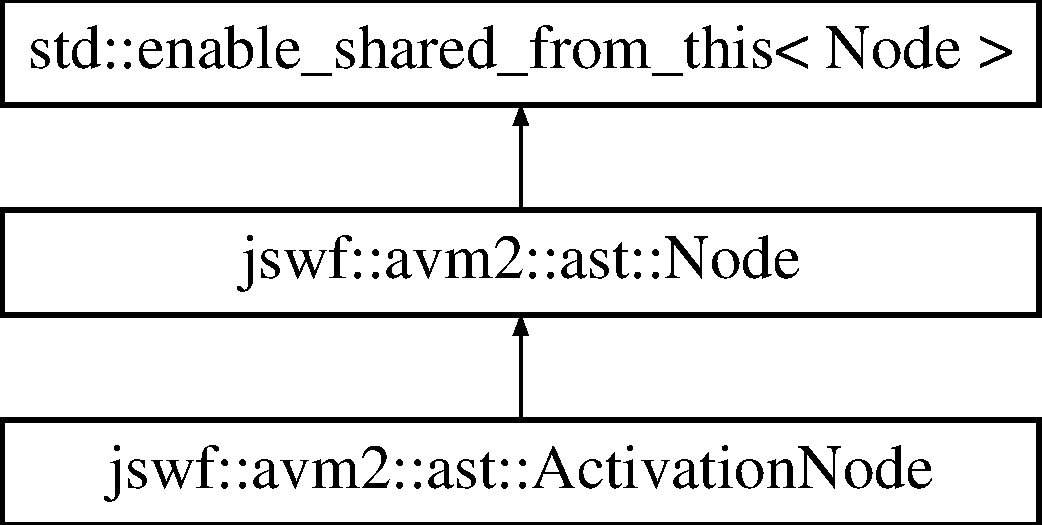
\includegraphics[height=3.000000cm]{classjswf_1_1avm2_1_1ast_1_1_activation_node}
\end{center}
\end{figure}
\subsection*{Public Member Functions}
\begin{DoxyCompactItemize}
\item 
\hypertarget{classjswf_1_1avm2_1_1ast_1_1_activation_node_addf599d16318841925cabd849c336251}{virtual std\+::string {\bfseries to\+String} ()}\label{classjswf_1_1avm2_1_1ast_1_1_activation_node_addf599d16318841925cabd849c336251}

\end{DoxyCompactItemize}
\subsection*{Additional Inherited Members}


\subsection{Detailed Description}
Describes an activation object. 

\begin{DoxyRefDesc}{Todo}
\item[\hyperlink{todo__todo000004}{Todo}]What is this? \end{DoxyRefDesc}


The documentation for this class was generated from the following file\+:\begin{DoxyCompactItemize}
\item 
jswf/avm2/ast/Node.\+h\end{DoxyCompactItemize}

\hypertarget{classjswf_1_1avm2_1_1ast_1_1_array_node}{\section{jswf\+:\+:avm2\+:\+:ast\+:\+:Array\+Node Class Reference}
\label{classjswf_1_1avm2_1_1ast_1_1_array_node}\index{jswf\+::avm2\+::ast\+::\+Array\+Node@{jswf\+::avm2\+::ast\+::\+Array\+Node}}
}


Describes an array literal.  




{\ttfamily \#include $<$Node.\+h$>$}

Inheritance diagram for jswf\+:\+:avm2\+:\+:ast\+:\+:Array\+Node\+:\begin{figure}[H]
\begin{center}
\leavevmode
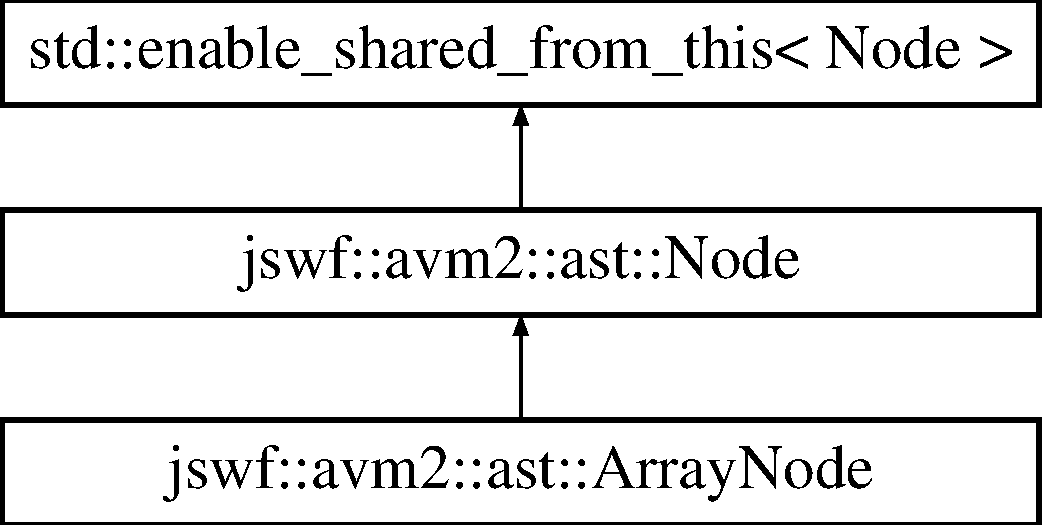
\includegraphics[height=3.000000cm]{classjswf_1_1avm2_1_1ast_1_1_array_node}
\end{center}
\end{figure}
\subsection*{Public Member Functions}
\begin{DoxyCompactItemize}
\item 
\hypertarget{classjswf_1_1avm2_1_1ast_1_1_array_node_a79b8767a5b409ada8c80836832b3c28e}{{\bfseries Array\+Node} (std\+::vector$<$ Node\+Ptr $>$ args)}\label{classjswf_1_1avm2_1_1ast_1_1_array_node_a79b8767a5b409ada8c80836832b3c28e}

\item 
\hypertarget{classjswf_1_1avm2_1_1ast_1_1_array_node_aa4e2db608958ce117252583675e5b950}{virtual std\+::string {\bfseries to\+String} ()}\label{classjswf_1_1avm2_1_1ast_1_1_array_node_aa4e2db608958ce117252583675e5b950}

\end{DoxyCompactItemize}
\subsection*{Public Attributes}
\begin{DoxyCompactItemize}
\item 
\hypertarget{classjswf_1_1avm2_1_1ast_1_1_array_node_a4125e463724e470c2b35db90abfbbe25}{std\+::vector$<$ Node\+Ptr $>$ {\bfseries arguments}}\label{classjswf_1_1avm2_1_1ast_1_1_array_node_a4125e463724e470c2b35db90abfbbe25}

\end{DoxyCompactItemize}


\subsection{Detailed Description}
Describes an array literal. 

The documentation for this class was generated from the following file\+:\begin{DoxyCompactItemize}
\item 
jswf/avm2/ast/Node.\+h\end{DoxyCompactItemize}

\hypertarget{classjswf_1_1avm2_1_1_array_object}{\section{jswf\+:\+:avm2\+:\+:Array\+Object Class Reference}
\label{classjswf_1_1avm2_1_1_array_object}\index{jswf\+::avm2\+::\+Array\+Object@{jswf\+::avm2\+::\+Array\+Object}}
}
Inheritance diagram for jswf\+:\+:avm2\+:\+:Array\+Object\+:\begin{figure}[H]
\begin{center}
\leavevmode
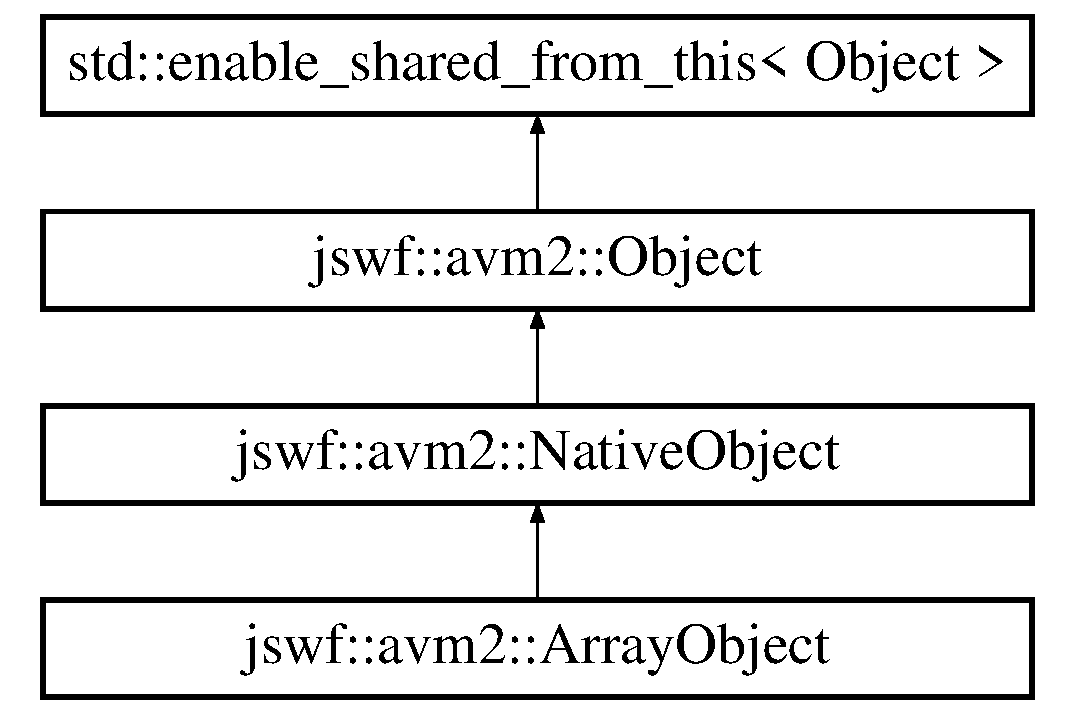
\includegraphics[height=4.000000cm]{classjswf_1_1avm2_1_1_array_object}
\end{center}
\end{figure}
\subsection*{Public Member Functions}
\begin{DoxyCompactItemize}
\item 
\hypertarget{classjswf_1_1avm2_1_1_array_object_a40dfb5f661e807f95060add2688d6134}{{\bfseries Array\+Object} (\hyperlink{classjswf_1_1avm2_1_1_v_m}{V\+M} $\ast$vm, const std\+::vector$<$ Object\+Ptr $>$ \&value)}\label{classjswf_1_1avm2_1_1_array_object_a40dfb5f661e807f95060add2688d6134}

\item 
\hypertarget{classjswf_1_1avm2_1_1_array_object_a45a025fba48de3584e031b53ec45baea}{std\+::vector$<$ Object\+Ptr $>$ {\bfseries coerce\+\_\+a} () const }\label{classjswf_1_1avm2_1_1_array_object_a45a025fba48de3584e031b53ec45baea}

\end{DoxyCompactItemize}
\subsection*{Public Attributes}
\begin{DoxyCompactItemize}
\item 
\hypertarget{classjswf_1_1avm2_1_1_array_object_a2153f43610d8e7da419d8f8b42e490ef}{std\+::vector$<$ Object\+Ptr $>$ {\bfseries value}}\label{classjswf_1_1avm2_1_1_array_object_a2153f43610d8e7da419d8f8b42e490ef}

\end{DoxyCompactItemize}
\subsection*{Additional Inherited Members}


The documentation for this class was generated from the following files\+:\begin{DoxyCompactItemize}
\item 
jswf/avm2/Object.\+h\item 
jswf/avm2/Object.\+cpp\end{DoxyCompactItemize}

\hypertarget{classjswf_1_1avm2_1_1ast_1_1_attr_node}{\section{jswf\+:\+:avm2\+:\+:ast\+:\+:Attr\+Node Class Reference}
\label{classjswf_1_1avm2_1_1ast_1_1_attr_node}\index{jswf\+::avm2\+::ast\+::\+Attr\+Node@{jswf\+::avm2\+::ast\+::\+Attr\+Node}}
}


Describes a property retrieved from an object.  




{\ttfamily \#include $<$Node.\+h$>$}

Inheritance diagram for jswf\+:\+:avm2\+:\+:ast\+:\+:Attr\+Node\+:\begin{figure}[H]
\begin{center}
\leavevmode
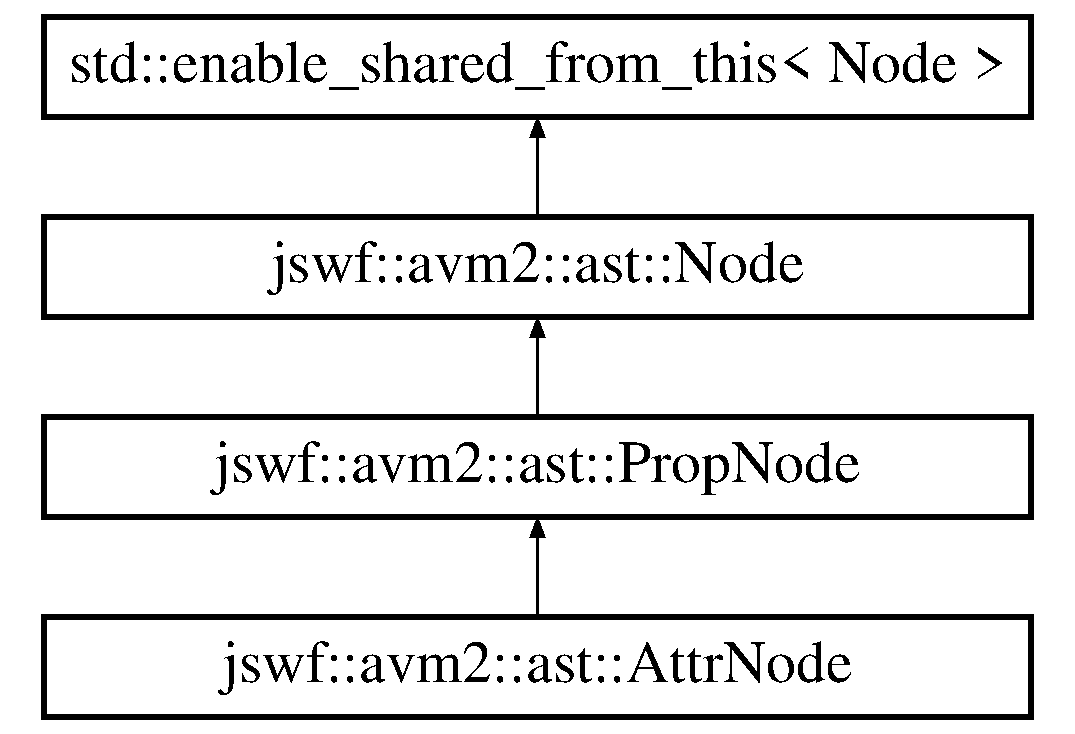
\includegraphics[height=4.000000cm]{classjswf_1_1avm2_1_1ast_1_1_attr_node}
\end{center}
\end{figure}
\subsection*{Public Member Functions}
\begin{DoxyCompactItemize}
\item 
\hypertarget{classjswf_1_1avm2_1_1ast_1_1_attr_node_ae80534f276b907a5152fda014a700046}{{\bfseries Attr\+Node} (Node\+Ptr obj, const \hyperlink{structjswf_1_1avm2_1_1_multiname}{Multiname} \&mn)}\label{classjswf_1_1avm2_1_1ast_1_1_attr_node_ae80534f276b907a5152fda014a700046}

\item 
\hypertarget{classjswf_1_1avm2_1_1ast_1_1_attr_node_a4ea079134d2ba0203e0bcc9504867cf3}{virtual std\+::string {\bfseries to\+String} ()}\label{classjswf_1_1avm2_1_1ast_1_1_attr_node_a4ea079134d2ba0203e0bcc9504867cf3}

\end{DoxyCompactItemize}
\subsection*{Public Attributes}
\begin{DoxyCompactItemize}
\item 
\hypertarget{classjswf_1_1avm2_1_1ast_1_1_attr_node_a1ba2f869002fc01715d80c5364026f9f}{Node\+Ptr {\bfseries obj}}\label{classjswf_1_1avm2_1_1ast_1_1_attr_node_a1ba2f869002fc01715d80c5364026f9f}

\end{DoxyCompactItemize}


\subsection{Detailed Description}
Describes a property retrieved from an object. 

\begin{DoxyRefDesc}{Todo}
\item[\hyperlink{todo__todo000002}{Todo}]Why not combine this with object? \end{DoxyRefDesc}


The documentation for this class was generated from the following file\+:\begin{DoxyCompactItemize}
\item 
jswf/avm2/ast/Node.\+h\end{DoxyCompactItemize}

\hypertarget{classjswf_1_1flash_1_1styles_1_1_bitmap_fill_style}{\section{jswf\+:\+:flash\+:\+:styles\+:\+:Bitmap\+Fill\+Style Class Reference}
\label{classjswf_1_1flash_1_1styles_1_1_bitmap_fill_style}\index{jswf\+::flash\+::styles\+::\+Bitmap\+Fill\+Style@{jswf\+::flash\+::styles\+::\+Bitmap\+Fill\+Style}}
}
Inheritance diagram for jswf\+:\+:flash\+:\+:styles\+:\+:Bitmap\+Fill\+Style\+:\begin{figure}[H]
\begin{center}
\leavevmode
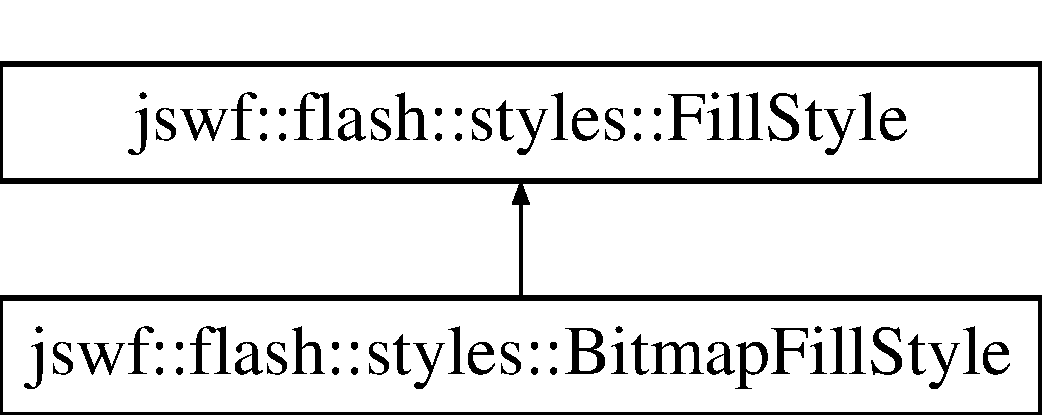
\includegraphics[height=2.000000cm]{classjswf_1_1flash_1_1styles_1_1_bitmap_fill_style}
\end{center}
\end{figure}
\subsection*{Public Attributes}
\begin{DoxyCompactItemize}
\item 
\hypertarget{classjswf_1_1flash_1_1styles_1_1_bitmap_fill_style_acdc7898f873830baa36cfe477779b0ce}{uint16\+\_\+t {\bfseries bitmap\+Id}}\label{classjswf_1_1flash_1_1styles_1_1_bitmap_fill_style_acdc7898f873830baa36cfe477779b0ce}

\item 
\hypertarget{classjswf_1_1flash_1_1styles_1_1_bitmap_fill_style_a8b27d3ace4d9a9c3cc925a4b158c75a3}{\hyperlink{structjswf_1_1flash_1_1_matrix}{Matrix} {\bfseries matrix}}\label{classjswf_1_1flash_1_1styles_1_1_bitmap_fill_style_a8b27d3ace4d9a9c3cc925a4b158c75a3}

\item 
\hypertarget{classjswf_1_1flash_1_1styles_1_1_bitmap_fill_style_a26f5c5903a21787e4ff280be30488fcb}{bool {\bfseries repeat}}\label{classjswf_1_1flash_1_1styles_1_1_bitmap_fill_style_a26f5c5903a21787e4ff280be30488fcb}

\item 
\hypertarget{classjswf_1_1flash_1_1styles_1_1_bitmap_fill_style_a7b8c7ea87b7784c57445677c3bfddf0b}{bool {\bfseries smooth}}\label{classjswf_1_1flash_1_1styles_1_1_bitmap_fill_style_a7b8c7ea87b7784c57445677c3bfddf0b}

\end{DoxyCompactItemize}


The documentation for this class was generated from the following file\+:\begin{DoxyCompactItemize}
\item 
jswf/flash/styles/Fill\+Style.\+h\end{DoxyCompactItemize}

\hypertarget{structjswf_1_1avm2_1_1_block}{\section{jswf\+:\+:avm2\+:\+:Block Struct Reference}
\label{structjswf_1_1avm2_1_1_block}\index{jswf\+::avm2\+::\+Block@{jswf\+::avm2\+::\+Block}}
}
\subsection*{Public Member Functions}
\begin{DoxyCompactItemize}
\item 
\hypertarget{structjswf_1_1avm2_1_1_block_a936e55b309066dbec37d0cd7be0ad4e4}{{\bfseries Block} (size\+\_\+t id, size\+\_\+t start)}\label{structjswf_1_1avm2_1_1_block_a936e55b309066dbec37d0cd7be0ad4e4}

\end{DoxyCompactItemize}
\subsection*{Public Attributes}
\begin{DoxyCompactItemize}
\item 
\hypertarget{structjswf_1_1avm2_1_1_block_a290876d59bc492ba250354b21688b8db}{size\+\_\+t {\bfseries id}}\label{structjswf_1_1avm2_1_1_block_a290876d59bc492ba250354b21688b8db}

\item 
\hypertarget{structjswf_1_1avm2_1_1_block_a75aec481cf4486cdac7bd3e38398c6e0}{bool {\bfseries analyzed} = false}\label{structjswf_1_1avm2_1_1_block_a75aec481cf4486cdac7bd3e38398c6e0}

\item 
\hypertarget{structjswf_1_1avm2_1_1_block_a9ef0c80f44de0a6d6070cbdd29dcb8f2}{size\+\_\+t {\bfseries start}}\label{structjswf_1_1avm2_1_1_block_a9ef0c80f44de0a6d6070cbdd29dcb8f2}

\item 
\hypertarget{structjswf_1_1avm2_1_1_block_ae9bb52bb058c2d5af26d3d93f3673123}{size\+\_\+t {\bfseries end}}\label{structjswf_1_1avm2_1_1_block_ae9bb52bb058c2d5af26d3d93f3673123}

\item 
\hypertarget{structjswf_1_1avm2_1_1_block_a6b54112adfc2757fc0b401de5e32d5eb}{std\+::vector$<$ \hyperlink{structjswf_1_1avm2_1_1_block}{Block} $\ast$ $>$ {\bfseries predecessors}}\label{structjswf_1_1avm2_1_1_block_a6b54112adfc2757fc0b401de5e32d5eb}

\item 
\hypertarget{structjswf_1_1avm2_1_1_block_ad00b93c78fadd59af5f4a4387e6a81a5}{std\+::vector$<$ \hyperlink{structjswf_1_1avm2_1_1_block}{Block} $\ast$ $>$ {\bfseries successors}}\label{structjswf_1_1avm2_1_1_block_ad00b93c78fadd59af5f4a4387e6a81a5}

\item 
\hypertarget{structjswf_1_1avm2_1_1_block_a64c986144de01fb844d2c382d01659d8}{int {\bfseries stack\+Balance} = 0}\label{structjswf_1_1avm2_1_1_block_a64c986144de01fb844d2c382d01659d8}

\item 
\hypertarget{structjswf_1_1avm2_1_1_block_a6374ab7364ec35c54e6851a94b1e4a7a}{int {\bfseries stack\+Min} = 0}\label{structjswf_1_1avm2_1_1_block_a6374ab7364ec35c54e6851a94b1e4a7a}

\item 
\hypertarget{structjswf_1_1avm2_1_1_block_a2bc6f951b252abfce8217d3ab30671d5}{int {\bfseries stack\+Max} = 0}\label{structjswf_1_1avm2_1_1_block_a2bc6f951b252abfce8217d3ab30671d5}

\end{DoxyCompactItemize}


The documentation for this struct was generated from the following file\+:\begin{DoxyCompactItemize}
\item 
jswf/avm2/\hyperlink{_verifier_8h}{Verifier.\+h}\end{DoxyCompactItemize}

\hypertarget{classjswf_1_1avm2_1_1_boolean_object}{\section{jswf\+:\+:avm2\+:\+:Boolean\+Object Class Reference}
\label{classjswf_1_1avm2_1_1_boolean_object}\index{jswf\+::avm2\+::\+Boolean\+Object@{jswf\+::avm2\+::\+Boolean\+Object}}
}


Represents a boolean (E\+C\+M\+A-\/262, section 8.\+3 {\itshape The Boolean Type}).  




{\ttfamily \#include $<$Object.\+h$>$}

Inheritance diagram for jswf\+:\+:avm2\+:\+:Boolean\+Object\+:\begin{figure}[H]
\begin{center}
\leavevmode
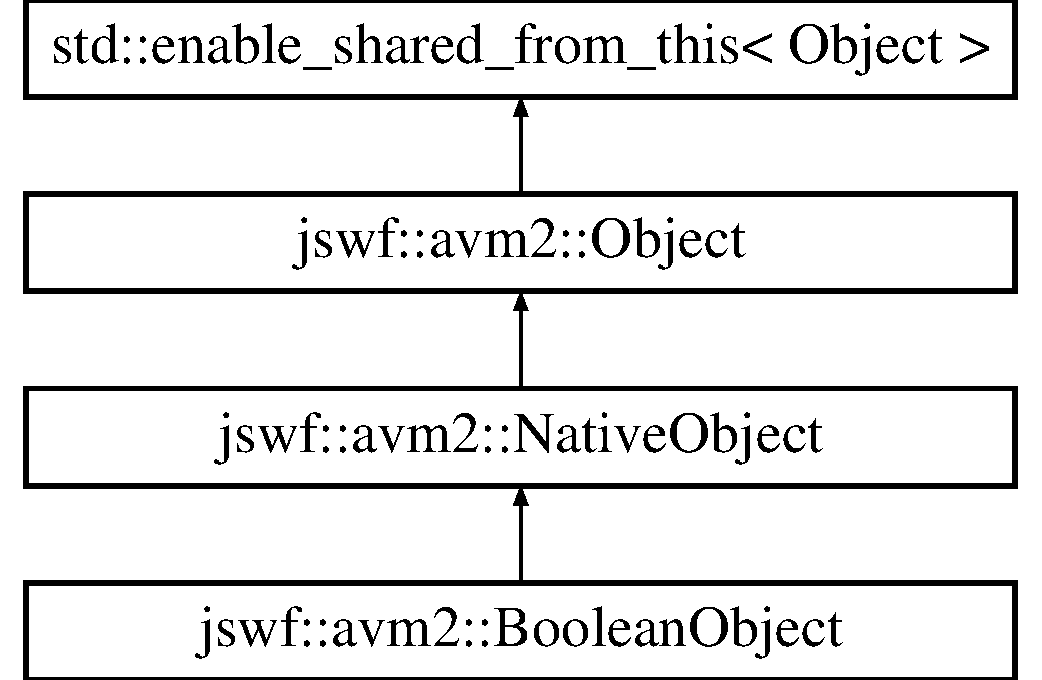
\includegraphics[height=4.000000cm]{classjswf_1_1avm2_1_1_boolean_object}
\end{center}
\end{figure}
\subsection*{Public Member Functions}
\begin{DoxyCompactItemize}
\item 
\hypertarget{classjswf_1_1avm2_1_1_boolean_object_aba0705eeb952a8474af409f0192dd725}{{\bfseries Boolean\+Object} (\hyperlink{classjswf_1_1avm2_1_1_v_m}{V\+M} $\ast$vm, const bool \&value)}\label{classjswf_1_1avm2_1_1_boolean_object_aba0705eeb952a8474af409f0192dd725}

\item 
\hypertarget{classjswf_1_1avm2_1_1_boolean_object_a8ebf06712c74f371f34e6fbe8fa7dfb3}{bool \hyperlink{classjswf_1_1avm2_1_1_boolean_object_a8ebf06712c74f371f34e6fbe8fa7dfb3}{coerce\+\_\+b} () const }\label{classjswf_1_1avm2_1_1_boolean_object_a8ebf06712c74f371f34e6fbe8fa7dfb3}

\begin{DoxyCompactList}\small\item\em Converts to {\ttfamily bool} (E\+C\+M\+A-\/262, section 9.\+2 {\itshape To\+Boolean}) \end{DoxyCompactList}\item 
std\+::string \hyperlink{classjswf_1_1avm2_1_1_boolean_object_a15d8e6b43434b3946e6fc377ba14a232}{coerce\+\_\+s} () const 
\begin{DoxyCompactList}\small\item\em Converts to {\ttfamily std\+::string} (E\+C\+M\+A-\/262, section 9.\+8 {\itshape To\+String}) \end{DoxyCompactList}\item 
\hypertarget{classjswf_1_1avm2_1_1_boolean_object_adcda0d16e0f3d549066510b58c95534f}{double \hyperlink{classjswf_1_1avm2_1_1_boolean_object_adcda0d16e0f3d549066510b58c95534f}{coerce\+\_\+d} () const }\label{classjswf_1_1avm2_1_1_boolean_object_adcda0d16e0f3d549066510b58c95534f}

\begin{DoxyCompactList}\small\item\em Converts to {\ttfamily double} (E\+C\+M\+A-\/262, section 9.\+3 {\itshape To\+Number}) \end{DoxyCompactList}\item 
\hypertarget{classjswf_1_1avm2_1_1_boolean_object_a7054f801b0c561873d983bf9c5c6b642}{bool {\bfseries same\+Type\+Equals} (const \hyperlink{classjswf_1_1avm2_1_1_object}{Object} \&rhs) const }\label{classjswf_1_1avm2_1_1_boolean_object_a7054f801b0c561873d983bf9c5c6b642}

\item 
\hypertarget{classjswf_1_1avm2_1_1_boolean_object_a6c86d27185f7d4c890515a7156e8af5b}{bool {\bfseries same\+Type\+Strict\+Equals} (const \hyperlink{classjswf_1_1avm2_1_1_object}{Object} \&rhs) const }\label{classjswf_1_1avm2_1_1_boolean_object_a6c86d27185f7d4c890515a7156e8af5b}

\end{DoxyCompactItemize}
\subsection*{Public Attributes}
\begin{DoxyCompactItemize}
\item 
\hypertarget{classjswf_1_1avm2_1_1_boolean_object_a88373d69dde0bf73948467de0a53f495}{bool {\bfseries value}}\label{classjswf_1_1avm2_1_1_boolean_object_a88373d69dde0bf73948467de0a53f495}

\end{DoxyCompactItemize}
\subsection*{Additional Inherited Members}


\subsection{Detailed Description}
Represents a boolean (E\+C\+M\+A-\/262, section 8.\+3 {\itshape The Boolean Type}). 

\subsection{Member Function Documentation}
\hypertarget{classjswf_1_1avm2_1_1_boolean_object_a15d8e6b43434b3946e6fc377ba14a232}{\index{jswf\+::avm2\+::\+Boolean\+Object@{jswf\+::avm2\+::\+Boolean\+Object}!coerce\+\_\+s@{coerce\+\_\+s}}
\index{coerce\+\_\+s@{coerce\+\_\+s}!jswf\+::avm2\+::\+Boolean\+Object@{jswf\+::avm2\+::\+Boolean\+Object}}
\subsubsection[{coerce\+\_\+s}]{\setlength{\rightskip}{0pt plus 5cm}std\+::string jswf\+::avm2\+::\+Boolean\+Object\+::coerce\+\_\+s (
\begin{DoxyParamCaption}
{}
\end{DoxyParamCaption}
) const\hspace{0.3cm}{\ttfamily [inline]}, {\ttfamily [virtual]}}}\label{classjswf_1_1avm2_1_1_boolean_object_a15d8e6b43434b3946e6fc377ba14a232}


Converts to {\ttfamily std\+::string} (E\+C\+M\+A-\/262, section 9.\+8 {\itshape To\+String}) 

\begin{DoxyRefDesc}{Todo}
\item[\hyperlink{todo__todo000007}{Todo}]Implement 9.\+8.\+1 \end{DoxyRefDesc}


Reimplemented from \hyperlink{classjswf_1_1avm2_1_1_object_a69b39776062acaccd2cd2b5a1f937c9d}{jswf\+::avm2\+::\+Object}.



The documentation for this class was generated from the following files\+:\begin{DoxyCompactItemize}
\item 
jswf/avm2/Object.\+h\item 
jswf/avm2/Object.\+cpp\end{DoxyCompactItemize}

\hypertarget{classjswf_1_1avm2_1_1_builtin_method_object}{\section{jswf\+:\+:avm2\+:\+:Builtin\+Method\+Object Class Reference}
\label{classjswf_1_1avm2_1_1_builtin_method_object}\index{jswf\+::avm2\+::\+Builtin\+Method\+Object@{jswf\+::avm2\+::\+Builtin\+Method\+Object}}
}


Represents a method that is provided by the runtime.  




{\ttfamily \#include $<$Object.\+h$>$}

Inheritance diagram for jswf\+:\+:avm2\+:\+:Builtin\+Method\+Object\+:\begin{figure}[H]
\begin{center}
\leavevmode
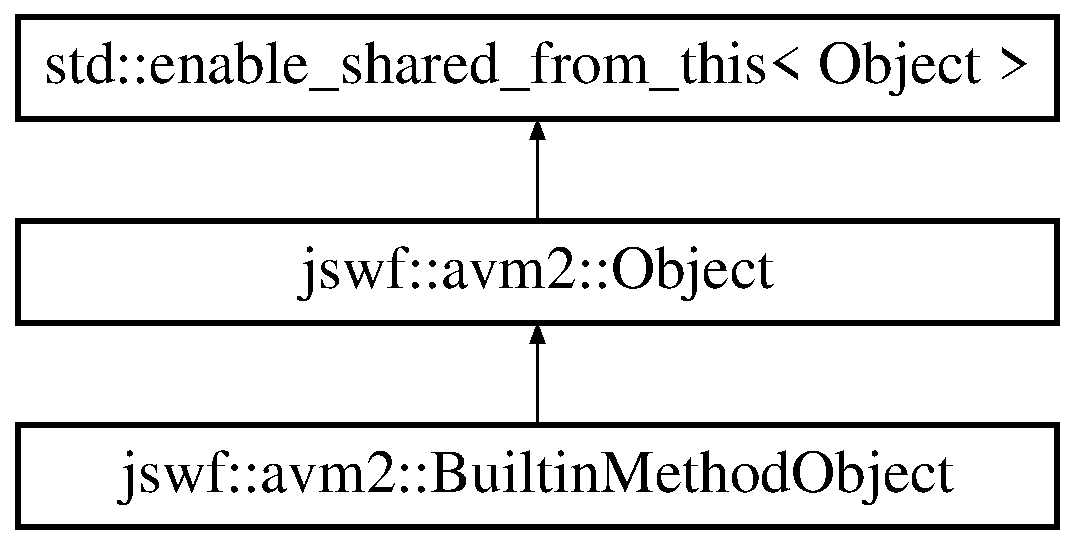
\includegraphics[height=3.000000cm]{classjswf_1_1avm2_1_1_builtin_method_object}
\end{center}
\end{figure}
\subsection*{Public Member Functions}
\begin{DoxyCompactItemize}
\item 
\hypertarget{classjswf_1_1avm2_1_1_builtin_method_object_a9dd3103382877771acf7e4832c9c428c}{{\bfseries Builtin\+Method\+Object} (\hyperlink{classjswf_1_1avm2_1_1_v_m}{V\+M} $\ast$vm, builtin\+\_\+method\+\_\+t $\ast$value)}\label{classjswf_1_1avm2_1_1_builtin_method_object_a9dd3103382877771acf7e4832c9c428c}

\item 
std\+::string \hyperlink{classjswf_1_1avm2_1_1_builtin_method_object_abd0021d91244a730a9275d1e690eed95}{coerce\+\_\+s} () const 
\begin{DoxyCompactList}\small\item\em Converts to {\ttfamily std\+::string} (E\+C\+M\+A-\/262, section 9.\+8 {\itshape To\+String}) \end{DoxyCompactList}\item 
\hypertarget{classjswf_1_1avm2_1_1_builtin_method_object_a76932e02bf47d2ca46bdf702d540d3f1}{Object\+Ptr {\bfseries ecma\+Call} (\hyperlink{classjswf_1_1avm2_1_1_v_m}{V\+M} \&vm, std\+::vector$<$ Object\+Ptr $>$ \&args) const }\label{classjswf_1_1avm2_1_1_builtin_method_object_a76932e02bf47d2ca46bdf702d540d3f1}

\end{DoxyCompactItemize}
\subsection*{Public Attributes}
\begin{DoxyCompactItemize}
\item 
\hypertarget{classjswf_1_1avm2_1_1_builtin_method_object_a836497cda54a772fc0e6cf1243b69960}{builtin\+\_\+method\+\_\+t $\ast$ {\bfseries value}}\label{classjswf_1_1avm2_1_1_builtin_method_object_a836497cda54a772fc0e6cf1243b69960}

\end{DoxyCompactItemize}
\subsection*{Additional Inherited Members}


\subsection{Detailed Description}
Represents a method that is provided by the runtime. 

\subsection{Member Function Documentation}
\hypertarget{classjswf_1_1avm2_1_1_builtin_method_object_abd0021d91244a730a9275d1e690eed95}{\index{jswf\+::avm2\+::\+Builtin\+Method\+Object@{jswf\+::avm2\+::\+Builtin\+Method\+Object}!coerce\+\_\+s@{coerce\+\_\+s}}
\index{coerce\+\_\+s@{coerce\+\_\+s}!jswf\+::avm2\+::\+Builtin\+Method\+Object@{jswf\+::avm2\+::\+Builtin\+Method\+Object}}
\subsubsection[{coerce\+\_\+s}]{\setlength{\rightskip}{0pt plus 5cm}std\+::string jswf\+::avm2\+::\+Builtin\+Method\+Object\+::coerce\+\_\+s (
\begin{DoxyParamCaption}
{}
\end{DoxyParamCaption}
) const\hspace{0.3cm}{\ttfamily [inline]}, {\ttfamily [virtual]}}}\label{classjswf_1_1avm2_1_1_builtin_method_object_abd0021d91244a730a9275d1e690eed95}


Converts to {\ttfamily std\+::string} (E\+C\+M\+A-\/262, section 9.\+8 {\itshape To\+String}) 

\begin{DoxyRefDesc}{Todo}
\item[\hyperlink{todo__todo000007}{Todo}]Implement 9.\+8.\+1 \end{DoxyRefDesc}


Reimplemented from \hyperlink{classjswf_1_1avm2_1_1_object_a69b39776062acaccd2cd2b5a1f937c9d}{jswf\+::avm2\+::\+Object}.



The documentation for this class was generated from the following files\+:\begin{DoxyCompactItemize}
\item 
jswf/avm2/Object.\+h\item 
jswf/avm2/Object.\+cpp\end{DoxyCompactItemize}

\hypertarget{classjswf_1_1flash_1_1_button}{\section{jswf\+:\+:flash\+:\+:Button Class Reference}
\label{classjswf_1_1flash_1_1_button}\index{jswf\+::flash\+::\+Button@{jswf\+::flash\+::\+Button}}
}


Represents a {\ttfamily B\+U\+T\+T\+O\+N} character.  




{\ttfamily \#include $<$Button.\+h$>$}

Inheritance diagram for jswf\+:\+:flash\+:\+:Button\+:\begin{figure}[H]
\begin{center}
\leavevmode
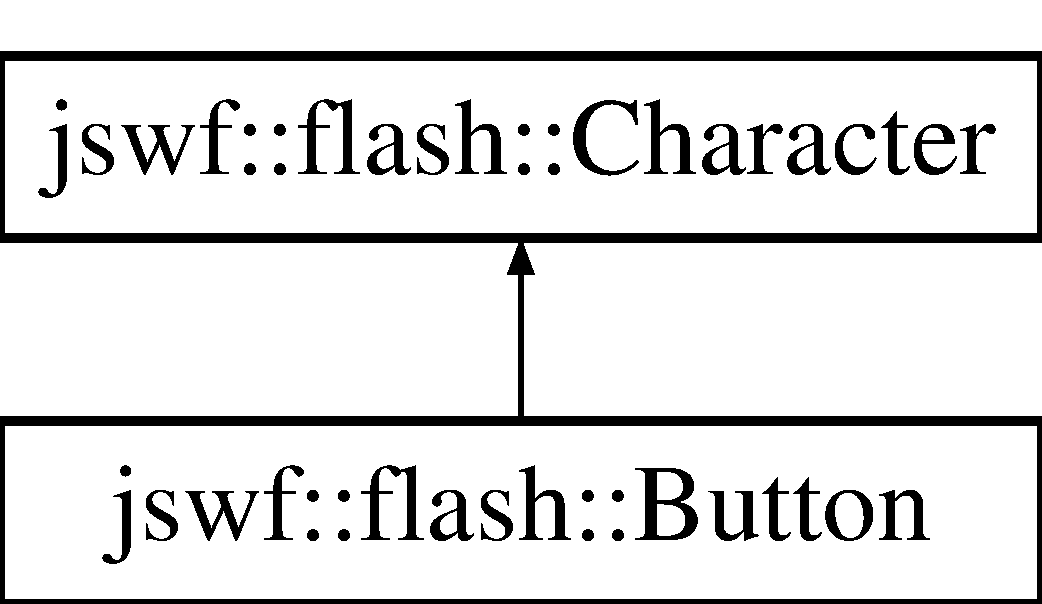
\includegraphics[height=2.000000cm]{classjswf_1_1flash_1_1_button}
\end{center}
\end{figure}
\subsection*{Public Types}
\begin{DoxyCompactItemize}
\item 
\hypertarget{classjswf_1_1flash_1_1_button_a9ac12df11e65243f4e97de7bd18acca9}{enum {\bfseries State\+Enum} \{ {\bfseries Up\+State} = 0, 
{\bfseries Over\+State} = 1, 
{\bfseries Down\+State} = 2, 
{\bfseries Hit\+Test\+State} = 3
 \}}\label{classjswf_1_1flash_1_1_button_a9ac12df11e65243f4e97de7bd18acca9}

\end{DoxyCompactItemize}
\subsection*{Public Attributes}
\begin{DoxyCompactItemize}
\item 
\hypertarget{classjswf_1_1flash_1_1_button_a0a347e9d44174d9febe1bfec6aa924de}{\hyperlink{classjswf_1_1flash_1_1_frame}{Frame} {\bfseries frames} \mbox{[}4\mbox{]}}\label{classjswf_1_1flash_1_1_button_a0a347e9d44174d9febe1bfec6aa924de}

\item 
\hypertarget{classjswf_1_1flash_1_1_button_a24fd84f8a74042d550f75c1021c1d2e4}{bool {\bfseries track\+As\+Menu} = false}\label{classjswf_1_1flash_1_1_button_a24fd84f8a74042d550f75c1021c1d2e4}

\end{DoxyCompactItemize}


\subsection{Detailed Description}
Represents a {\ttfamily B\+U\+T\+T\+O\+N} character. 

The documentation for this class was generated from the following file\+:\begin{DoxyCompactItemize}
\item 
jswf/flash/Button.\+h\end{DoxyCompactItemize}

\hypertarget{classjswf_1_1avm2_1_1ast_1_1_call_node}{\section{jswf\+:\+:avm2\+:\+:ast\+:\+:Call\+Node Class Reference}
\label{classjswf_1_1avm2_1_1ast_1_1_call_node}\index{jswf\+::avm2\+::ast\+::\+Call\+Node@{jswf\+::avm2\+::ast\+::\+Call\+Node}}
}


Describes a call to a function / method.  




{\ttfamily \#include $<$Node.\+h$>$}

Inheritance diagram for jswf\+:\+:avm2\+:\+:ast\+:\+:Call\+Node\+:\begin{figure}[H]
\begin{center}
\leavevmode
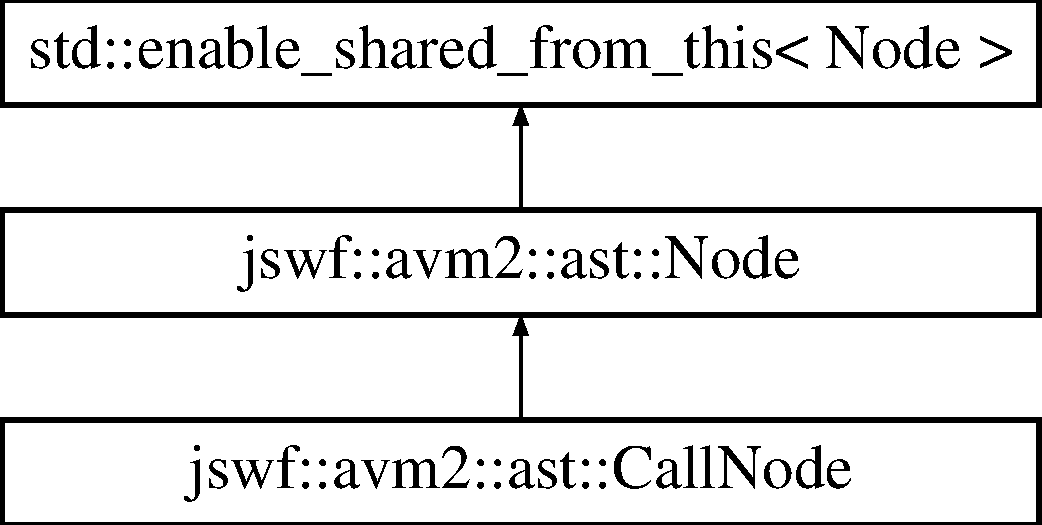
\includegraphics[height=3.000000cm]{classjswf_1_1avm2_1_1ast_1_1_call_node}
\end{center}
\end{figure}
\subsection*{Public Member Functions}
\begin{DoxyCompactItemize}
\item 
\hypertarget{classjswf_1_1avm2_1_1ast_1_1_call_node_a5f2357c66a001cd7adcdfe9199c2fc0f}{{\bfseries Call\+Node} (Node\+Ptr method, std\+::vector$<$ Node\+Ptr $>$ args)}\label{classjswf_1_1avm2_1_1ast_1_1_call_node_a5f2357c66a001cd7adcdfe9199c2fc0f}

\item 
\hypertarget{classjswf_1_1avm2_1_1ast_1_1_call_node_a30e5d5d240b04bec3141baf4b73e3ad0}{virtual std\+::string {\bfseries to\+String} ()}\label{classjswf_1_1avm2_1_1ast_1_1_call_node_a30e5d5d240b04bec3141baf4b73e3ad0}

\end{DoxyCompactItemize}
\subsection*{Public Attributes}
\begin{DoxyCompactItemize}
\item 
\hypertarget{classjswf_1_1avm2_1_1ast_1_1_call_node_aed18b408f34bd922c48cefee450733ae}{Node\+Ptr {\bfseries method}}\label{classjswf_1_1avm2_1_1ast_1_1_call_node_aed18b408f34bd922c48cefee450733ae}

\item 
\hypertarget{classjswf_1_1avm2_1_1ast_1_1_call_node_ab44f3a4d1823c468ebbf2fb5880d7c26}{std\+::vector$<$ Node\+Ptr $>$ {\bfseries arguments}}\label{classjswf_1_1avm2_1_1ast_1_1_call_node_ab44f3a4d1823c468ebbf2fb5880d7c26}

\end{DoxyCompactItemize}


\subsection{Detailed Description}
Describes a call to a function / method. 

The documentation for this class was generated from the following file\+:\begin{DoxyCompactItemize}
\item 
jswf/avm2/ast/Node.\+h\end{DoxyCompactItemize}

\hypertarget{classjswf_1_1flash_1_1_character}{\section{jswf\+:\+:flash\+:\+:Character Class Reference}
\label{classjswf_1_1flash_1_1_character}\index{jswf\+::flash\+::\+Character@{jswf\+::flash\+::\+Character}}
}


Represents a character for the document's {\ttfamily D\+I\+C\+T\+I\+O\+N\+A\+R\+Y}.  




{\ttfamily \#include $<$Character.\+h$>$}

Inheritance diagram for jswf\+:\+:flash\+:\+:Character\+:\begin{figure}[H]
\begin{center}
\leavevmode
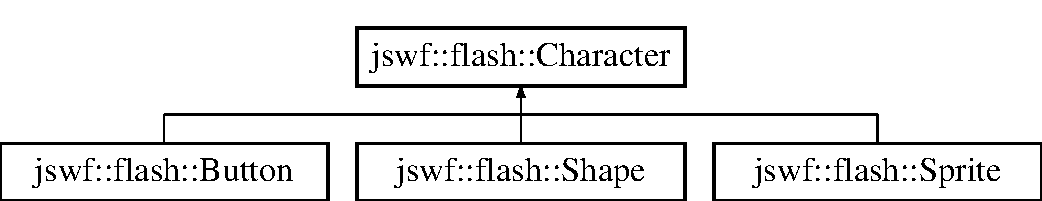
\includegraphics[height=2.000000cm]{classjswf_1_1flash_1_1_character}
\end{center}
\end{figure}
\subsection*{Public Attributes}
\begin{DoxyCompactItemize}
\item 
\hypertarget{classjswf_1_1flash_1_1_character_afa7b888be7a630ddd7a3efce690972f9}{\hyperlink{classjswf_1_1avm2_1_1_class}{avm2\+::\+Class} $\ast$ {\bfseries avm2\+Class} = N\+U\+L\+L}\label{classjswf_1_1flash_1_1_character_afa7b888be7a630ddd7a3efce690972f9}

\item 
\hypertarget{classjswf_1_1flash_1_1_character_a6583f97041d1b876721aed1e6e2b51a4}{uint16\+\_\+t {\bfseries id}}\label{classjswf_1_1flash_1_1_character_a6583f97041d1b876721aed1e6e2b51a4}

\end{DoxyCompactItemize}


\subsection{Detailed Description}
Represents a character for the document's {\ttfamily D\+I\+C\+T\+I\+O\+N\+A\+R\+Y}. 

The documentation for this class was generated from the following file\+:\begin{DoxyCompactItemize}
\item 
jswf/flash/Character.\+h\end{DoxyCompactItemize}

\hypertarget{classjswf_1_1avm2_1_1_class}{\section{jswf\+:\+:avm2\+:\+:Class Class Reference}
\label{classjswf_1_1avm2_1_1_class}\index{jswf\+::avm2\+::\+Class@{jswf\+::avm2\+::\+Class}}
}
\subsection*{Public Attributes}
\begin{DoxyCompactItemize}
\item 
\hypertarget{classjswf_1_1avm2_1_1_class_ae69515cce4632999d54a061aa1830a15}{\hyperlink{classjswf_1_1avm2_1_1_a_b_c_file}{A\+B\+C\+File} $\ast$ {\bfseries file}}\label{classjswf_1_1avm2_1_1_class_ae69515cce4632999d54a061aa1830a15}

\item 
\hypertarget{classjswf_1_1avm2_1_1_class_aa3351c4c1697cc2865094e45945cd26a}{\hyperlink{classjswf_1_1avm2_1_1_class}{Class} $\ast$ {\bfseries parent}}\label{classjswf_1_1avm2_1_1_class_aa3351c4c1697cc2865094e45945cd26a}

\item 
\hypertarget{classjswf_1_1avm2_1_1_class_ad083ce63da0ee72ab927bdb9584b4c51}{\hyperlink{classjswf_1_1avm2_1_1_v_m}{V\+M} $\ast$ {\bfseries vm}}\label{classjswf_1_1avm2_1_1_class_ad083ce63da0ee72ab927bdb9584b4c51}

\item 
\hypertarget{classjswf_1_1avm2_1_1_class_a2934c683c21c7178b0ee020b3f714f73}{\hyperlink{structjswf_1_1avm2_1_1_class_info}{Class\+Info} {\bfseries cinfo}}\label{classjswf_1_1avm2_1_1_class_a2934c683c21c7178b0ee020b3f714f73}

\item 
\hypertarget{classjswf_1_1avm2_1_1_class_ad4c29064adffcceb8a845babf3adfc22}{\hyperlink{structjswf_1_1avm2_1_1_instance_info}{Instance\+Info} {\bfseries iinfo}}\label{classjswf_1_1avm2_1_1_class_ad4c29064adffcceb8a845babf3adfc22}

\item 
\hypertarget{classjswf_1_1avm2_1_1_class_af87bce2a4540cc8ab8cdc8e04816ef02}{Trait\+Map {\bfseries trait\+Map}}\label{classjswf_1_1avm2_1_1_class_af87bce2a4540cc8ab8cdc8e04816ef02}

\item 
\hypertarget{classjswf_1_1avm2_1_1_class_a3fb41570194ccecc2b325fff07f2a4ff}{Slot\+Map {\bfseries slot\+Map}}\label{classjswf_1_1avm2_1_1_class_a3fb41570194ccecc2b325fff07f2a4ff}

\end{DoxyCompactItemize}


The documentation for this class was generated from the following file\+:\begin{DoxyCompactItemize}
\item 
jswf/avm2/A\+B\+C\+File.\+h\end{DoxyCompactItemize}

\hypertarget{structjswf_1_1avm2_1_1_class_info}{\section{jswf\+:\+:avm2\+:\+:Class\+Info Struct Reference}
\label{structjswf_1_1avm2_1_1_class_info}\index{jswf\+::avm2\+::\+Class\+Info@{jswf\+::avm2\+::\+Class\+Info}}
}
\subsection*{Public Attributes}
\begin{DoxyCompactItemize}
\item 
\hypertarget{structjswf_1_1avm2_1_1_class_info_ae91886322b2eedec321ecd9afbe733da}{\hyperlink{structjswf_1_1avm2_1_1_method_info}{Method\+Info} $\ast$ {\bfseries initializer}}\label{structjswf_1_1avm2_1_1_class_info_ae91886322b2eedec321ecd9afbe733da}

\item 
\hypertarget{structjswf_1_1avm2_1_1_class_info_aee121f21193215013f853e8c409d81f9}{std\+::vector$<$ std\+::shared\+\_\+ptr\\*
$<$ \hyperlink{structjswf_1_1avm2_1_1_trait_info}{Trait\+Info} $>$ $>$ {\bfseries traits}}\label{structjswf_1_1avm2_1_1_class_info_aee121f21193215013f853e8c409d81f9}

\end{DoxyCompactItemize}


The documentation for this struct was generated from the following file\+:\begin{DoxyCompactItemize}
\item 
jswf/avm2/A\+B\+C\+File.\+h\end{DoxyCompactItemize}

\hypertarget{classjswf_1_1avm2_1_1_class_object}{\section{jswf\+:\+:avm2\+:\+:Class\+Object Class Reference}
\label{classjswf_1_1avm2_1_1_class_object}\index{jswf\+::avm2\+::\+Class\+Object@{jswf\+::avm2\+::\+Class\+Object}}
}


Represents a class.  




{\ttfamily \#include $<$Object.\+h$>$}

Inheritance diagram for jswf\+:\+:avm2\+:\+:Class\+Object\+:\begin{figure}[H]
\begin{center}
\leavevmode
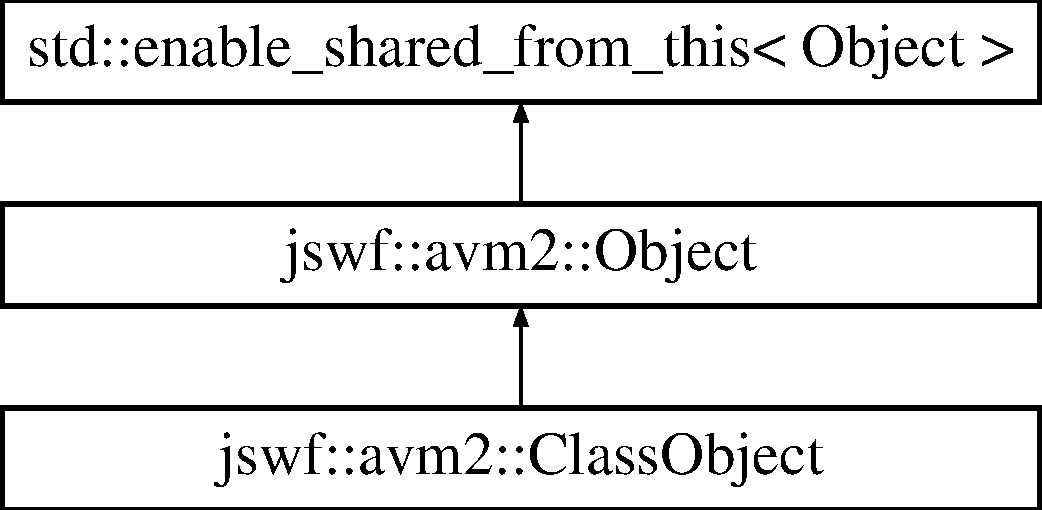
\includegraphics[height=3.000000cm]{classjswf_1_1avm2_1_1_class_object}
\end{center}
\end{figure}
\subsection*{Public Member Functions}
\begin{DoxyCompactItemize}
\item 
\hypertarget{classjswf_1_1avm2_1_1_class_object_a7c1bcfada2136ea23f6d34b4d11ce211}{{\bfseries Class\+Object} (\hyperlink{classjswf_1_1avm2_1_1_v_m}{V\+M} $\ast$vm, \hyperlink{classjswf_1_1avm2_1_1_class}{Class} $\ast$value)}\label{classjswf_1_1avm2_1_1_class_object_a7c1bcfada2136ea23f6d34b4d11ce211}

\item 
std\+::string \hyperlink{classjswf_1_1avm2_1_1_class_object_ad19a4ad7c166a694e0f0f349727fc9c2}{coerce\+\_\+s} () const 
\begin{DoxyCompactList}\small\item\em Converts to {\ttfamily std\+::string} (E\+C\+M\+A-\/262, section 9.\+8 {\itshape To\+String}) \end{DoxyCompactList}\end{DoxyCompactItemize}
\subsection*{Public Attributes}
\begin{DoxyCompactItemize}
\item 
\hypertarget{classjswf_1_1avm2_1_1_class_object_a8910e99a301c2caddd9334694d42acc5}{\hyperlink{classjswf_1_1avm2_1_1_class}{Class} $\ast$ {\bfseries value}}\label{classjswf_1_1avm2_1_1_class_object_a8910e99a301c2caddd9334694d42acc5}

\end{DoxyCompactItemize}
\subsection*{Additional Inherited Members}


\subsection{Detailed Description}
Represents a class. 

\subsection{Member Function Documentation}
\hypertarget{classjswf_1_1avm2_1_1_class_object_ad19a4ad7c166a694e0f0f349727fc9c2}{\index{jswf\+::avm2\+::\+Class\+Object@{jswf\+::avm2\+::\+Class\+Object}!coerce\+\_\+s@{coerce\+\_\+s}}
\index{coerce\+\_\+s@{coerce\+\_\+s}!jswf\+::avm2\+::\+Class\+Object@{jswf\+::avm2\+::\+Class\+Object}}
\subsubsection[{coerce\+\_\+s}]{\setlength{\rightskip}{0pt plus 5cm}std\+::string jswf\+::avm2\+::\+Class\+Object\+::coerce\+\_\+s (
\begin{DoxyParamCaption}
{}
\end{DoxyParamCaption}
) const\hspace{0.3cm}{\ttfamily [inline]}, {\ttfamily [virtual]}}}\label{classjswf_1_1avm2_1_1_class_object_ad19a4ad7c166a694e0f0f349727fc9c2}


Converts to {\ttfamily std\+::string} (E\+C\+M\+A-\/262, section 9.\+8 {\itshape To\+String}) 

\begin{DoxyRefDesc}{Todo}
\item[\hyperlink{todo__todo000007}{Todo}]Implement 9.\+8.\+1 \end{DoxyRefDesc}


Reimplemented from \hyperlink{classjswf_1_1avm2_1_1_object_a69b39776062acaccd2cd2b5a1f937c9d}{jswf\+::avm2\+::\+Object}.



The documentation for this class was generated from the following files\+:\begin{DoxyCompactItemize}
\item 
jswf/avm2/Object.\+h\item 
jswf/avm2/Object.\+cpp\end{DoxyCompactItemize}

\hypertarget{structjswf_1_1avm2_1_1_class_trait_info}{\section{jswf\+:\+:avm2\+:\+:Class\+Trait\+Info Struct Reference}
\label{structjswf_1_1avm2_1_1_class_trait_info}\index{jswf\+::avm2\+::\+Class\+Trait\+Info@{jswf\+::avm2\+::\+Class\+Trait\+Info}}
}
Inheritance diagram for jswf\+:\+:avm2\+:\+:Class\+Trait\+Info\+:\begin{figure}[H]
\begin{center}
\leavevmode
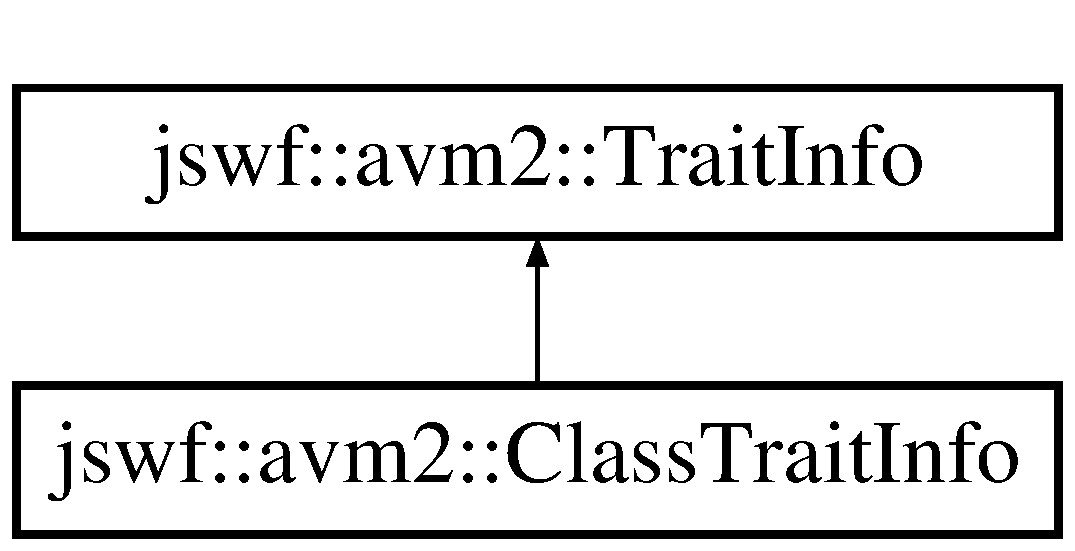
\includegraphics[height=2.000000cm]{structjswf_1_1avm2_1_1_class_trait_info}
\end{center}
\end{figure}
\subsection*{Public Attributes}
\begin{DoxyCompactItemize}
\item 
\hypertarget{structjswf_1_1avm2_1_1_class_trait_info_a40135fb7f7716180de046bb8d406fbf0}{\hyperlink{namespacejswf_aa10d9ddca2a6a5debdc261dfae3d1117}{u30\+\_\+t} {\bfseries slot\+Id}}\label{structjswf_1_1avm2_1_1_class_trait_info_a40135fb7f7716180de046bb8d406fbf0}

\item 
\hypertarget{structjswf_1_1avm2_1_1_class_trait_info_a0f3335d812d8829d2924b1e639aa719b}{\hyperlink{structjswf_1_1avm2_1_1_class_info}{Class\+Info} $\ast$ {\bfseries class\+Info}}\label{structjswf_1_1avm2_1_1_class_trait_info_a0f3335d812d8829d2924b1e639aa719b}

\end{DoxyCompactItemize}
\subsection*{Additional Inherited Members}


The documentation for this struct was generated from the following file\+:\begin{DoxyCompactItemize}
\item 
jswf/avm2/Trait\+Info.\+h\end{DoxyCompactItemize}

\hypertarget{structjswf_1_1flash_1_1_color_transform}{\section{jswf\+:\+:flash\+:\+:Color\+Transform Struct Reference}
\label{structjswf_1_1flash_1_1_color_transform}\index{jswf\+::flash\+::\+Color\+Transform@{jswf\+::flash\+::\+Color\+Transform}}
}


Represents {\ttfamily C\+X\+F\+O\+R\+M} and {\ttfamily C\+X\+F\+O\+R\+M\+W\+I\+T\+H\+A\+L\+P\+H\+A} records.  




{\ttfamily \#include $<$Structs.\+h$>$}

\subsection*{Public Attributes}
\begin{DoxyCompactItemize}
\item 
\hypertarget{structjswf_1_1flash_1_1_color_transform_ad0ecdb45c70244fd39e5619c5c72334a}{\hyperlink{namespacejswf_aa56b2b764590a9e19a5e66693364aceb}{sb\+\_\+t} {\bfseries r\+M} = 256}\label{structjswf_1_1flash_1_1_color_transform_ad0ecdb45c70244fd39e5619c5c72334a}

\item 
\hypertarget{structjswf_1_1flash_1_1_color_transform_a16f99356e12912f517a05ad94aebe9d9}{\hyperlink{namespacejswf_aa56b2b764590a9e19a5e66693364aceb}{sb\+\_\+t} {\bfseries r\+A} = 0}\label{structjswf_1_1flash_1_1_color_transform_a16f99356e12912f517a05ad94aebe9d9}

\item 
\hypertarget{structjswf_1_1flash_1_1_color_transform_aa4996da50294d5d429d1344c9e110c48}{\hyperlink{namespacejswf_aa56b2b764590a9e19a5e66693364aceb}{sb\+\_\+t} {\bfseries g\+M} = 256}\label{structjswf_1_1flash_1_1_color_transform_aa4996da50294d5d429d1344c9e110c48}

\item 
\hypertarget{structjswf_1_1flash_1_1_color_transform_a4d81df4e3fb8c403451eb01d048823c3}{\hyperlink{namespacejswf_aa56b2b764590a9e19a5e66693364aceb}{sb\+\_\+t} {\bfseries g\+A} = 0}\label{structjswf_1_1flash_1_1_color_transform_a4d81df4e3fb8c403451eb01d048823c3}

\item 
\hypertarget{structjswf_1_1flash_1_1_color_transform_ab3638b378433233e20e2ea9ab4ae7fbe}{\hyperlink{namespacejswf_aa56b2b764590a9e19a5e66693364aceb}{sb\+\_\+t} {\bfseries b\+M} = 256}\label{structjswf_1_1flash_1_1_color_transform_ab3638b378433233e20e2ea9ab4ae7fbe}

\item 
\hypertarget{structjswf_1_1flash_1_1_color_transform_aeb73b91261e6bd9d4b7631d95b8b8057}{\hyperlink{namespacejswf_aa56b2b764590a9e19a5e66693364aceb}{sb\+\_\+t} {\bfseries b\+A} = 0}\label{structjswf_1_1flash_1_1_color_transform_aeb73b91261e6bd9d4b7631d95b8b8057}

\item 
\hypertarget{structjswf_1_1flash_1_1_color_transform_a1cee972b5afae94dc1ef3c9c3cadaa01}{\hyperlink{namespacejswf_aa56b2b764590a9e19a5e66693364aceb}{sb\+\_\+t} {\bfseries a\+M} = 256}\label{structjswf_1_1flash_1_1_color_transform_a1cee972b5afae94dc1ef3c9c3cadaa01}

\item 
\hypertarget{structjswf_1_1flash_1_1_color_transform_a812d5db124ac1ec24b796be1798b03b7}{\hyperlink{namespacejswf_aa56b2b764590a9e19a5e66693364aceb}{sb\+\_\+t} {\bfseries a\+A} = 0}\label{structjswf_1_1flash_1_1_color_transform_a812d5db124ac1ec24b796be1798b03b7}

\end{DoxyCompactItemize}


\subsection{Detailed Description}
Represents {\ttfamily C\+X\+F\+O\+R\+M} and {\ttfamily C\+X\+F\+O\+R\+M\+W\+I\+T\+H\+A\+L\+P\+H\+A} records. 

For each channel $v$ from ${r,g,b,a}$, the transformed value $v'$ can be computed as follows\+:~\newline
 $v' = max(0, min((v \cdot vM \cdot \frac{1}{256}) + vA, 255))$ 

The documentation for this struct was generated from the following file\+:\begin{DoxyCompactItemize}
\item 
jswf/flash/\hyperlink{_structs_8h}{Structs.\+h}\end{DoxyCompactItemize}

\hypertarget{classjswf_1_1avm2_1_1ast_1_1_comment_node}{\section{jswf\+:\+:avm2\+:\+:ast\+:\+:Comment\+Node Class Reference}
\label{classjswf_1_1avm2_1_1ast_1_1_comment_node}\index{jswf\+::avm2\+::ast\+::\+Comment\+Node@{jswf\+::avm2\+::ast\+::\+Comment\+Node}}
}


Describes a comment statement.  




{\ttfamily \#include $<$Node.\+h$>$}

Inheritance diagram for jswf\+:\+:avm2\+:\+:ast\+:\+:Comment\+Node\+:\begin{figure}[H]
\begin{center}
\leavevmode
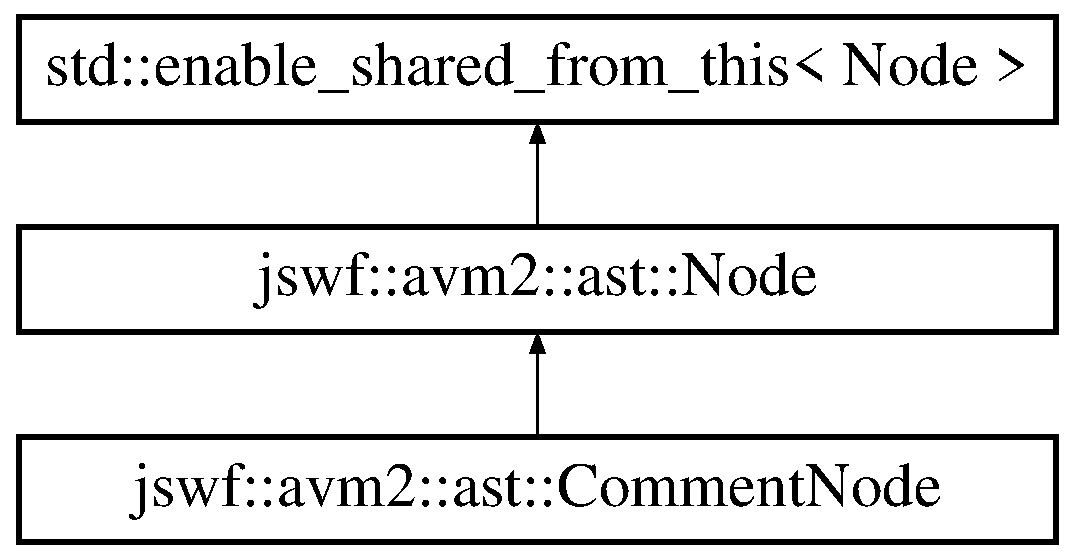
\includegraphics[height=3.000000cm]{classjswf_1_1avm2_1_1ast_1_1_comment_node}
\end{center}
\end{figure}
\subsection*{Public Member Functions}
\begin{DoxyCompactItemize}
\item 
\hypertarget{classjswf_1_1avm2_1_1ast_1_1_comment_node_adca471d5e1747ea23ac7a8ab838b7fab}{{\bfseries Comment\+Node} (std\+::string comment)}\label{classjswf_1_1avm2_1_1ast_1_1_comment_node_adca471d5e1747ea23ac7a8ab838b7fab}

\item 
\hypertarget{classjswf_1_1avm2_1_1ast_1_1_comment_node_a05c1d501f06fb65038d604d62caf7abb}{virtual std\+::string {\bfseries to\+String} ()}\label{classjswf_1_1avm2_1_1ast_1_1_comment_node_a05c1d501f06fb65038d604d62caf7abb}

\end{DoxyCompactItemize}
\subsection*{Public Attributes}
\begin{DoxyCompactItemize}
\item 
\hypertarget{classjswf_1_1avm2_1_1ast_1_1_comment_node_a90f211335c9b387e51ca632d6ed4ac42}{std\+::string {\bfseries comment}}\label{classjswf_1_1avm2_1_1ast_1_1_comment_node_a90f211335c9b387e51ca632d6ed4ac42}

\end{DoxyCompactItemize}


\subsection{Detailed Description}
Describes a comment statement. 

The documentation for this class was generated from the following file\+:\begin{DoxyCompactItemize}
\item 
jswf/avm2/ast/Node.\+h\end{DoxyCompactItemize}

\hypertarget{classjswf_1_1avm2_1_1ast_1_1_compound_node}{\section{jswf\+:\+:avm2\+:\+:ast\+:\+:Compound\+Node Class Reference}
\label{classjswf_1_1avm2_1_1ast_1_1_compound_node}\index{jswf\+::avm2\+::ast\+::\+Compound\+Node@{jswf\+::avm2\+::ast\+::\+Compound\+Node}}
}


Describes a node that contains statements.  




{\ttfamily \#include $<$Node.\+h$>$}

Inheritance diagram for jswf\+:\+:avm2\+:\+:ast\+:\+:Compound\+Node\+:\begin{figure}[H]
\begin{center}
\leavevmode
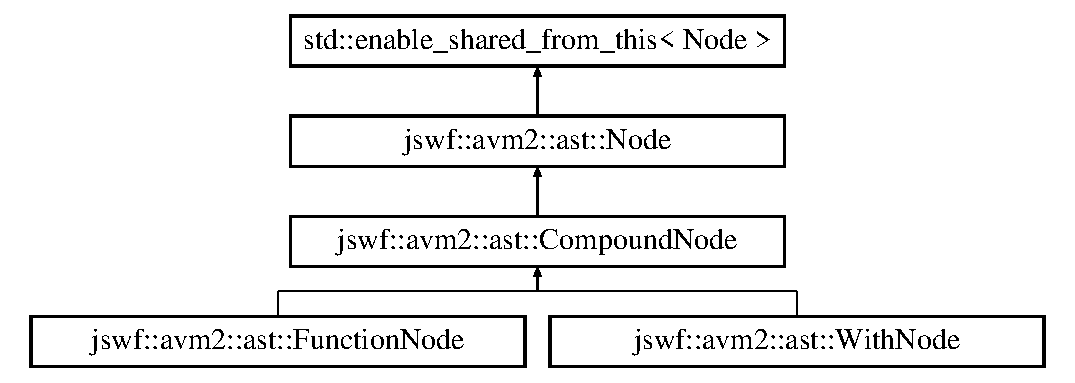
\includegraphics[height=4.000000cm]{classjswf_1_1avm2_1_1ast_1_1_compound_node}
\end{center}
\end{figure}
\subsection*{Public Member Functions}
\begin{DoxyCompactItemize}
\item 
\hypertarget{classjswf_1_1avm2_1_1ast_1_1_compound_node_a56af26ef9ff88b908db9f29e3b43bfea}{{\bfseries Compound\+Node} (int precedence)}\label{classjswf_1_1avm2_1_1ast_1_1_compound_node_a56af26ef9ff88b908db9f29e3b43bfea}

\item 
\hypertarget{classjswf_1_1avm2_1_1ast_1_1_compound_node_a0770f297a6c0058d9923076afae0ac27}{virtual std\+::string {\bfseries to\+String} ()}\label{classjswf_1_1avm2_1_1ast_1_1_compound_node_a0770f297a6c0058d9923076afae0ac27}

\item 
\hypertarget{classjswf_1_1avm2_1_1ast_1_1_compound_node_a76c1416f875841088773d18f2ecbffa9}{virtual std\+::string {\bfseries to\+Intended\+String} (int intend)}\label{classjswf_1_1avm2_1_1ast_1_1_compound_node_a76c1416f875841088773d18f2ecbffa9}

\end{DoxyCompactItemize}
\subsection*{Public Attributes}
\begin{DoxyCompactItemize}
\item 
\hypertarget{classjswf_1_1avm2_1_1ast_1_1_compound_node_a9ebf4cd8a31976e96fa1ce86402b1c4c}{\hyperlink{classjswf_1_1avm2_1_1ast_1_1_compound_node}{Compound\+Node} $\ast$ {\bfseries parent}}\label{classjswf_1_1avm2_1_1ast_1_1_compound_node_a9ebf4cd8a31976e96fa1ce86402b1c4c}

\item 
\hypertarget{classjswf_1_1avm2_1_1ast_1_1_compound_node_a6bd75515f8858dec99745eab8b5903b1}{std\+::vector$<$ Node\+Ptr $>$ {\bfseries body}}\label{classjswf_1_1avm2_1_1ast_1_1_compound_node_a6bd75515f8858dec99745eab8b5903b1}

\end{DoxyCompactItemize}


\subsection{Detailed Description}
Describes a node that contains statements. 

\begin{DoxyRefDesc}{Todo}
\item[\hyperlink{todo__todo000005}{Todo}]Make a statement node? \end{DoxyRefDesc}


The documentation for this class was generated from the following file\+:\begin{DoxyCompactItemize}
\item 
jswf/avm2/ast/Node.\+h\end{DoxyCompactItemize}

\hypertarget{structjswf_1_1flash_1_1_compression}{\section{jswf\+:\+:flash\+:\+:Compression Struct Reference}
\label{structjswf_1_1flash_1_1_compression}\index{jswf\+::flash\+::\+Compression@{jswf\+::flash\+::\+Compression}}
}


Provides \hyperlink{structjswf_1_1flash_1_1_compression_a393e4fe7bb01f081e0c1d1d009c22c2a}{Compression\+::\+Enum}.  




{\ttfamily \#include $<$Header.\+h$>$}

\subsection*{Public Types}
\begin{DoxyCompactItemize}
\item 
\hypertarget{structjswf_1_1flash_1_1_compression_a393e4fe7bb01f081e0c1d1d009c22c2a}{enum \hyperlink{structjswf_1_1flash_1_1_compression_a393e4fe7bb01f081e0c1d1d009c22c2a}{Enum} \{ {\bfseries Uncompressed}, 
{\bfseries Z\+Lib}
 \}}\label{structjswf_1_1flash_1_1_compression_a393e4fe7bb01f081e0c1d1d009c22c2a}

\begin{DoxyCompactList}\small\item\em Describes the kinds of compressions used by S\+W\+F documents. \end{DoxyCompactList}\end{DoxyCompactItemize}


\subsection{Detailed Description}
Provides \hyperlink{structjswf_1_1flash_1_1_compression_a393e4fe7bb01f081e0c1d1d009c22c2a}{Compression\+::\+Enum}. 

The documentation for this struct was generated from the following file\+:\begin{DoxyCompactItemize}
\item 
jswf/flash/Header.\+h\end{DoxyCompactItemize}

\hypertarget{structjswf_1_1avm2_1_1_constant_kind}{\section{jswf\+:\+:avm2\+:\+:Constant\+Kind Struct Reference}
\label{structjswf_1_1avm2_1_1_constant_kind}\index{jswf\+::avm2\+::\+Constant\+Kind@{jswf\+::avm2\+::\+Constant\+Kind}}
}
\subsection*{Public Types}
\begin{DoxyCompactItemize}
\item 
\hypertarget{structjswf_1_1avm2_1_1_constant_kind_a08c93a1e1d9466df91b4b9b70e0cc8b7}{enum {\bfseries Enum} \+: u8\+\_\+t \{ \\*
{\bfseries Int\+Kind} = 0x03, 
{\bfseries U\+Int\+Kind} = 0x04, 
{\bfseries Double\+Kind} = 0x06, 
{\bfseries U\+T\+F8\+Kind} = 0x01, 
\\*
{\bfseries False\+Kind} = 0x0a, 
{\bfseries True\+Kind} = 0x0b, 
{\bfseries Null\+Kind} = 0x0c, 
{\bfseries Undefined\+Kind} = 0x00, 
\\*
{\bfseries Normal\+Namespace\+Kind} = 0x08, 
{\bfseries Package\+Namespace\+Kind} = 0x16, 
{\bfseries Package\+Internal\+Ns\+Kind} = 0x17, 
{\bfseries Protected\+Namespace\+Kind} = 0x18, 
\\*
{\bfseries Explicit\+Namespace\+Kind} = 0x19, 
{\bfseries Static\+Protected\+Ns\+Kind} = 0x1a, 
{\bfseries Private\+Namespace\+Kind} = 0x05, 
{\bfseries N\+A\+N\+Kind} = 0x80, 
\\*
{\bfseries Byte\+Kind} = 0x81, 
{\bfseries Short\+Kind} = 0x82
 \}}\label{structjswf_1_1avm2_1_1_constant_kind_a08c93a1e1d9466df91b4b9b70e0cc8b7}

\end{DoxyCompactItemize}
\subsection*{Static Public Member Functions}
\begin{DoxyCompactItemize}
\item 
\hypertarget{structjswf_1_1avm2_1_1_constant_kind_a6c6a040fc9d7e1fd5cc0c296641fc5ce}{static bool {\bfseries needs\+Pool} (Constant\+Kind\+::\+Enum kind)}\label{structjswf_1_1avm2_1_1_constant_kind_a6c6a040fc9d7e1fd5cc0c296641fc5ce}

\end{DoxyCompactItemize}


The documentation for this struct was generated from the following file\+:\begin{DoxyCompactItemize}
\item 
jswf/avm2/Constant\+Kind.\+h\end{DoxyCompactItemize}

\hypertarget{classjswf_1_1avm2_1_1ast_1_1_constant_node}{\section{jswf\+:\+:avm2\+:\+:ast\+:\+:Constant\+Node Class Reference}
\label{classjswf_1_1avm2_1_1ast_1_1_constant_node}\index{jswf\+::avm2\+::ast\+::\+Constant\+Node@{jswf\+::avm2\+::ast\+::\+Constant\+Node}}
}
Inheritance diagram for jswf\+:\+:avm2\+:\+:ast\+:\+:Constant\+Node\+:\begin{figure}[H]
\begin{center}
\leavevmode
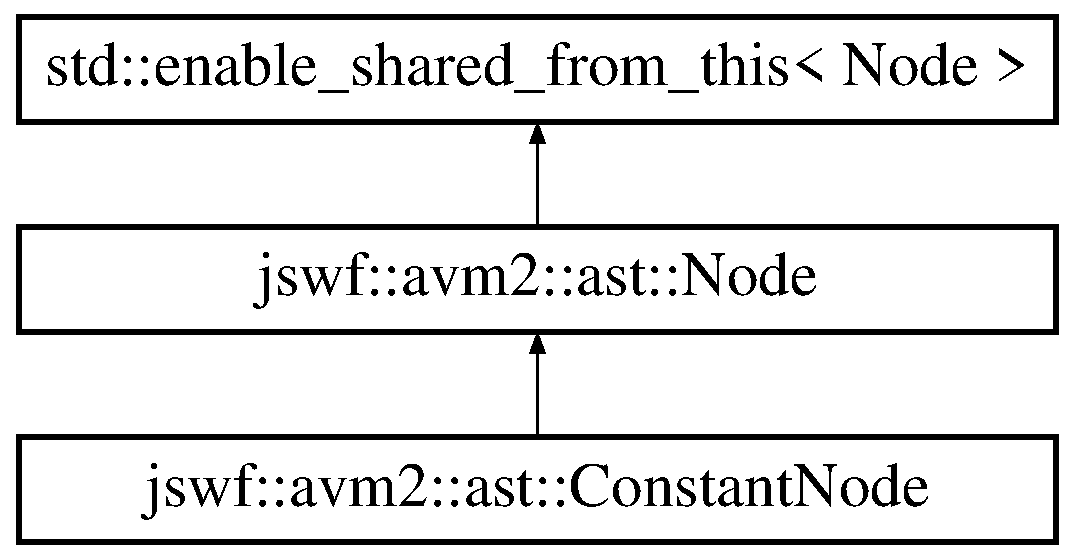
\includegraphics[height=3.000000cm]{classjswf_1_1avm2_1_1ast_1_1_constant_node}
\end{center}
\end{figure}
\subsection*{Public Member Functions}
\begin{DoxyCompactItemize}
\item 
\hypertarget{classjswf_1_1avm2_1_1ast_1_1_constant_node_ac38d4d91c7d76cf68b0f86580deb88f0}{{\bfseries Constant\+Node} (const std\+::string \&str)}\label{classjswf_1_1avm2_1_1ast_1_1_constant_node_ac38d4d91c7d76cf68b0f86580deb88f0}

\item 
\hypertarget{classjswf_1_1avm2_1_1ast_1_1_constant_node_a738a97d088ba21b6ba29d0fa9de2a6e3}{virtual std\+::string {\bfseries to\+String} ()}\label{classjswf_1_1avm2_1_1ast_1_1_constant_node_a738a97d088ba21b6ba29d0fa9de2a6e3}

\end{DoxyCompactItemize}
\subsection*{Public Attributes}
\begin{DoxyCompactItemize}
\item 
\hypertarget{classjswf_1_1avm2_1_1ast_1_1_constant_node_a27185ae5d7b462ac017527f5536b9cd4}{std\+::string {\bfseries value}}\label{classjswf_1_1avm2_1_1ast_1_1_constant_node_a27185ae5d7b462ac017527f5536b9cd4}

\end{DoxyCompactItemize}


The documentation for this class was generated from the following file\+:\begin{DoxyCompactItemize}
\item 
jswf/avm2/ast/Node.\+h\end{DoxyCompactItemize}

\hypertarget{structjswf_1_1avm2_1_1_constant_pool}{\section{jswf\+:\+:avm2\+:\+:Constant\+Pool Struct Reference}
\label{structjswf_1_1avm2_1_1_constant_pool}\index{jswf\+::avm2\+::\+Constant\+Pool@{jswf\+::avm2\+::\+Constant\+Pool}}
}
\subsection*{Classes}
\begin{DoxyCompactItemize}
\item 
class \hyperlink{classjswf_1_1avm2_1_1_constant_pool_1_1_set_u30}{Set\+U30}
\begin{DoxyCompactList}\small\item\em Extends std\+::vector$<$\+T$>$ to support set-\/like behavior. \end{DoxyCompactList}\end{DoxyCompactItemize}
\subsection*{Public Attributes}
\begin{DoxyCompactItemize}
\item 
\hypertarget{structjswf_1_1avm2_1_1_constant_pool_aab573ed0ddae6cc8a9e66ccb927fb46f}{\hyperlink{classjswf_1_1avm2_1_1_constant_pool_1_1_set_u30}{Set\+U30}$<$ \hyperlink{namespacejswf_a19b2a5980fe3b05994a2127a3c7e0521}{s32\+\_\+t} $>$ {\bfseries integers}}\label{structjswf_1_1avm2_1_1_constant_pool_aab573ed0ddae6cc8a9e66ccb927fb46f}

\item 
\hypertarget{structjswf_1_1avm2_1_1_constant_pool_a605cf0668e98e28d76797a4c6d699368}{\hyperlink{classjswf_1_1avm2_1_1_constant_pool_1_1_set_u30}{Set\+U30}$<$ \hyperlink{namespacejswf_ae68dd480b6437e9a20db7b004283a466}{u32\+\_\+t} $>$ {\bfseries uintegers}}\label{structjswf_1_1avm2_1_1_constant_pool_a605cf0668e98e28d76797a4c6d699368}

\item 
\hypertarget{structjswf_1_1avm2_1_1_constant_pool_a676c0a5a79c9e364979797a4bd9debfa}{\hyperlink{classjswf_1_1avm2_1_1_constant_pool_1_1_set_u30}{Set\+U30}$<$ \hyperlink{namespacejswf_acfbb3c7c9fbb807e233387995eb76a96}{d64\+\_\+t} $>$ {\bfseries doubles}}\label{structjswf_1_1avm2_1_1_constant_pool_a676c0a5a79c9e364979797a4bd9debfa}

\item 
\hypertarget{structjswf_1_1avm2_1_1_constant_pool_a27a70d2cfeb499e512c4fe444a5c0d55}{\hyperlink{classjswf_1_1avm2_1_1_constant_pool_1_1_set_u30}{Set\+U30}$<$ \hyperlink{namespacejswf_a755127d61081aa8af105eb800aa2c1ec}{string} $>$ {\bfseries strings}}\label{structjswf_1_1avm2_1_1_constant_pool_a27a70d2cfeb499e512c4fe444a5c0d55}

\item 
\hypertarget{structjswf_1_1avm2_1_1_constant_pool_a92b85d6fa727cb04267edced3b7ab8ab}{\hyperlink{classjswf_1_1avm2_1_1_constant_pool_1_1_set_u30}{Set\+U30}$<$ Namespace\+Ptr $>$ {\bfseries namespaces}}\label{structjswf_1_1avm2_1_1_constant_pool_a92b85d6fa727cb04267edced3b7ab8ab}

\item 
\hypertarget{structjswf_1_1avm2_1_1_constant_pool_a33af185abce905e790e4f5e6975b23b7}{\hyperlink{classjswf_1_1avm2_1_1_constant_pool_1_1_set_u30}{Set\+U30}$<$ Namespace\+Set\+Ptr $>$ {\bfseries namespace\+Sets}}\label{structjswf_1_1avm2_1_1_constant_pool_a33af185abce905e790e4f5e6975b23b7}

\item 
\hypertarget{structjswf_1_1avm2_1_1_constant_pool_a093544e8eca8f4b8aa6a2a84312d9587}{\hyperlink{classjswf_1_1avm2_1_1_constant_pool_1_1_set_u30}{Set\+U30}$<$ Multiname\+Ptr $>$ {\bfseries multinames}}\label{structjswf_1_1avm2_1_1_constant_pool_a093544e8eca8f4b8aa6a2a84312d9587}

\end{DoxyCompactItemize}


The documentation for this struct was generated from the following file\+:\begin{DoxyCompactItemize}
\item 
jswf/avm2/A\+B\+C\+File.\+h\end{DoxyCompactItemize}

\hypertarget{structjswf_1_1render_1_1_context}{\section{jswf\+:\+:render\+:\+:Context Struct Reference}
\label{structjswf_1_1render_1_1_context}\index{jswf\+::render\+::\+Context@{jswf\+::render\+::\+Context}}
}


{\ttfamily \#include $<$Render.\+h$>$}

\subsection*{Public Attributes}
\begin{DoxyCompactItemize}
\item 
\hypertarget{structjswf_1_1render_1_1_context_afe4f5780493a0e06b7f1814b99cb30e5}{uint16\+\_\+t {\bfseries w}}\label{structjswf_1_1render_1_1_context_afe4f5780493a0e06b7f1814b99cb30e5}

\item 
\hypertarget{structjswf_1_1render_1_1_context_a980b0157be571b58ec939d691067b2f8}{uint16\+\_\+t {\bfseries h}}\label{structjswf_1_1render_1_1_context_a980b0157be571b58ec939d691067b2f8}

\item 
\hypertarget{structjswf_1_1render_1_1_context_a0ac41bf5c33e320c9110b4b4e15e1965}{uint32\+\_\+t $\ast$ {\bfseries buffer}}\label{structjswf_1_1render_1_1_context_a0ac41bf5c33e320c9110b4b4e15e1965}

\item 
\hypertarget{structjswf_1_1render_1_1_context_a94c6275ef656062d820b00bee4635a4c}{uint32\+\_\+t $\ast$ {\bfseries clip} = N\+U\+L\+L}\label{structjswf_1_1render_1_1_context_a94c6275ef656062d820b00bee4635a4c}

\item 
\hypertarget{structjswf_1_1render_1_1_context_afe7d8b50188784d2509c1bc36c29db38}{\hyperlink{structjswf_1_1flash_1_1_matrix}{flash\+::\+Matrix} {\bfseries matrix}}\label{structjswf_1_1render_1_1_context_afe7d8b50188784d2509c1bc36c29db38}

\item 
\hypertarget{structjswf_1_1render_1_1_context_a4bb2f94db91982e512568032722fb19e}{\hyperlink{structjswf_1_1flash_1_1_color_transform}{flash\+::\+Color\+Transform} {\bfseries color\+Transform}}\label{structjswf_1_1render_1_1_context_a4bb2f94db91982e512568032722fb19e}

\item 
\hypertarget{structjswf_1_1render_1_1_context_aa5c663199a983f23d1fb56f18b6cc4af}{\hyperlink{classjswf_1_1flash_1_1_document}{flash\+::\+Document} $\ast$ {\bfseries document}}\label{structjswf_1_1render_1_1_context_aa5c663199a983f23d1fb56f18b6cc4af}

\end{DoxyCompactItemize}


\subsection{Detailed Description}
\begin{DoxyRefDesc}{Bug}
\item[\hyperlink{bug__bug000001}{Bug}]Lines not rendering. \end{DoxyRefDesc}


The documentation for this struct was generated from the following file\+:\begin{DoxyCompactItemize}
\item 
jswf/render/Render.\+h\end{DoxyCompactItemize}

\hypertarget{classjswf_1_1flash_1_1tags_1_1_define_button2_tag}{\section{jswf\+:\+:flash\+:\+:tags\+:\+:Define\+Button2\+Tag Class Reference}
\label{classjswf_1_1flash_1_1tags_1_1_define_button2_tag}\index{jswf\+::flash\+::tags\+::\+Define\+Button2\+Tag@{jswf\+::flash\+::tags\+::\+Define\+Button2\+Tag}}
}


Extends \hyperlink{classjswf_1_1flash_1_1tags_1_1_define_button_tag}{Define\+Button\+Tag} with support for {\ttfamily Track\+As\+Menu}.  




{\ttfamily \#include $<$Define\+Button2\+Tag.\+h$>$}

Inheritance diagram for jswf\+:\+:flash\+:\+:tags\+:\+:Define\+Button2\+Tag\+:\begin{figure}[H]
\begin{center}
\leavevmode
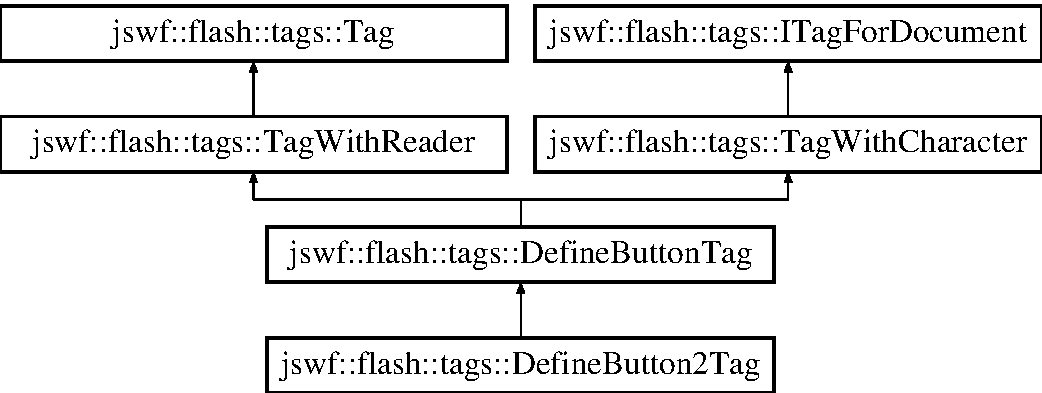
\includegraphics[height=4.000000cm]{classjswf_1_1flash_1_1tags_1_1_define_button2_tag}
\end{center}
\end{figure}
\subsection*{Public Member Functions}
\begin{DoxyCompactItemize}
\item 
\hypertarget{classjswf_1_1flash_1_1tags_1_1_define_button2_tag_ac7600948149376eb293d3064a93b5bf7}{{\bfseries Define\+Button2\+Tag} (tag\+\_\+type\+\_\+t t, std\+::string \&p)}\label{classjswf_1_1flash_1_1tags_1_1_define_button2_tag_ac7600948149376eb293d3064a93b5bf7}

\item 
\hypertarget{classjswf_1_1flash_1_1tags_1_1_define_button2_tag_ae8ae0893da19eab72e3ec3ec35048d98}{{\bfseries Define\+Button2\+Tag} (tag\+\_\+type\+\_\+t t, std\+::string \&p, bool)}\label{classjswf_1_1flash_1_1tags_1_1_define_button2_tag_ae8ae0893da19eab72e3ec3ec35048d98}

\end{DoxyCompactItemize}
\subsection*{Protected Member Functions}
\begin{DoxyCompactItemize}
\item 
virtual void \hyperlink{classjswf_1_1flash_1_1tags_1_1_define_button2_tag_a022b48db351f0e0113a1df52a941f717}{read\+Between} ()
\end{DoxyCompactItemize}
\subsection*{Additional Inherited Members}


\subsection{Detailed Description}
Extends \hyperlink{classjswf_1_1flash_1_1tags_1_1_define_button_tag}{Define\+Button\+Tag} with support for {\ttfamily Track\+As\+Menu}. 

\begin{DoxyRefDesc}{Todo}
\item[\hyperlink{todo__todo000014}{Todo}]\char`\"{}by allowing any state transition to trigger actions.\char`\"{}... what? \end{DoxyRefDesc}


\subsection{Member Function Documentation}
\hypertarget{classjswf_1_1flash_1_1tags_1_1_define_button2_tag_a022b48db351f0e0113a1df52a941f717}{\index{jswf\+::flash\+::tags\+::\+Define\+Button2\+Tag@{jswf\+::flash\+::tags\+::\+Define\+Button2\+Tag}!read\+Between@{read\+Between}}
\index{read\+Between@{read\+Between}!jswf\+::flash\+::tags\+::\+Define\+Button2\+Tag@{jswf\+::flash\+::tags\+::\+Define\+Button2\+Tag}}
\subsubsection[{read\+Between}]{\setlength{\rightskip}{0pt plus 5cm}virtual void jswf\+::flash\+::tags\+::\+Define\+Button2\+Tag\+::read\+Between (
\begin{DoxyParamCaption}
{}
\end{DoxyParamCaption}
)\hspace{0.3cm}{\ttfamily [inline]}, {\ttfamily [protected]}, {\ttfamily [virtual]}}}\label{classjswf_1_1flash_1_1tags_1_1_define_button2_tag_a022b48db351f0e0113a1df52a941f717}
\begin{DoxySeeAlso}{See also}
\hyperlink{classjswf_1_1flash_1_1tags_1_1_define_shape_tag_a07ce111b115f578e0581b614dcdbd271}{Define\+Shape\+Tag\+::read\+Between} 
\end{DoxySeeAlso}


Reimplemented from \hyperlink{classjswf_1_1flash_1_1tags_1_1_define_button_tag_ab984c03a3deccd5619922753ef43cff2}{jswf\+::flash\+::tags\+::\+Define\+Button\+Tag}.



The documentation for this class was generated from the following file\+:\begin{DoxyCompactItemize}
\item 
jswf/flash/tags/Define\+Button2\+Tag.\+h\end{DoxyCompactItemize}

\hypertarget{classjswf_1_1flash_1_1tags_1_1_define_button_tag}{\section{jswf\+:\+:flash\+:\+:tags\+:\+:Define\+Button\+Tag Class Reference}
\label{classjswf_1_1flash_1_1tags_1_1_define_button_tag}\index{jswf\+::flash\+::tags\+::\+Define\+Button\+Tag@{jswf\+::flash\+::tags\+::\+Define\+Button\+Tag}}
}


Parses a {\ttfamily B\+U\+T\+T\+O\+N} record that is to be added to the document's {\ttfamily D\+I\+C\+T\+I\+O\+N\+A\+R\+Y}.  




{\ttfamily \#include $<$Define\+Button\+Tag.\+h$>$}

Inheritance diagram for jswf\+:\+:flash\+:\+:tags\+:\+:Define\+Button\+Tag\+:\begin{figure}[H]
\begin{center}
\leavevmode
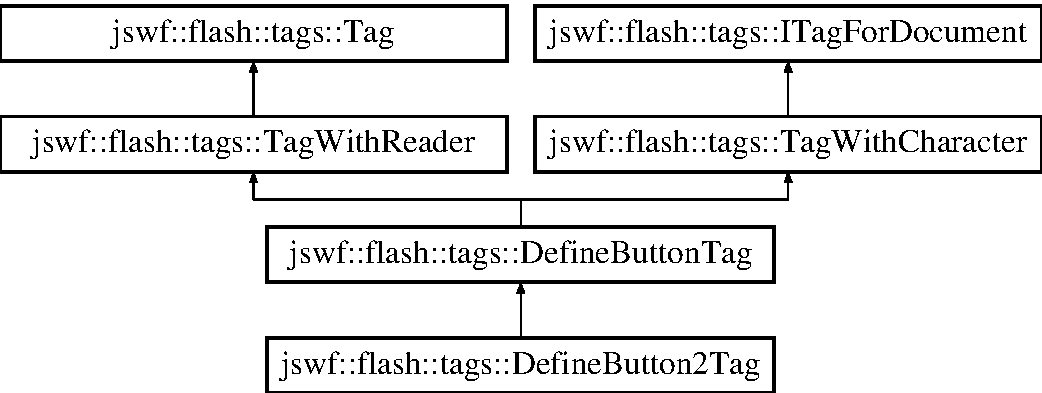
\includegraphics[height=4.000000cm]{classjswf_1_1flash_1_1tags_1_1_define_button_tag}
\end{center}
\end{figure}
\subsection*{Public Member Functions}
\begin{DoxyCompactItemize}
\item 
\hypertarget{classjswf_1_1flash_1_1tags_1_1_define_button_tag_aeb0d83077ba8f9d6267b64732f7f8dc8}{{\bfseries Define\+Button\+Tag} (tag\+\_\+type\+\_\+t t, std\+::string \&p)}\label{classjswf_1_1flash_1_1tags_1_1_define_button_tag_aeb0d83077ba8f9d6267b64732f7f8dc8}

\item 
\hypertarget{classjswf_1_1flash_1_1tags_1_1_define_button_tag_a2595f43f91fab3e3f328cbb6778cf4e0}{{\bfseries Define\+Button\+Tag} (tag\+\_\+type\+\_\+t t, std\+::string \&p, bool)}\label{classjswf_1_1flash_1_1tags_1_1_define_button_tag_a2595f43f91fab3e3f328cbb6778cf4e0}

\end{DoxyCompactItemize}
\subsection*{Public Attributes}
\begin{DoxyCompactItemize}
\item 
\hypertarget{classjswf_1_1flash_1_1tags_1_1_define_button_tag_aaefc1f3509d742c22095608b15a99ab5}{\hyperlink{classjswf_1_1flash_1_1_button}{Button} $\ast$ \hyperlink{classjswf_1_1flash_1_1tags_1_1_define_button_tag_aaefc1f3509d742c22095608b15a99ab5}{button}}\label{classjswf_1_1flash_1_1tags_1_1_define_button_tag_aaefc1f3509d742c22095608b15a99ab5}

\begin{DoxyCompactList}\small\item\em The button described by this tag. \end{DoxyCompactList}\end{DoxyCompactItemize}
\subsection*{Protected Member Functions}
\begin{DoxyCompactItemize}
\item 
bool \hyperlink{classjswf_1_1flash_1_1tags_1_1_define_button_tag_a7e9e4408daecaf9baabaffcce193799f}{read\+Button\+Record} ()
\begin{DoxyCompactList}\small\item\em Reads a 'B\+U\+T\+T\+O\+N\+R\+E\+C\+O\+R\+D'. \end{DoxyCompactList}\item 
virtual void \hyperlink{classjswf_1_1flash_1_1tags_1_1_define_button_tag_ab984c03a3deccd5619922753ef43cff2}{read\+Between} ()
\item 
void \hyperlink{classjswf_1_1flash_1_1tags_1_1_define_button_tag_ae358498c775dbe0271fae6d9b5a44643}{read} ()
\begin{DoxyCompactList}\small\item\em Instantiates button and parses the payload. \end{DoxyCompactList}\end{DoxyCompactItemize}


\subsection{Detailed Description}
Parses a {\ttfamily B\+U\+T\+T\+O\+N} record that is to be added to the document's {\ttfamily D\+I\+C\+T\+I\+O\+N\+A\+R\+Y}. 

\subsection{Member Function Documentation}
\hypertarget{classjswf_1_1flash_1_1tags_1_1_define_button_tag_ae358498c775dbe0271fae6d9b5a44643}{\index{jswf\+::flash\+::tags\+::\+Define\+Button\+Tag@{jswf\+::flash\+::tags\+::\+Define\+Button\+Tag}!read@{read}}
\index{read@{read}!jswf\+::flash\+::tags\+::\+Define\+Button\+Tag@{jswf\+::flash\+::tags\+::\+Define\+Button\+Tag}}
\subsubsection[{read}]{\setlength{\rightskip}{0pt plus 5cm}void jswf\+::flash\+::tags\+::\+Define\+Button\+Tag\+::read (
\begin{DoxyParamCaption}
{}
\end{DoxyParamCaption}
)\hspace{0.3cm}{\ttfamily [inline]}, {\ttfamily [protected]}}}\label{classjswf_1_1flash_1_1tags_1_1_define_button_tag_ae358498c775dbe0271fae6d9b5a44643}


Instantiates button and parses the payload. 

\begin{DoxySeeAlso}{See also}
\hyperlink{classjswf_1_1flash_1_1tags_1_1_define_button_tag_ab984c03a3deccd5619922753ef43cff2}{read\+Between} 

\hyperlink{classjswf_1_1flash_1_1tags_1_1_define_button_tag_a7e9e4408daecaf9baabaffcce193799f}{read\+Button\+Record} 
\end{DoxySeeAlso}
\hypertarget{classjswf_1_1flash_1_1tags_1_1_define_button_tag_ab984c03a3deccd5619922753ef43cff2}{\index{jswf\+::flash\+::tags\+::\+Define\+Button\+Tag@{jswf\+::flash\+::tags\+::\+Define\+Button\+Tag}!read\+Between@{read\+Between}}
\index{read\+Between@{read\+Between}!jswf\+::flash\+::tags\+::\+Define\+Button\+Tag@{jswf\+::flash\+::tags\+::\+Define\+Button\+Tag}}
\subsubsection[{read\+Between}]{\setlength{\rightskip}{0pt plus 5cm}virtual void jswf\+::flash\+::tags\+::\+Define\+Button\+Tag\+::read\+Between (
\begin{DoxyParamCaption}
{}
\end{DoxyParamCaption}
)\hspace{0.3cm}{\ttfamily [inline]}, {\ttfamily [protected]}, {\ttfamily [virtual]}}}\label{classjswf_1_1flash_1_1tags_1_1_define_button_tag_ab984c03a3deccd5619922753ef43cff2}
\begin{DoxySeeAlso}{See also}
\hyperlink{classjswf_1_1flash_1_1tags_1_1_define_shape_tag_a07ce111b115f578e0581b614dcdbd271}{Define\+Shape\+Tag\+::read\+Between} 
\end{DoxySeeAlso}


Reimplemented in \hyperlink{classjswf_1_1flash_1_1tags_1_1_define_button2_tag_a022b48db351f0e0113a1df52a941f717}{jswf\+::flash\+::tags\+::\+Define\+Button2\+Tag}.

\hypertarget{classjswf_1_1flash_1_1tags_1_1_define_button_tag_a7e9e4408daecaf9baabaffcce193799f}{\index{jswf\+::flash\+::tags\+::\+Define\+Button\+Tag@{jswf\+::flash\+::tags\+::\+Define\+Button\+Tag}!read\+Button\+Record@{read\+Button\+Record}}
\index{read\+Button\+Record@{read\+Button\+Record}!jswf\+::flash\+::tags\+::\+Define\+Button\+Tag@{jswf\+::flash\+::tags\+::\+Define\+Button\+Tag}}
\subsubsection[{read\+Button\+Record}]{\setlength{\rightskip}{0pt plus 5cm}bool jswf\+::flash\+::tags\+::\+Define\+Button\+Tag\+::read\+Button\+Record (
\begin{DoxyParamCaption}
{}
\end{DoxyParamCaption}
)\hspace{0.3cm}{\ttfamily [inline]}, {\ttfamily [protected]}}}\label{classjswf_1_1flash_1_1tags_1_1_define_button_tag_a7e9e4408daecaf9baabaffcce193799f}


Reads a 'B\+U\+T\+T\+O\+N\+R\+E\+C\+O\+R\+D'. 

The changes to the frame are applied to button. \begin{DoxyReturn}{Returns}
{\ttfamily true} if further records follow, {\ttfamily false} if this was the last record. 
\end{DoxyReturn}

\begin{DoxyExceptions}{Exceptions}
{\em (\+T\+O\+D\+O)} & if the reserved field was non-\/zero. \\
\hline
\end{DoxyExceptions}
\begin{DoxySeeAlso}{See also}
\hyperlink{classjswf_1_1flash_1_1tags_1_1_define_button_tag_ae358498c775dbe0271fae6d9b5a44643}{read} 
\end{DoxySeeAlso}


The documentation for this class was generated from the following file\+:\begin{DoxyCompactItemize}
\item 
jswf/flash/tags/Define\+Button\+Tag.\+h\end{DoxyCompactItemize}

\hypertarget{classjswf_1_1flash_1_1tags_1_1_define_scene_and_frame_label_data_tag}{\section{jswf\+:\+:flash\+:\+:tags\+:\+:Define\+Scene\+And\+Frame\+Label\+Data\+Tag Class Reference}
\label{classjswf_1_1flash_1_1tags_1_1_define_scene_and_frame_label_data_tag}\index{jswf\+::flash\+::tags\+::\+Define\+Scene\+And\+Frame\+Label\+Data\+Tag@{jswf\+::flash\+::tags\+::\+Define\+Scene\+And\+Frame\+Label\+Data\+Tag}}
}


Carries instances of \hyperlink{structjswf_1_1flash_1_1_scene}{Scene} and instances of \hyperlink{structjswf_1_1flash_1_1_frame_label}{Frame\+Label}.  




{\ttfamily \#include $<$Define\+Scene\+And\+Frame\+Label\+Data\+Tag.\+h$>$}

Inheritance diagram for jswf\+:\+:flash\+:\+:tags\+:\+:Define\+Scene\+And\+Frame\+Label\+Data\+Tag\+:\begin{figure}[H]
\begin{center}
\leavevmode
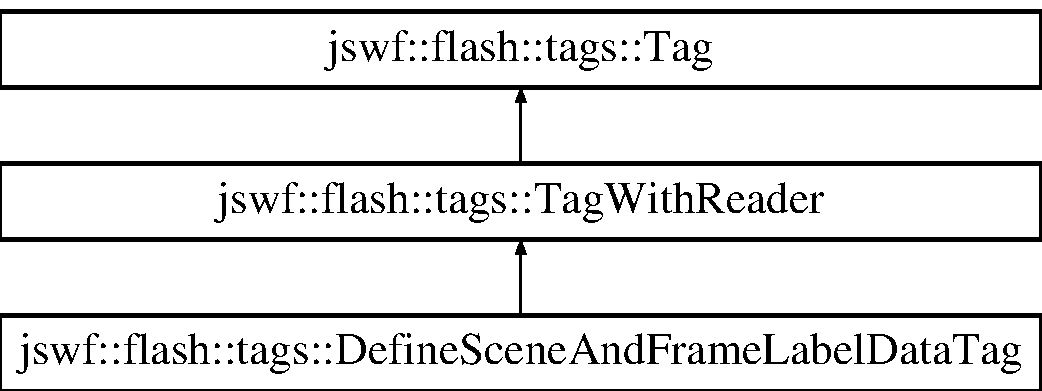
\includegraphics[height=3.000000cm]{classjswf_1_1flash_1_1tags_1_1_define_scene_and_frame_label_data_tag}
\end{center}
\end{figure}
\subsection*{Public Member Functions}
\begin{DoxyCompactItemize}
\item 
\hypertarget{classjswf_1_1flash_1_1tags_1_1_define_scene_and_frame_label_data_tag_a047c7ef3c94ed3149952d2e0a8b84c44}{{\bfseries Define\+Scene\+And\+Frame\+Label\+Data\+Tag} (tag\+\_\+type\+\_\+t t, std\+::string \&p)}\label{classjswf_1_1flash_1_1tags_1_1_define_scene_and_frame_label_data_tag_a047c7ef3c94ed3149952d2e0a8b84c44}

\end{DoxyCompactItemize}
\subsection*{Public Attributes}
\begin{DoxyCompactItemize}
\item 
\hypertarget{classjswf_1_1flash_1_1tags_1_1_define_scene_and_frame_label_data_tag_ab9441381394fa591ec29756c8a4d97f6}{std\+::vector$<$ \hyperlink{structjswf_1_1flash_1_1_scene}{Scene} $>$ \hyperlink{classjswf_1_1flash_1_1tags_1_1_define_scene_and_frame_label_data_tag_ab9441381394fa591ec29756c8a4d97f6}{scenes}}\label{classjswf_1_1flash_1_1tags_1_1_define_scene_and_frame_label_data_tag_ab9441381394fa591ec29756c8a4d97f6}

\begin{DoxyCompactList}\small\item\em The instances of \hyperlink{structjswf_1_1flash_1_1_scene}{Scene} that are described by this tag. \end{DoxyCompactList}\item 
\hypertarget{classjswf_1_1flash_1_1tags_1_1_define_scene_and_frame_label_data_tag_a4419863b88233717dc8c95d99fc0dfa1}{std\+::vector$<$ \hyperlink{structjswf_1_1flash_1_1_frame_label}{Frame\+Label} $>$ \hyperlink{classjswf_1_1flash_1_1tags_1_1_define_scene_and_frame_label_data_tag_a4419863b88233717dc8c95d99fc0dfa1}{frame\+Labels}}\label{classjswf_1_1flash_1_1tags_1_1_define_scene_and_frame_label_data_tag_a4419863b88233717dc8c95d99fc0dfa1}

\begin{DoxyCompactList}\small\item\em The instances of \hyperlink{structjswf_1_1flash_1_1_frame_label}{Frame\+Label} that are described by this tag. \end{DoxyCompactList}\end{DoxyCompactItemize}


\subsection{Detailed Description}
Carries instances of \hyperlink{structjswf_1_1flash_1_1_scene}{Scene} and instances of \hyperlink{structjswf_1_1flash_1_1_frame_label}{Frame\+Label}. 

The documentation for this class was generated from the following file\+:\begin{DoxyCompactItemize}
\item 
jswf/flash/tags/Define\+Scene\+And\+Frame\+Label\+Data\+Tag.\+h\end{DoxyCompactItemize}

\hypertarget{classjswf_1_1flash_1_1tags_1_1_define_shape2_tag}{\section{jswf\+:\+:flash\+:\+:tags\+:\+:Define\+Shape2\+Tag Class Reference}
\label{classjswf_1_1flash_1_1tags_1_1_define_shape2_tag}\index{jswf\+::flash\+::tags\+::\+Define\+Shape2\+Tag@{jswf\+::flash\+::tags\+::\+Define\+Shape2\+Tag}}
}


Extends \hyperlink{classjswf_1_1flash_1_1tags_1_1_define_shape_tag}{Define\+Shape\+Tag} with support for up to 65534 (0xfffe) elements for {\ttfamily Fill\+Style\+Array} and {\ttfamily Line\+Style\+Array}.  




{\ttfamily \#include $<$Define\+Shape2\+Tag.\+h$>$}

Inheritance diagram for jswf\+:\+:flash\+:\+:tags\+:\+:Define\+Shape2\+Tag\+:\begin{figure}[H]
\begin{center}
\leavevmode
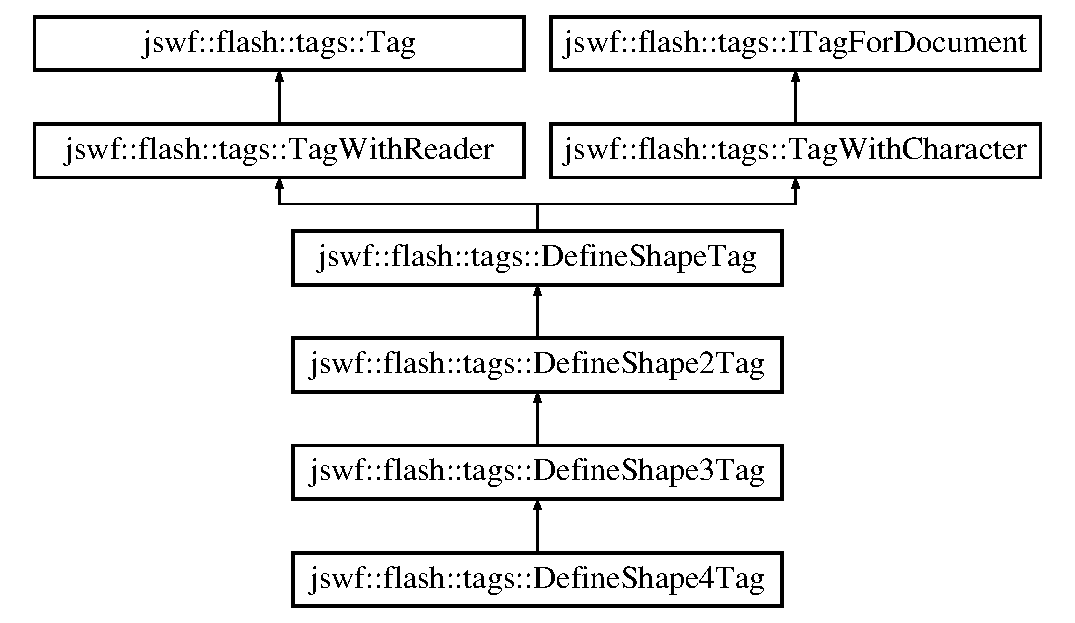
\includegraphics[height=6.000000cm]{classjswf_1_1flash_1_1tags_1_1_define_shape2_tag}
\end{center}
\end{figure}
\subsection*{Public Member Functions}
\begin{DoxyCompactItemize}
\item 
\hypertarget{classjswf_1_1flash_1_1tags_1_1_define_shape2_tag_a35e1656b28c806bc2d3486fa2023d60f}{{\bfseries Define\+Shape2\+Tag} (tag\+\_\+type\+\_\+t t, std\+::string \&p)}\label{classjswf_1_1flash_1_1tags_1_1_define_shape2_tag_a35e1656b28c806bc2d3486fa2023d60f}

\item 
\hypertarget{classjswf_1_1flash_1_1tags_1_1_define_shape2_tag_a742988a0442ec623d960070026f5ab22}{{\bfseries Define\+Shape2\+Tag} (tag\+\_\+type\+\_\+t t, std\+::string \&p, bool)}\label{classjswf_1_1flash_1_1tags_1_1_define_shape2_tag_a742988a0442ec623d960070026f5ab22}

\end{DoxyCompactItemize}
\subsection*{Protected Member Functions}
\begin{DoxyCompactItemize}
\item 
\hypertarget{classjswf_1_1flash_1_1tags_1_1_define_shape2_tag_a6e952275a3ad934e55f4ea481fe2f8e5}{virtual void \hyperlink{classjswf_1_1flash_1_1tags_1_1_define_shape2_tag_a6e952275a3ad934e55f4ea481fe2f8e5}{read\+Between} ()}\label{classjswf_1_1flash_1_1tags_1_1_define_shape2_tag_a6e952275a3ad934e55f4ea481fe2f8e5}

\begin{DoxyCompactList}\small\item\em Implemented by subclasses to perform reads between 'Bounds' and 'Fill\+Style\+Array'. \end{DoxyCompactList}\item 
virtual uint16\+\_\+t \hyperlink{classjswf_1_1flash_1_1tags_1_1_define_shape2_tag_a1a6b796a542d30359ee662b68f13c208}{read\+Array\+Count} ()
\begin{DoxyCompactList}\small\item\em Reads an array count from the payload stream. \end{DoxyCompactList}\end{DoxyCompactItemize}
\subsection*{Additional Inherited Members}


\subsection{Detailed Description}
Extends \hyperlink{classjswf_1_1flash_1_1tags_1_1_define_shape_tag}{Define\+Shape\+Tag} with support for up to 65534 (0xfffe) elements for {\ttfamily Fill\+Style\+Array} and {\ttfamily Line\+Style\+Array}. 

\subsection{Member Function Documentation}
\hypertarget{classjswf_1_1flash_1_1tags_1_1_define_shape2_tag_a1a6b796a542d30359ee662b68f13c208}{\index{jswf\+::flash\+::tags\+::\+Define\+Shape2\+Tag@{jswf\+::flash\+::tags\+::\+Define\+Shape2\+Tag}!read\+Array\+Count@{read\+Array\+Count}}
\index{read\+Array\+Count@{read\+Array\+Count}!jswf\+::flash\+::tags\+::\+Define\+Shape2\+Tag@{jswf\+::flash\+::tags\+::\+Define\+Shape2\+Tag}}
\subsubsection[{read\+Array\+Count}]{\setlength{\rightskip}{0pt plus 5cm}virtual uint16\+\_\+t jswf\+::flash\+::tags\+::\+Define\+Shape2\+Tag\+::read\+Array\+Count (
\begin{DoxyParamCaption}
{}
\end{DoxyParamCaption}
)\hspace{0.3cm}{\ttfamily [inline]}, {\ttfamily [protected]}, {\ttfamily [virtual]}}}\label{classjswf_1_1flash_1_1tags_1_1_define_shape2_tag_a1a6b796a542d30359ee662b68f13c208}


Reads an array count from the payload stream. 

Subclasses can override this to add support for longer arrays. 
\begin{DoxyExceptions}{Exceptions}
{\em (\+T\+O\+D\+O)} & Exception\+Class when count == 0xff \\
\hline
\end{DoxyExceptions}
\begin{DoxyReturn}{Returns}
The count in \mbox{[}0;0xff) 
\end{DoxyReturn}
\begin{DoxySeeAlso}{See also}
\hyperlink{classjswf_1_1flash_1_1tags_1_1_define_shape_tag_ab15f7758c79bbb08f1804eebcb7488da}{read\+Line\+Style\+Array} 

\hyperlink{classjswf_1_1flash_1_1tags_1_1_define_shape_tag_a8688b9a3f2873e816a16e5450e4df167}{read\+Fill\+Style\+Array} 
\end{DoxySeeAlso}
$<$\begin{DoxyRefDesc}{Todo}
\item[\hyperlink{todo__todo000015}{Todo}]\hyperlink{classjswf_1_1flash_1_1_document}{Document} this. Especially throw. \end{DoxyRefDesc}


Reimplemented from \hyperlink{classjswf_1_1flash_1_1tags_1_1_define_shape_tag_a46f74909f7c7c63f5e9663a2465adc18}{jswf\+::flash\+::tags\+::\+Define\+Shape\+Tag}.



The documentation for this class was generated from the following file\+:\begin{DoxyCompactItemize}
\item 
jswf/flash/tags/Define\+Shape2\+Tag.\+h\end{DoxyCompactItemize}

\hypertarget{classjswf_1_1flash_1_1tags_1_1_define_shape3_tag}{\section{jswf\+:\+:flash\+:\+:tags\+:\+:Define\+Shape3\+Tag Class Reference}
\label{classjswf_1_1flash_1_1tags_1_1_define_shape3_tag}\index{jswf\+::flash\+::tags\+::\+Define\+Shape3\+Tag@{jswf\+::flash\+::tags\+::\+Define\+Shape3\+Tag}}
}


Extends \hyperlink{classjswf_1_1flash_1_1tags_1_1_define_shape2_tag}{Define\+Shape2\+Tag} with support for transparency in colors by using \hyperlink{classjswf_1_1flash_1_1_reader_a2c89e5f540d698d4d4fc4dc983dcf81c}{Reader\+::read\+R\+G\+B\+A} instead of \hyperlink{classjswf_1_1flash_1_1_reader_abba53a3337f589e3641681c2251e4d8d}{Reader\+::read\+R\+G\+B} .  




{\ttfamily \#include $<$Define\+Shape3\+Tag.\+h$>$}

Inheritance diagram for jswf\+:\+:flash\+:\+:tags\+:\+:Define\+Shape3\+Tag\+:\begin{figure}[H]
\begin{center}
\leavevmode
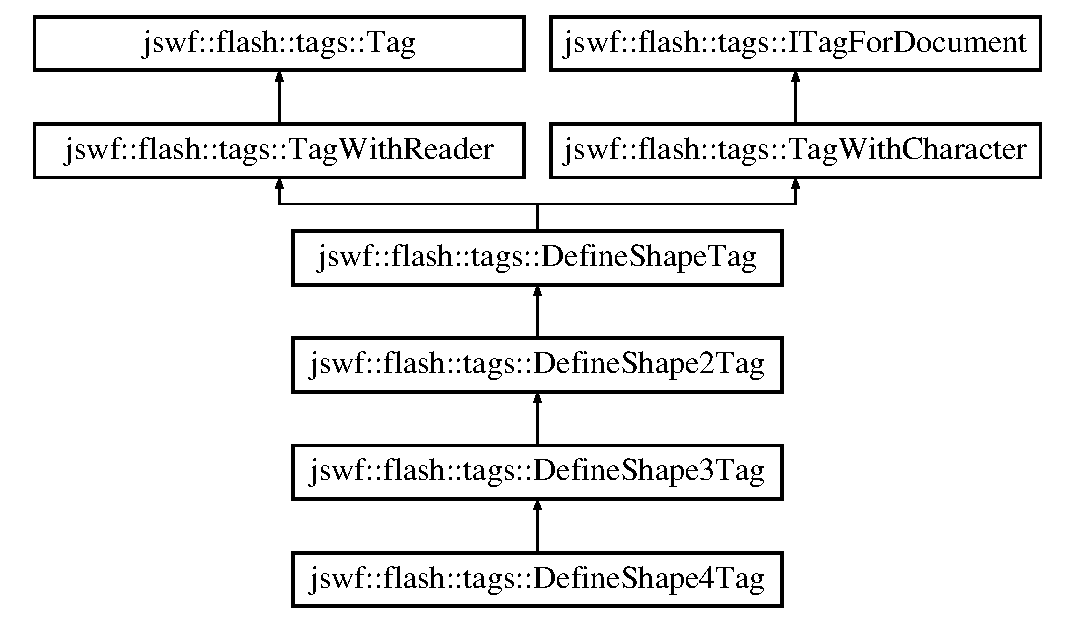
\includegraphics[height=6.000000cm]{classjswf_1_1flash_1_1tags_1_1_define_shape3_tag}
\end{center}
\end{figure}
\subsection*{Public Member Functions}
\begin{DoxyCompactItemize}
\item 
\hypertarget{classjswf_1_1flash_1_1tags_1_1_define_shape3_tag_ace71312c7aba7d88c3da2c122e7f9320}{{\bfseries Define\+Shape3\+Tag} (tag\+\_\+type\+\_\+t t, std\+::string \&p)}\label{classjswf_1_1flash_1_1tags_1_1_define_shape3_tag_ace71312c7aba7d88c3da2c122e7f9320}

\item 
\hypertarget{classjswf_1_1flash_1_1tags_1_1_define_shape3_tag_aa72e1084cb0052dec2b23a228db0d063}{{\bfseries Define\+Shape3\+Tag} (tag\+\_\+type\+\_\+t t, std\+::string \&p, bool)}\label{classjswf_1_1flash_1_1tags_1_1_define_shape3_tag_aa72e1084cb0052dec2b23a228db0d063}

\end{DoxyCompactItemize}
\subsection*{Protected Member Functions}
\begin{DoxyCompactItemize}
\item 
\hypertarget{classjswf_1_1flash_1_1tags_1_1_define_shape3_tag_a14b7e7770473f51a1658e712d968552c}{virtual void \hyperlink{classjswf_1_1flash_1_1tags_1_1_define_shape3_tag_a14b7e7770473f51a1658e712d968552c}{read\+Between} ()}\label{classjswf_1_1flash_1_1tags_1_1_define_shape3_tag_a14b7e7770473f51a1658e712d968552c}

\begin{DoxyCompactList}\small\item\em Implemented by subclasses to perform reads between 'Bounds' and 'Fill\+Style\+Array'. \end{DoxyCompactList}\item 
virtual void \hyperlink{classjswf_1_1flash_1_1tags_1_1_define_shape3_tag_a23bdaf9f98d600edbc0222c3ba4edc39}{read\+Color} (\hyperlink{structjswf_1_1flash_1_1_r_g_b_a}{R\+G\+B\+A} \&rgba)
\begin{DoxyCompactList}\small\item\em Reads a color from the payload stream. \end{DoxyCompactList}\end{DoxyCompactItemize}
\subsection*{Additional Inherited Members}


\subsection{Detailed Description}
Extends \hyperlink{classjswf_1_1flash_1_1tags_1_1_define_shape2_tag}{Define\+Shape2\+Tag} with support for transparency in colors by using \hyperlink{classjswf_1_1flash_1_1_reader_a2c89e5f540d698d4d4fc4dc983dcf81c}{Reader\+::read\+R\+G\+B\+A} instead of \hyperlink{classjswf_1_1flash_1_1_reader_abba53a3337f589e3641681c2251e4d8d}{Reader\+::read\+R\+G\+B} . 

\subsection{Member Function Documentation}
\hypertarget{classjswf_1_1flash_1_1tags_1_1_define_shape3_tag_a23bdaf9f98d600edbc0222c3ba4edc39}{\index{jswf\+::flash\+::tags\+::\+Define\+Shape3\+Tag@{jswf\+::flash\+::tags\+::\+Define\+Shape3\+Tag}!read\+Color@{read\+Color}}
\index{read\+Color@{read\+Color}!jswf\+::flash\+::tags\+::\+Define\+Shape3\+Tag@{jswf\+::flash\+::tags\+::\+Define\+Shape3\+Tag}}
\subsubsection[{read\+Color}]{\setlength{\rightskip}{0pt plus 5cm}virtual void jswf\+::flash\+::tags\+::\+Define\+Shape3\+Tag\+::read\+Color (
\begin{DoxyParamCaption}
\item[{{\bf R\+G\+B\+A} \&}]{rgba}
\end{DoxyParamCaption}
)\hspace{0.3cm}{\ttfamily [inline]}, {\ttfamily [protected]}, {\ttfamily [virtual]}}}\label{classjswf_1_1flash_1_1tags_1_1_define_shape3_tag_a23bdaf9f98d600edbc0222c3ba4edc39}


Reads a color from the payload stream. 

Subclasses can override this to add support for other color schemes (e. G. \hyperlink{structjswf_1_1flash_1_1_r_g_b_a}{R\+G\+B\+A}) 
\begin{DoxyParams}[1]{Parameters}
\mbox{\tt out}  & {\em rgba} & The R\+G\+B\+A-\/field to read into. \\
\hline
\end{DoxyParams}
\begin{DoxySeeAlso}{See also}
\hyperlink{classjswf_1_1flash_1_1tags_1_1_define_shape_tag_a4608b4e2716301637136fbbd1c5040ab}{read\+Fill\+Style} 

\hyperlink{classjswf_1_1flash_1_1tags_1_1_define_shape_tag_aecc1cc8ae869cd1bce8ec793c4c8124e}{read\+Line\+Style} 
\end{DoxySeeAlso}


Reimplemented from \hyperlink{classjswf_1_1flash_1_1tags_1_1_define_shape_tag_ad6886a89c251b532eecd1edf306943c1}{jswf\+::flash\+::tags\+::\+Define\+Shape\+Tag}.



The documentation for this class was generated from the following file\+:\begin{DoxyCompactItemize}
\item 
jswf/flash/tags/Define\+Shape3\+Tag.\+h\end{DoxyCompactItemize}

\hypertarget{classjswf_1_1flash_1_1tags_1_1_define_shape4_tag}{\section{jswf\+:\+:flash\+:\+:tags\+:\+:Define\+Shape4\+Tag Class Reference}
\label{classjswf_1_1flash_1_1tags_1_1_define_shape4_tag}\index{jswf\+::flash\+::tags\+::\+Define\+Shape4\+Tag@{jswf\+::flash\+::tags\+::\+Define\+Shape4\+Tag}}
}


Extends \hyperlink{classjswf_1_1flash_1_1tags_1_1_define_shape3_tag}{Define\+Shape3\+Tag} with support for {\ttfamily L\+I\+N\+E\+S\+T\+Y\+L\+E2}.  




{\ttfamily \#include $<$Define\+Shape4\+Tag.\+h$>$}

Inheritance diagram for jswf\+:\+:flash\+:\+:tags\+:\+:Define\+Shape4\+Tag\+:\begin{figure}[H]
\begin{center}
\leavevmode
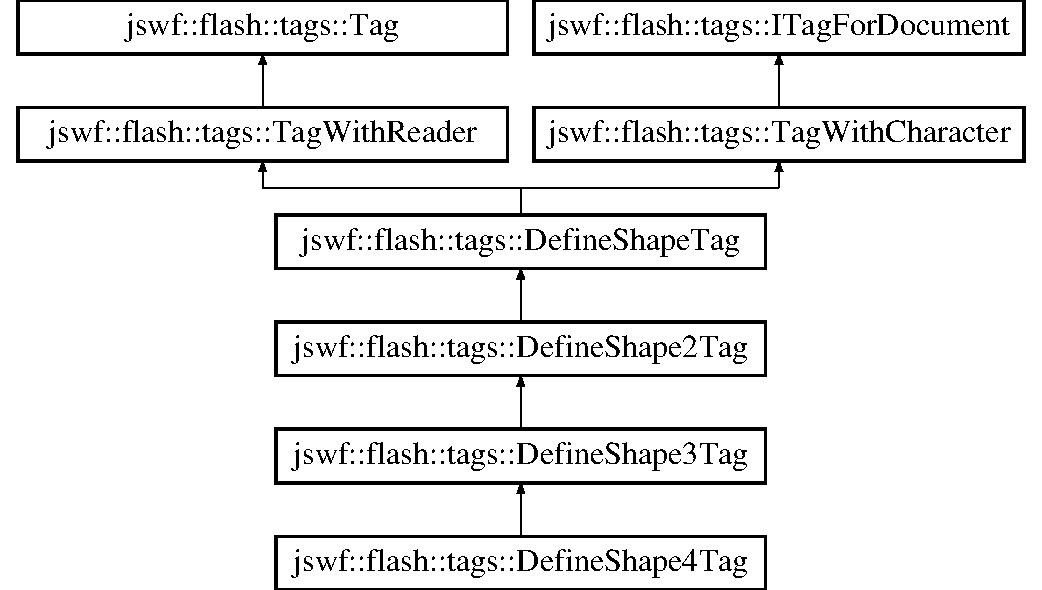
\includegraphics[height=6.000000cm]{classjswf_1_1flash_1_1tags_1_1_define_shape4_tag}
\end{center}
\end{figure}
\subsection*{Public Member Functions}
\begin{DoxyCompactItemize}
\item 
\hypertarget{classjswf_1_1flash_1_1tags_1_1_define_shape4_tag_a565066d2321f8567bb7930c5cb5b1c8e}{{\bfseries Define\+Shape4\+Tag} (tag\+\_\+type\+\_\+t t, std\+::string \&p)}\label{classjswf_1_1flash_1_1tags_1_1_define_shape4_tag_a565066d2321f8567bb7930c5cb5b1c8e}

\end{DoxyCompactItemize}
\subsection*{Additional Inherited Members}


\subsection{Detailed Description}
Extends \hyperlink{classjswf_1_1flash_1_1tags_1_1_define_shape3_tag}{Define\+Shape3\+Tag} with support for {\ttfamily L\+I\+N\+E\+S\+T\+Y\+L\+E2}. 

The documentation for this class was generated from the following file\+:\begin{DoxyCompactItemize}
\item 
jswf/flash/tags/Define\+Shape4\+Tag.\+h\end{DoxyCompactItemize}

\hypertarget{classjswf_1_1flash_1_1tags_1_1_define_shape_tag}{\section{jswf\+:\+:flash\+:\+:tags\+:\+:Define\+Shape\+Tag Class Reference}
\label{classjswf_1_1flash_1_1tags_1_1_define_shape_tag}\index{jswf\+::flash\+::tags\+::\+Define\+Shape\+Tag@{jswf\+::flash\+::tags\+::\+Define\+Shape\+Tag}}
}


Parses a {\ttfamily S\+H\+A\+P\+E} record that is to be added to the document's {\ttfamily D\+I\+C\+T\+I\+O\+N\+A\+R\+Y}.  




{\ttfamily \#include $<$Define\+Shape\+Tag.\+h$>$}

Inheritance diagram for jswf\+:\+:flash\+:\+:tags\+:\+:Define\+Shape\+Tag\+:\begin{figure}[H]
\begin{center}
\leavevmode
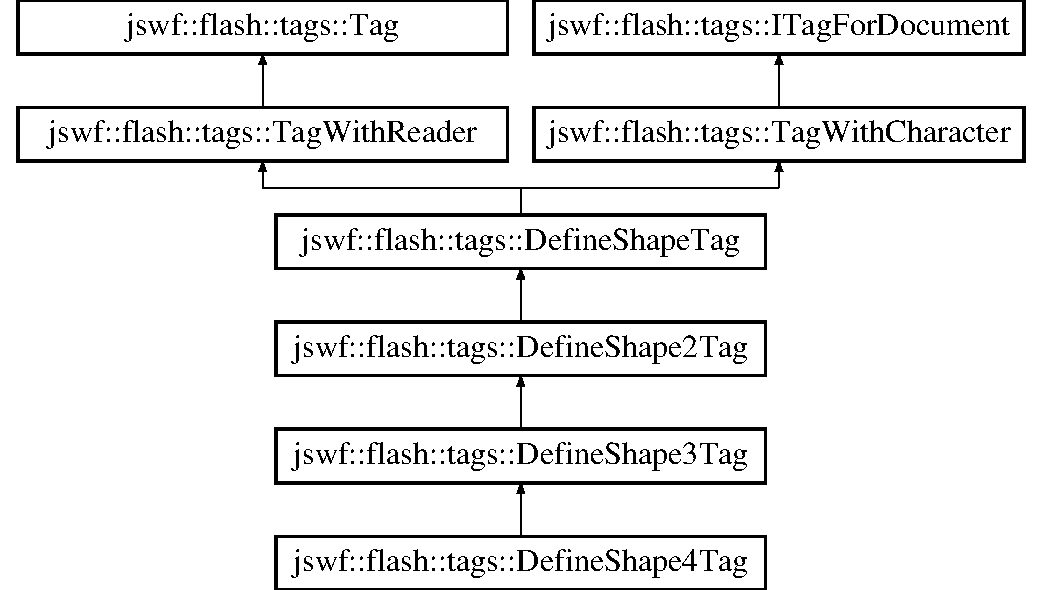
\includegraphics[height=6.000000cm]{classjswf_1_1flash_1_1tags_1_1_define_shape_tag}
\end{center}
\end{figure}
\subsection*{Public Member Functions}
\begin{DoxyCompactItemize}
\item 
\hyperlink{classjswf_1_1flash_1_1tags_1_1_define_shape_tag_af59d9927122094caa75482ef170d6c79}{Define\+Shape\+Tag} (tag\+\_\+type\+\_\+t t, std\+::string \&p)
\begin{DoxyCompactList}\small\item\em Constructs a \hyperlink{classjswf_1_1flash_1_1tags_1_1_define_shape_tag}{Define\+Shape\+Tag} and parses the payload using 'read'. \end{DoxyCompactList}\item 
\hyperlink{classjswf_1_1flash_1_1tags_1_1_define_shape_tag_a5a96b2fdaed05aba74996a16a6dcace1}{Define\+Shape\+Tag} (tag\+\_\+type\+\_\+t t, std\+::string \&p, bool)
\begin{DoxyCompactList}\small\item\em Constructs a \hyperlink{classjswf_1_1flash_1_1tags_1_1_define_shape_tag}{Define\+Shape\+Tag} without parsing the payload. \end{DoxyCompactList}\end{DoxyCompactItemize}
\subsection*{Public Attributes}
\begin{DoxyCompactItemize}
\item 
\hypertarget{classjswf_1_1flash_1_1tags_1_1_define_shape_tag_aea6e9d6845a5af581a1dc39ab97d2631}{\hyperlink{classjswf_1_1flash_1_1_shape}{Shape} $\ast$ \hyperlink{classjswf_1_1flash_1_1tags_1_1_define_shape_tag_aea6e9d6845a5af581a1dc39ab97d2631}{shape}}\label{classjswf_1_1flash_1_1tags_1_1_define_shape_tag_aea6e9d6845a5af581a1dc39ab97d2631}

\begin{DoxyCompactList}\small\item\em The shape we are projecting the 'S\+H\+A\+P\+E\+R\+E\+C\+O\+R\+D's we read upon. \end{DoxyCompactList}\end{DoxyCompactItemize}
\subsection*{Protected Member Functions}
\begin{DoxyCompactItemize}
\item 
virtual void \hyperlink{classjswf_1_1flash_1_1tags_1_1_define_shape_tag_ad6886a89c251b532eecd1edf306943c1}{read\+Color} (\hyperlink{structjswf_1_1flash_1_1_r_g_b_a}{R\+G\+B\+A} \&rgba)
\begin{DoxyCompactList}\small\item\em Reads a color from the payload stream. \end{DoxyCompactList}\item 
virtual uint16\+\_\+t \hyperlink{classjswf_1_1flash_1_1tags_1_1_define_shape_tag_a46f74909f7c7c63f5e9663a2465adc18}{read\+Array\+Count} ()
\begin{DoxyCompactList}\small\item\em Reads an array count from the payload stream. \end{DoxyCompactList}\item 
\hyperlink{classjswf_1_1flash_1_1styles_1_1_fill_style}{styles\+::\+Fill\+Style} $\ast$ \hyperlink{classjswf_1_1flash_1_1tags_1_1_define_shape_tag_a4608b4e2716301637136fbbd1c5040ab}{read\+Fill\+Style} ()
\begin{DoxyCompactList}\small\item\em Reads a Fill\+Style from the payload stream. \end{DoxyCompactList}\item 
void \hyperlink{classjswf_1_1flash_1_1tags_1_1_define_shape_tag_a8688b9a3f2873e816a16e5450e4df167}{read\+Fill\+Style\+Array} ()
\begin{DoxyCompactList}\small\item\em Reads the Fill\+Style\+Array used by the following drawing operations. \end{DoxyCompactList}\item 
virtual \hyperlink{classjswf_1_1flash_1_1styles_1_1_line_style}{styles\+::\+Line\+Style} $\ast$ \hyperlink{classjswf_1_1flash_1_1tags_1_1_define_shape_tag_aecc1cc8ae869cd1bce8ec793c4c8124e}{read\+Line\+Style} ()
\begin{DoxyCompactList}\small\item\em Reads a Line\+Style from the payload stream. \end{DoxyCompactList}\item 
void \hyperlink{classjswf_1_1flash_1_1tags_1_1_define_shape_tag_ab15f7758c79bbb08f1804eebcb7488da}{read\+Line\+Style\+Array} ()
\begin{DoxyCompactList}\small\item\em Reads the Line\+Style\+Array used by the following drawing operations. \end{DoxyCompactList}\item 
void \hyperlink{classjswf_1_1flash_1_1tags_1_1_define_shape_tag_a45fe7622315ca4e691ef877fda965186}{read\+Edge\+Record} ()
\begin{DoxyCompactList}\small\item\em Reads an '\hyperlink{structjswf_1_1flash_1_1_edge}{Edge} Record', the actions of which are projected on our shape. \end{DoxyCompactList}\item 
bool \hyperlink{classjswf_1_1flash_1_1tags_1_1_define_shape_tag_ad09ba2dc46cbd90f7b8db0cb2401a9ef}{read\+Shape\+Record} (uint8\+\_\+t \&fbits, uint8\+\_\+t \&lbits)
\begin{DoxyCompactList}\small\item\em Reads a {\ttfamily S\+H\+A\+P\+E\+R\+E\+C\+O\+R\+D}, the actions of which are projected on our shape. \end{DoxyCompactList}\item 
\hypertarget{classjswf_1_1flash_1_1tags_1_1_define_shape_tag_a07ce111b115f578e0581b614dcdbd271}{virtual void \hyperlink{classjswf_1_1flash_1_1tags_1_1_define_shape_tag_a07ce111b115f578e0581b614dcdbd271}{read\+Between} ()}\label{classjswf_1_1flash_1_1tags_1_1_define_shape_tag_a07ce111b115f578e0581b614dcdbd271}

\begin{DoxyCompactList}\small\item\em Implemented by subclasses to perform reads between 'Bounds' and 'Fill\+Style\+Array'. \end{DoxyCompactList}\item 
\hypertarget{classjswf_1_1flash_1_1tags_1_1_define_shape_tag_a8a4139f2cb171623771104c2641e748c}{void \hyperlink{classjswf_1_1flash_1_1tags_1_1_define_shape_tag_a8a4139f2cb171623771104c2641e748c}{read} ()}\label{classjswf_1_1flash_1_1tags_1_1_define_shape_tag_a8a4139f2cb171623771104c2641e748c}

\begin{DoxyCompactList}\small\item\em Parses the payload. \end{DoxyCompactList}\end{DoxyCompactItemize}
\subsection*{Protected Attributes}
\begin{DoxyCompactItemize}
\item 
\hypertarget{classjswf_1_1flash_1_1tags_1_1_define_shape_tag_a26375cd02843dfa4934b67fe91f06473}{std\+::vector$<$ styles\+::\+Fill\+Style\+Ptr $>$ \hyperlink{classjswf_1_1flash_1_1tags_1_1_define_shape_tag_a26375cd02843dfa4934b67fe91f06473}{fill\+Styles}}\label{classjswf_1_1flash_1_1tags_1_1_define_shape_tag_a26375cd02843dfa4934b67fe91f06473}

\begin{DoxyCompactList}\small\item\em Fill\+Style\+Array used for drawing operations. \end{DoxyCompactList}\item 
\hypertarget{classjswf_1_1flash_1_1tags_1_1_define_shape_tag_ab92f9291fc4ca6cf99c8c496f60cd95b}{std\+::vector$<$ styles\+::\+Line\+Style\+Ptr $>$ \hyperlink{classjswf_1_1flash_1_1tags_1_1_define_shape_tag_ab92f9291fc4ca6cf99c8c496f60cd95b}{line\+Styles}}\label{classjswf_1_1flash_1_1tags_1_1_define_shape_tag_ab92f9291fc4ca6cf99c8c496f60cd95b}

\begin{DoxyCompactList}\small\item\em Line\+Style\+Array used for drawing operations. \end{DoxyCompactList}\item 
\hypertarget{classjswf_1_1flash_1_1tags_1_1_define_shape_tag_abe8923763fb918e075e19c2efa16552e}{uint32\+\_\+t \hyperlink{classjswf_1_1flash_1_1tags_1_1_define_shape_tag_abe8923763fb918e075e19c2efa16552e}{fill\+Counter} = 0}\label{classjswf_1_1flash_1_1tags_1_1_define_shape_tag_abe8923763fb918e075e19c2efa16552e}

\begin{DoxyCompactList}\small\item\em Used to assign unique identifiers to styles (drawing order) \end{DoxyCompactList}\item 
\hypertarget{classjswf_1_1flash_1_1tags_1_1_define_shape_tag_ace7ea412bf816aa58558d2009e8b0d2a}{uint32\+\_\+t \hyperlink{classjswf_1_1flash_1_1tags_1_1_define_shape_tag_ace7ea412bf816aa58558d2009e8b0d2a}{line\+Counter} = 0}\label{classjswf_1_1flash_1_1tags_1_1_define_shape_tag_ace7ea412bf816aa58558d2009e8b0d2a}

\begin{DoxyCompactList}\small\item\em Used to assign unique identifiers to styles (drawing order) \end{DoxyCompactList}\end{DoxyCompactItemize}


\subsection{Detailed Description}
Parses a {\ttfamily S\+H\+A\+P\+E} record that is to be added to the document's {\ttfamily D\+I\+C\+T\+I\+O\+N\+A\+R\+Y}. 

\subsection{Constructor \& Destructor Documentation}
\hypertarget{classjswf_1_1flash_1_1tags_1_1_define_shape_tag_af59d9927122094caa75482ef170d6c79}{\index{jswf\+::flash\+::tags\+::\+Define\+Shape\+Tag@{jswf\+::flash\+::tags\+::\+Define\+Shape\+Tag}!Define\+Shape\+Tag@{Define\+Shape\+Tag}}
\index{Define\+Shape\+Tag@{Define\+Shape\+Tag}!jswf\+::flash\+::tags\+::\+Define\+Shape\+Tag@{jswf\+::flash\+::tags\+::\+Define\+Shape\+Tag}}
\subsubsection[{Define\+Shape\+Tag}]{\setlength{\rightskip}{0pt plus 5cm}jswf\+::flash\+::tags\+::\+Define\+Shape\+Tag\+::\+Define\+Shape\+Tag (
\begin{DoxyParamCaption}
\item[{tag\+\_\+type\+\_\+t}]{t, }
\item[{std\+::string \&}]{p}
\end{DoxyParamCaption}
)\hspace{0.3cm}{\ttfamily [inline]}}}\label{classjswf_1_1flash_1_1tags_1_1_define_shape_tag_af59d9927122094caa75482ef170d6c79}


Constructs a \hyperlink{classjswf_1_1flash_1_1tags_1_1_define_shape_tag}{Define\+Shape\+Tag} and parses the payload using 'read'. 

\begin{DoxySeeAlso}{See also}
\hyperlink{classjswf_1_1flash_1_1tags_1_1_define_shape_tag_a8a4139f2cb171623771104c2641e748c}{read} 
\end{DoxySeeAlso}
\hypertarget{classjswf_1_1flash_1_1tags_1_1_define_shape_tag_a5a96b2fdaed05aba74996a16a6dcace1}{\index{jswf\+::flash\+::tags\+::\+Define\+Shape\+Tag@{jswf\+::flash\+::tags\+::\+Define\+Shape\+Tag}!Define\+Shape\+Tag@{Define\+Shape\+Tag}}
\index{Define\+Shape\+Tag@{Define\+Shape\+Tag}!jswf\+::flash\+::tags\+::\+Define\+Shape\+Tag@{jswf\+::flash\+::tags\+::\+Define\+Shape\+Tag}}
\subsubsection[{Define\+Shape\+Tag}]{\setlength{\rightskip}{0pt plus 5cm}jswf\+::flash\+::tags\+::\+Define\+Shape\+Tag\+::\+Define\+Shape\+Tag (
\begin{DoxyParamCaption}
\item[{tag\+\_\+type\+\_\+t}]{t, }
\item[{std\+::string \&}]{p, }
\item[{bool}]{}
\end{DoxyParamCaption}
)\hspace{0.3cm}{\ttfamily [inline]}}}\label{classjswf_1_1flash_1_1tags_1_1_define_shape_tag_a5a96b2fdaed05aba74996a16a6dcace1}


Constructs a \hyperlink{classjswf_1_1flash_1_1tags_1_1_define_shape_tag}{Define\+Shape\+Tag} without parsing the payload. 

Used by subclasses so they can call read with the polymorphistic read\+Between. 
\begin{DoxyParams}[1]{Parameters}
\mbox{\tt in}  & {\em bool} & ignored \\
\hline
\end{DoxyParams}


\subsection{Member Function Documentation}
\hypertarget{classjswf_1_1flash_1_1tags_1_1_define_shape_tag_a46f74909f7c7c63f5e9663a2465adc18}{\index{jswf\+::flash\+::tags\+::\+Define\+Shape\+Tag@{jswf\+::flash\+::tags\+::\+Define\+Shape\+Tag}!read\+Array\+Count@{read\+Array\+Count}}
\index{read\+Array\+Count@{read\+Array\+Count}!jswf\+::flash\+::tags\+::\+Define\+Shape\+Tag@{jswf\+::flash\+::tags\+::\+Define\+Shape\+Tag}}
\subsubsection[{read\+Array\+Count}]{\setlength{\rightskip}{0pt plus 5cm}virtual uint16\+\_\+t jswf\+::flash\+::tags\+::\+Define\+Shape\+Tag\+::read\+Array\+Count (
\begin{DoxyParamCaption}
{}
\end{DoxyParamCaption}
)\hspace{0.3cm}{\ttfamily [inline]}, {\ttfamily [protected]}, {\ttfamily [virtual]}}}\label{classjswf_1_1flash_1_1tags_1_1_define_shape_tag_a46f74909f7c7c63f5e9663a2465adc18}


Reads an array count from the payload stream. 

Subclasses can override this to add support for longer arrays. 
\begin{DoxyExceptions}{Exceptions}
{\em (\+T\+O\+D\+O)} & Exception\+Class when count == 0xff \\
\hline
\end{DoxyExceptions}
\begin{DoxyReturn}{Returns}
The count in \mbox{[}0;0xff) 
\end{DoxyReturn}
\begin{DoxySeeAlso}{See also}
\hyperlink{classjswf_1_1flash_1_1tags_1_1_define_shape_tag_ab15f7758c79bbb08f1804eebcb7488da}{read\+Line\+Style\+Array} 

\hyperlink{classjswf_1_1flash_1_1tags_1_1_define_shape_tag_a8688b9a3f2873e816a16e5450e4df167}{read\+Fill\+Style\+Array} 
\end{DoxySeeAlso}


Reimplemented in \hyperlink{classjswf_1_1flash_1_1tags_1_1_define_shape2_tag_a1a6b796a542d30359ee662b68f13c208}{jswf\+::flash\+::tags\+::\+Define\+Shape2\+Tag}.

\hypertarget{classjswf_1_1flash_1_1tags_1_1_define_shape_tag_ad6886a89c251b532eecd1edf306943c1}{\index{jswf\+::flash\+::tags\+::\+Define\+Shape\+Tag@{jswf\+::flash\+::tags\+::\+Define\+Shape\+Tag}!read\+Color@{read\+Color}}
\index{read\+Color@{read\+Color}!jswf\+::flash\+::tags\+::\+Define\+Shape\+Tag@{jswf\+::flash\+::tags\+::\+Define\+Shape\+Tag}}
\subsubsection[{read\+Color}]{\setlength{\rightskip}{0pt plus 5cm}virtual void jswf\+::flash\+::tags\+::\+Define\+Shape\+Tag\+::read\+Color (
\begin{DoxyParamCaption}
\item[{{\bf R\+G\+B\+A} \&}]{rgba}
\end{DoxyParamCaption}
)\hspace{0.3cm}{\ttfamily [inline]}, {\ttfamily [protected]}, {\ttfamily [virtual]}}}\label{classjswf_1_1flash_1_1tags_1_1_define_shape_tag_ad6886a89c251b532eecd1edf306943c1}


Reads a color from the payload stream. 

Subclasses can override this to add support for other color schemes (e. G. \hyperlink{structjswf_1_1flash_1_1_r_g_b_a}{R\+G\+B\+A}) 
\begin{DoxyParams}[1]{Parameters}
\mbox{\tt out}  & {\em rgba} & The R\+G\+B\+A-\/field to read into. \\
\hline
\end{DoxyParams}
\begin{DoxySeeAlso}{See also}
\hyperlink{classjswf_1_1flash_1_1tags_1_1_define_shape_tag_a4608b4e2716301637136fbbd1c5040ab}{read\+Fill\+Style} 

\hyperlink{classjswf_1_1flash_1_1tags_1_1_define_shape_tag_aecc1cc8ae869cd1bce8ec793c4c8124e}{read\+Line\+Style} 
\end{DoxySeeAlso}


Reimplemented in \hyperlink{classjswf_1_1flash_1_1tags_1_1_define_shape3_tag_a23bdaf9f98d600edbc0222c3ba4edc39}{jswf\+::flash\+::tags\+::\+Define\+Shape3\+Tag}.

\hypertarget{classjswf_1_1flash_1_1tags_1_1_define_shape_tag_a45fe7622315ca4e691ef877fda965186}{\index{jswf\+::flash\+::tags\+::\+Define\+Shape\+Tag@{jswf\+::flash\+::tags\+::\+Define\+Shape\+Tag}!read\+Edge\+Record@{read\+Edge\+Record}}
\index{read\+Edge\+Record@{read\+Edge\+Record}!jswf\+::flash\+::tags\+::\+Define\+Shape\+Tag@{jswf\+::flash\+::tags\+::\+Define\+Shape\+Tag}}
\subsubsection[{read\+Edge\+Record}]{\setlength{\rightskip}{0pt plus 5cm}void Define\+Shape\+Tag\+::read\+Edge\+Record (
\begin{DoxyParamCaption}
{}
\end{DoxyParamCaption}
)\hspace{0.3cm}{\ttfamily [protected]}}}\label{classjswf_1_1flash_1_1tags_1_1_define_shape_tag_a45fe7622315ca4e691ef877fda965186}


Reads an '\hyperlink{structjswf_1_1flash_1_1_edge}{Edge} Record', the actions of which are projected on our shape. 

\begin{DoxySeeAlso}{See also}
\hyperlink{classjswf_1_1flash_1_1tags_1_1_define_shape_tag_aea6e9d6845a5af581a1dc39ab97d2631}{shape} 
\end{DoxySeeAlso}
\hypertarget{classjswf_1_1flash_1_1tags_1_1_define_shape_tag_a4608b4e2716301637136fbbd1c5040ab}{\index{jswf\+::flash\+::tags\+::\+Define\+Shape\+Tag@{jswf\+::flash\+::tags\+::\+Define\+Shape\+Tag}!read\+Fill\+Style@{read\+Fill\+Style}}
\index{read\+Fill\+Style@{read\+Fill\+Style}!jswf\+::flash\+::tags\+::\+Define\+Shape\+Tag@{jswf\+::flash\+::tags\+::\+Define\+Shape\+Tag}}
\subsubsection[{read\+Fill\+Style}]{\setlength{\rightskip}{0pt plus 5cm}{\bf Fill\+Style} $\ast$ Define\+Shape\+Tag\+::read\+Fill\+Style (
\begin{DoxyParamCaption}
{}
\end{DoxyParamCaption}
)\hspace{0.3cm}{\ttfamily [protected]}}}\label{classjswf_1_1flash_1_1tags_1_1_define_shape_tag_a4608b4e2716301637136fbbd1c5040ab}


Reads a Fill\+Style from the payload stream. 

\begin{DoxyReturn}{Returns}
A pointer to a newly created Fill\+Style on the heap. 
\end{DoxyReturn}
\begin{DoxyRefDesc}{Todo}
\item[\hyperlink{todo__todo000016}{Todo}]Some of these styles should {\itshape only} be implemented {\itshape in subclasses}. \end{DoxyRefDesc}
\hypertarget{classjswf_1_1flash_1_1tags_1_1_define_shape_tag_a8688b9a3f2873e816a16e5450e4df167}{\index{jswf\+::flash\+::tags\+::\+Define\+Shape\+Tag@{jswf\+::flash\+::tags\+::\+Define\+Shape\+Tag}!read\+Fill\+Style\+Array@{read\+Fill\+Style\+Array}}
\index{read\+Fill\+Style\+Array@{read\+Fill\+Style\+Array}!jswf\+::flash\+::tags\+::\+Define\+Shape\+Tag@{jswf\+::flash\+::tags\+::\+Define\+Shape\+Tag}}
\subsubsection[{read\+Fill\+Style\+Array}]{\setlength{\rightskip}{0pt plus 5cm}void Define\+Shape\+Tag\+::read\+Fill\+Style\+Array (
\begin{DoxyParamCaption}
{}
\end{DoxyParamCaption}
)\hspace{0.3cm}{\ttfamily [protected]}}}\label{classjswf_1_1flash_1_1tags_1_1_define_shape_tag_a8688b9a3f2873e816a16e5450e4df167}


Reads the Fill\+Style\+Array used by the following drawing operations. 

\begin{DoxySeeAlso}{See also}
\hyperlink{classjswf_1_1flash_1_1tags_1_1_define_shape_tag_a26375cd02843dfa4934b67fe91f06473}{fill\+Styles} 

\hyperlink{classjswf_1_1flash_1_1tags_1_1_define_shape_tag_a4608b4e2716301637136fbbd1c5040ab}{read\+Fill\+Style} 
\end{DoxySeeAlso}
\hypertarget{classjswf_1_1flash_1_1tags_1_1_define_shape_tag_aecc1cc8ae869cd1bce8ec793c4c8124e}{\index{jswf\+::flash\+::tags\+::\+Define\+Shape\+Tag@{jswf\+::flash\+::tags\+::\+Define\+Shape\+Tag}!read\+Line\+Style@{read\+Line\+Style}}
\index{read\+Line\+Style@{read\+Line\+Style}!jswf\+::flash\+::tags\+::\+Define\+Shape\+Tag@{jswf\+::flash\+::tags\+::\+Define\+Shape\+Tag}}
\subsubsection[{read\+Line\+Style}]{\setlength{\rightskip}{0pt plus 5cm}{\bf Line\+Style} $\ast$ Define\+Shape\+Tag\+::read\+Line\+Style (
\begin{DoxyParamCaption}
{}
\end{DoxyParamCaption}
)\hspace{0.3cm}{\ttfamily [protected]}, {\ttfamily [virtual]}}}\label{classjswf_1_1flash_1_1tags_1_1_define_shape_tag_aecc1cc8ae869cd1bce8ec793c4c8124e}


Reads a Line\+Style from the payload stream. 

\begin{DoxyReturn}{Returns}
A pointer to a newly created Line\+Style on the heap. 
\end{DoxyReturn}
\hypertarget{classjswf_1_1flash_1_1tags_1_1_define_shape_tag_ab15f7758c79bbb08f1804eebcb7488da}{\index{jswf\+::flash\+::tags\+::\+Define\+Shape\+Tag@{jswf\+::flash\+::tags\+::\+Define\+Shape\+Tag}!read\+Line\+Style\+Array@{read\+Line\+Style\+Array}}
\index{read\+Line\+Style\+Array@{read\+Line\+Style\+Array}!jswf\+::flash\+::tags\+::\+Define\+Shape\+Tag@{jswf\+::flash\+::tags\+::\+Define\+Shape\+Tag}}
\subsubsection[{read\+Line\+Style\+Array}]{\setlength{\rightskip}{0pt plus 5cm}void Define\+Shape\+Tag\+::read\+Line\+Style\+Array (
\begin{DoxyParamCaption}
{}
\end{DoxyParamCaption}
)\hspace{0.3cm}{\ttfamily [protected]}}}\label{classjswf_1_1flash_1_1tags_1_1_define_shape_tag_ab15f7758c79bbb08f1804eebcb7488da}


Reads the Line\+Style\+Array used by the following drawing operations. 

\begin{DoxySeeAlso}{See also}
\hyperlink{classjswf_1_1flash_1_1tags_1_1_define_shape_tag_ab92f9291fc4ca6cf99c8c496f60cd95b}{line\+Styles} 

\hyperlink{classjswf_1_1flash_1_1tags_1_1_define_shape_tag_aecc1cc8ae869cd1bce8ec793c4c8124e}{read\+Line\+Style} 
\end{DoxySeeAlso}
\hypertarget{classjswf_1_1flash_1_1tags_1_1_define_shape_tag_ad09ba2dc46cbd90f7b8db0cb2401a9ef}{\index{jswf\+::flash\+::tags\+::\+Define\+Shape\+Tag@{jswf\+::flash\+::tags\+::\+Define\+Shape\+Tag}!read\+Shape\+Record@{read\+Shape\+Record}}
\index{read\+Shape\+Record@{read\+Shape\+Record}!jswf\+::flash\+::tags\+::\+Define\+Shape\+Tag@{jswf\+::flash\+::tags\+::\+Define\+Shape\+Tag}}
\subsubsection[{read\+Shape\+Record}]{\setlength{\rightskip}{0pt plus 5cm}bool Define\+Shape\+Tag\+::read\+Shape\+Record (
\begin{DoxyParamCaption}
\item[{uint8\+\_\+t \&}]{fbits, }
\item[{uint8\+\_\+t \&}]{lbits}
\end{DoxyParamCaption}
)\hspace{0.3cm}{\ttfamily [protected]}}}\label{classjswf_1_1flash_1_1tags_1_1_define_shape_tag_ad09ba2dc46cbd90f7b8db0cb2401a9ef}


Reads a {\ttfamily S\+H\+A\+P\+E\+R\+E\+C\+O\+R\+D}, the actions of which are projected on our shape. 


\begin{DoxyParams}[1]{Parameters}
\mbox{\tt in,out}  & {\em fbits,lbits} & nbits for {\ttfamily Fill\+Style} and {\ttfamily Line\+Style}, changed upon {\ttfamily State\+New\+Styles} \\
\hline
\end{DoxyParams}
\begin{DoxyReturn}{Returns}
Whether other records follow after this record ({\ttfamily false} means this was the last record) 
\end{DoxyReturn}

\begin{DoxyExceptions}{Exceptions}
{\em std\+::out\+\_\+of\+\_\+range} & Thrown if a {\ttfamily Fill\+Style} or {\ttfamily Line\+Style} is referenced that does not exist (i. e. if the {\ttfamily S\+H\+A\+P\+R\+E\+C\+O\+R\+D} is invalid). \\
\hline
\end{DoxyExceptions}
\begin{DoxySeeAlso}{See also}
\hyperlink{classjswf_1_1flash_1_1_shape}{Shape} 
\end{DoxySeeAlso}


The documentation for this class was generated from the following files\+:\begin{DoxyCompactItemize}
\item 
jswf/flash/tags/Define\+Shape\+Tag.\+h\item 
jswf/flash/tags/Define\+Shape\+Tag.\+cpp\end{DoxyCompactItemize}

\hypertarget{classjswf_1_1flash_1_1tags_1_1_define_sprite_tag}{\section{jswf\+:\+:flash\+:\+:tags\+:\+:Define\+Sprite\+Tag Class Reference}
\label{classjswf_1_1flash_1_1tags_1_1_define_sprite_tag}\index{jswf\+::flash\+::tags\+::\+Define\+Sprite\+Tag@{jswf\+::flash\+::tags\+::\+Define\+Sprite\+Tag}}
}


Parses a {\ttfamily S\+P\+R\+I\+T\+E} record that is to be added to the document's {\ttfamily D\+I\+C\+T\+I\+O\+N\+A\+R\+Y}.  




{\ttfamily \#include $<$Define\+Sprite\+Tag.\+h$>$}

Inheritance diagram for jswf\+:\+:flash\+:\+:tags\+:\+:Define\+Sprite\+Tag\+:\begin{figure}[H]
\begin{center}
\leavevmode
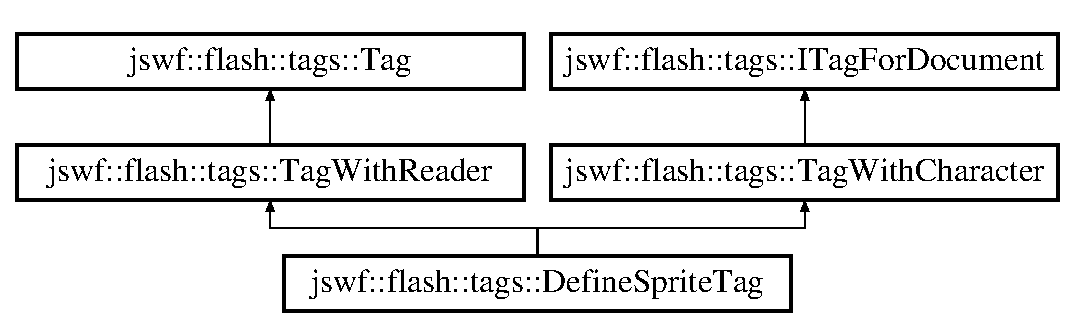
\includegraphics[height=3.000000cm]{classjswf_1_1flash_1_1tags_1_1_define_sprite_tag}
\end{center}
\end{figure}
\subsection*{Public Member Functions}
\begin{DoxyCompactItemize}
\item 
\hypertarget{classjswf_1_1flash_1_1tags_1_1_define_sprite_tag_a84381c81d866db76cf7a75b449a25580}{{\bfseries Define\+Sprite\+Tag} (tag\+\_\+type\+\_\+t t, std\+::string \&p)}\label{classjswf_1_1flash_1_1tags_1_1_define_sprite_tag_a84381c81d866db76cf7a75b449a25580}

\end{DoxyCompactItemize}
\subsection*{Public Attributes}
\begin{DoxyCompactItemize}
\item 
\hypertarget{classjswf_1_1flash_1_1tags_1_1_define_sprite_tag_a5154f9bde28145e313ae7fba40e0fd52}{\hyperlink{classjswf_1_1flash_1_1_sprite}{Sprite} $\ast$ {\bfseries sprite}}\label{classjswf_1_1flash_1_1tags_1_1_define_sprite_tag_a5154f9bde28145e313ae7fba40e0fd52}

\end{DoxyCompactItemize}


\subsection{Detailed Description}
Parses a {\ttfamily S\+P\+R\+I\+T\+E} record that is to be added to the document's {\ttfamily D\+I\+C\+T\+I\+O\+N\+A\+R\+Y}. 

The documentation for this class was generated from the following file\+:\begin{DoxyCompactItemize}
\item 
jswf/flash/tags/Define\+Sprite\+Tag.\+h\end{DoxyCompactItemize}

\hypertarget{classjswf_1_1avm2_1_1ast_1_1_definition_node}{\section{jswf\+:\+:avm2\+:\+:ast\+:\+:Definition\+Node Class Reference}
\label{classjswf_1_1avm2_1_1ast_1_1_definition_node}\index{jswf\+::avm2\+::ast\+::\+Definition\+Node@{jswf\+::avm2\+::ast\+::\+Definition\+Node}}
}


Describes a declaration of a local variable.  




{\ttfamily \#include $<$Node.\+h$>$}

Inheritance diagram for jswf\+:\+:avm2\+:\+:ast\+:\+:Definition\+Node\+:\begin{figure}[H]
\begin{center}
\leavevmode
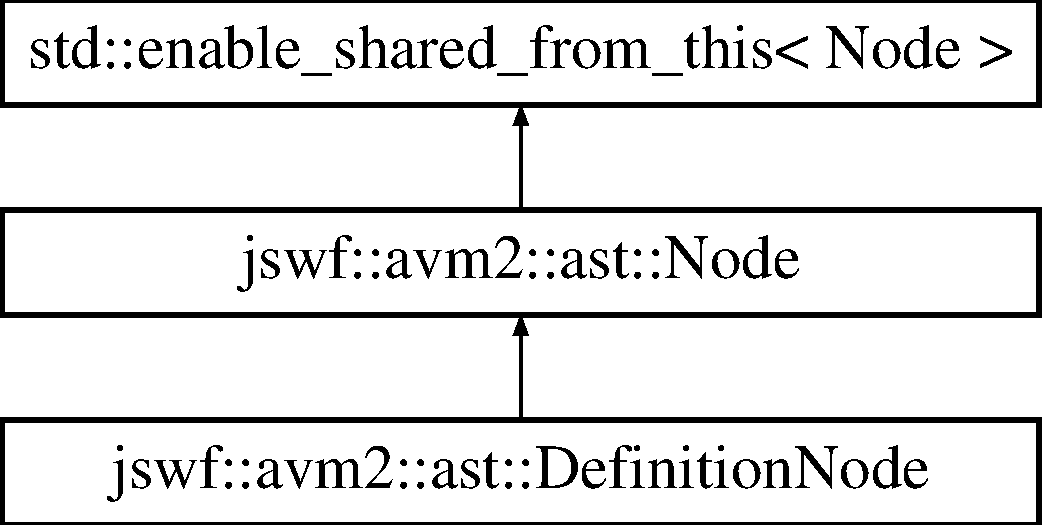
\includegraphics[height=3.000000cm]{classjswf_1_1avm2_1_1ast_1_1_definition_node}
\end{center}
\end{figure}
\subsection*{Public Member Functions}
\begin{DoxyCompactItemize}
\item 
\hypertarget{classjswf_1_1avm2_1_1ast_1_1_definition_node_a5c64f80e2ae2503f7f69feac7439d646}{{\bfseries Definition\+Node} (Node\+Ptr n)}\label{classjswf_1_1avm2_1_1ast_1_1_definition_node_a5c64f80e2ae2503f7f69feac7439d646}

\item 
\hypertarget{classjswf_1_1avm2_1_1ast_1_1_definition_node_a07f6fa62d6bed6a2f7eda2b593dc6644}{virtual std\+::string {\bfseries to\+String} ()}\label{classjswf_1_1avm2_1_1ast_1_1_definition_node_a07f6fa62d6bed6a2f7eda2b593dc6644}

\end{DoxyCompactItemize}
\subsection*{Public Attributes}
\begin{DoxyCompactItemize}
\item 
\hypertarget{classjswf_1_1avm2_1_1ast_1_1_definition_node_a32afc61156fda02394fbec80fa9e779d}{Node\+Ptr {\bfseries local\+Node}}\label{classjswf_1_1avm2_1_1ast_1_1_definition_node_a32afc61156fda02394fbec80fa9e779d}

\end{DoxyCompactItemize}


\subsection{Detailed Description}
Describes a declaration of a local variable. 

\begin{DoxyRefDesc}{Todo}
\item[\hyperlink{todo__todo000006}{Todo}]This should be {\ttfamily Declaration\+Node} \end{DoxyRefDesc}


The documentation for this class was generated from the following file\+:\begin{DoxyCompactItemize}
\item 
jswf/avm2/ast/Node.\+h\end{DoxyCompactItemize}

\hypertarget{classjswf_1_1avm2_1_1ast_1_1_diadic_node}{\section{jswf\+:\+:avm2\+:\+:ast\+:\+:Diadic\+Node Class Reference}
\label{classjswf_1_1avm2_1_1ast_1_1_diadic_node}\index{jswf\+::avm2\+::ast\+::\+Diadic\+Node@{jswf\+::avm2\+::ast\+::\+Diadic\+Node}}
}


Describes a diadic operation.  




{\ttfamily \#include $<$Node.\+h$>$}

Inheritance diagram for jswf\+:\+:avm2\+:\+:ast\+:\+:Diadic\+Node\+:\begin{figure}[H]
\begin{center}
\leavevmode
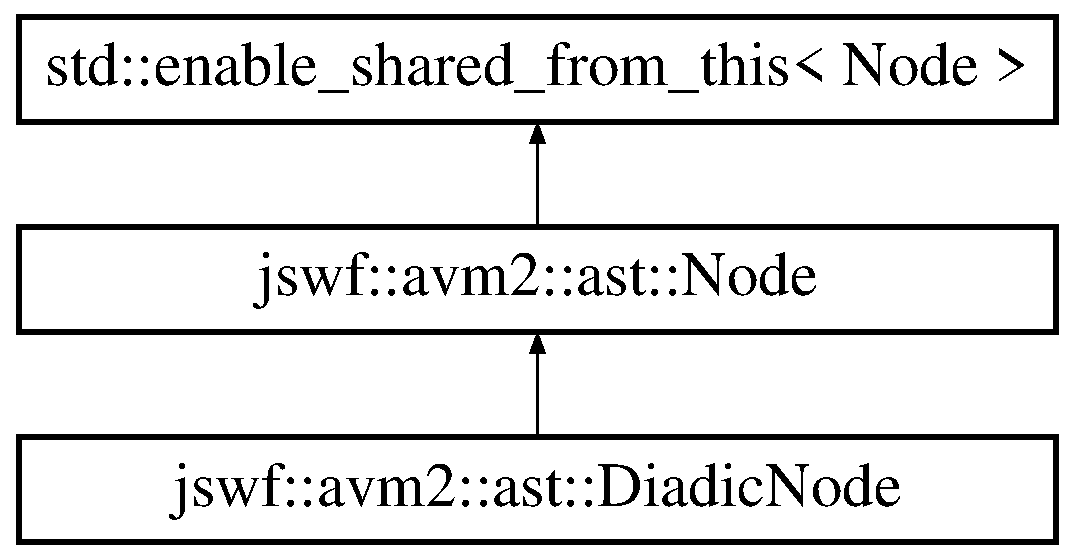
\includegraphics[height=3.000000cm]{classjswf_1_1avm2_1_1ast_1_1_diadic_node}
\end{center}
\end{figure}
\subsection*{Public Member Functions}
\begin{DoxyCompactItemize}
\item 
\hypertarget{classjswf_1_1avm2_1_1ast_1_1_diadic_node_a837163942ca9da3084897913fbc01b5d}{{\bfseries Diadic\+Node} (Node\+Ptr right, Node\+Ptr left, std\+::string op, int p)}\label{classjswf_1_1avm2_1_1ast_1_1_diadic_node_a837163942ca9da3084897913fbc01b5d}

\item 
\hypertarget{classjswf_1_1avm2_1_1ast_1_1_diadic_node_a2629df7becea46cb2ce5bad37d745b34}{virtual std\+::string {\bfseries to\+String} ()}\label{classjswf_1_1avm2_1_1ast_1_1_diadic_node_a2629df7becea46cb2ce5bad37d745b34}

\end{DoxyCompactItemize}
\subsection*{Public Attributes}
\begin{DoxyCompactItemize}
\item 
\hypertarget{classjswf_1_1avm2_1_1ast_1_1_diadic_node_a2c63a82d584784aa229b6b2675d0fbf3}{Node\+Ptr {\bfseries left}}\label{classjswf_1_1avm2_1_1ast_1_1_diadic_node_a2c63a82d584784aa229b6b2675d0fbf3}

\item 
\hypertarget{classjswf_1_1avm2_1_1ast_1_1_diadic_node_a5fecfc23e6424111988fb2c2f9c2b010}{Node\+Ptr {\bfseries right}}\label{classjswf_1_1avm2_1_1ast_1_1_diadic_node_a5fecfc23e6424111988fb2c2f9c2b010}

\item 
\hypertarget{classjswf_1_1avm2_1_1ast_1_1_diadic_node_a0b715d629e534f2d22e199e8fd98dfa3}{std\+::string {\bfseries op}}\label{classjswf_1_1avm2_1_1ast_1_1_diadic_node_a0b715d629e534f2d22e199e8fd98dfa3}

\end{DoxyCompactItemize}


\subsection{Detailed Description}
Describes a diadic operation. 

The documentation for this class was generated from the following file\+:\begin{DoxyCompactItemize}
\item 
jswf/avm2/ast/Node.\+h\end{DoxyCompactItemize}

\hypertarget{structjswf_1_1flash_1_1_display_list_entry}{\section{jswf\+:\+:flash\+:\+:Display\+List\+Entry Struct Reference}
\label{structjswf_1_1flash_1_1_display_list_entry}\index{jswf\+::flash\+::\+Display\+List\+Entry@{jswf\+::flash\+::\+Display\+List\+Entry}}
}


{\ttfamily \#include $<$Frame.\+h$>$}

\subsection*{Public Attributes}
\begin{DoxyCompactItemize}
\item 
\hypertarget{structjswf_1_1flash_1_1_display_list_entry_a8bae9b8a903b5dba94f5b6f82444ddb3}{uint16\+\_\+t {\bfseries character\+Id}}\label{structjswf_1_1flash_1_1_display_list_entry_a8bae9b8a903b5dba94f5b6f82444ddb3}

\item 
\hypertarget{structjswf_1_1flash_1_1_display_list_entry_a0ccf4f431308416dd030b69197865bfc}{avm2\+::\+Object\+Ptr {\bfseries avm2\+Object} = N\+U\+L\+L}\label{structjswf_1_1flash_1_1_display_list_entry_a0ccf4f431308416dd030b69197865bfc}

\item 
\hypertarget{structjswf_1_1flash_1_1_display_list_entry_a5b1eba4da61f771da0f058ec580ed5e6}{avm2\+::\+Object\+Ptr {\bfseries on\+Enter\+Frame} = N\+U\+L\+L}\label{structjswf_1_1flash_1_1_display_list_entry_a5b1eba4da61f771da0f058ec580ed5e6}

\item 
\hypertarget{structjswf_1_1flash_1_1_display_list_entry_af91ac80206f164a044f705737815f869}{bool \hyperlink{structjswf_1_1flash_1_1_display_list_entry_af91ac80206f164a044f705737815f869}{use\+Previous\+Matrix} = false}\label{structjswf_1_1flash_1_1_display_list_entry_af91ac80206f164a044f705737815f869}

\begin{DoxyCompactList}\small\item\em Set to {\ttfamily true} if matrix was altered by a script and has to be kept. \end{DoxyCompactList}\item 
\hypertarget{structjswf_1_1flash_1_1_display_list_entry_a32fdfad6013761553087b7cd94a2e208}{bool {\bfseries does\+Clip} = false}\label{structjswf_1_1flash_1_1_display_list_entry_a32fdfad6013761553087b7cd94a2e208}

\item 
\hypertarget{structjswf_1_1flash_1_1_display_list_entry_ae5eb13f0f96f4313c60f181d52fb329e}{uint16\+\_\+t {\bfseries clip\+Depth}}\label{structjswf_1_1flash_1_1_display_list_entry_ae5eb13f0f96f4313c60f181d52fb329e}

\item 
\hypertarget{structjswf_1_1flash_1_1_display_list_entry_a34005f670c4b2a3608ad54a084d71b3a}{bool {\bfseries sets\+Color\+Transform} = false}\label{structjswf_1_1flash_1_1_display_list_entry_a34005f670c4b2a3608ad54a084d71b3a}

\item 
\hypertarget{structjswf_1_1flash_1_1_display_list_entry_aafb3c754661465d530a59ed09334bc04}{\hyperlink{structjswf_1_1flash_1_1_matrix}{Matrix} {\bfseries matrix}}\label{structjswf_1_1flash_1_1_display_list_entry_aafb3c754661465d530a59ed09334bc04}

\item 
\hypertarget{structjswf_1_1flash_1_1_display_list_entry_a868636e7c8d50e8d556c6b75a3fbae9d}{\hyperlink{structjswf_1_1flash_1_1_color_transform}{Color\+Transform} {\bfseries color\+Transform}}\label{structjswf_1_1flash_1_1_display_list_entry_a868636e7c8d50e8d556c6b75a3fbae9d}

\end{DoxyCompactItemize}


\subsection{Detailed Description}
\begin{DoxyRefDesc}{Todo}
\item[\hyperlink{todo__todo000011}{Todo}]Should structures implement read/write themselves? 

This structure is wrong. {\ttfamily use\+Previous\+Matrix} can be replaced with a {\ttfamily get\+Property}-\/test on our {\ttfamily avm2\+Object} with a fallback to {\ttfamily matrix}. Also, {\ttfamily avm2\+Object} will not properly work in nested environments (tree structures). Same thing with modifications by A\+V\+M2 (adding/removing Display\+Objects). \end{DoxyRefDesc}


The documentation for this struct was generated from the following file\+:\begin{DoxyCompactItemize}
\item 
jswf/flash/Frame.\+h\end{DoxyCompactItemize}

\hypertarget{classjswf_1_1avm2_1_1_display_object}{\section{jswf\+:\+:avm2\+:\+:Display\+Object Class Reference}
\label{classjswf_1_1avm2_1_1_display_object}\index{jswf\+::avm2\+::\+Display\+Object@{jswf\+::avm2\+::\+Display\+Object}}
}
Inheritance diagram for jswf\+:\+:avm2\+:\+:Display\+Object\+:\begin{figure}[H]
\begin{center}
\leavevmode
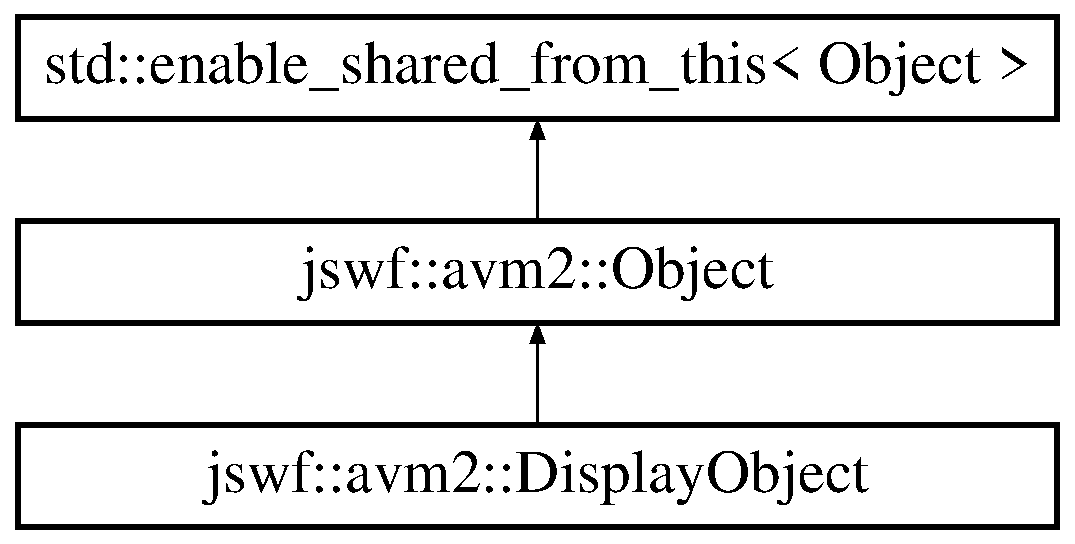
\includegraphics[height=3.000000cm]{classjswf_1_1avm2_1_1_display_object}
\end{center}
\end{figure}
\subsection*{Public Member Functions}
\begin{DoxyCompactItemize}
\item 
\hypertarget{classjswf_1_1avm2_1_1_display_object_a21dbe0d8901758a89fe6281733d78d3f}{{\bfseries Display\+Object} (\hyperlink{classjswf_1_1avm2_1_1_v_m}{V\+M} $\ast$vm, \hyperlink{classjswf_1_1avm2_1_1_class}{Class} $\ast$klass, \hyperlink{structjswf_1_1flash_1_1_display_list_entry}{flash\+::\+Display\+List\+Entry} $\ast$value)}\label{classjswf_1_1avm2_1_1_display_object_a21dbe0d8901758a89fe6281733d78d3f}

\item 
\hypertarget{classjswf_1_1avm2_1_1_display_object_afe14733203066e32329bb2441c1327b3}{void {\bfseries set\+Property} (const \hyperlink{structjswf_1_1avm2_1_1_multiname}{Multiname} \&property, const Object\+Ptr \&value)}\label{classjswf_1_1avm2_1_1_display_object_afe14733203066e32329bb2441c1327b3}

\end{DoxyCompactItemize}
\subsection*{Public Attributes}
\begin{DoxyCompactItemize}
\item 
\hypertarget{classjswf_1_1avm2_1_1_display_object_a8786424f1b28392cdef1ed13b97d9493}{double {\bfseries rotation} = 1}\label{classjswf_1_1avm2_1_1_display_object_a8786424f1b28392cdef1ed13b97d9493}

\item 
\hypertarget{classjswf_1_1avm2_1_1_display_object_ad124b9b28b42663f930a774dd84ce7b8}{double {\bfseries scale\+X} = 1}\label{classjswf_1_1avm2_1_1_display_object_ad124b9b28b42663f930a774dd84ce7b8}

\item 
\hypertarget{classjswf_1_1avm2_1_1_display_object_a6f0c828bb8025f81a81f878687272b44}{double {\bfseries scale\+Y} = 1}\label{classjswf_1_1avm2_1_1_display_object_a6f0c828bb8025f81a81f878687272b44}

\item 
\hypertarget{classjswf_1_1avm2_1_1_display_object_a7b52b41f451ff9950140e25e4f7343a3}{\hyperlink{structjswf_1_1flash_1_1_display_list_entry}{flash\+::\+Display\+List\+Entry} $\ast$ {\bfseries value}}\label{classjswf_1_1avm2_1_1_display_object_a7b52b41f451ff9950140e25e4f7343a3}

\end{DoxyCompactItemize}
\subsection*{Additional Inherited Members}


The documentation for this class was generated from the following files\+:\begin{DoxyCompactItemize}
\item 
jswf/avm2/Object.\+h\item 
jswf/avm2/Object.\+cpp\end{DoxyCompactItemize}

\hypertarget{classjswf_1_1flash_1_1tags_1_1_do_a_b_c_tag}{\section{jswf\+:\+:flash\+:\+:tags\+:\+:Do\+A\+B\+C\+Tag Class Reference}
\label{classjswf_1_1flash_1_1tags_1_1_do_a_b_c_tag}\index{jswf\+::flash\+::tags\+::\+Do\+A\+B\+C\+Tag@{jswf\+::flash\+::tags\+::\+Do\+A\+B\+C\+Tag}}
}


Carries an {\ttfamily \hyperlink{classjswf_1_1avm2_1_1_a_b_c_file}{avm2\+::\+A\+B\+C\+File}} to be executed by the \hyperlink{classjswf_1_1avm2_1_1_v_m}{avm2\+::\+V\+M}.  




{\ttfamily \#include $<$Do\+A\+B\+C\+Tag.\+h$>$}

Inheritance diagram for jswf\+:\+:flash\+:\+:tags\+:\+:Do\+A\+B\+C\+Tag\+:\begin{figure}[H]
\begin{center}
\leavevmode
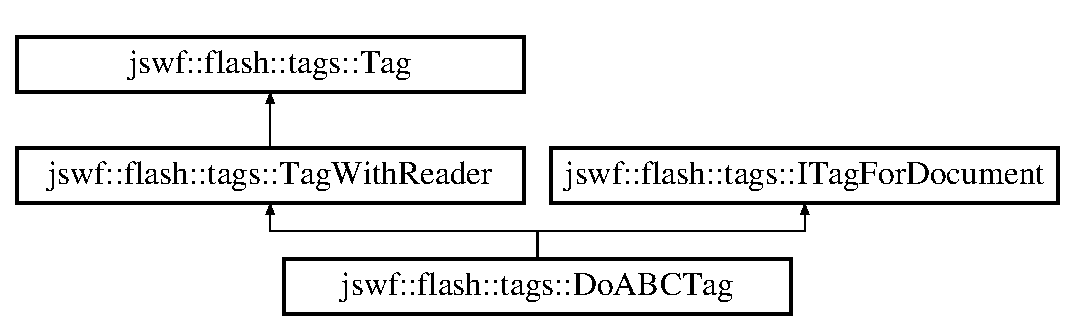
\includegraphics[height=3.000000cm]{classjswf_1_1flash_1_1tags_1_1_do_a_b_c_tag}
\end{center}
\end{figure}
\subsection*{Public Member Functions}
\begin{DoxyCompactItemize}
\item 
\hypertarget{classjswf_1_1flash_1_1tags_1_1_do_a_b_c_tag_aa6535b97433481386663fcc15de1facd}{{\bfseries Do\+A\+B\+C\+Tag} (tag\+\_\+type\+\_\+t t, std\+::string \&p)}\label{classjswf_1_1flash_1_1tags_1_1_do_a_b_c_tag_aa6535b97433481386663fcc15de1facd}

\item 
\hypertarget{classjswf_1_1flash_1_1tags_1_1_do_a_b_c_tag_a7ca7c629347fdfbab3d39bed07f79d76}{void {\bfseries apply\+To\+Document} (\hyperlink{classjswf_1_1flash_1_1_document}{Document} \&document)}\label{classjswf_1_1flash_1_1tags_1_1_do_a_b_c_tag_a7ca7c629347fdfbab3d39bed07f79d76}

\end{DoxyCompactItemize}
\subsection*{Public Attributes}
\begin{DoxyCompactItemize}
\item 
\hypertarget{classjswf_1_1flash_1_1tags_1_1_do_a_b_c_tag_a092de318a6947b04ab94dfd663a33e72}{uint32\+\_\+t {\bfseries flags}}\label{classjswf_1_1flash_1_1tags_1_1_do_a_b_c_tag_a092de318a6947b04ab94dfd663a33e72}

\item 
\hypertarget{classjswf_1_1flash_1_1tags_1_1_do_a_b_c_tag_ab890fd63f6ae2d3f9cd2138d85bf3c87}{std\+::string {\bfseries name}}\label{classjswf_1_1flash_1_1tags_1_1_do_a_b_c_tag_ab890fd63f6ae2d3f9cd2138d85bf3c87}

\item 
\hypertarget{classjswf_1_1flash_1_1tags_1_1_do_a_b_c_tag_ac21ee7ac4ac727b73faadd9f4cbc8be6}{std\+::shared\+\_\+ptr$<$ \hyperlink{classjswf_1_1avm2_1_1_a_b_c_file}{avm2\+::\+A\+B\+C\+File} $>$ {\bfseries abc}}\label{classjswf_1_1flash_1_1tags_1_1_do_a_b_c_tag_ac21ee7ac4ac727b73faadd9f4cbc8be6}

\end{DoxyCompactItemize}


\subsection{Detailed Description}
Carries an {\ttfamily \hyperlink{classjswf_1_1avm2_1_1_a_b_c_file}{avm2\+::\+A\+B\+C\+File}} to be executed by the \hyperlink{classjswf_1_1avm2_1_1_v_m}{avm2\+::\+V\+M}. 

The documentation for this class was generated from the following file\+:\begin{DoxyCompactItemize}
\item 
jswf/flash/tags/Do\+A\+B\+C\+Tag.\+h\end{DoxyCompactItemize}

\hypertarget{classjswf_1_1flash_1_1_document}{\section{jswf\+:\+:flash\+:\+:Document Class Reference}
\label{classjswf_1_1flash_1_1_document}\index{jswf\+::flash\+::\+Document@{jswf\+::flash\+::\+Document}}
}


Parses and represents a {\ttfamily S\+W\+F file}.  




{\ttfamily \#include $<$Document.\+h$>$}

\subsection*{Public Member Functions}
\begin{DoxyCompactItemize}
\item 
\hypertarget{classjswf_1_1flash_1_1_document_ab5cf654ae338ce454f48e5c972bad5e7}{{\bfseries Document} (std\+::shared\+\_\+ptr$<$ \hyperlink{classjswf_1_1io_1_1_generic_reader}{jswf\+::io\+::\+Generic\+Reader} $>$ \hyperlink{classjswf_1_1flash_1_1_document_abc03a4a547e56b1117423589edad89e4}{reader})}\label{classjswf_1_1flash_1_1_document_ab5cf654ae338ce454f48e5c972bad5e7}

\end{DoxyCompactItemize}
\subsection*{Public Attributes}
\begin{DoxyCompactItemize}
\item 
\hypertarget{classjswf_1_1flash_1_1_document_ad72642b03597be4ad76a41d524d05913}{\hyperlink{structjswf_1_1flash_1_1_header}{Header} \hyperlink{classjswf_1_1flash_1_1_document_ad72642b03597be4ad76a41d524d05913}{header}}\label{classjswf_1_1flash_1_1_document_ad72642b03597be4ad76a41d524d05913}

\begin{DoxyCompactList}\small\item\em The {\ttfamily H\+E\+A\+D\+E\+R} record for this document. \end{DoxyCompactList}\item 
\hypertarget{classjswf_1_1flash_1_1_document_adaacad383fad582fe94a14c44782123f}{\hyperlink{classjswf_1_1avm2_1_1_v_m}{avm2\+::\+V\+M} {\bfseries avm2}}\label{classjswf_1_1flash_1_1_document_adaacad383fad582fe94a14c44782123f}

\item 
\hypertarget{classjswf_1_1flash_1_1_document_ac2c8471be7e7cde4660b4183c0f29bba}{std\+::vector$<$ std\+::shared\+\_\+ptr\\*
$<$ \hyperlink{classjswf_1_1flash_1_1tags_1_1_tag}{tags\+::\+Tag} $>$ $>$ \hyperlink{classjswf_1_1flash_1_1_document_ac2c8471be7e7cde4660b4183c0f29bba}{tags}}\label{classjswf_1_1flash_1_1_document_ac2c8471be7e7cde4660b4183c0f29bba}

\begin{DoxyCompactList}\small\item\em A {\ttfamily vector} of {\ttfamily shared\+\_\+ptr}s to the tags this document contains. \end{DoxyCompactList}\item 
\hypertarget{classjswf_1_1flash_1_1_document_aca1e9bbd368ff49f61d59a4fed7754a9}{std\+::map$<$ uint16\+\_\+t, \\*
std\+::shared\+\_\+ptr$<$ \hyperlink{classjswf_1_1flash_1_1_character}{Character} $>$ $>$ \hyperlink{classjswf_1_1flash_1_1_document_aca1e9bbd368ff49f61d59a4fed7754a9}{dictionary}}\label{classjswf_1_1flash_1_1_document_aca1e9bbd368ff49f61d59a4fed7754a9}

\begin{DoxyCompactList}\small\item\em The {\ttfamily D\+I\+C\+T\+I\+O\+N\+A\+R\+Y} of this document. \end{DoxyCompactList}\item 
\hyperlink{classjswf_1_1flash_1_1_sprite}{Sprite} $\ast$ \hyperlink{classjswf_1_1flash_1_1_document_a2b85a878280ace8647cb05fdfd79e22a}{root\+Sprite}
\end{DoxyCompactItemize}
\subsection*{Protected Attributes}
\begin{DoxyCompactItemize}
\item 
\hypertarget{classjswf_1_1flash_1_1_document_abc03a4a547e56b1117423589edad89e4}{\hyperlink{classjswf_1_1flash_1_1_reader}{Reader} \hyperlink{classjswf_1_1flash_1_1_document_abc03a4a547e56b1117423589edad89e4}{reader}}\label{classjswf_1_1flash_1_1_document_abc03a4a547e56b1117423589edad89e4}

\begin{DoxyCompactList}\small\item\em The \hyperlink{classjswf_1_1flash_1_1_reader}{flash\+::\+Reader} used by this document. \end{DoxyCompactList}\end{DoxyCompactItemize}


\subsection{Detailed Description}
Parses and represents a {\ttfamily S\+W\+F file}. 

\begin{DoxyRefDesc}{Todo}
\item[\hyperlink{todo__todo000009}{Todo}]\hyperlink{classjswf_1_1flash_1_1_document_ac2c8471be7e7cde4660b4183c0f29bba}{Document\+::tags} and Sprite\+::tags ? Somewhat redundant. \begin{DoxySeeAlso}{See also}
I\+Tag\+For\+Document 
\end{DoxySeeAlso}
\end{DoxyRefDesc}


\subsection{Member Data Documentation}
\hypertarget{classjswf_1_1flash_1_1_document_a2b85a878280ace8647cb05fdfd79e22a}{\index{jswf\+::flash\+::\+Document@{jswf\+::flash\+::\+Document}!root\+Sprite@{root\+Sprite}}
\index{root\+Sprite@{root\+Sprite}!jswf\+::flash\+::\+Document@{jswf\+::flash\+::\+Document}}
\subsubsection[{root\+Sprite}]{\setlength{\rightskip}{0pt plus 5cm}{\bf Sprite}$\ast$ jswf\+::flash\+::\+Document\+::root\+Sprite}}\label{classjswf_1_1flash_1_1_document_a2b85a878280ace8647cb05fdfd79e22a}
\begin{DoxyRefDesc}{Todo}
\item[\hyperlink{todo__todo000010}{Todo}]This is the main\+\_\+timeline object! It can also be transformed! \end{DoxyRefDesc}


The documentation for this class was generated from the following files\+:\begin{DoxyCompactItemize}
\item 
jswf/flash/Document.\+h\item 
jswf/flash/Document.\+cpp\end{DoxyCompactItemize}

\hypertarget{classjswf_1_1avm2_1_1ast_1_1_double_node}{\section{jswf\+:\+:avm2\+:\+:ast\+:\+:Double\+Node Class Reference}
\label{classjswf_1_1avm2_1_1ast_1_1_double_node}\index{jswf\+::avm2\+::ast\+::\+Double\+Node@{jswf\+::avm2\+::ast\+::\+Double\+Node}}
}


Describes a node that carries a double literal.  




{\ttfamily \#include $<$Node.\+h$>$}

Inheritance diagram for jswf\+:\+:avm2\+:\+:ast\+:\+:Double\+Node\+:\begin{figure}[H]
\begin{center}
\leavevmode
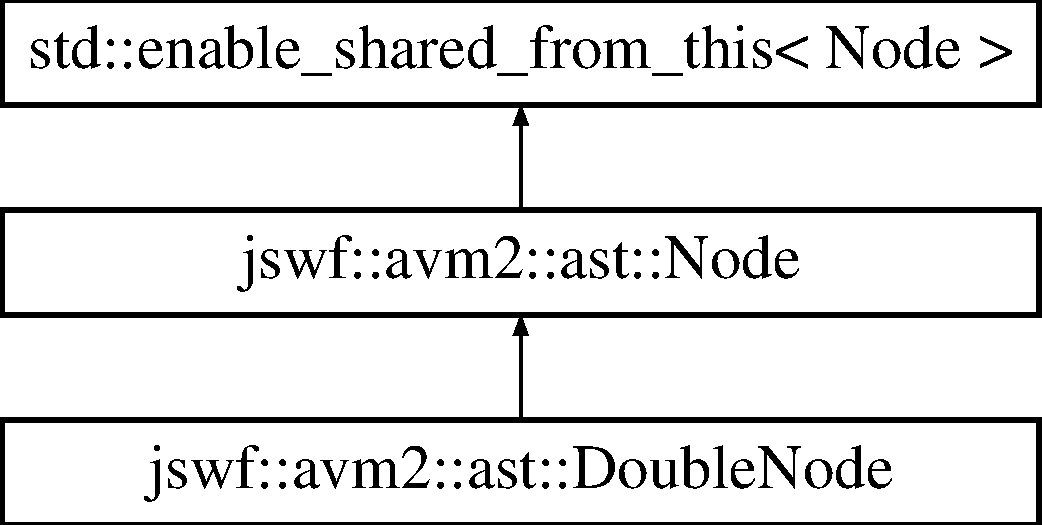
\includegraphics[height=3.000000cm]{classjswf_1_1avm2_1_1ast_1_1_double_node}
\end{center}
\end{figure}
\subsection*{Public Member Functions}
\begin{DoxyCompactItemize}
\item 
\hypertarget{classjswf_1_1avm2_1_1ast_1_1_double_node_a2c8d42f7d6e53b861d1d06ba37346fd4}{{\bfseries Double\+Node} (double dbl)}\label{classjswf_1_1avm2_1_1ast_1_1_double_node_a2c8d42f7d6e53b861d1d06ba37346fd4}

\item 
\hypertarget{classjswf_1_1avm2_1_1ast_1_1_double_node_afd147c85f01bc0ee9c273b996669bb88}{virtual std\+::string {\bfseries to\+String} ()}\label{classjswf_1_1avm2_1_1ast_1_1_double_node_afd147c85f01bc0ee9c273b996669bb88}

\end{DoxyCompactItemize}
\subsection*{Public Attributes}
\begin{DoxyCompactItemize}
\item 
\hypertarget{classjswf_1_1avm2_1_1ast_1_1_double_node_a7800c126b9a9d8e7e4f7f3a4653a7682}{double {\bfseries value}}\label{classjswf_1_1avm2_1_1ast_1_1_double_node_a7800c126b9a9d8e7e4f7f3a4653a7682}

\end{DoxyCompactItemize}


\subsection{Detailed Description}
Describes a node that carries a double literal. 

The documentation for this class was generated from the following file\+:\begin{DoxyCompactItemize}
\item 
jswf/avm2/ast/Node.\+h\end{DoxyCompactItemize}

\hypertarget{structjswf_1_1avm2_1_1_e_c_m_a_hint}{\section{jswf\+:\+:avm2\+:\+:E\+C\+M\+A\+Hint Struct Reference}
\label{structjswf_1_1avm2_1_1_e_c_m_a_hint}\index{jswf\+::avm2\+::\+E\+C\+M\+A\+Hint@{jswf\+::avm2\+::\+E\+C\+M\+A\+Hint}}
}
\subsection*{Public Types}
\begin{DoxyCompactItemize}
\item 
\hypertarget{structjswf_1_1avm2_1_1_e_c_m_a_hint_a7f858509585153bc8e03cd355edaf22f}{enum {\bfseries Enum} \{ {\bfseries No\+Hint} = 0, 
{\bfseries Number\+Hint}, 
{\bfseries String\+Hint}
 \}}\label{structjswf_1_1avm2_1_1_e_c_m_a_hint_a7f858509585153bc8e03cd355edaf22f}

\end{DoxyCompactItemize}


The documentation for this struct was generated from the following file\+:\begin{DoxyCompactItemize}
\item 
jswf/avm2/Object.\+h\end{DoxyCompactItemize}

\hypertarget{structjswf_1_1flash_1_1_edge}{\section{jswf\+:\+:flash\+:\+:Edge Struct Reference}
\label{structjswf_1_1flash_1_1_edge}\index{jswf\+::flash\+::\+Edge@{jswf\+::flash\+::\+Edge}}
}


Represents an edge between two instances of \hyperlink{structjswf_1_1flash_1_1_point}{Point}.  




{\ttfamily \#include $<$Shape.\+h$>$}

\subsection*{Public Attributes}
\begin{DoxyCompactItemize}
\item 
\hypertarget{structjswf_1_1flash_1_1_edge_a9342bb598582a1662085a2216b22e79d}{\hyperlink{structjswf_1_1flash_1_1_point}{Point} \hyperlink{structjswf_1_1flash_1_1_edge_a9342bb598582a1662085a2216b22e79d}{a}}\label{structjswf_1_1flash_1_1_edge_a9342bb598582a1662085a2216b22e79d}

\begin{DoxyCompactList}\small\item\em Starting point of the edge. \end{DoxyCompactList}\item 
\hypertarget{structjswf_1_1flash_1_1_edge_a14859e594a6bb8a7bee90cc200080f7c}{\hyperlink{structjswf_1_1flash_1_1_point}{Point} \hyperlink{structjswf_1_1flash_1_1_edge_a14859e594a6bb8a7bee90cc200080f7c}{b}}\label{structjswf_1_1flash_1_1_edge_a14859e594a6bb8a7bee90cc200080f7c}

\begin{DoxyCompactList}\small\item\em End point of the edge. \end{DoxyCompactList}\end{DoxyCompactItemize}


\subsection{Detailed Description}
Represents an edge between two instances of \hyperlink{structjswf_1_1flash_1_1_point}{Point}. 

The documentation for this struct was generated from the following file\+:\begin{DoxyCompactItemize}
\item 
jswf/flash/Shape.\+h\end{DoxyCompactItemize}

\hypertarget{classjswf_1_1flash_1_1tags_1_1_end_tag}{\section{jswf\+:\+:flash\+:\+:tags\+:\+:End\+Tag Class Reference}
\label{classjswf_1_1flash_1_1tags_1_1_end_tag}\index{jswf\+::flash\+::tags\+::\+End\+Tag@{jswf\+::flash\+::tags\+::\+End\+Tag}}
}


Marks the end of a tag array and thereby the end of a \hyperlink{classjswf_1_1flash_1_1_document}{Document} or \hyperlink{classjswf_1_1flash_1_1_sprite}{Sprite}.  




{\ttfamily \#include $<$End\+Tag.\+h$>$}

Inheritance diagram for jswf\+:\+:flash\+:\+:tags\+:\+:End\+Tag\+:\begin{figure}[H]
\begin{center}
\leavevmode
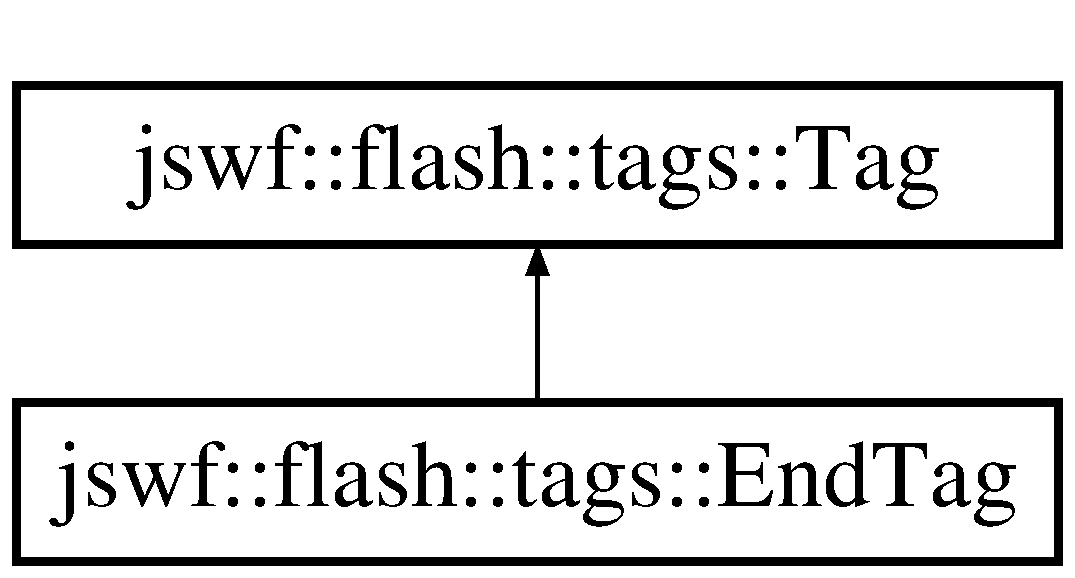
\includegraphics[height=2.000000cm]{classjswf_1_1flash_1_1tags_1_1_end_tag}
\end{center}
\end{figure}
\subsection*{Public Member Functions}
\begin{DoxyCompactItemize}
\item 
\hypertarget{classjswf_1_1flash_1_1tags_1_1_end_tag_a03e91c253ceeafebef3ec1f8c19780a4}{{\bfseries End\+Tag} (tag\+\_\+type\+\_\+t t, std\+::string \&p)}\label{classjswf_1_1flash_1_1tags_1_1_end_tag_a03e91c253ceeafebef3ec1f8c19780a4}

\end{DoxyCompactItemize}
\subsection*{Additional Inherited Members}


\subsection{Detailed Description}
Marks the end of a tag array and thereby the end of a \hyperlink{classjswf_1_1flash_1_1_document}{Document} or \hyperlink{classjswf_1_1flash_1_1_sprite}{Sprite}. 

\begin{DoxySeeAlso}{See also}
\hyperlink{classjswf_1_1flash_1_1_document}{flash\+::\+Document} 

\hyperlink{classjswf_1_1flash_1_1tags_1_1_define_sprite_tag}{flash\+::tags\+::\+Define\+Sprite\+Tag} 
\end{DoxySeeAlso}


The documentation for this class was generated from the following file\+:\begin{DoxyCompactItemize}
\item 
jswf/flash/tags/End\+Tag.\+h\end{DoxyCompactItemize}

\hypertarget{structjswf_1_1avm2_1_1_exception_info}{\section{jswf\+:\+:avm2\+:\+:Exception\+Info Struct Reference}
\label{structjswf_1_1avm2_1_1_exception_info}\index{jswf\+::avm2\+::\+Exception\+Info@{jswf\+::avm2\+::\+Exception\+Info}}
}
\subsection*{Public Attributes}
\begin{DoxyCompactItemize}
\item 
\hypertarget{structjswf_1_1avm2_1_1_exception_info_a4ef6047a684a72cc1401449bec2a9562}{\hyperlink{namespacejswf_aa10d9ddca2a6a5debdc261dfae3d1117}{u30\+\_\+t} {\bfseries from}}\label{structjswf_1_1avm2_1_1_exception_info_a4ef6047a684a72cc1401449bec2a9562}

\item 
\hypertarget{structjswf_1_1avm2_1_1_exception_info_ac75072705ac36ad1756d76711df5f85d}{\hyperlink{namespacejswf_aa10d9ddca2a6a5debdc261dfae3d1117}{u30\+\_\+t} {\bfseries to}}\label{structjswf_1_1avm2_1_1_exception_info_ac75072705ac36ad1756d76711df5f85d}

\item 
\hypertarget{structjswf_1_1avm2_1_1_exception_info_ad406c052645131d062ba8361f64f8b31}{\hyperlink{namespacejswf_aa10d9ddca2a6a5debdc261dfae3d1117}{u30\+\_\+t} {\bfseries target}}\label{structjswf_1_1avm2_1_1_exception_info_ad406c052645131d062ba8361f64f8b31}

\item 
\hypertarget{structjswf_1_1avm2_1_1_exception_info_aeca3c60721a72c2d4bd7405dd105edd1}{\hyperlink{namespacejswf_aa10d9ddca2a6a5debdc261dfae3d1117}{u30\+\_\+t} {\bfseries exc\+Type}}\label{structjswf_1_1avm2_1_1_exception_info_aeca3c60721a72c2d4bd7405dd105edd1}

\item 
\hypertarget{structjswf_1_1avm2_1_1_exception_info_a1e01c3337cb192b9901fb64223b3f215}{\hyperlink{namespacejswf_aa10d9ddca2a6a5debdc261dfae3d1117}{u30\+\_\+t} {\bfseries var\+Name}}\label{structjswf_1_1avm2_1_1_exception_info_a1e01c3337cb192b9901fb64223b3f215}

\end{DoxyCompactItemize}


The documentation for this struct was generated from the following file\+:\begin{DoxyCompactItemize}
\item 
jswf/avm2/Method\+Info.\+h\end{DoxyCompactItemize}

\hypertarget{classjswf_1_1flash_1_1tags_1_1_file_attributes_tag}{\section{jswf\+:\+:flash\+:\+:tags\+:\+:File\+Attributes\+Tag Class Reference}
\label{classjswf_1_1flash_1_1tags_1_1_file_attributes_tag}\index{jswf\+::flash\+::tags\+::\+File\+Attributes\+Tag@{jswf\+::flash\+::tags\+::\+File\+Attributes\+Tag}}
}


Represents {\ttfamily File\+Attribute} tags.  




{\ttfamily \#include $<$File\+Attributes\+Tag.\+h$>$}

Inheritance diagram for jswf\+:\+:flash\+:\+:tags\+:\+:File\+Attributes\+Tag\+:\begin{figure}[H]
\begin{center}
\leavevmode
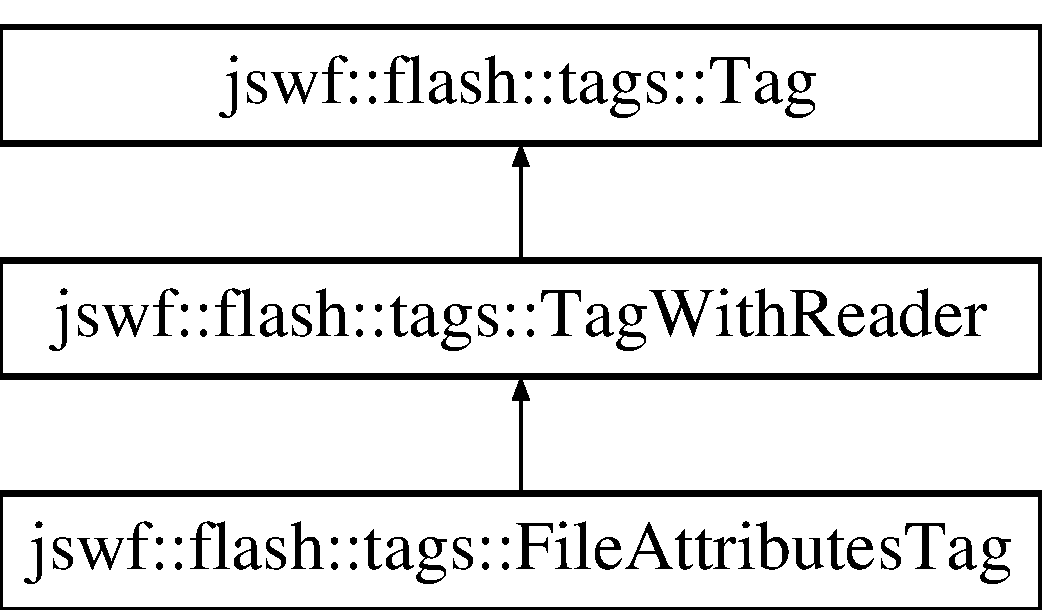
\includegraphics[height=3.000000cm]{classjswf_1_1flash_1_1tags_1_1_file_attributes_tag}
\end{center}
\end{figure}
\subsection*{Public Member Functions}
\begin{DoxyCompactItemize}
\item 
\hypertarget{classjswf_1_1flash_1_1tags_1_1_file_attributes_tag_a467831c52a097d2ed1dbd1dbf723624a}{{\bfseries File\+Attributes\+Tag} (tag\+\_\+type\+\_\+t t, std\+::string \&p)}\label{classjswf_1_1flash_1_1tags_1_1_file_attributes_tag_a467831c52a097d2ed1dbd1dbf723624a}

\end{DoxyCompactItemize}
\subsection*{Public Attributes}
\begin{DoxyCompactItemize}
\item 
\hypertarget{classjswf_1_1flash_1_1tags_1_1_file_attributes_tag_aa8b22f78f188684d9595d81db2fcfa0e}{bool {\bfseries use\+\_\+direct\+\_\+blit}}\label{classjswf_1_1flash_1_1tags_1_1_file_attributes_tag_aa8b22f78f188684d9595d81db2fcfa0e}

\item 
\hypertarget{classjswf_1_1flash_1_1tags_1_1_file_attributes_tag_aaadbf26d1d9c16e62048be7412839995}{bool {\bfseries use\+\_\+gpu}}\label{classjswf_1_1flash_1_1tags_1_1_file_attributes_tag_aaadbf26d1d9c16e62048be7412839995}

\item 
\hypertarget{classjswf_1_1flash_1_1tags_1_1_file_attributes_tag_afef5a090ce260e125c3b8c309928a11b}{bool {\bfseries has\+\_\+metadata}}\label{classjswf_1_1flash_1_1tags_1_1_file_attributes_tag_afef5a090ce260e125c3b8c309928a11b}

\item 
\hypertarget{classjswf_1_1flash_1_1tags_1_1_file_attributes_tag_acb853599995dec39a858e1905589662d}{bool {\bfseries is\+\_\+as3}}\label{classjswf_1_1flash_1_1tags_1_1_file_attributes_tag_acb853599995dec39a858e1905589662d}

\item 
\hypertarget{classjswf_1_1flash_1_1tags_1_1_file_attributes_tag_a6590aafd6d48cfae7693e4ff0ee06027}{bool {\bfseries use\+\_\+network}}\label{classjswf_1_1flash_1_1tags_1_1_file_attributes_tag_a6590aafd6d48cfae7693e4ff0ee06027}

\end{DoxyCompactItemize}


\subsection{Detailed Description}
Represents {\ttfamily File\+Attribute} tags. 

The documentation for this class was generated from the following file\+:\begin{DoxyCompactItemize}
\item 
jswf/flash/tags/File\+Attributes\+Tag.\+h\end{DoxyCompactItemize}

\hypertarget{classjswf_1_1flash_1_1styles_1_1_fill_style}{\section{jswf\+:\+:flash\+:\+:styles\+:\+:Fill\+Style Class Reference}
\label{classjswf_1_1flash_1_1styles_1_1_fill_style}\index{jswf\+::flash\+::styles\+::\+Fill\+Style@{jswf\+::flash\+::styles\+::\+Fill\+Style}}
}
Inheritance diagram for jswf\+:\+:flash\+:\+:styles\+:\+:Fill\+Style\+:\begin{figure}[H]
\begin{center}
\leavevmode
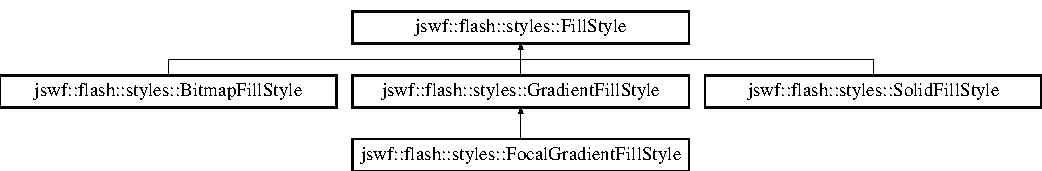
\includegraphics[height=2.295082cm]{classjswf_1_1flash_1_1styles_1_1_fill_style}
\end{center}
\end{figure}
\subsection*{Public Attributes}
\begin{DoxyCompactItemize}
\item 
\hypertarget{classjswf_1_1flash_1_1styles_1_1_fill_style_a68e25e6e215713f1b0b20da0d8b3be8b}{uint32\+\_\+t {\bfseries id}}\label{classjswf_1_1flash_1_1styles_1_1_fill_style_a68e25e6e215713f1b0b20da0d8b3be8b}

\end{DoxyCompactItemize}


The documentation for this class was generated from the following file\+:\begin{DoxyCompactItemize}
\item 
jswf/flash/styles/Fill\+Style.\+h\end{DoxyCompactItemize}

\hypertarget{classjswf_1_1flash_1_1styles_1_1_focal_gradient_fill_style}{\section{jswf\+:\+:flash\+:\+:styles\+:\+:Focal\+Gradient\+Fill\+Style Class Reference}
\label{classjswf_1_1flash_1_1styles_1_1_focal_gradient_fill_style}\index{jswf\+::flash\+::styles\+::\+Focal\+Gradient\+Fill\+Style@{jswf\+::flash\+::styles\+::\+Focal\+Gradient\+Fill\+Style}}
}
Inheritance diagram for jswf\+:\+:flash\+:\+:styles\+:\+:Focal\+Gradient\+Fill\+Style\+:\begin{figure}[H]
\begin{center}
\leavevmode
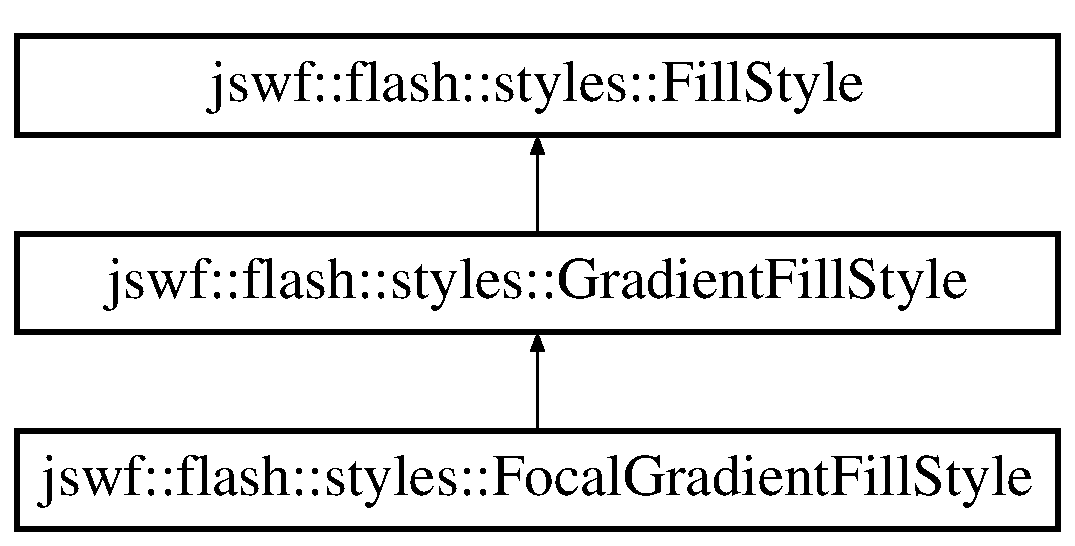
\includegraphics[height=3.000000cm]{classjswf_1_1flash_1_1styles_1_1_focal_gradient_fill_style}
\end{center}
\end{figure}
\subsection*{Public Attributes}
\begin{DoxyCompactItemize}
\item 
\hypertarget{classjswf_1_1flash_1_1styles_1_1_focal_gradient_fill_style_a00a56dcfd5466dd9d21a22a5f69b7cc1}{fixed8\+\_\+t {\bfseries focal\+Point}}\label{classjswf_1_1flash_1_1styles_1_1_focal_gradient_fill_style_a00a56dcfd5466dd9d21a22a5f69b7cc1}

\end{DoxyCompactItemize}


The documentation for this class was generated from the following file\+:\begin{DoxyCompactItemize}
\item 
jswf/flash/styles/Fill\+Style.\+h\end{DoxyCompactItemize}

\hypertarget{classjswf_1_1flash_1_1_frame}{\section{jswf\+:\+:flash\+:\+:Frame Class Reference}
\label{classjswf_1_1flash_1_1_frame}\index{jswf\+::flash\+::\+Frame@{jswf\+::flash\+::\+Frame}}
}
\subsection*{Public Attributes}
\begin{DoxyCompactItemize}
\item 
\hypertarget{classjswf_1_1flash_1_1_frame_aa11950e62e1012d05a729c9035b7ca15}{std\+::map$<$ uint16\+\_\+t, \\*
\hyperlink{structjswf_1_1flash_1_1_display_list_entry}{Display\+List\+Entry} $>$ {\bfseries display\+List}}\label{classjswf_1_1flash_1_1_frame_aa11950e62e1012d05a729c9035b7ca15}

\end{DoxyCompactItemize}


The documentation for this class was generated from the following file\+:\begin{DoxyCompactItemize}
\item 
jswf/flash/Frame.\+h\end{DoxyCompactItemize}

\hypertarget{structjswf_1_1flash_1_1_frame_label}{\section{jswf\+:\+:flash\+:\+:Frame\+Label Struct Reference}
\label{structjswf_1_1flash_1_1_frame_label}\index{jswf\+::flash\+::\+Frame\+Label@{jswf\+::flash\+::\+Frame\+Label}}
}


Frame\+Labels for the main timeline.  




{\ttfamily \#include $<$Define\+Scene\+And\+Frame\+Label\+Data\+Tag.\+h$>$}

\subsection*{Public Attributes}
\begin{DoxyCompactItemize}
\item 
\hypertarget{structjswf_1_1flash_1_1_frame_label_a1ed9cb28b04dfd0b787960ae4e0dd08f}{\hyperlink{namespacejswf_ae68dd480b6437e9a20db7b004283a466}{u32\+\_\+t} \hyperlink{structjswf_1_1flash_1_1_frame_label_a1ed9cb28b04dfd0b787960ae4e0dd08f}{frame}}\label{structjswf_1_1flash_1_1_frame_label_a1ed9cb28b04dfd0b787960ae4e0dd08f}

\begin{DoxyCompactList}\small\item\em The frame-\/index, starting at 0. \end{DoxyCompactList}\item 
\hypertarget{structjswf_1_1flash_1_1_frame_label_acb68b843005fa28a5e0ad9b7dd683112}{\hyperlink{namespacejswf_a755127d61081aa8af105eb800aa2c1ec}{string} \hyperlink{structjswf_1_1flash_1_1_frame_label_acb68b843005fa28a5e0ad9b7dd683112}{label}}\label{structjswf_1_1flash_1_1_frame_label_acb68b843005fa28a5e0ad9b7dd683112}

\begin{DoxyCompactList}\small\item\em The label for the frame. \end{DoxyCompactList}\end{DoxyCompactItemize}


\subsection{Detailed Description}
Frame\+Labels for the main timeline. 

The documentation for this struct was generated from the following file\+:\begin{DoxyCompactItemize}
\item 
jswf/flash/tags/Define\+Scene\+And\+Frame\+Label\+Data\+Tag.\+h\end{DoxyCompactItemize}

\hypertarget{classjswf_1_1avm2_1_1ast_1_1_function_node}{\section{jswf\+:\+:avm2\+:\+:ast\+:\+:Function\+Node Class Reference}
\label{classjswf_1_1avm2_1_1ast_1_1_function_node}\index{jswf\+::avm2\+::ast\+::\+Function\+Node@{jswf\+::avm2\+::ast\+::\+Function\+Node}}
}


Describes a function literal.  




{\ttfamily \#include $<$Node.\+h$>$}

Inheritance diagram for jswf\+:\+:avm2\+:\+:ast\+:\+:Function\+Node\+:\begin{figure}[H]
\begin{center}
\leavevmode
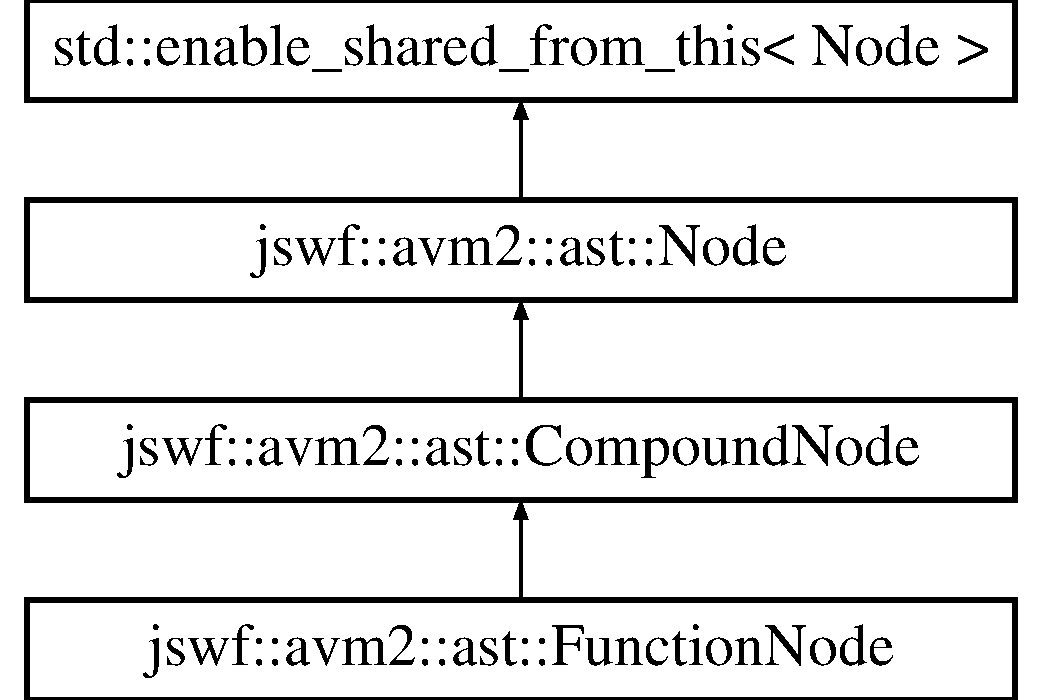
\includegraphics[height=4.000000cm]{classjswf_1_1avm2_1_1ast_1_1_function_node}
\end{center}
\end{figure}
\subsection*{Public Member Functions}
\begin{DoxyCompactItemize}
\item 
\hypertarget{classjswf_1_1avm2_1_1ast_1_1_function_node_a8039437e464a8e6d2e370971b1850dff}{{\bfseries Function\+Node} (\hyperlink{structjswf_1_1avm2_1_1_method_info}{Method\+Info} $\ast$method, std\+::string name)}\label{classjswf_1_1avm2_1_1ast_1_1_function_node_a8039437e464a8e6d2e370971b1850dff}

\item 
\hypertarget{classjswf_1_1avm2_1_1ast_1_1_function_node_ab9627242a660aca73ca75252a78ae0b9}{virtual std\+::string {\bfseries to\+String} ()}\label{classjswf_1_1avm2_1_1ast_1_1_function_node_ab9627242a660aca73ca75252a78ae0b9}

\item 
\hypertarget{classjswf_1_1avm2_1_1ast_1_1_function_node_a3a88a3fb8cacaa78f2f5472659f30419}{virtual std\+::string {\bfseries to\+Intended\+String} (int intend)}\label{classjswf_1_1avm2_1_1ast_1_1_function_node_a3a88a3fb8cacaa78f2f5472659f30419}

\end{DoxyCompactItemize}
\subsection*{Public Attributes}
\begin{DoxyCompactItemize}
\item 
\hypertarget{classjswf_1_1avm2_1_1ast_1_1_function_node_a05b7fd3a985147d18c03182f41103196}{\hyperlink{structjswf_1_1avm2_1_1_method_info}{Method\+Info} $\ast$ {\bfseries method}}\label{classjswf_1_1avm2_1_1ast_1_1_function_node_a05b7fd3a985147d18c03182f41103196}

\item 
\hypertarget{classjswf_1_1avm2_1_1ast_1_1_function_node_a74b195c0bb260375dab6e195b7756d4c}{std\+::string {\bfseries name}}\label{classjswf_1_1avm2_1_1ast_1_1_function_node_a74b195c0bb260375dab6e195b7756d4c}

\end{DoxyCompactItemize}


\subsection{Detailed Description}
Describes a function literal. 

The documentation for this class was generated from the following file\+:\begin{DoxyCompactItemize}
\item 
jswf/avm2/ast/Node.\+h\end{DoxyCompactItemize}

\hypertarget{classjswf_1_1avm2_1_1_function_object}{\section{jswf\+:\+:avm2\+:\+:Function\+Object Class Reference}
\label{classjswf_1_1avm2_1_1_function_object}\index{jswf\+::avm2\+::\+Function\+Object@{jswf\+::avm2\+::\+Function\+Object}}
}


Represents a {\ttfamily function() \{\}} that was created using {\ttfamily newfunction}.  




{\ttfamily \#include $<$Object.\+h$>$}

Inheritance diagram for jswf\+:\+:avm2\+:\+:Function\+Object\+:\begin{figure}[H]
\begin{center}
\leavevmode
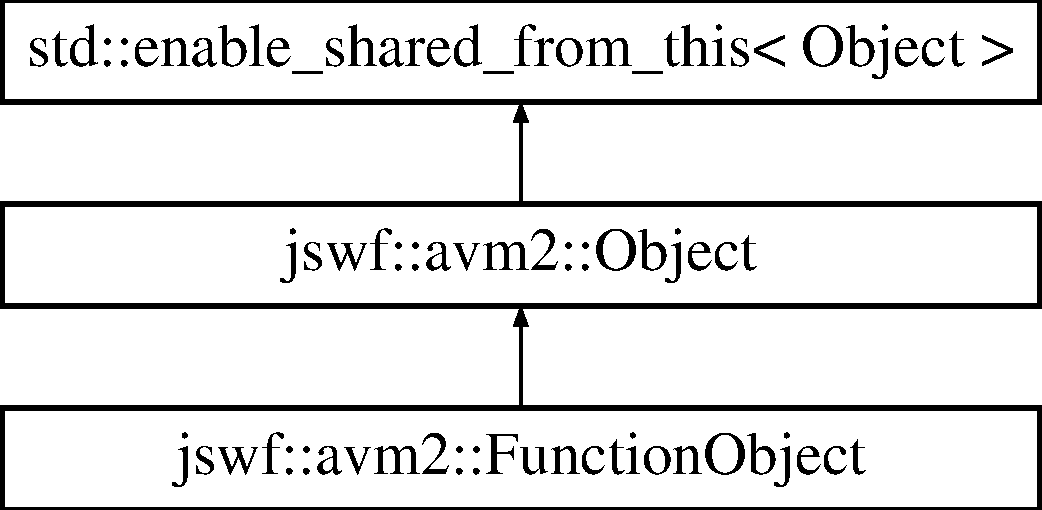
\includegraphics[height=3.000000cm]{classjswf_1_1avm2_1_1_function_object}
\end{center}
\end{figure}
\subsection*{Public Member Functions}
\begin{DoxyCompactItemize}
\item 
\hypertarget{classjswf_1_1avm2_1_1_function_object_a7e1b1e1fe5f501de5637d570fc16ff85}{{\bfseries Function\+Object} (\hyperlink{classjswf_1_1avm2_1_1_v_m}{V\+M} $\ast$vm, \hyperlink{structjswf_1_1avm2_1_1_method_info}{Method\+Info} $\ast$value)}\label{classjswf_1_1avm2_1_1_function_object_a7e1b1e1fe5f501de5637d570fc16ff85}

\item 
std\+::string \hyperlink{classjswf_1_1avm2_1_1_function_object_ac55cd266dc4433d40bb2fcae8bf06d6e}{coerce\+\_\+s} () const 
\begin{DoxyCompactList}\small\item\em Converts to {\ttfamily std\+::string} (E\+C\+M\+A-\/262, section 9.\+8 {\itshape To\+String}) \end{DoxyCompactList}\item 
\hypertarget{classjswf_1_1avm2_1_1_function_object_a4728e9735e1143835de32e56808fd0c0}{Object\+Ptr {\bfseries ecma\+Call} (\hyperlink{classjswf_1_1avm2_1_1_v_m}{V\+M} \&vm, std\+::vector$<$ Object\+Ptr $>$ \&args) const }\label{classjswf_1_1avm2_1_1_function_object_a4728e9735e1143835de32e56808fd0c0}

\end{DoxyCompactItemize}
\subsection*{Public Attributes}
\begin{DoxyCompactItemize}
\item 
\hypertarget{classjswf_1_1avm2_1_1_function_object_ae09a10d691526c9049f6e12e6ae7ccd9}{\hyperlink{structjswf_1_1avm2_1_1_method_info}{Method\+Info} $\ast$ {\bfseries value}}\label{classjswf_1_1avm2_1_1_function_object_ae09a10d691526c9049f6e12e6ae7ccd9}

\end{DoxyCompactItemize}
\subsection*{Additional Inherited Members}


\subsection{Detailed Description}
Represents a {\ttfamily function() \{\}} that was created using {\ttfamily newfunction}. 

\subsection{Member Function Documentation}
\hypertarget{classjswf_1_1avm2_1_1_function_object_ac55cd266dc4433d40bb2fcae8bf06d6e}{\index{jswf\+::avm2\+::\+Function\+Object@{jswf\+::avm2\+::\+Function\+Object}!coerce\+\_\+s@{coerce\+\_\+s}}
\index{coerce\+\_\+s@{coerce\+\_\+s}!jswf\+::avm2\+::\+Function\+Object@{jswf\+::avm2\+::\+Function\+Object}}
\subsubsection[{coerce\+\_\+s}]{\setlength{\rightskip}{0pt plus 5cm}std\+::string jswf\+::avm2\+::\+Function\+Object\+::coerce\+\_\+s (
\begin{DoxyParamCaption}
{}
\end{DoxyParamCaption}
) const\hspace{0.3cm}{\ttfamily [inline]}, {\ttfamily [virtual]}}}\label{classjswf_1_1avm2_1_1_function_object_ac55cd266dc4433d40bb2fcae8bf06d6e}


Converts to {\ttfamily std\+::string} (E\+C\+M\+A-\/262, section 9.\+8 {\itshape To\+String}) 

\begin{DoxyRefDesc}{Todo}
\item[\hyperlink{todo__todo000007}{Todo}]Implement 9.\+8.\+1 \end{DoxyRefDesc}


Reimplemented from \hyperlink{classjswf_1_1avm2_1_1_object_a69b39776062acaccd2cd2b5a1f937c9d}{jswf\+::avm2\+::\+Object}.



The documentation for this class was generated from the following files\+:\begin{DoxyCompactItemize}
\item 
jswf/avm2/Object.\+h\item 
jswf/avm2/Object.\+cpp\end{DoxyCompactItemize}

\hypertarget{structjswf_1_1avm2_1_1_function_trait_info}{\section{jswf\+:\+:avm2\+:\+:Function\+Trait\+Info Struct Reference}
\label{structjswf_1_1avm2_1_1_function_trait_info}\index{jswf\+::avm2\+::\+Function\+Trait\+Info@{jswf\+::avm2\+::\+Function\+Trait\+Info}}
}
Inheritance diagram for jswf\+:\+:avm2\+:\+:Function\+Trait\+Info\+:\begin{figure}[H]
\begin{center}
\leavevmode
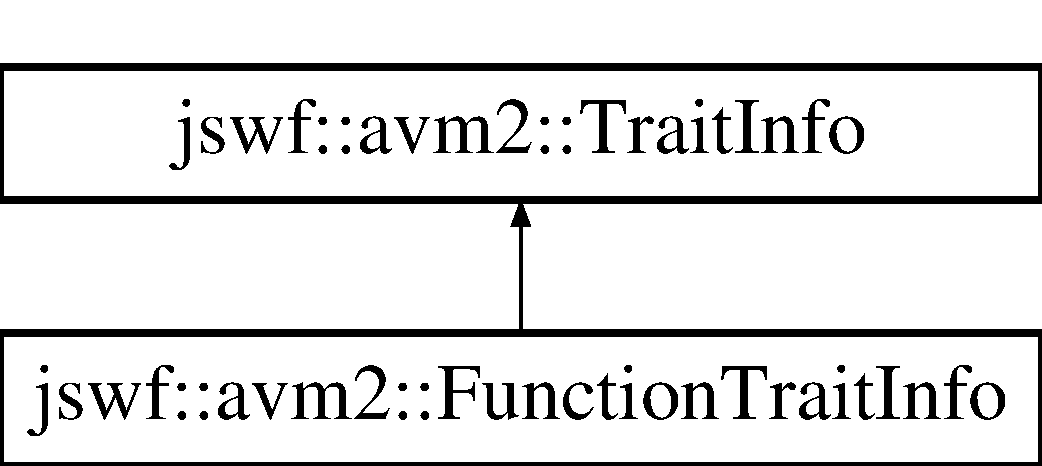
\includegraphics[height=2.000000cm]{structjswf_1_1avm2_1_1_function_trait_info}
\end{center}
\end{figure}
\subsection*{Public Attributes}
\begin{DoxyCompactItemize}
\item 
\hypertarget{structjswf_1_1avm2_1_1_function_trait_info_a44eb1f8750542e2a1c2a777ed5b6922d}{\hyperlink{namespacejswf_aa10d9ddca2a6a5debdc261dfae3d1117}{u30\+\_\+t} {\bfseries slot\+Id}}\label{structjswf_1_1avm2_1_1_function_trait_info_a44eb1f8750542e2a1c2a777ed5b6922d}

\item 
\hypertarget{structjswf_1_1avm2_1_1_function_trait_info_a9a2b872427c231cc6b848ed17ac58f18}{\hyperlink{structjswf_1_1avm2_1_1_method_info}{Method\+Info} $\ast$ {\bfseries method\+Info}}\label{structjswf_1_1avm2_1_1_function_trait_info_a9a2b872427c231cc6b848ed17ac58f18}

\end{DoxyCompactItemize}
\subsection*{Additional Inherited Members}


The documentation for this struct was generated from the following file\+:\begin{DoxyCompactItemize}
\item 
jswf/avm2/Trait\+Info.\+h\end{DoxyCompactItemize}

\hypertarget{classjswf_1_1io_1_1_generic_reader}{\section{jswf\+:\+:io\+:\+:Generic\+Reader Class Reference}
\label{classjswf_1_1io_1_1_generic_reader}\index{jswf\+::io\+::\+Generic\+Reader@{jswf\+::io\+::\+Generic\+Reader}}
}


Servers as reader for primitive data-\/types like integers, doubles and strings.  




{\ttfamily \#include $<$Generic\+Reader.\+h$>$}

Inheritance diagram for jswf\+:\+:io\+:\+:Generic\+Reader\+:\begin{figure}[H]
\begin{center}
\leavevmode
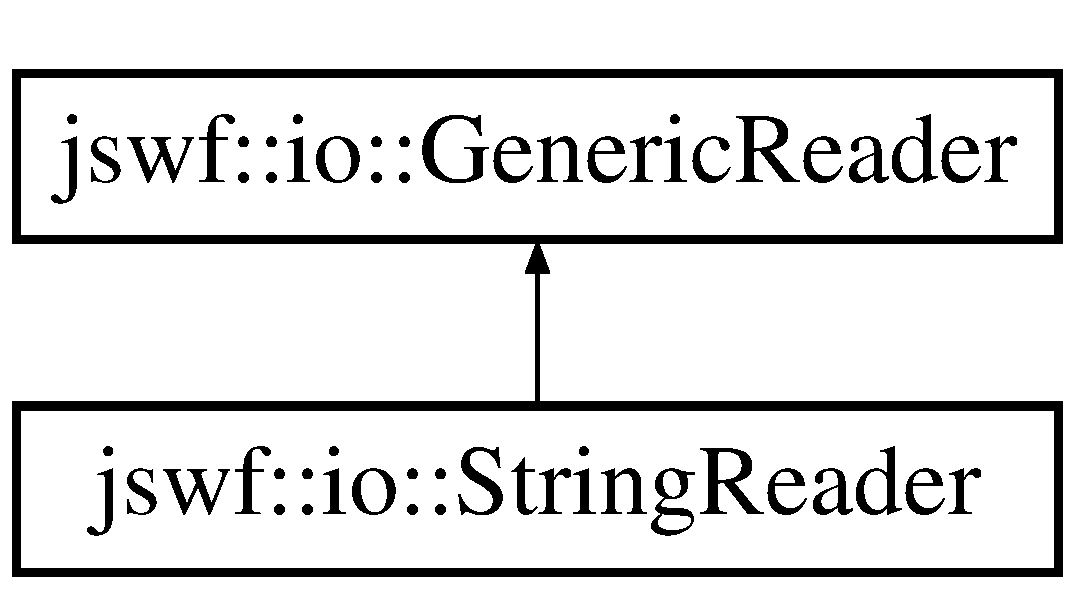
\includegraphics[height=2.000000cm]{classjswf_1_1io_1_1_generic_reader}
\end{center}
\end{figure}
\subsection*{Public Member Functions}
\begin{DoxyCompactItemize}
\item 
\hypertarget{classjswf_1_1io_1_1_generic_reader_a5ed096def8d74916ee47b7537842b4da}{virtual \hyperlink{namespacejswf_a3458b3040189121ea8ffc0bdfd3e32ee}{u8\+\_\+t} \hyperlink{classjswf_1_1io_1_1_generic_reader_a5ed096def8d74916ee47b7537842b4da}{read\+U8} ()=0}\label{classjswf_1_1io_1_1_generic_reader_a5ed096def8d74916ee47b7537842b4da}

\begin{DoxyCompactList}\small\item\em Reads a byte-\/aligned 8-\/bit unsigned integer. \end{DoxyCompactList}\item 
\hypertarget{classjswf_1_1io_1_1_generic_reader_a548b8e690f367ede657fa6227e49c6b9}{virtual \hyperlink{namespacejswf_a68db00e879e7d4a42c18e20dcea75292}{u16\+\_\+t} \hyperlink{classjswf_1_1io_1_1_generic_reader_a548b8e690f367ede657fa6227e49c6b9}{read\+U16} ()=0}\label{classjswf_1_1io_1_1_generic_reader_a548b8e690f367ede657fa6227e49c6b9}

\begin{DoxyCompactList}\small\item\em Reads a byte-\/aligned 16-\/bit unsigned integer (little endian) \end{DoxyCompactList}\item 
\hypertarget{classjswf_1_1io_1_1_generic_reader_a76a50b1e5706a02d044feff14cc3d16e}{virtual \hyperlink{namespacejswf_ae68dd480b6437e9a20db7b004283a466}{u32\+\_\+t} \hyperlink{classjswf_1_1io_1_1_generic_reader_a76a50b1e5706a02d044feff14cc3d16e}{read\+U32} ()=0}\label{classjswf_1_1io_1_1_generic_reader_a76a50b1e5706a02d044feff14cc3d16e}

\begin{DoxyCompactList}\small\item\em Reads a byte-\/aligned 32-\/bit unsigned integer (little endian) \end{DoxyCompactList}\item 
\hypertarget{classjswf_1_1io_1_1_generic_reader_a764f46418f5aff7ba3d79264d136479e}{virtual \hyperlink{namespacejswf_a75cd7aa1b422e7e8b2883bcececdc5a2}{s8\+\_\+t} \hyperlink{classjswf_1_1io_1_1_generic_reader_a764f46418f5aff7ba3d79264d136479e}{read\+S8} ()}\label{classjswf_1_1io_1_1_generic_reader_a764f46418f5aff7ba3d79264d136479e}

\begin{DoxyCompactList}\small\item\em Reads a byte-\/aligned 8-\/bit signed integer. \end{DoxyCompactList}\item 
\hypertarget{classjswf_1_1io_1_1_generic_reader_a91f932a0cbe82712697b728d70f5d861}{virtual \hyperlink{namespacejswf_a229666eb55cfe287190dad8c25f58f02}{s16\+\_\+t} \hyperlink{classjswf_1_1io_1_1_generic_reader_a91f932a0cbe82712697b728d70f5d861}{read\+S16} ()}\label{classjswf_1_1io_1_1_generic_reader_a91f932a0cbe82712697b728d70f5d861}

\begin{DoxyCompactList}\small\item\em Reads a byte-\/aligned 16-\/bit signed integer (little endian) \end{DoxyCompactList}\item 
\hypertarget{classjswf_1_1io_1_1_generic_reader_a50b8f5f4aa979c196e6a7f3c34861617}{virtual \hyperlink{namespacejswf_a19b2a5980fe3b05994a2127a3c7e0521}{s32\+\_\+t} \hyperlink{classjswf_1_1io_1_1_generic_reader_a50b8f5f4aa979c196e6a7f3c34861617}{read\+S32} ()}\label{classjswf_1_1io_1_1_generic_reader_a50b8f5f4aa979c196e6a7f3c34861617}

\begin{DoxyCompactList}\small\item\em Reads a byte-\/aligned 32-\/bit signed integer (little endian) \end{DoxyCompactList}\item 
\hypertarget{classjswf_1_1io_1_1_generic_reader_aebaf827aa7ce24f1e5bf8f599938eda0}{virtual \hyperlink{namespacejswf_a755127d61081aa8af105eb800aa2c1ec}{string} \hyperlink{classjswf_1_1io_1_1_generic_reader_aebaf827aa7ce24f1e5bf8f599938eda0}{read\+String} ()=0}\label{classjswf_1_1io_1_1_generic_reader_aebaf827aa7ce24f1e5bf8f599938eda0}

\begin{DoxyCompactList}\small\item\em Reads a N\+U\+L-\/terminated string (C-\/string) \end{DoxyCompactList}\item 
\hypertarget{classjswf_1_1io_1_1_generic_reader_acc4f05833b09bcaf2baec3ba46ec0477}{virtual \hyperlink{namespacejswf_a755127d61081aa8af105eb800aa2c1ec}{string} \hyperlink{classjswf_1_1io_1_1_generic_reader_acc4f05833b09bcaf2baec3ba46ec0477}{read\+String} (size\+\_\+t length)=0}\label{classjswf_1_1io_1_1_generic_reader_acc4f05833b09bcaf2baec3ba46ec0477}

\begin{DoxyCompactList}\small\item\em Reads a string of a given length. \end{DoxyCompactList}\item 
\hypertarget{classjswf_1_1io_1_1_generic_reader_aa1445404182efbda9c46b6c9b9ea9c74}{virtual \hyperlink{namespacejswf_a38f034ab4371db2c8aee66e1c92b5bc7}{ub\+\_\+t} \hyperlink{classjswf_1_1io_1_1_generic_reader_aa1445404182efbda9c46b6c9b9ea9c74}{read\+U\+B} (uint8\+\_\+t nbits)=0}\label{classjswf_1_1io_1_1_generic_reader_aa1445404182efbda9c46b6c9b9ea9c74}

\begin{DoxyCompactList}\small\item\em Reads a unsigned bit-\/field of length {\ttfamily nbits} \end{DoxyCompactList}\item 
\hypertarget{classjswf_1_1io_1_1_generic_reader_ab969b53faac7ff67b4fe8144d6d27c78}{virtual \hyperlink{namespacejswf_aa56b2b764590a9e19a5e66693364aceb}{sb\+\_\+t} \hyperlink{classjswf_1_1io_1_1_generic_reader_ab969b53faac7ff67b4fe8144d6d27c78}{read\+S\+B} (uint8\+\_\+t nbits)}\label{classjswf_1_1io_1_1_generic_reader_ab969b53faac7ff67b4fe8144d6d27c78}

\begin{DoxyCompactList}\small\item\em Reads a signed bit-\/field of length {\ttfamily nbits}, sign-\/extends to fill {\ttfamily sb\+\_\+t} \end{DoxyCompactList}\item 
\hypertarget{classjswf_1_1io_1_1_generic_reader_a82a78364fdd97b6eff791e0a768e1d46}{virtual \hyperlink{namespacejswf_a419cb8aa8b625074e6753d189783b2f4}{fb\+\_\+t} \hyperlink{classjswf_1_1io_1_1_generic_reader_a82a78364fdd97b6eff791e0a768e1d46}{read\+F\+B} (uint8\+\_\+t nbits)}\label{classjswf_1_1io_1_1_generic_reader_a82a78364fdd97b6eff791e0a768e1d46}

\begin{DoxyCompactList}\small\item\em Reads a F\+I\+X\+E\+D8.\+8. \end{DoxyCompactList}\item 
\hypertarget{classjswf_1_1io_1_1_generic_reader_ab9e82ef9f3e31b2e9a4c7578fc005483}{virtual void \hyperlink{classjswf_1_1io_1_1_generic_reader_ab9e82ef9f3e31b2e9a4c7578fc005483}{align} (uint8\+\_\+t bytes)=0}\label{classjswf_1_1io_1_1_generic_reader_ab9e82ef9f3e31b2e9a4c7578fc005483}

\begin{DoxyCompactList}\small\item\em Aligns the reader to a multiple of 'bytes', resets bit-\/position. \end{DoxyCompactList}\item 
\hypertarget{classjswf_1_1io_1_1_generic_reader_a35ef3dad6e2c5b36a2a3214a9b0e4272}{virtual \hyperlink{namespacejswf_a755127d61081aa8af105eb800aa2c1ec}{string} \hyperlink{classjswf_1_1io_1_1_generic_reader_a35ef3dad6e2c5b36a2a3214a9b0e4272}{read\+Remaining} ()=0}\label{classjswf_1_1io_1_1_generic_reader_a35ef3dad6e2c5b36a2a3214a9b0e4272}

\begin{DoxyCompactList}\small\item\em Reads all remaining bytes (bit-\/position rounded up) \end{DoxyCompactList}\item 
\hypertarget{classjswf_1_1io_1_1_generic_reader_a11588c67c62d3fa46690a024cb0405ff}{virtual bool \hyperlink{classjswf_1_1io_1_1_generic_reader_a11588c67c62d3fa46690a024cb0405ff}{eof} ()=0}\label{classjswf_1_1io_1_1_generic_reader_a11588c67c62d3fa46690a024cb0405ff}

\begin{DoxyCompactList}\small\item\em Returns true if the end of stream is reached, false otherwise. \end{DoxyCompactList}\item 
\hypertarget{classjswf_1_1io_1_1_generic_reader_ac09240cd1e70fe0e020a301217d4fb2b}{virtual \hyperlink{namespacejswf_a19b2a5980fe3b05994a2127a3c7e0521}{s32\+\_\+t} \hyperlink{classjswf_1_1io_1_1_generic_reader_ac09240cd1e70fe0e020a301217d4fb2b}{read\+S24} ()=0}\label{classjswf_1_1io_1_1_generic_reader_ac09240cd1e70fe0e020a301217d4fb2b}

\begin{DoxyCompactList}\small\item\em Reads a byte-\/aligned 24-\/bit unsigned integer (little endian) \end{DoxyCompactList}\item 
\hypertarget{classjswf_1_1io_1_1_generic_reader_ae93752df73846ca760e748f22612c88f}{virtual \hyperlink{namespacejswf_ae68dd480b6437e9a20db7b004283a466}{u32\+\_\+t} \hyperlink{classjswf_1_1io_1_1_generic_reader_ae93752df73846ca760e748f22612c88f}{read\+V\+U30} ()=0}\label{classjswf_1_1io_1_1_generic_reader_ae93752df73846ca760e748f22612c88f}

\begin{DoxyCompactList}\small\item\em Reads a byte-\/aligned, variable-\/length encoded 30-\/bit unsigned integer. \end{DoxyCompactList}\item 
\hypertarget{classjswf_1_1io_1_1_generic_reader_ade48eb74c708f1611c74aaa787da2754}{virtual \hyperlink{namespacejswf_ae68dd480b6437e9a20db7b004283a466}{u32\+\_\+t} \hyperlink{classjswf_1_1io_1_1_generic_reader_ade48eb74c708f1611c74aaa787da2754}{read\+V\+U32} ()=0}\label{classjswf_1_1io_1_1_generic_reader_ade48eb74c708f1611c74aaa787da2754}

\begin{DoxyCompactList}\small\item\em Reads a byte-\/aligned, variable-\/length encoded 32-\/bit unsigned integer. \end{DoxyCompactList}\item 
\hypertarget{classjswf_1_1io_1_1_generic_reader_abff66404e36d68224b1e222c6632115b}{virtual \hyperlink{namespacejswf_a19b2a5980fe3b05994a2127a3c7e0521}{s32\+\_\+t} \hyperlink{classjswf_1_1io_1_1_generic_reader_abff66404e36d68224b1e222c6632115b}{read\+V\+S32} ()=0}\label{classjswf_1_1io_1_1_generic_reader_abff66404e36d68224b1e222c6632115b}

\begin{DoxyCompactList}\small\item\em Reads a byte-\/aligned, variable-\/length encoded 32-\/bit signed integer. \end{DoxyCompactList}\item 
\hypertarget{classjswf_1_1io_1_1_generic_reader_a56ad5cbf914f67d3633318093dfcb0d3}{virtual \hyperlink{namespacejswf_acfbb3c7c9fbb807e233387995eb76a96}{d64\+\_\+t} \hyperlink{classjswf_1_1io_1_1_generic_reader_a56ad5cbf914f67d3633318093dfcb0d3}{read\+D64} ()=0}\label{classjswf_1_1io_1_1_generic_reader_a56ad5cbf914f67d3633318093dfcb0d3}

\begin{DoxyCompactList}\small\item\em Reads a I\+E\+E-\/754 double-\/precision floating point number. \end{DoxyCompactList}\end{DoxyCompactItemize}
\subsection*{Public Attributes}
\begin{DoxyCompactItemize}
\item 
size\+\_\+t \hyperlink{classjswf_1_1io_1_1_generic_reader_a29dcfa1317485ea04e6caef568e803ce}{pos} = 0
\begin{DoxyCompactList}\small\item\em Our current byte position. \end{DoxyCompactList}\item 
\hypertarget{classjswf_1_1io_1_1_generic_reader_ab877457369b0cc359c724547c757ec7b}{uint8\+\_\+t \hyperlink{classjswf_1_1io_1_1_generic_reader_ab877457369b0cc359c724547c757ec7b}{bitpos} = 0}\label{classjswf_1_1io_1_1_generic_reader_ab877457369b0cc359c724547c757ec7b}

\begin{DoxyCompactList}\small\item\em Our current bit position \mbox{[}0;8) inside the byte position. \end{DoxyCompactList}\end{DoxyCompactItemize}


\subsection{Detailed Description}
Servers as reader for primitive data-\/types like integers, doubles and strings. 

\subsection{Member Data Documentation}
\hypertarget{classjswf_1_1io_1_1_generic_reader_a29dcfa1317485ea04e6caef568e803ce}{\index{jswf\+::io\+::\+Generic\+Reader@{jswf\+::io\+::\+Generic\+Reader}!pos@{pos}}
\index{pos@{pos}!jswf\+::io\+::\+Generic\+Reader@{jswf\+::io\+::\+Generic\+Reader}}
\subsubsection[{pos}]{\setlength{\rightskip}{0pt plus 5cm}size\+\_\+t jswf\+::io\+::\+Generic\+Reader\+::pos = 0}}\label{classjswf_1_1io_1_1_generic_reader_a29dcfa1317485ea04e6caef568e803ce}


Our current byte position. 

\begin{DoxyRefDesc}{Todo}
\item[\hyperlink{todo__todo000022}{Todo}]Protected with optional seek. \end{DoxyRefDesc}


The documentation for this class was generated from the following files\+:\begin{DoxyCompactItemize}
\item 
jswf/io/\hyperlink{_generic_reader_8h}{Generic\+Reader.\+h}\item 
jswf/io/Generic\+Reader.\+cpp\end{DoxyCompactItemize}

\hypertarget{classjswf_1_1flash_1_1styles_1_1_gradient_fill_style}{\section{jswf\+:\+:flash\+:\+:styles\+:\+:Gradient\+Fill\+Style Class Reference}
\label{classjswf_1_1flash_1_1styles_1_1_gradient_fill_style}\index{jswf\+::flash\+::styles\+::\+Gradient\+Fill\+Style@{jswf\+::flash\+::styles\+::\+Gradient\+Fill\+Style}}
}
Inheritance diagram for jswf\+:\+:flash\+:\+:styles\+:\+:Gradient\+Fill\+Style\+:\begin{figure}[H]
\begin{center}
\leavevmode
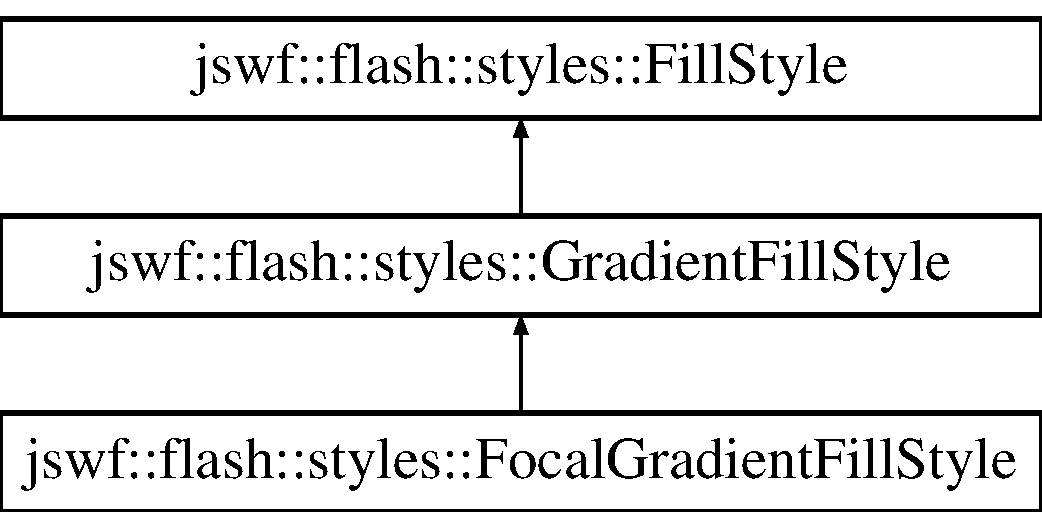
\includegraphics[height=3.000000cm]{classjswf_1_1flash_1_1styles_1_1_gradient_fill_style}
\end{center}
\end{figure}
\subsection*{Public Attributes}
\begin{DoxyCompactItemize}
\item 
\hypertarget{classjswf_1_1flash_1_1styles_1_1_gradient_fill_style_a2cb7b9a0548773fa84c81bee49c63082}{uint8\+\_\+t {\bfseries spread\+Mode}}\label{classjswf_1_1flash_1_1styles_1_1_gradient_fill_style_a2cb7b9a0548773fa84c81bee49c63082}

\item 
\hypertarget{classjswf_1_1flash_1_1styles_1_1_gradient_fill_style_aafed92563fe46687c170e78a06ef501f}{uint8\+\_\+t {\bfseries interpolation\+Mode}}\label{classjswf_1_1flash_1_1styles_1_1_gradient_fill_style_aafed92563fe46687c170e78a06ef501f}

\item 
\hypertarget{classjswf_1_1flash_1_1styles_1_1_gradient_fill_style_a79886d8ef621456a790c8489248e5087}{\hyperlink{structjswf_1_1flash_1_1_matrix}{Matrix} {\bfseries matrix}}\label{classjswf_1_1flash_1_1styles_1_1_gradient_fill_style_a79886d8ef621456a790c8489248e5087}

\item 
\hypertarget{classjswf_1_1flash_1_1styles_1_1_gradient_fill_style_a2700c16bb045c3ff52ca3f11c4dda30b}{bool {\bfseries is\+Radial} = false}\label{classjswf_1_1flash_1_1styles_1_1_gradient_fill_style_a2700c16bb045c3ff52ca3f11c4dda30b}

\item 
\hypertarget{classjswf_1_1flash_1_1styles_1_1_gradient_fill_style_a40285054cf588f639af30500aa4067ce}{std\+::vector$<$ \hyperlink{structjswf_1_1flash_1_1styles_1_1_gradient_stop}{Gradient\+Stop} $>$ {\bfseries stops}}\label{classjswf_1_1flash_1_1styles_1_1_gradient_fill_style_a40285054cf588f639af30500aa4067ce}

\end{DoxyCompactItemize}


The documentation for this class was generated from the following file\+:\begin{DoxyCompactItemize}
\item 
jswf/flash/styles/Fill\+Style.\+h\end{DoxyCompactItemize}

\hypertarget{structjswf_1_1flash_1_1styles_1_1_gradient_stop}{\section{jswf\+:\+:flash\+:\+:styles\+:\+:Gradient\+Stop Struct Reference}
\label{structjswf_1_1flash_1_1styles_1_1_gradient_stop}\index{jswf\+::flash\+::styles\+::\+Gradient\+Stop@{jswf\+::flash\+::styles\+::\+Gradient\+Stop}}
}
\subsection*{Public Attributes}
\begin{DoxyCompactItemize}
\item 
\hypertarget{structjswf_1_1flash_1_1styles_1_1_gradient_stop_ac2b03dd84d1a6514b218eff43705a0f9}{uint8\+\_\+t {\bfseries ratio}}\label{structjswf_1_1flash_1_1styles_1_1_gradient_stop_ac2b03dd84d1a6514b218eff43705a0f9}

\item 
\hypertarget{structjswf_1_1flash_1_1styles_1_1_gradient_stop_a64b9111ac28850afd2ce19d0bb5538ca}{\hyperlink{structjswf_1_1flash_1_1_r_g_b_a}{R\+G\+B\+A} {\bfseries color}}\label{structjswf_1_1flash_1_1styles_1_1_gradient_stop_a64b9111ac28850afd2ce19d0bb5538ca}

\end{DoxyCompactItemize}


The documentation for this struct was generated from the following file\+:\begin{DoxyCompactItemize}
\item 
jswf/flash/styles/Fill\+Style.\+h\end{DoxyCompactItemize}

\hypertarget{structjswf_1_1flash_1_1_header}{\section{jswf\+:\+:flash\+:\+:Header Struct Reference}
\label{structjswf_1_1flash_1_1_header}\index{jswf\+::flash\+::\+Header@{jswf\+::flash\+::\+Header}}
}


Represents the {\ttfamily H\+E\+A\+D\+E\+R} record.  




{\ttfamily \#include $<$Header.\+h$>$}

\subsection*{Public Attributes}
\begin{DoxyCompactItemize}
\item 
\hypertarget{structjswf_1_1flash_1_1_header_aeeec53edb1da8f04f91c0dfc999ce02b}{\hyperlink{structjswf_1_1flash_1_1_compression_a393e4fe7bb01f081e0c1d1d009c22c2a}{Compression\+::\+Enum} \hyperlink{structjswf_1_1flash_1_1_header_aeeec53edb1da8f04f91c0dfc999ce02b}{compression}}\label{structjswf_1_1flash_1_1_header_aeeec53edb1da8f04f91c0dfc999ce02b}

\begin{DoxyCompactList}\small\item\em The compression used for the file. \end{DoxyCompactList}\item 
\hypertarget{structjswf_1_1flash_1_1_header_afee43d7f58d6e6f9274fd238bf33619e}{version\+\_\+t \hyperlink{structjswf_1_1flash_1_1_header_afee43d7f58d6e6f9274fd238bf33619e}{version}}\label{structjswf_1_1flash_1_1_header_afee43d7f58d6e6f9274fd238bf33619e}

\begin{DoxyCompactList}\small\item\em The Flash version that this file targets. \end{DoxyCompactList}\item 
\hypertarget{structjswf_1_1flash_1_1_header_a6886af043400e1d2a5300e7110e88de0}{uint32\+\_\+t \hyperlink{structjswf_1_1flash_1_1_header_a6886af043400e1d2a5300e7110e88de0}{file\+Size}}\label{structjswf_1_1flash_1_1_header_a6886af043400e1d2a5300e7110e88de0}

\begin{DoxyCompactList}\small\item\em The total file size (including header) after decompression. \end{DoxyCompactList}\item 
\hypertarget{structjswf_1_1flash_1_1_header_a2d609e0a85bd0eef4a2b79e7cd793789}{uint16\+\_\+t \hyperlink{structjswf_1_1flash_1_1_header_a2d609e0a85bd0eef4a2b79e7cd793789}{frame\+Rate}}\label{structjswf_1_1flash_1_1_header_a2d609e0a85bd0eef4a2b79e7cd793789}

\begin{DoxyCompactList}\small\item\em The frame rate of this file in 1/256 F\+P\+S. \end{DoxyCompactList}\item 
\hypertarget{structjswf_1_1flash_1_1_header_ab687d679b8c9f543571913b98a0f6795}{uint16\+\_\+t \hyperlink{structjswf_1_1flash_1_1_header_ab687d679b8c9f543571913b98a0f6795}{frame\+Count}}\label{structjswf_1_1flash_1_1_header_ab687d679b8c9f543571913b98a0f6795}

\begin{DoxyCompactList}\small\item\em The count of frames for the main timeline. \end{DoxyCompactList}\item 
\hypertarget{structjswf_1_1flash_1_1_header_a458a074681b52632fe31faa33b760773}{\hyperlink{structjswf_1_1flash_1_1_rect}{Rect} \hyperlink{structjswf_1_1flash_1_1_header_a458a074681b52632fe31faa33b760773}{rect}}\label{structjswf_1_1flash_1_1_header_a458a074681b52632fe31faa33b760773}

\begin{DoxyCompactList}\small\item\em The dimensions of the file in {\ttfamily twips} \end{DoxyCompactList}\end{DoxyCompactItemize}


\subsection{Detailed Description}
Represents the {\ttfamily H\+E\+A\+D\+E\+R} record. 

The documentation for this struct was generated from the following file\+:\begin{DoxyCompactItemize}
\item 
jswf/flash/Header.\+h\end{DoxyCompactItemize}

\hypertarget{classjswf_1_1avm2_1_1_i_constant_source}{\section{jswf\+:\+:avm2\+:\+:I\+Constant\+Source$<$ T $>$ Class Template Reference}
\label{classjswf_1_1avm2_1_1_i_constant_source}\index{jswf\+::avm2\+::\+I\+Constant\+Source$<$ T $>$@{jswf\+::avm2\+::\+I\+Constant\+Source$<$ T $>$}}
}
\subsection*{Public Member Functions}
\begin{DoxyCompactItemize}
\item 
\hypertarget{classjswf_1_1avm2_1_1_i_constant_source_a32505ebb896dbfcdca660187f2cc95c9}{virtual std\+::shared\+\_\+ptr$<$ T $>$ {\bfseries get\+Pool\+Constant} (Constant\+Kind\+::\+Enum kind, \hyperlink{classjswf_1_1avm2_1_1_a_b_c_file}{A\+B\+C\+File} $\ast$file, \hyperlink{namespacejswf_aa10d9ddca2a6a5debdc261dfae3d1117}{u30\+\_\+t} index)=0}\label{classjswf_1_1avm2_1_1_i_constant_source_a32505ebb896dbfcdca660187f2cc95c9}

\item 
\hypertarget{classjswf_1_1avm2_1_1_i_constant_source_abd4ab71644db29813b51f627c5259528}{virtual std\+::shared\+\_\+ptr$<$ T $>$ {\bfseries get\+Constant} (Constant\+Kind\+::\+Enum kind)=0}\label{classjswf_1_1avm2_1_1_i_constant_source_abd4ab71644db29813b51f627c5259528}

\item 
\hypertarget{classjswf_1_1avm2_1_1_i_constant_source_a99da62daf2d81a529f2127a3c9cfedf1}{virtual std\+::shared\+\_\+ptr$<$ T $>$ {\bfseries get\+Immediate\+Constant} (Constant\+Kind\+::\+Enum kind, int32\+\_\+t imm)=0}\label{classjswf_1_1avm2_1_1_i_constant_source_a99da62daf2d81a529f2127a3c9cfedf1}

\end{DoxyCompactItemize}


The documentation for this class was generated from the following file\+:\begin{DoxyCompactItemize}
\item 
jswf/avm2/Opcode.\+h\end{DoxyCompactItemize}

\hypertarget{structjswf_1_1avm2_1_1_instance_info}{\section{jswf\+:\+:avm2\+:\+:Instance\+Info Struct Reference}
\label{structjswf_1_1avm2_1_1_instance_info}\index{jswf\+::avm2\+::\+Instance\+Info@{jswf\+::avm2\+::\+Instance\+Info}}
}
\subsection*{Public Types}
\begin{DoxyCompactItemize}
\item 
\hypertarget{structjswf_1_1avm2_1_1_instance_info_aacb09d330a2785abddd3b9cb8d2b6074}{enum {\bfseries Flags} \+: u8\+\_\+t \{ {\bfseries Class\+Sealed\+Flag} = 0x01, 
{\bfseries Class\+Final\+Flag} = 0x02, 
{\bfseries Class\+Interface\+Flag} = 0x04, 
{\bfseries Class\+Protected\+Ns\+Flag} = 0x08
 \}}\label{structjswf_1_1avm2_1_1_instance_info_aacb09d330a2785abddd3b9cb8d2b6074}

\end{DoxyCompactItemize}
\subsection*{Public Attributes}
\begin{DoxyCompactItemize}
\item 
\hypertarget{structjswf_1_1avm2_1_1_instance_info_ad13864988ec329dafa299adaf7f92166}{Multiname\+Ptr {\bfseries name}}\label{structjswf_1_1avm2_1_1_instance_info_ad13864988ec329dafa299adaf7f92166}

\item 
\hypertarget{structjswf_1_1avm2_1_1_instance_info_a38f867e63d526149c7d343ca5c61655a}{Multiname\+Ptr {\bfseries super\+Name}}\label{structjswf_1_1avm2_1_1_instance_info_a38f867e63d526149c7d343ca5c61655a}

\item 
\hypertarget{structjswf_1_1avm2_1_1_instance_info_a3a073d319cd66dff46ebb48c9d00d5f1}{Flags {\bfseries flags}}\label{structjswf_1_1avm2_1_1_instance_info_a3a073d319cd66dff46ebb48c9d00d5f1}

\item 
\hypertarget{structjswf_1_1avm2_1_1_instance_info_a9ea1d5f094ff213ff4c5a091e288405f}{Namespace\+Ptr {\bfseries protected\+Ns}}\label{structjswf_1_1avm2_1_1_instance_info_a9ea1d5f094ff213ff4c5a091e288405f}

\item 
\hypertarget{structjswf_1_1avm2_1_1_instance_info_a6189acb4157edacb457337cba4d642ed}{std\+::vector$<$ Multiname\+Ptr $>$ {\bfseries interfaces}}\label{structjswf_1_1avm2_1_1_instance_info_a6189acb4157edacb457337cba4d642ed}

\item 
\hypertarget{structjswf_1_1avm2_1_1_instance_info_a8a30b54bd64c13c057ac9f7cf35ddd0e}{\hyperlink{structjswf_1_1avm2_1_1_method_info}{Method\+Info} $\ast$ {\bfseries initializer}}\label{structjswf_1_1avm2_1_1_instance_info_a8a30b54bd64c13c057ac9f7cf35ddd0e}

\item 
\hypertarget{structjswf_1_1avm2_1_1_instance_info_adbfcf225e4ccdc11f7598457c32b04c1}{std\+::vector$<$ std\+::shared\+\_\+ptr\\*
$<$ \hyperlink{structjswf_1_1avm2_1_1_trait_info}{Trait\+Info} $>$ $>$ {\bfseries traits}}\label{structjswf_1_1avm2_1_1_instance_info_adbfcf225e4ccdc11f7598457c32b04c1}

\end{DoxyCompactItemize}


The documentation for this struct was generated from the following file\+:\begin{DoxyCompactItemize}
\item 
jswf/avm2/A\+B\+C\+File.\+h\end{DoxyCompactItemize}

\hypertarget{classjswf_1_1avm2_1_1ast_1_1_int_node}{\section{jswf\+:\+:avm2\+:\+:ast\+:\+:Int\+Node Class Reference}
\label{classjswf_1_1avm2_1_1ast_1_1_int_node}\index{jswf\+::avm2\+::ast\+::\+Int\+Node@{jswf\+::avm2\+::ast\+::\+Int\+Node}}
}


Describes a node that carries an integer literal.  




{\ttfamily \#include $<$Node.\+h$>$}

Inheritance diagram for jswf\+:\+:avm2\+:\+:ast\+:\+:Int\+Node\+:\begin{figure}[H]
\begin{center}
\leavevmode
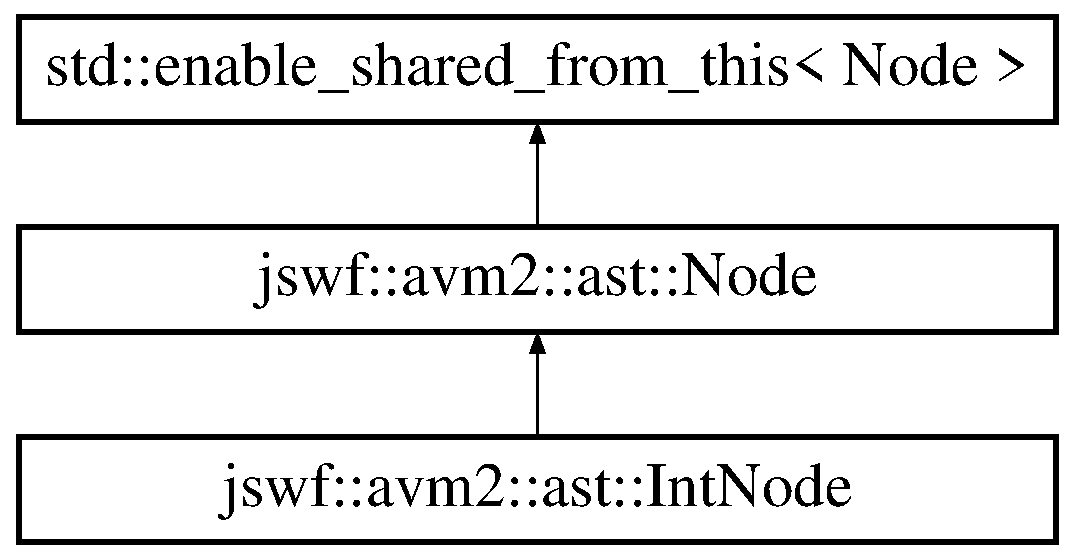
\includegraphics[height=3.000000cm]{classjswf_1_1avm2_1_1ast_1_1_int_node}
\end{center}
\end{figure}
\subsection*{Public Member Functions}
\begin{DoxyCompactItemize}
\item 
\hypertarget{classjswf_1_1avm2_1_1ast_1_1_int_node_aea17b59404788a611adc76798c4c7e33}{{\bfseries Int\+Node} (int v)}\label{classjswf_1_1avm2_1_1ast_1_1_int_node_aea17b59404788a611adc76798c4c7e33}

\item 
\hypertarget{classjswf_1_1avm2_1_1ast_1_1_int_node_a09eae9556ab956d91b4035585d34b743}{virtual std\+::string {\bfseries to\+String} ()}\label{classjswf_1_1avm2_1_1ast_1_1_int_node_a09eae9556ab956d91b4035585d34b743}

\end{DoxyCompactItemize}
\subsection*{Public Attributes}
\begin{DoxyCompactItemize}
\item 
\hypertarget{classjswf_1_1avm2_1_1ast_1_1_int_node_a04c26ec9971a10a08477e24ff21b04ed}{int {\bfseries value}}\label{classjswf_1_1avm2_1_1ast_1_1_int_node_a04c26ec9971a10a08477e24ff21b04ed}

\end{DoxyCompactItemize}


\subsection{Detailed Description}
Describes a node that carries an integer literal. 

The documentation for this class was generated from the following file\+:\begin{DoxyCompactItemize}
\item 
jswf/avm2/ast/Node.\+h\end{DoxyCompactItemize}

\hypertarget{classjswf_1_1flash_1_1tags_1_1_i_tag_for_document}{\section{jswf\+:\+:flash\+:\+:tags\+:\+:I\+Tag\+For\+Document Class Reference}
\label{classjswf_1_1flash_1_1tags_1_1_i_tag_for_document}\index{jswf\+::flash\+::tags\+::\+I\+Tag\+For\+Document@{jswf\+::flash\+::tags\+::\+I\+Tag\+For\+Document}}
}


Interface for {\ttfamily T\+A\+G}s that implement actions to be performed on the \hyperlink{classjswf_1_1flash_1_1_document}{Document}.  




{\ttfamily \#include $<$I\+Tag\+For\+Document.\+h$>$}

Inheritance diagram for jswf\+:\+:flash\+:\+:tags\+:\+:I\+Tag\+For\+Document\+:\begin{figure}[H]
\begin{center}
\leavevmode
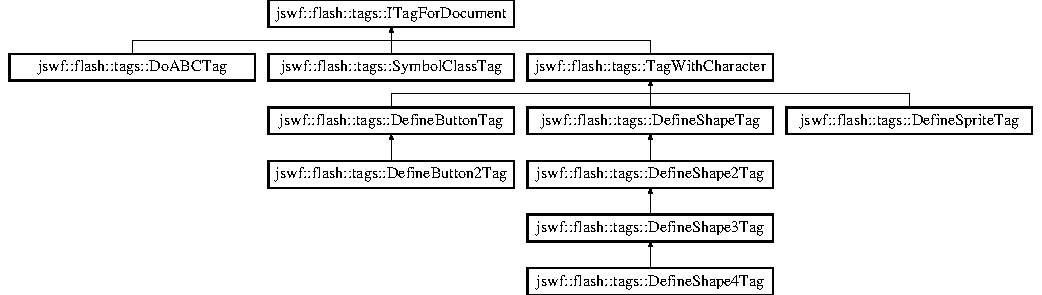
\includegraphics[height=3.962264cm]{classjswf_1_1flash_1_1tags_1_1_i_tag_for_document}
\end{center}
\end{figure}
\subsection*{Public Member Functions}
\begin{DoxyCompactItemize}
\item 
\hypertarget{classjswf_1_1flash_1_1tags_1_1_i_tag_for_document_a514c81dde789ab9e919ebd4873502903}{virtual void {\bfseries apply\+To\+Document} (\hyperlink{classjswf_1_1flash_1_1_document}{Document} \&document)=0}\label{classjswf_1_1flash_1_1tags_1_1_i_tag_for_document_a514c81dde789ab9e919ebd4873502903}

\end{DoxyCompactItemize}


\subsection{Detailed Description}
Interface for {\ttfamily T\+A\+G}s that implement actions to be performed on the \hyperlink{classjswf_1_1flash_1_1_document}{Document}. 

The documentation for this class was generated from the following file\+:\begin{DoxyCompactItemize}
\item 
jswf/flash/tags/\hyperlink{_i_tag_for_document_8h}{I\+Tag\+For\+Document.\+h}\end{DoxyCompactItemize}

\hypertarget{classjswf_1_1flash_1_1tags_1_1_i_tag_for_sprite}{\section{jswf\+:\+:flash\+:\+:tags\+:\+:I\+Tag\+For\+Sprite Class Reference}
\label{classjswf_1_1flash_1_1tags_1_1_i_tag_for_sprite}\index{jswf\+::flash\+::tags\+::\+I\+Tag\+For\+Sprite@{jswf\+::flash\+::tags\+::\+I\+Tag\+For\+Sprite}}
}


Interface for {\ttfamily T\+A\+G}s that implement actions to be performed on instances of \hyperlink{classjswf_1_1flash_1_1_sprite}{Sprite}.  




{\ttfamily \#include $<$I\+Tag\+For\+Sprite.\+h$>$}

Inheritance diagram for jswf\+:\+:flash\+:\+:tags\+:\+:I\+Tag\+For\+Sprite\+:\begin{figure}[H]
\begin{center}
\leavevmode
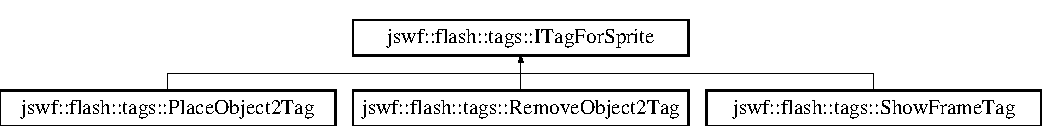
\includegraphics[height=1.696970cm]{classjswf_1_1flash_1_1tags_1_1_i_tag_for_sprite}
\end{center}
\end{figure}
\subsection*{Public Member Functions}
\begin{DoxyCompactItemize}
\item 
\hypertarget{classjswf_1_1flash_1_1tags_1_1_i_tag_for_sprite_a335f90384979e16cf1459de8168d929f}{virtual void {\bfseries apply\+To\+Sprite} (\hyperlink{classjswf_1_1flash_1_1_sprite}{Sprite} \&sprite)=0}\label{classjswf_1_1flash_1_1tags_1_1_i_tag_for_sprite_a335f90384979e16cf1459de8168d929f}

\end{DoxyCompactItemize}


\subsection{Detailed Description}
Interface for {\ttfamily T\+A\+G}s that implement actions to be performed on instances of \hyperlink{classjswf_1_1flash_1_1_sprite}{Sprite}. 

The documentation for this class was generated from the following file\+:\begin{DoxyCompactItemize}
\item 
jswf/flash/tags/\hyperlink{_i_tag_for_sprite_8h}{I\+Tag\+For\+Sprite.\+h}\end{DoxyCompactItemize}

\hypertarget{classjswf_1_1flash_1_1styles_1_1_line_style}{\section{jswf\+:\+:flash\+:\+:styles\+:\+:Line\+Style Class Reference}
\label{classjswf_1_1flash_1_1styles_1_1_line_style}\index{jswf\+::flash\+::styles\+::\+Line\+Style@{jswf\+::flash\+::styles\+::\+Line\+Style}}
}
\subsection*{Public Attributes}
\begin{DoxyCompactItemize}
\item 
\hypertarget{classjswf_1_1flash_1_1styles_1_1_line_style_a4812ec865db585131d277d959aed49d3}{uint32\+\_\+t {\bfseries id}}\label{classjswf_1_1flash_1_1styles_1_1_line_style_a4812ec865db585131d277d959aed49d3}

\item 
\hypertarget{classjswf_1_1flash_1_1styles_1_1_line_style_ae981bc9ccf17f98db10ced8846fed022}{uint16\+\_\+t {\bfseries width}}\label{classjswf_1_1flash_1_1styles_1_1_line_style_ae981bc9ccf17f98db10ced8846fed022}

\item 
\hypertarget{classjswf_1_1flash_1_1styles_1_1_line_style_ae4ec4dd5acb2e8730817ac443c76c2ad}{\hyperlink{structjswf_1_1flash_1_1_r_g_b_a}{R\+G\+B\+A} {\bfseries color}}\label{classjswf_1_1flash_1_1styles_1_1_line_style_ae4ec4dd5acb2e8730817ac443c76c2ad}

\end{DoxyCompactItemize}


The documentation for this class was generated from the following file\+:\begin{DoxyCompactItemize}
\item 
jswf/flash/styles/Line\+Style.\+h\end{DoxyCompactItemize}

\hypertarget{classjswf_1_1avm2_1_1ast_1_1_local_node}{\section{jswf\+:\+:avm2\+:\+:ast\+:\+:Local\+Node Class Reference}
\label{classjswf_1_1avm2_1_1ast_1_1_local_node}\index{jswf\+::avm2\+::ast\+::\+Local\+Node@{jswf\+::avm2\+::ast\+::\+Local\+Node}}
}


Describes a local register ({\ttfamily this}, arguments and local variables).  




{\ttfamily \#include $<$Node.\+h$>$}

Inheritance diagram for jswf\+:\+:avm2\+:\+:ast\+:\+:Local\+Node\+:\begin{figure}[H]
\begin{center}
\leavevmode
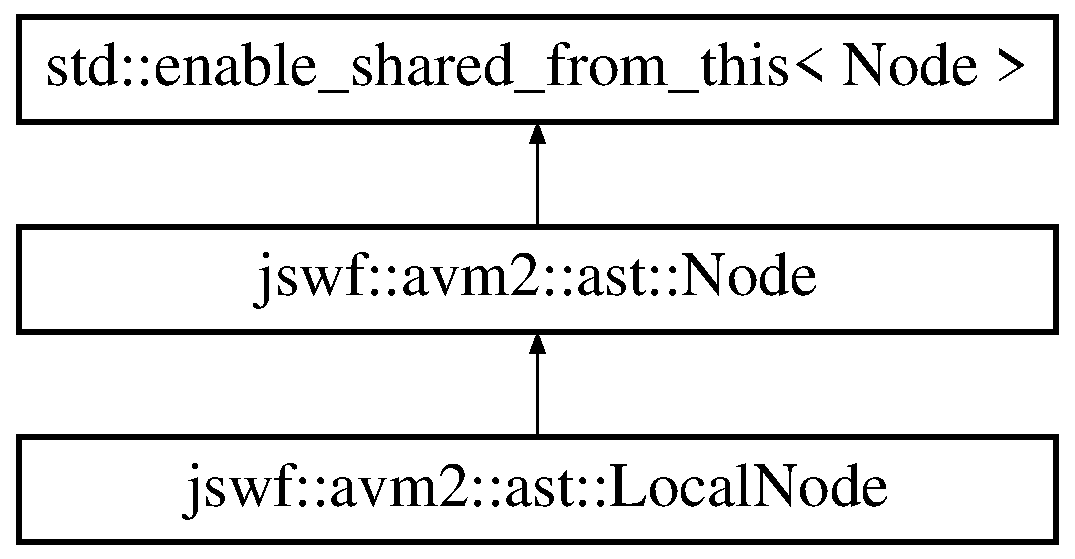
\includegraphics[height=3.000000cm]{classjswf_1_1avm2_1_1ast_1_1_local_node}
\end{center}
\end{figure}
\subsection*{Public Member Functions}
\begin{DoxyCompactItemize}
\item 
\hypertarget{classjswf_1_1avm2_1_1ast_1_1_local_node_ab99bfb86b8bf0ac14ea885643c2374c6}{{\bfseries Local\+Node} (\hyperlink{namespacejswf_aa10d9ddca2a6a5debdc261dfae3d1117}{u30\+\_\+t} index, \hyperlink{structjswf_1_1avm2_1_1_method_info}{Method\+Info} \&info)}\label{classjswf_1_1avm2_1_1ast_1_1_local_node_ab99bfb86b8bf0ac14ea885643c2374c6}

\item 
\hypertarget{classjswf_1_1avm2_1_1ast_1_1_local_node_a623638809696bad0f4a5142a85064b96}{virtual std\+::string {\bfseries to\+String} ()}\label{classjswf_1_1avm2_1_1ast_1_1_local_node_a623638809696bad0f4a5142a85064b96}

\end{DoxyCompactItemize}
\subsection*{Public Attributes}
\begin{DoxyCompactItemize}
\item 
\hypertarget{classjswf_1_1avm2_1_1ast_1_1_local_node_ab1dbfacd9a0bca73090105a142e0e687}{bool {\bfseries is\+Temporary} = false}\label{classjswf_1_1avm2_1_1ast_1_1_local_node_ab1dbfacd9a0bca73090105a142e0e687}

\item 
\hypertarget{classjswf_1_1avm2_1_1ast_1_1_local_node_a84dfe94d05763357c50d7058f6a002e0}{\hyperlink{namespacejswf_aa10d9ddca2a6a5debdc261dfae3d1117}{u30\+\_\+t} {\bfseries index}}\label{classjswf_1_1avm2_1_1ast_1_1_local_node_a84dfe94d05763357c50d7058f6a002e0}

\item 
\hypertarget{classjswf_1_1avm2_1_1ast_1_1_local_node_a9705e8cd202c70cf19db02f3ba5745d6}{std\+::string {\bfseries name}}\label{classjswf_1_1avm2_1_1ast_1_1_local_node_a9705e8cd202c70cf19db02f3ba5745d6}

\end{DoxyCompactItemize}


\subsection{Detailed Description}
Describes a local register ({\ttfamily this}, arguments and local variables). 

The documentation for this class was generated from the following file\+:\begin{DoxyCompactItemize}
\item 
jswf/avm2/ast/Node.\+h\end{DoxyCompactItemize}

\hypertarget{structjswf_1_1flash_1_1_matrix}{\section{jswf\+:\+:flash\+:\+:Matrix Struct Reference}
\label{structjswf_1_1flash_1_1_matrix}\index{jswf\+::flash\+::\+Matrix@{jswf\+::flash\+::\+Matrix}}
}


Represents {\ttfamily M\+A\+T\+R\+I\+X} records.  




{\ttfamily \#include $<$Structs.\+h$>$}

\subsection*{Public Member Functions}
\begin{DoxyCompactItemize}
\item 
void \hyperlink{structjswf_1_1flash_1_1_matrix_ae8dfa5d146be75927027d747d63cb327}{transform} (\hyperlink{namespacejswf_aa56b2b764590a9e19a5e66693364aceb}{sb\+\_\+t} \&x, \hyperlink{namespacejswf_aa56b2b764590a9e19a5e66693364aceb}{sb\+\_\+t} \&y) const 
\begin{DoxyCompactList}\small\item\em Transforms a point using this \hyperlink{structjswf_1_1flash_1_1_matrix}{Matrix}. \end{DoxyCompactList}\item 
bool \hyperlink{structjswf_1_1flash_1_1_matrix_adbd0725baff1dff4b83f8ee959c0ea73}{inverse} (\hyperlink{structjswf_1_1flash_1_1_matrix}{Matrix} \&result) const 
\begin{DoxyCompactList}\small\item\em Calculates the inverse of this \hyperlink{structjswf_1_1flash_1_1_matrix}{Matrix}. \end{DoxyCompactList}\end{DoxyCompactItemize}
\subsection*{Static Public Member Functions}
\begin{DoxyCompactItemize}
\item 
static void \hyperlink{structjswf_1_1flash_1_1_matrix_a29e96996ccb5f7dba395bfda3c0aa45a}{product} (\hyperlink{structjswf_1_1flash_1_1_matrix}{Matrix} \&result, const \hyperlink{structjswf_1_1flash_1_1_matrix}{Matrix} \&a, const \hyperlink{structjswf_1_1flash_1_1_matrix}{Matrix} \&b)
\begin{DoxyCompactList}\small\item\em Calculates the product of two instances of \hyperlink{structjswf_1_1flash_1_1_matrix}{Matrix}. \end{DoxyCompactList}\end{DoxyCompactItemize}
\subsection*{Public Attributes}
\begin{DoxyCompactItemize}
\item 
\hypertarget{structjswf_1_1flash_1_1_matrix_a9cd4ef0a19f1559a57e777790ff1b22c}{\hyperlink{namespacejswf_a419cb8aa8b625074e6753d189783b2f4}{fb\+\_\+t} \hyperlink{structjswf_1_1flash_1_1_matrix_a9cd4ef0a19f1559a57e777790ff1b22c}{sx} = 1}\label{structjswf_1_1flash_1_1_matrix_a9cd4ef0a19f1559a57e777790ff1b22c}

\begin{DoxyCompactList}\small\item\em Scale of the x-\/coordinate. \end{DoxyCompactList}\item 
\hypertarget{structjswf_1_1flash_1_1_matrix_a96f5b9292d1354f1b87a950692aa328e}{\hyperlink{namespacejswf_a419cb8aa8b625074e6753d189783b2f4}{fb\+\_\+t} \hyperlink{structjswf_1_1flash_1_1_matrix_a96f5b9292d1354f1b87a950692aa328e}{sy} = 1}\label{structjswf_1_1flash_1_1_matrix_a96f5b9292d1354f1b87a950692aa328e}

\begin{DoxyCompactList}\small\item\em Scale of the y-\/coordinate. \end{DoxyCompactList}\item 
\hypertarget{structjswf_1_1flash_1_1_matrix_a23cb93894dfbdd1986815751c10edb2e}{\hyperlink{namespacejswf_a419cb8aa8b625074e6753d189783b2f4}{fb\+\_\+t} \hyperlink{structjswf_1_1flash_1_1_matrix_a23cb93894dfbdd1986815751c10edb2e}{r0} = 0}\label{structjswf_1_1flash_1_1_matrix_a23cb93894dfbdd1986815751c10edb2e}

\begin{DoxyCompactList}\small\item\em Rotation-\/skew (y =$>$ x') \end{DoxyCompactList}\item 
\hypertarget{structjswf_1_1flash_1_1_matrix_aa641e22c17d8ffc429975889c440eb7a}{\hyperlink{namespacejswf_a419cb8aa8b625074e6753d189783b2f4}{fb\+\_\+t} \hyperlink{structjswf_1_1flash_1_1_matrix_aa641e22c17d8ffc429975889c440eb7a}{r1} = 0}\label{structjswf_1_1flash_1_1_matrix_aa641e22c17d8ffc429975889c440eb7a}

\begin{DoxyCompactList}\small\item\em Rotation-\/skew (x =$>$ y') \end{DoxyCompactList}\item 
\hypertarget{structjswf_1_1flash_1_1_matrix_aafcf9abe180ac3e6097b9b030709f2eb}{\hyperlink{namespacejswf_aa56b2b764590a9e19a5e66693364aceb}{sb\+\_\+t} \hyperlink{structjswf_1_1flash_1_1_matrix_aafcf9abe180ac3e6097b9b030709f2eb}{tx} = 0}\label{structjswf_1_1flash_1_1_matrix_aafcf9abe180ac3e6097b9b030709f2eb}

\begin{DoxyCompactList}\small\item\em Translation of the x-\/coordinate. \end{DoxyCompactList}\item 
\hypertarget{structjswf_1_1flash_1_1_matrix_acec2419f445aa5a0e5a39ab321ad8805}{\hyperlink{namespacejswf_aa56b2b764590a9e19a5e66693364aceb}{sb\+\_\+t} \hyperlink{structjswf_1_1flash_1_1_matrix_acec2419f445aa5a0e5a39ab321ad8805}{ty} = 0}\label{structjswf_1_1flash_1_1_matrix_acec2419f445aa5a0e5a39ab321ad8805}

\begin{DoxyCompactList}\small\item\em Translation of the y-\/coordinate. \end{DoxyCompactList}\end{DoxyCompactItemize}


\subsection{Detailed Description}
Represents {\ttfamily M\+A\+T\+R\+I\+X} records. 

\[ \begin{bmatrix} s_x & r_1 & t_x \\ r_0 & s_y & t_y \\ 0 & 0 & 1 \end{bmatrix} \] \begin{DoxyRefDesc}{Todo}
\item[\hyperlink{todo__todo000013}{Todo}]These structures are in the wrong file. \end{DoxyRefDesc}


\subsection{Member Function Documentation}
\hypertarget{structjswf_1_1flash_1_1_matrix_adbd0725baff1dff4b83f8ee959c0ea73}{\index{jswf\+::flash\+::\+Matrix@{jswf\+::flash\+::\+Matrix}!inverse@{inverse}}
\index{inverse@{inverse}!jswf\+::flash\+::\+Matrix@{jswf\+::flash\+::\+Matrix}}
\subsubsection[{inverse}]{\setlength{\rightskip}{0pt plus 5cm}bool jswf\+::flash\+::\+Matrix\+::inverse (
\begin{DoxyParamCaption}
\item[{{\bf Matrix} \&}]{result}
\end{DoxyParamCaption}
) const\hspace{0.3cm}{\ttfamily [inline]}}}\label{structjswf_1_1flash_1_1_matrix_adbd0725baff1dff4b83f8ee959c0ea73}


Calculates the inverse of this \hyperlink{structjswf_1_1flash_1_1_matrix}{Matrix}. 

\[ \begin{bmatrix} s_x & r_1 & t_x \\ r_0 & s_y & t_y \\ 0 & 0 & 1 \end{bmatrix}^{-1} = \frac{1}{s_x s_y - r_0 r_1} \begin{bmatrix} s_y & -r_1 & t_y r_1 - t_x s_y \\ -r_0 & s_x & t_x r_0 - t_y s_x \\ 0 & 0 & 1 \end{bmatrix} \] 
\begin{DoxyParams}[1]{Parameters}
\mbox{\tt out}  & {\em result} & A reference to the \hyperlink{structjswf_1_1flash_1_1_matrix}{Matrix} to store the result in. \\
\hline
\end{DoxyParams}
\begin{DoxyReturn}{Returns}
{\ttfamily true} if the operation was successful, {\ttfamily false} if the \hyperlink{structjswf_1_1flash_1_1_matrix}{Matrix} cannot be inversed 
\end{DoxyReturn}
\begin{DoxyWarning}{Warning}
This will fail if the determinant of this \hyperlink{structjswf_1_1flash_1_1_matrix}{Matrix} ( $s_x s_y - r_0 r_1$) equals zero. In that case the given \hyperlink{structjswf_1_1flash_1_1_matrix}{Matrix} cannot be inversed and no write to result occurs. 
\end{DoxyWarning}
\hypertarget{structjswf_1_1flash_1_1_matrix_a29e96996ccb5f7dba395bfda3c0aa45a}{\index{jswf\+::flash\+::\+Matrix@{jswf\+::flash\+::\+Matrix}!product@{product}}
\index{product@{product}!jswf\+::flash\+::\+Matrix@{jswf\+::flash\+::\+Matrix}}
\subsubsection[{product}]{\setlength{\rightskip}{0pt plus 5cm}static void jswf\+::flash\+::\+Matrix\+::product (
\begin{DoxyParamCaption}
\item[{{\bf Matrix} \&}]{result, }
\item[{const {\bf Matrix} \&}]{a, }
\item[{const {\bf Matrix} \&}]{b}
\end{DoxyParamCaption}
)\hspace{0.3cm}{\ttfamily [inline]}, {\ttfamily [static]}}}\label{structjswf_1_1flash_1_1_matrix_a29e96996ccb5f7dba395bfda3c0aa45a}


Calculates the product of two instances of \hyperlink{structjswf_1_1flash_1_1_matrix}{Matrix}. 

given $a, b, c \in \mathbb{R}^{3 \times 3}$~\newline
 \[a \left( b \begin{pmatrix}x\\y\\1\end{pmatrix} \right) = c \begin{pmatrix}x\\y\\1\end{pmatrix}\]~\newline
 \[ c = a \times b = \begin{bmatrix} s_{x_a}s_{x_b} + r_{1_a}r_{0_b} & s_{x_a}r_{1_b} + r_{1_a}s_{y_b} & s_{x_a}t_{x_b} + r_{1_a}t_{y_b} + t_{x_a} \\ s_{y_a}r_{0_b} + r_{0_a}s_{x_b} & s_{y_a}s_{y_b} + r_{0_a}r_{1_b} & s_{y_a}t_{y_b} + r_{0_a}t_{x_b} + t_{y_a} \\ 0 & 0 & 1 \end{bmatrix} \] 
\begin{DoxyParams}[1]{Parameters}
\mbox{\tt out}  & {\em result} & A reference to the \hyperlink{structjswf_1_1flash_1_1_matrix}{Matrix} to store the result in. \\
\hline
\mbox{\tt in}  & {\em a,b} & The operands. \\
\hline
\end{DoxyParams}
\hypertarget{structjswf_1_1flash_1_1_matrix_ae8dfa5d146be75927027d747d63cb327}{\index{jswf\+::flash\+::\+Matrix@{jswf\+::flash\+::\+Matrix}!transform@{transform}}
\index{transform@{transform}!jswf\+::flash\+::\+Matrix@{jswf\+::flash\+::\+Matrix}}
\subsubsection[{transform}]{\setlength{\rightskip}{0pt plus 5cm}void jswf\+::flash\+::\+Matrix\+::transform (
\begin{DoxyParamCaption}
\item[{{\bf sb\+\_\+t} \&}]{x, }
\item[{{\bf sb\+\_\+t} \&}]{y}
\end{DoxyParamCaption}
) const\hspace{0.3cm}{\ttfamily [inline]}}}\label{structjswf_1_1flash_1_1_matrix_ae8dfa5d146be75927027d747d63cb327}


Transforms a point using this \hyperlink{structjswf_1_1flash_1_1_matrix}{Matrix}. 

\[ \begin{bmatrix} s_x & r_1 & t_x \\ r_0 & s_y & t_y \\ 0 & 0 & 1 \end{bmatrix} \begin{pmatrix}x\\y\\1\end{pmatrix} = \begin{pmatrix} x \cdot s_x + y \cdot r_1 + t_x \\ y \cdot s_y + x \cdot r_0 + t_y \\ 1 \end{pmatrix} \] 

The documentation for this struct was generated from the following file\+:\begin{DoxyCompactItemize}
\item 
jswf/flash/\hyperlink{_structs_8h}{Structs.\+h}\end{DoxyCompactItemize}

\hypertarget{structjswf_1_1avm2_1_1_metadata}{\section{jswf\+:\+:avm2\+:\+:Metadata Struct Reference}
\label{structjswf_1_1avm2_1_1_metadata}\index{jswf\+::avm2\+::\+Metadata@{jswf\+::avm2\+::\+Metadata}}
}
\subsection*{Public Attributes}
\begin{DoxyCompactItemize}
\item 
\hypertarget{structjswf_1_1avm2_1_1_metadata_ab20e450b84501dad71897274067ea3b3}{std\+::string $\ast$ {\bfseries name}}\label{structjswf_1_1avm2_1_1_metadata_ab20e450b84501dad71897274067ea3b3}

\item 
\hypertarget{structjswf_1_1avm2_1_1_metadata_a7de8e78cb0a42a1e83939d62b074df72}{std\+::vector$<$ \hyperlink{structjswf_1_1avm2_1_1_metadata_item}{Metadata\+Item} $>$ {\bfseries items}}\label{structjswf_1_1avm2_1_1_metadata_a7de8e78cb0a42a1e83939d62b074df72}

\end{DoxyCompactItemize}


The documentation for this struct was generated from the following file\+:\begin{DoxyCompactItemize}
\item 
jswf/avm2/Metadata.\+h\end{DoxyCompactItemize}

\hypertarget{structjswf_1_1avm2_1_1_metadata_item}{\section{jswf\+:\+:avm2\+:\+:Metadata\+Item Struct Reference}
\label{structjswf_1_1avm2_1_1_metadata_item}\index{jswf\+::avm2\+::\+Metadata\+Item@{jswf\+::avm2\+::\+Metadata\+Item}}
}
\subsection*{Public Attributes}
\begin{DoxyCompactItemize}
\item 
\hypertarget{structjswf_1_1avm2_1_1_metadata_item_a82d0ded36df062564eda6a6792d1706f}{std\+::string $\ast$ {\bfseries key}}\label{structjswf_1_1avm2_1_1_metadata_item_a82d0ded36df062564eda6a6792d1706f}

\item 
\hypertarget{structjswf_1_1avm2_1_1_metadata_item_ad9a45b5a286778db5701cfb9c0333a07}{std\+::string $\ast$ {\bfseries value}}\label{structjswf_1_1avm2_1_1_metadata_item_ad9a45b5a286778db5701cfb9c0333a07}

\end{DoxyCompactItemize}


The documentation for this struct was generated from the following file\+:\begin{DoxyCompactItemize}
\item 
jswf/avm2/Metadata.\+h\end{DoxyCompactItemize}

\hypertarget{structjswf_1_1avm2_1_1_method_body}{\section{jswf\+:\+:avm2\+:\+:Method\+Body Struct Reference}
\label{structjswf_1_1avm2_1_1_method_body}\index{jswf\+::avm2\+::\+Method\+Body@{jswf\+::avm2\+::\+Method\+Body}}
}
\subsection*{Public Attributes}
\begin{DoxyCompactItemize}
\item 
\hypertarget{structjswf_1_1avm2_1_1_method_body_a910d1f7ef990dc830fc1b91416e13596}{\hyperlink{structjswf_1_1avm2_1_1_method_info}{Method\+Info} $\ast$ {\bfseries method}}\label{structjswf_1_1avm2_1_1_method_body_a910d1f7ef990dc830fc1b91416e13596}

\item 
\hypertarget{structjswf_1_1avm2_1_1_method_body_a94d21bb9993138bfd197c2b6e74af4ac}{\hyperlink{namespacejswf_aa10d9ddca2a6a5debdc261dfae3d1117}{u30\+\_\+t} {\bfseries max\+Stack}}\label{structjswf_1_1avm2_1_1_method_body_a94d21bb9993138bfd197c2b6e74af4ac}

\item 
\hypertarget{structjswf_1_1avm2_1_1_method_body_ae0689c37a9c87bd4fb6054781e524384}{\hyperlink{namespacejswf_aa10d9ddca2a6a5debdc261dfae3d1117}{u30\+\_\+t} {\bfseries local\+Count}}\label{structjswf_1_1avm2_1_1_method_body_ae0689c37a9c87bd4fb6054781e524384}

\item 
\hypertarget{structjswf_1_1avm2_1_1_method_body_aa5589f5ddd2873563fa7b50a5ce71ab0}{\hyperlink{namespacejswf_aa10d9ddca2a6a5debdc261dfae3d1117}{u30\+\_\+t} {\bfseries init\+Scope\+Depth}}\label{structjswf_1_1avm2_1_1_method_body_aa5589f5ddd2873563fa7b50a5ce71ab0}

\item 
\hypertarget{structjswf_1_1avm2_1_1_method_body_a3ab78ba183a94a5fea22bbfebb78d0f7}{\hyperlink{namespacejswf_aa10d9ddca2a6a5debdc261dfae3d1117}{u30\+\_\+t} {\bfseries max\+Scope\+Depth}}\label{structjswf_1_1avm2_1_1_method_body_a3ab78ba183a94a5fea22bbfebb78d0f7}

\item 
\hypertarget{structjswf_1_1avm2_1_1_method_body_a61b6d8ef01100debc05786be059d8f21}{\hyperlink{namespacejswf_a755127d61081aa8af105eb800aa2c1ec}{string} {\bfseries code}}\label{structjswf_1_1avm2_1_1_method_body_a61b6d8ef01100debc05786be059d8f21}

\item 
\hypertarget{structjswf_1_1avm2_1_1_method_body_a6550b0bdc8c27fb534d263b832ac265a}{std\+::vector$<$ \hyperlink{structjswf_1_1avm2_1_1_exception_info}{Exception\+Info} $>$ {\bfseries exceptions}}\label{structjswf_1_1avm2_1_1_method_body_a6550b0bdc8c27fb534d263b832ac265a}

\item 
\hypertarget{structjswf_1_1avm2_1_1_method_body_ae328107b045423b2024881158c8d3d92}{std\+::vector$<$ std\+::shared\+\_\+ptr\\*
$<$ \hyperlink{structjswf_1_1avm2_1_1_trait_info}{Trait\+Info} $>$ $>$ {\bfseries traits}}\label{structjswf_1_1avm2_1_1_method_body_ae328107b045423b2024881158c8d3d92}

\end{DoxyCompactItemize}


The documentation for this struct was generated from the following file\+:\begin{DoxyCompactItemize}
\item 
jswf/avm2/Method\+Info.\+h\end{DoxyCompactItemize}

\hypertarget{structjswf_1_1avm2_1_1_method_info}{\section{jswf\+:\+:avm2\+:\+:Method\+Info Struct Reference}
\label{structjswf_1_1avm2_1_1_method_info}\index{jswf\+::avm2\+::\+Method\+Info@{jswf\+::avm2\+::\+Method\+Info}}
}
\subsection*{Public Types}
\begin{DoxyCompactItemize}
\item 
\hypertarget{structjswf_1_1avm2_1_1_method_info_a98d7a90e5579ad8d853f442fadbada70}{enum {\bfseries Flags} \+: u8\+\_\+t \{ \\*
{\bfseries Needs\+Arguments\+Flag} = 0x01, 
{\bfseries Needs\+Activation\+Flag} = 0x02, 
{\bfseries Needs\+Rest\+Flag} = 0x04, 
{\bfseries Has\+Optional\+Flag} = 0x08, 
\\*
{\bfseries Set\+Dxns\+Flag} = 0x40, 
{\bfseries Has\+Param\+Names\+Flag} = 0x80
 \}}\label{structjswf_1_1avm2_1_1_method_info_a98d7a90e5579ad8d853f442fadbada70}

\end{DoxyCompactItemize}
\subsection*{Public Attributes}
\begin{DoxyCompactItemize}
\item 
\hypertarget{structjswf_1_1avm2_1_1_method_info_aa917cf2cf9b382d303393a35582c26cd}{\hyperlink{namespacejswf_aa10d9ddca2a6a5debdc261dfae3d1117}{u30\+\_\+t} {\bfseries param\+Count}}\label{structjswf_1_1avm2_1_1_method_info_aa917cf2cf9b382d303393a35582c26cd}

\item 
\hypertarget{structjswf_1_1avm2_1_1_method_info_abed1dca0105db41c12af0134126b67d0}{Multiname\+Ptr {\bfseries return\+Type}}\label{structjswf_1_1avm2_1_1_method_info_abed1dca0105db41c12af0134126b67d0}

\item 
\hypertarget{structjswf_1_1avm2_1_1_method_info_a2559fe56e7ad0b0ef520087d39903402}{std\+::vector$<$ Multiname\+Ptr $>$ {\bfseries param\+Types}}\label{structjswf_1_1avm2_1_1_method_info_a2559fe56e7ad0b0ef520087d39903402}

\item 
\hypertarget{structjswf_1_1avm2_1_1_method_info_a655d4695c78620babaaca2940206874e}{\hyperlink{namespacejswf_a755127d61081aa8af105eb800aa2c1ec}{string} $\ast$ {\bfseries name}}\label{structjswf_1_1avm2_1_1_method_info_a655d4695c78620babaaca2940206874e}

\item 
\hypertarget{structjswf_1_1avm2_1_1_method_info_a5f3d480bd81550cd72c9254fa73dc9b2}{Flags {\bfseries flags}}\label{structjswf_1_1avm2_1_1_method_info_a5f3d480bd81550cd72c9254fa73dc9b2}

\item 
\hypertarget{structjswf_1_1avm2_1_1_method_info_ab87f16ec0fd2fcfd4c4f871c9f9641d0}{std\+::vector$<$ \hyperlink{structjswf_1_1avm2_1_1_option_detail}{Option\+Detail} $>$ {\bfseries options}}\label{structjswf_1_1avm2_1_1_method_info_ab87f16ec0fd2fcfd4c4f871c9f9641d0}

\item 
\hypertarget{structjswf_1_1avm2_1_1_method_info_a1bbb310593650d6d0312a790c09cb61a}{std\+::vector$<$ \hyperlink{namespacejswf_a755127d61081aa8af105eb800aa2c1ec}{string} $\ast$ $>$ {\bfseries param\+Names}}\label{structjswf_1_1avm2_1_1_method_info_a1bbb310593650d6d0312a790c09cb61a}

\item 
\hypertarget{structjswf_1_1avm2_1_1_method_info_a3b9b530afa4a78fb463669c0a4aa454e}{\hyperlink{structjswf_1_1avm2_1_1_method_body}{Method\+Body} $\ast$ {\bfseries body} = N\+U\+L\+L}\label{structjswf_1_1avm2_1_1_method_info_a3b9b530afa4a78fb463669c0a4aa454e}

\item 
\hypertarget{structjswf_1_1avm2_1_1_method_info_a759661b09d28773bf6868fad09e0318f}{builtin\+\_\+method\+\_\+t $\ast$ {\bfseries native\+Impl} = N\+U\+L\+L}\label{structjswf_1_1avm2_1_1_method_info_a759661b09d28773bf6868fad09e0318f}

\item 
\hypertarget{structjswf_1_1avm2_1_1_method_info_aebf942b78b514c00f0343a28b1786035}{\hyperlink{classjswf_1_1avm2_1_1_a_b_c_file}{A\+B\+C\+File} $\ast$ {\bfseries file}}\label{structjswf_1_1avm2_1_1_method_info_aebf942b78b514c00f0343a28b1786035}

\end{DoxyCompactItemize}


The documentation for this struct was generated from the following file\+:\begin{DoxyCompactItemize}
\item 
jswf/avm2/Method\+Info.\+h\end{DoxyCompactItemize}

\hypertarget{classjswf_1_1avm2_1_1_method_object}{\section{jswf\+:\+:avm2\+:\+:Method\+Object Class Reference}
\label{classjswf_1_1avm2_1_1_method_object}\index{jswf\+::avm2\+::\+Method\+Object@{jswf\+::avm2\+::\+Method\+Object}}
}


Represents a method that was created as a trait of an instance or a class.  




{\ttfamily \#include $<$Object.\+h$>$}

Inheritance diagram for jswf\+:\+:avm2\+:\+:Method\+Object\+:\begin{figure}[H]
\begin{center}
\leavevmode
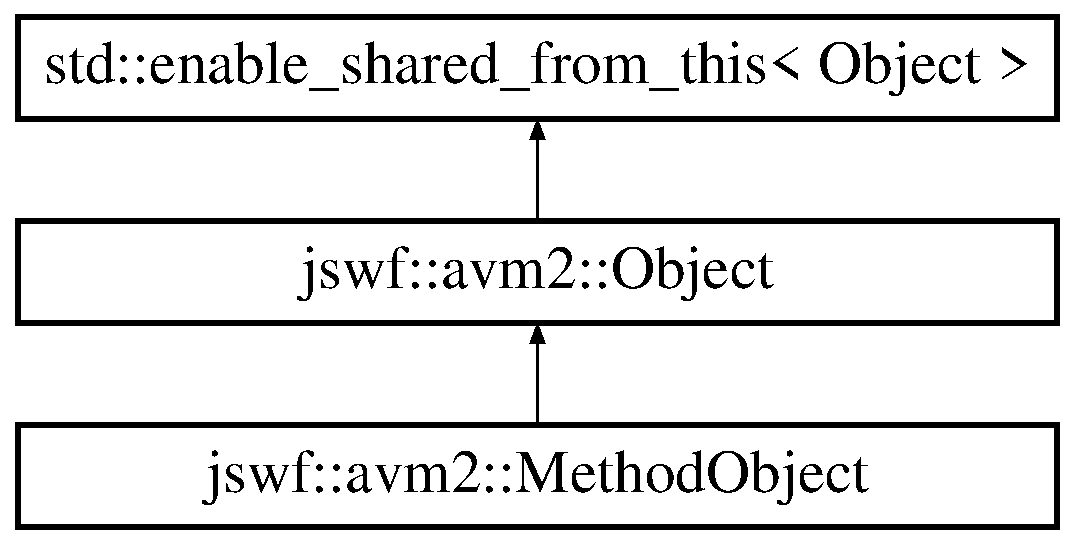
\includegraphics[height=3.000000cm]{classjswf_1_1avm2_1_1_method_object}
\end{center}
\end{figure}
\subsection*{Public Member Functions}
\begin{DoxyCompactItemize}
\item 
\hypertarget{classjswf_1_1avm2_1_1_method_object_aaed0d33e8acaa53786d16df44b97e8af}{{\bfseries Method\+Object} (\hyperlink{classjswf_1_1avm2_1_1_v_m}{V\+M} $\ast$vm, const Object\+Ptr \&recv, \hyperlink{structjswf_1_1avm2_1_1_method_info}{Method\+Info} $\ast$value)}\label{classjswf_1_1avm2_1_1_method_object_aaed0d33e8acaa53786d16df44b97e8af}

\item 
std\+::string \hyperlink{classjswf_1_1avm2_1_1_method_object_a166c823f400cdc125e21794f31d25d3d}{coerce\+\_\+s} () const 
\begin{DoxyCompactList}\small\item\em Converts to {\ttfamily std\+::string} (E\+C\+M\+A-\/262, section 9.\+8 {\itshape To\+String}) \end{DoxyCompactList}\item 
\hypertarget{classjswf_1_1avm2_1_1_method_object_ab4985a2c40310dca67ad070ab9b3aefa}{Object\+Ptr {\bfseries ecma\+Call} (\hyperlink{classjswf_1_1avm2_1_1_v_m}{V\+M} \&vm, std\+::vector$<$ Object\+Ptr $>$ \&args) const }\label{classjswf_1_1avm2_1_1_method_object_ab4985a2c40310dca67ad070ab9b3aefa}

\end{DoxyCompactItemize}
\subsection*{Public Attributes}
\begin{DoxyCompactItemize}
\item 
\hypertarget{classjswf_1_1avm2_1_1_method_object_aaf875ea341bb147e53d4b66827d9b0be}{Object\+Ptr {\bfseries receiver}}\label{classjswf_1_1avm2_1_1_method_object_aaf875ea341bb147e53d4b66827d9b0be}

\item 
\hypertarget{classjswf_1_1avm2_1_1_method_object_acf598d163383a3aa2bff25e93fb0dfd9}{\hyperlink{structjswf_1_1avm2_1_1_method_info}{Method\+Info} $\ast$ {\bfseries value}}\label{classjswf_1_1avm2_1_1_method_object_acf598d163383a3aa2bff25e93fb0dfd9}

\end{DoxyCompactItemize}
\subsection*{Additional Inherited Members}


\subsection{Detailed Description}
Represents a method that was created as a trait of an instance or a class. 

Note that executing {\ttfamily \mbox{[}\mbox{[}Call\mbox{]}\mbox{]}} on a \hyperlink{classjswf_1_1avm2_1_1_method_object}{Method\+Object} will always override the implicit (receiver) argument. 

\subsection{Member Function Documentation}
\hypertarget{classjswf_1_1avm2_1_1_method_object_a166c823f400cdc125e21794f31d25d3d}{\index{jswf\+::avm2\+::\+Method\+Object@{jswf\+::avm2\+::\+Method\+Object}!coerce\+\_\+s@{coerce\+\_\+s}}
\index{coerce\+\_\+s@{coerce\+\_\+s}!jswf\+::avm2\+::\+Method\+Object@{jswf\+::avm2\+::\+Method\+Object}}
\subsubsection[{coerce\+\_\+s}]{\setlength{\rightskip}{0pt plus 5cm}std\+::string jswf\+::avm2\+::\+Method\+Object\+::coerce\+\_\+s (
\begin{DoxyParamCaption}
{}
\end{DoxyParamCaption}
) const\hspace{0.3cm}{\ttfamily [inline]}, {\ttfamily [virtual]}}}\label{classjswf_1_1avm2_1_1_method_object_a166c823f400cdc125e21794f31d25d3d}


Converts to {\ttfamily std\+::string} (E\+C\+M\+A-\/262, section 9.\+8 {\itshape To\+String}) 

\begin{DoxyRefDesc}{Todo}
\item[\hyperlink{todo__todo000007}{Todo}]Implement 9.\+8.\+1 \end{DoxyRefDesc}


Reimplemented from \hyperlink{classjswf_1_1avm2_1_1_object_a69b39776062acaccd2cd2b5a1f937c9d}{jswf\+::avm2\+::\+Object}.



The documentation for this class was generated from the following files\+:\begin{DoxyCompactItemize}
\item 
jswf/avm2/Object.\+h\item 
jswf/avm2/Object.\+cpp\end{DoxyCompactItemize}

\hypertarget{structjswf_1_1avm2_1_1_method_trait_info}{\section{jswf\+:\+:avm2\+:\+:Method\+Trait\+Info Struct Reference}
\label{structjswf_1_1avm2_1_1_method_trait_info}\index{jswf\+::avm2\+::\+Method\+Trait\+Info@{jswf\+::avm2\+::\+Method\+Trait\+Info}}
}
Inheritance diagram for jswf\+:\+:avm2\+:\+:Method\+Trait\+Info\+:\begin{figure}[H]
\begin{center}
\leavevmode
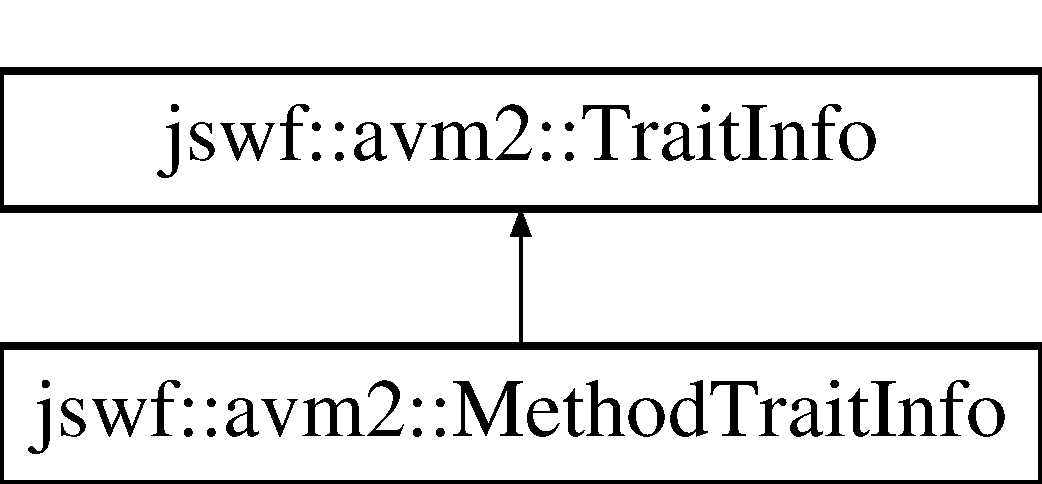
\includegraphics[height=2.000000cm]{structjswf_1_1avm2_1_1_method_trait_info}
\end{center}
\end{figure}
\subsection*{Public Attributes}
\begin{DoxyCompactItemize}
\item 
\hypertarget{structjswf_1_1avm2_1_1_method_trait_info_a965cbb880396d3ce1040962a0de7ab91}{\hyperlink{namespacejswf_aa10d9ddca2a6a5debdc261dfae3d1117}{u30\+\_\+t} {\bfseries disp\+Id}}\label{structjswf_1_1avm2_1_1_method_trait_info_a965cbb880396d3ce1040962a0de7ab91}

\item 
\hypertarget{structjswf_1_1avm2_1_1_method_trait_info_a4fb0b7ba917a0fc7c87c20b17f0b5ce0}{\hyperlink{structjswf_1_1avm2_1_1_method_info}{Method\+Info} $\ast$ {\bfseries method\+Info}}\label{structjswf_1_1avm2_1_1_method_trait_info_a4fb0b7ba917a0fc7c87c20b17f0b5ce0}

\end{DoxyCompactItemize}
\subsection*{Additional Inherited Members}


The documentation for this struct was generated from the following file\+:\begin{DoxyCompactItemize}
\item 
jswf/avm2/Trait\+Info.\+h\end{DoxyCompactItemize}

\hypertarget{classjswf_1_1avm2_1_1ast_1_1_monadic_node}{\section{jswf\+:\+:avm2\+:\+:ast\+:\+:Monadic\+Node Class Reference}
\label{classjswf_1_1avm2_1_1ast_1_1_monadic_node}\index{jswf\+::avm2\+::ast\+::\+Monadic\+Node@{jswf\+::avm2\+::ast\+::\+Monadic\+Node}}
}


Describes a monadic operation.  




{\ttfamily \#include $<$Node.\+h$>$}

Inheritance diagram for jswf\+:\+:avm2\+:\+:ast\+:\+:Monadic\+Node\+:\begin{figure}[H]
\begin{center}
\leavevmode
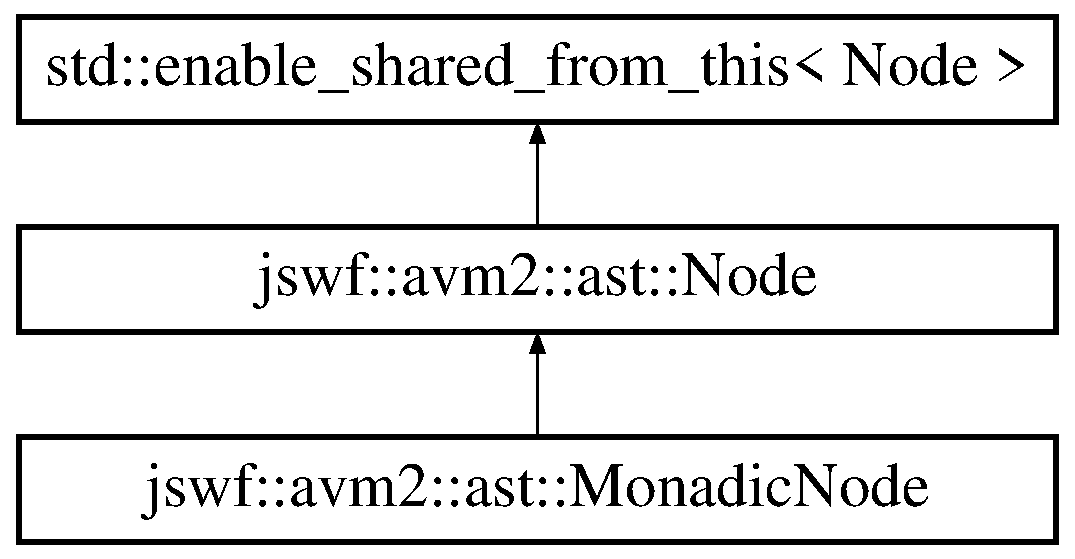
\includegraphics[height=3.000000cm]{classjswf_1_1avm2_1_1ast_1_1_monadic_node}
\end{center}
\end{figure}
\subsection*{Public Member Functions}
\begin{DoxyCompactItemize}
\item 
\hypertarget{classjswf_1_1avm2_1_1ast_1_1_monadic_node_a72474fdb0c21ed77e2134e26ed2fff22}{{\bfseries Monadic\+Node} (Node\+Ptr operand, std\+::string op, int p)}\label{classjswf_1_1avm2_1_1ast_1_1_monadic_node_a72474fdb0c21ed77e2134e26ed2fff22}

\item 
\hypertarget{classjswf_1_1avm2_1_1ast_1_1_monadic_node_a4070dd2e2c26f4022c9b763dade66ad7}{virtual std\+::string {\bfseries to\+String} ()}\label{classjswf_1_1avm2_1_1ast_1_1_monadic_node_a4070dd2e2c26f4022c9b763dade66ad7}

\end{DoxyCompactItemize}
\subsection*{Public Attributes}
\begin{DoxyCompactItemize}
\item 
\hypertarget{classjswf_1_1avm2_1_1ast_1_1_monadic_node_a84607e3fad013a6ae3fb62a6a3b773e0}{Node\+Ptr {\bfseries operand}}\label{classjswf_1_1avm2_1_1ast_1_1_monadic_node_a84607e3fad013a6ae3fb62a6a3b773e0}

\item 
\hypertarget{classjswf_1_1avm2_1_1ast_1_1_monadic_node_a8ca50b8283f93bc87b06b0a2b945c4d5}{std\+::string {\bfseries op}}\label{classjswf_1_1avm2_1_1ast_1_1_monadic_node_a8ca50b8283f93bc87b06b0a2b945c4d5}

\end{DoxyCompactItemize}


\subsection{Detailed Description}
Describes a monadic operation. 

The documentation for this class was generated from the following file\+:\begin{DoxyCompactItemize}
\item 
jswf/avm2/ast/Node.\+h\end{DoxyCompactItemize}

\hypertarget{structjswf_1_1avm2_1_1_multiname}{\section{jswf\+:\+:avm2\+:\+:Multiname Struct Reference}
\label{structjswf_1_1avm2_1_1_multiname}\index{jswf\+::avm2\+::\+Multiname@{jswf\+::avm2\+::\+Multiname}}
}
\subsection*{Public Types}
\begin{DoxyCompactItemize}
\item 
\hypertarget{structjswf_1_1avm2_1_1_multiname_ada7cf4bc0db7a67fd9ac73965ae3d7b9}{enum {\bfseries Kind} \+: u8\+\_\+t \{ \\*
{\bfseries Q\+Name\+Kind} = 0x07, 
{\bfseries Q\+Name\+A\+Kind} = 0x0\+D, 
{\bfseries R\+T\+Q\+Name\+Kind} = 0x0\+F, 
{\bfseries R\+T\+Q\+Name\+A\+Kind} = 0x10, 
\\*
{\bfseries R\+T\+Q\+Name\+L\+Kind} = 0x11, 
{\bfseries R\+T\+Q\+Name\+L\+A\+Kind} = 0x12, 
{\bfseries Multiname\+Kind} = 0x09, 
{\bfseries Multiname\+A\+Kind} = 0x0\+E, 
\\*
{\bfseries Multiname\+L\+Kind} = 0x1\+B, 
{\bfseries Multiname\+L\+A\+Kind} = 0x1\+C, 
{\bfseries Invalid\+Kind} = 0
 \}}\label{structjswf_1_1avm2_1_1_multiname_ada7cf4bc0db7a67fd9ac73965ae3d7b9}

\end{DoxyCompactItemize}
\subsection*{Public Member Functions}
\begin{DoxyCompactItemize}
\item 
\hypertarget{structjswf_1_1avm2_1_1_multiname_adaff16969a61aee2a61d94e190be2abb}{{\bfseries Multiname} (Kind kind)}\label{structjswf_1_1avm2_1_1_multiname_adaff16969a61aee2a61d94e190be2abb}

\item 
\hypertarget{structjswf_1_1avm2_1_1_multiname_a1c0b18cf3273f9c17974b3be94651f7d}{bool {\bfseries operator==} (const \hyperlink{structjswf_1_1avm2_1_1_multiname}{Multiname} \&rhs) const }\label{structjswf_1_1avm2_1_1_multiname_a1c0b18cf3273f9c17974b3be94651f7d}

\item 
\hypertarget{structjswf_1_1avm2_1_1_multiname_ad78ee0038f3ed1b83378b668c75e8e06}{void {\bfseries set\+Name} (std\+::string name)}\label{structjswf_1_1avm2_1_1_multiname_ad78ee0038f3ed1b83378b668c75e8e06}

\item 
\hypertarget{structjswf_1_1avm2_1_1_multiname_a8380725739ffd1ad4f00efac3f875de9}{void {\bfseries set\+N\+S} (Namespace\+Ptr ns)}\label{structjswf_1_1avm2_1_1_multiname_a8380725739ffd1ad4f00efac3f875de9}

\item 
\hypertarget{structjswf_1_1avm2_1_1_multiname_ae07c51d441478d22c20b9a53c429568e}{Kind {\bfseries get\+Kind} () const }\label{structjswf_1_1avm2_1_1_multiname_ae07c51d441478d22c20b9a53c429568e}

\item 
\hypertarget{structjswf_1_1avm2_1_1_multiname_aba782cb5a75fad2f3e0606e54480c3d3}{bool {\bfseries is\+Qualified} () const }\label{structjswf_1_1avm2_1_1_multiname_aba782cb5a75fad2f3e0606e54480c3d3}

\item 
\hypertarget{structjswf_1_1avm2_1_1_multiname_ac509d13e2fad07812d8e293888c85349}{std\+::string {\bfseries name\+String} () const }\label{structjswf_1_1avm2_1_1_multiname_ac509d13e2fad07812d8e293888c85349}

\end{DoxyCompactItemize}
\subsection*{Public Attributes}
\begin{DoxyCompactItemize}
\item 
\hypertarget{structjswf_1_1avm2_1_1_multiname_a7889ccdaa065487d132fea3483584d1c}{bool {\bfseries is\+Attribute}}\label{structjswf_1_1avm2_1_1_multiname_a7889ccdaa065487d132fea3483584d1c}

\item 
\hypertarget{structjswf_1_1avm2_1_1_multiname_a5899eff28deedf652d865aa2600525f5}{bool {\bfseries has\+Name}}\label{structjswf_1_1avm2_1_1_multiname_a5899eff28deedf652d865aa2600525f5}

\item 
\hypertarget{structjswf_1_1avm2_1_1_multiname_aa166b6549a3616cae069eb3de3d09a06}{bool {\bfseries has\+N\+S}}\label{structjswf_1_1avm2_1_1_multiname_aa166b6549a3616cae069eb3de3d09a06}

\item 
\hypertarget{structjswf_1_1avm2_1_1_multiname_a6c397704639dca3f1f17638e20b1a329}{bool {\bfseries has\+N\+S\+Set}}\label{structjswf_1_1avm2_1_1_multiname_a6c397704639dca3f1f17638e20b1a329}

\item 
\hypertarget{structjswf_1_1avm2_1_1_multiname_aa87f364be6754d915e3e3171e33c9943}{\hyperlink{namespacejswf_a755127d61081aa8af105eb800aa2c1ec}{string} {\bfseries name}}\label{structjswf_1_1avm2_1_1_multiname_aa87f364be6754d915e3e3171e33c9943}

\item 
\hypertarget{structjswf_1_1avm2_1_1_multiname_a8c3317cb1a0f95499ebf09d1365cfa5e}{Namespace\+Ptr {\bfseries ns}}\label{structjswf_1_1avm2_1_1_multiname_a8c3317cb1a0f95499ebf09d1365cfa5e}

\item 
\hypertarget{structjswf_1_1avm2_1_1_multiname_ac2abee430648891504ea6765388f4395}{Namespace\+Set\+Ptr {\bfseries ns\+Set}}\label{structjswf_1_1avm2_1_1_multiname_ac2abee430648891504ea6765388f4395}

\end{DoxyCompactItemize}


The documentation for this struct was generated from the following file\+:\begin{DoxyCompactItemize}
\item 
jswf/avm2/Multiname.\+h\end{DoxyCompactItemize}

\hypertarget{classjswf_1_1avm2_1_1_multiname_object}{\section{jswf\+:\+:avm2\+:\+:Multiname\+Object Class Reference}
\label{classjswf_1_1avm2_1_1_multiname_object}\index{jswf\+::avm2\+::\+Multiname\+Object@{jswf\+::avm2\+::\+Multiname\+Object}}
}
Inheritance diagram for jswf\+:\+:avm2\+:\+:Multiname\+Object\+:\begin{figure}[H]
\begin{center}
\leavevmode
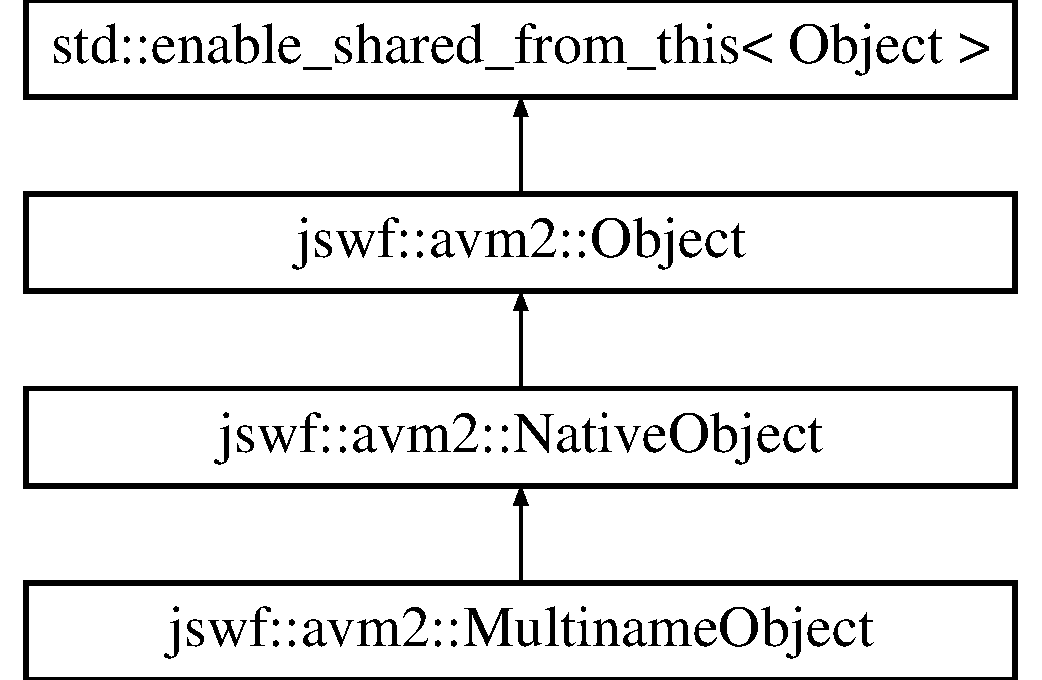
\includegraphics[height=4.000000cm]{classjswf_1_1avm2_1_1_multiname_object}
\end{center}
\end{figure}
\subsection*{Public Member Functions}
\begin{DoxyCompactItemize}
\item 
\hypertarget{classjswf_1_1avm2_1_1_multiname_object_adb163cbdc0e81445056fc4b311304e3e}{{\bfseries Multiname\+Object} (\hyperlink{classjswf_1_1avm2_1_1_v_m}{V\+M} $\ast$vm, const \hyperlink{structjswf_1_1avm2_1_1_multiname}{Multiname} \&value)}\label{classjswf_1_1avm2_1_1_multiname_object_adb163cbdc0e81445056fc4b311304e3e}

\item 
\hypertarget{classjswf_1_1avm2_1_1_multiname_object_ac1cd5835bb09899fca299c002505fcce}{\hyperlink{structjswf_1_1avm2_1_1_multiname}{Multiname} {\bfseries coerce\+\_\+multiname} () const }\label{classjswf_1_1avm2_1_1_multiname_object_ac1cd5835bb09899fca299c002505fcce}

\end{DoxyCompactItemize}
\subsection*{Public Attributes}
\begin{DoxyCompactItemize}
\item 
\hypertarget{classjswf_1_1avm2_1_1_multiname_object_a0e7a05691c60a91ab7024d184d53f6ff}{\hyperlink{structjswf_1_1avm2_1_1_multiname}{Multiname} {\bfseries value}}\label{classjswf_1_1avm2_1_1_multiname_object_a0e7a05691c60a91ab7024d184d53f6ff}

\end{DoxyCompactItemize}
\subsection*{Additional Inherited Members}


The documentation for this class was generated from the following files\+:\begin{DoxyCompactItemize}
\item 
jswf/avm2/Object.\+h\item 
jswf/avm2/Object.\+cpp\end{DoxyCompactItemize}

\hypertarget{structjswf_1_1avm2_1_1_namespace}{\section{jswf\+:\+:avm2\+:\+:Namespace Struct Reference}
\label{structjswf_1_1avm2_1_1_namespace}\index{jswf\+::avm2\+::\+Namespace@{jswf\+::avm2\+::\+Namespace}}
}
\subsection*{Public Member Functions}
\begin{DoxyCompactItemize}
\item 
\hypertarget{structjswf_1_1avm2_1_1_namespace_a1b472ce2b8702d0ddf267efe77be1287}{bool {\bfseries operator==} (const \hyperlink{structjswf_1_1avm2_1_1_namespace}{Namespace} \&rhs) const }\label{structjswf_1_1avm2_1_1_namespace_a1b472ce2b8702d0ddf267efe77be1287}

\item 
\hypertarget{structjswf_1_1avm2_1_1_namespace_aafb688482e05572d30aef1a32223db32}{bool {\bfseries operator!=} (const \hyperlink{structjswf_1_1avm2_1_1_namespace}{Namespace} \&rhs) const }\label{structjswf_1_1avm2_1_1_namespace_aafb688482e05572d30aef1a32223db32}

\end{DoxyCompactItemize}
\subsection*{Public Attributes}
\begin{DoxyCompactItemize}
\item 
\hypertarget{structjswf_1_1avm2_1_1_namespace_a77ed642d45f378cc58563c2975311c91}{Namespace\+Kind\+::\+Enum {\bfseries kind}}\label{structjswf_1_1avm2_1_1_namespace_a77ed642d45f378cc58563c2975311c91}

\item 
\hypertarget{structjswf_1_1avm2_1_1_namespace_ad9273b78cc67a2bbf514febb7c72691f}{\hyperlink{namespacejswf_a755127d61081aa8af105eb800aa2c1ec}{string} {\bfseries name}}\label{structjswf_1_1avm2_1_1_namespace_ad9273b78cc67a2bbf514febb7c72691f}

\end{DoxyCompactItemize}


The documentation for this struct was generated from the following file\+:\begin{DoxyCompactItemize}
\item 
jswf/avm2/Namespace.\+h\end{DoxyCompactItemize}

\hypertarget{structjswf_1_1avm2_1_1_namespace_kind}{\section{jswf\+:\+:avm2\+:\+:Namespace\+Kind Struct Reference}
\label{structjswf_1_1avm2_1_1_namespace_kind}\index{jswf\+::avm2\+::\+Namespace\+Kind@{jswf\+::avm2\+::\+Namespace\+Kind}}
}
\subsection*{Public Types}
\begin{DoxyCompactItemize}
\item 
\hypertarget{structjswf_1_1avm2_1_1_namespace_kind_a2a42f0e85fcb72dc05223c0720791aa8}{enum {\bfseries Enum} \+: u8\+\_\+t \{ \\*
{\bfseries Normal\+Namespace\+Kind} = 0x08, 
{\bfseries Package\+Namespace\+Kind} = 0x16, 
{\bfseries Package\+Internal\+Ns\+Kind} = 0x17, 
{\bfseries Protected\+Namespace\+Kind} = 0x18, 
\\*
{\bfseries Explicit\+Namespace\+Kind} = 0x19, 
{\bfseries Static\+Protected\+Ns\+Kind} = 0x1a, 
{\bfseries Private\+Namespace\+Kind} = 0x05
 \}}\label{structjswf_1_1avm2_1_1_namespace_kind_a2a42f0e85fcb72dc05223c0720791aa8}

\end{DoxyCompactItemize}


The documentation for this struct was generated from the following file\+:\begin{DoxyCompactItemize}
\item 
jswf/avm2/Namespace.\+h\end{DoxyCompactItemize}

\hypertarget{classjswf_1_1avm2_1_1_namespace_object}{\section{jswf\+:\+:avm2\+:\+:Namespace\+Object Class Reference}
\label{classjswf_1_1avm2_1_1_namespace_object}\index{jswf\+::avm2\+::\+Namespace\+Object@{jswf\+::avm2\+::\+Namespace\+Object}}
}
Inheritance diagram for jswf\+:\+:avm2\+:\+:Namespace\+Object\+:\begin{figure}[H]
\begin{center}
\leavevmode
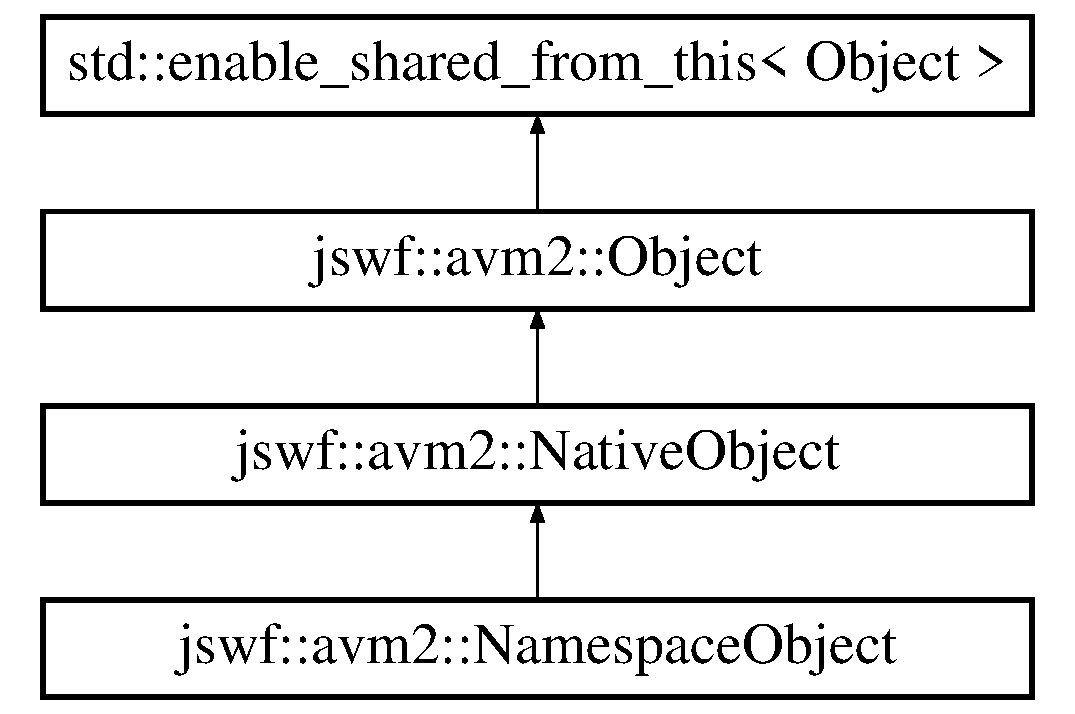
\includegraphics[height=4.000000cm]{classjswf_1_1avm2_1_1_namespace_object}
\end{center}
\end{figure}
\subsection*{Public Member Functions}
\begin{DoxyCompactItemize}
\item 
\hypertarget{classjswf_1_1avm2_1_1_namespace_object_a9b2ccd529b652b62df9b463780538072}{{\bfseries Namespace\+Object} (\hyperlink{classjswf_1_1avm2_1_1_v_m}{V\+M} $\ast$vm, const \hyperlink{structjswf_1_1avm2_1_1_namespace}{Namespace} \&value)}\label{classjswf_1_1avm2_1_1_namespace_object_a9b2ccd529b652b62df9b463780538072}

\item 
\hypertarget{classjswf_1_1avm2_1_1_namespace_object_a7e068d204be0abe49aac072622e2da20}{\hyperlink{structjswf_1_1avm2_1_1_namespace}{Namespace} {\bfseries coerce\+\_\+ns} () const }\label{classjswf_1_1avm2_1_1_namespace_object_a7e068d204be0abe49aac072622e2da20}

\end{DoxyCompactItemize}
\subsection*{Public Attributes}
\begin{DoxyCompactItemize}
\item 
\hypertarget{classjswf_1_1avm2_1_1_namespace_object_a3a71b9b39f57b88e0bd0f082a7936c66}{\hyperlink{structjswf_1_1avm2_1_1_namespace}{Namespace} {\bfseries value}}\label{classjswf_1_1avm2_1_1_namespace_object_a3a71b9b39f57b88e0bd0f082a7936c66}

\end{DoxyCompactItemize}
\subsection*{Additional Inherited Members}


The documentation for this class was generated from the following files\+:\begin{DoxyCompactItemize}
\item 
jswf/avm2/Object.\+h\item 
jswf/avm2/Object.\+cpp\end{DoxyCompactItemize}

\hypertarget{structjswf_1_1avm2_1_1_namespace_set}{\section{jswf\+:\+:avm2\+:\+:Namespace\+Set Struct Reference}
\label{structjswf_1_1avm2_1_1_namespace_set}\index{jswf\+::avm2\+::\+Namespace\+Set@{jswf\+::avm2\+::\+Namespace\+Set}}
}
\subsection*{Public Member Functions}
\begin{DoxyCompactItemize}
\item 
\hypertarget{structjswf_1_1avm2_1_1_namespace_set_a3701a3ce565076949258e7e3fb29c994}{bool {\bfseries operator==} (const \hyperlink{structjswf_1_1avm2_1_1_namespace_set}{Namespace\+Set} \&rhs) const }\label{structjswf_1_1avm2_1_1_namespace_set_a3701a3ce565076949258e7e3fb29c994}

\item 
\hypertarget{structjswf_1_1avm2_1_1_namespace_set_af889b4a06bb318fe7c77db5cfb35a2d8}{bool {\bfseries operator!=} (const \hyperlink{structjswf_1_1avm2_1_1_namespace_set}{Namespace\+Set} \&rhs) const }\label{structjswf_1_1avm2_1_1_namespace_set_af889b4a06bb318fe7c77db5cfb35a2d8}

\end{DoxyCompactItemize}
\subsection*{Public Attributes}
\begin{DoxyCompactItemize}
\item 
\hypertarget{structjswf_1_1avm2_1_1_namespace_set_a16072c17ace3c487a85b47494c3050dc}{std\+::vector$<$ Namespace\+Ptr $>$ {\bfseries namespaces}}\label{structjswf_1_1avm2_1_1_namespace_set_a16072c17ace3c487a85b47494c3050dc}

\end{DoxyCompactItemize}


The documentation for this struct was generated from the following file\+:\begin{DoxyCompactItemize}
\item 
jswf/avm2/Namespace.\+h\end{DoxyCompactItemize}

\hypertarget{classjswf_1_1avm2_1_1_native_object}{\section{jswf\+:\+:avm2\+:\+:Native\+Object Class Reference}
\label{classjswf_1_1avm2_1_1_native_object}\index{jswf\+::avm2\+::\+Native\+Object@{jswf\+::avm2\+::\+Native\+Object}}
}
Inheritance diagram for jswf\+:\+:avm2\+:\+:Native\+Object\+:\begin{figure}[H]
\begin{center}
\leavevmode
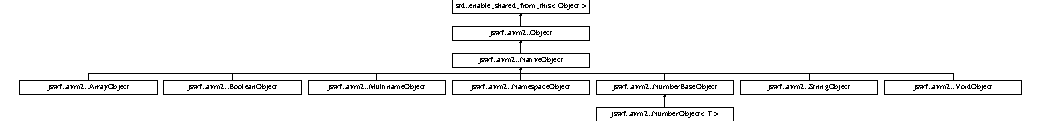
\includegraphics[height=1.632653cm]{classjswf_1_1avm2_1_1_native_object}
\end{center}
\end{figure}
\subsection*{Public Member Functions}
\begin{DoxyCompactItemize}
\item 
\hypertarget{classjswf_1_1avm2_1_1_native_object_a0bd86d5ad15cc3b4ffcc88ece5024f04}{{\bfseries Native\+Object} (\hyperlink{classjswf_1_1avm2_1_1_v_m}{V\+M} $\ast$vm, \hyperlink{classjswf_1_1avm2_1_1_class}{Class} $\ast$klass)}\label{classjswf_1_1avm2_1_1_native_object_a0bd86d5ad15cc3b4ffcc88ece5024f04}

\item 
\hypertarget{classjswf_1_1avm2_1_1_native_object_a275a3cd12c6c195d51731deace28fcad}{virtual std\+::shared\+\_\+ptr$<$ const \\*
\hyperlink{classjswf_1_1avm2_1_1_object}{Object} $>$ {\bfseries ecma\+To\+Primitive} (E\+C\+M\+A\+Hint\+::\+Enum hint=E\+C\+M\+A\+Hint\+::\+No\+Hint) const }\label{classjswf_1_1avm2_1_1_native_object_a275a3cd12c6c195d51731deace28fcad}

\end{DoxyCompactItemize}
\subsection*{Additional Inherited Members}


The documentation for this class was generated from the following file\+:\begin{DoxyCompactItemize}
\item 
jswf/avm2/Object.\+h\end{DoxyCompactItemize}

\hypertarget{classjswf_1_1avm2_1_1ast_1_1_node}{\section{jswf\+:\+:avm2\+:\+:ast\+:\+:Node Class Reference}
\label{classjswf_1_1avm2_1_1ast_1_1_node}\index{jswf\+::avm2\+::ast\+::\+Node@{jswf\+::avm2\+::ast\+::\+Node}}
}


Serves as super-\/class for all nodes.  




{\ttfamily \#include $<$Node.\+h$>$}

Inheritance diagram for jswf\+:\+:avm2\+:\+:ast\+:\+:Node\+:\begin{figure}[H]
\begin{center}
\leavevmode
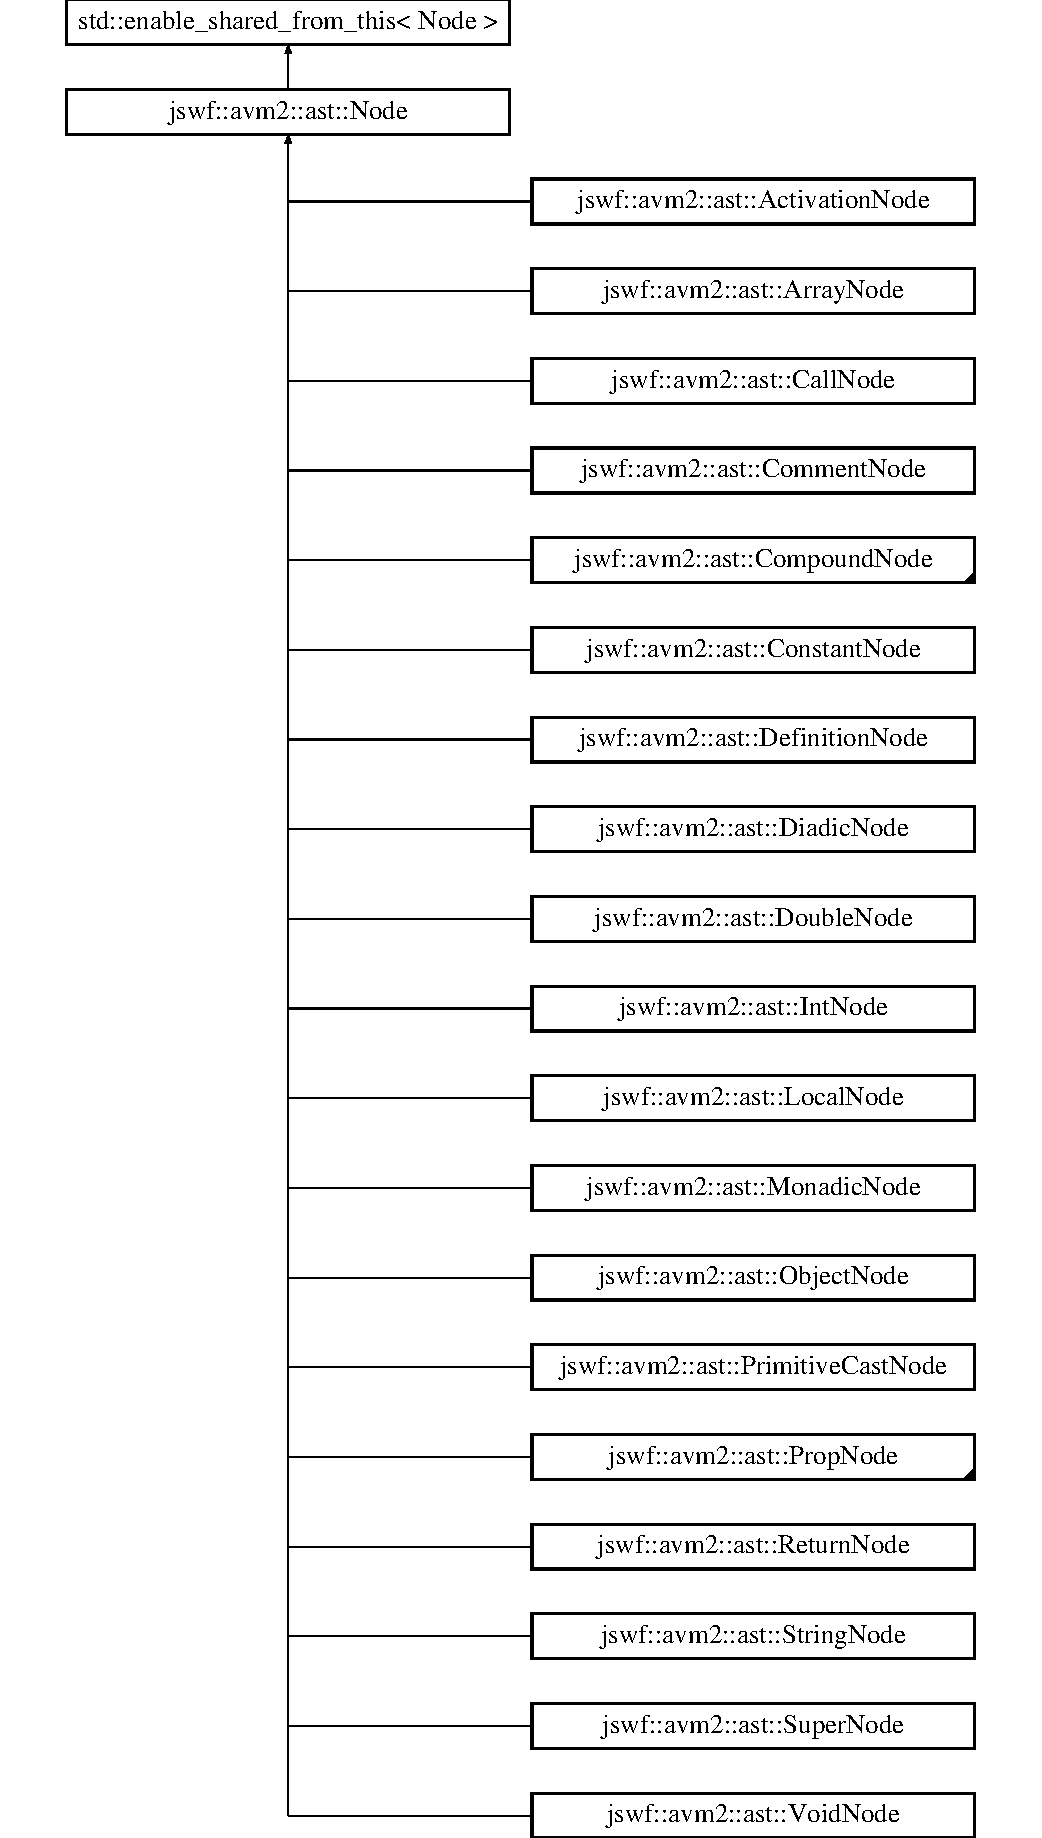
\includegraphics[height=12.000000cm]{classjswf_1_1avm2_1_1ast_1_1_node}
\end{center}
\end{figure}
\subsection*{Public Member Functions}
\begin{DoxyCompactItemize}
\item 
\hypertarget{classjswf_1_1avm2_1_1ast_1_1_node_a46fe59a6cc17db632f9ba30822fb3aa8}{{\bfseries Node} (int precedence)}\label{classjswf_1_1avm2_1_1ast_1_1_node_a46fe59a6cc17db632f9ba30822fb3aa8}

\item 
\hypertarget{classjswf_1_1avm2_1_1ast_1_1_node_a51999c6e386f245932a10c1113bcc1da}{virtual std\+::string {\bfseries to\+String} ()=0}\label{classjswf_1_1avm2_1_1ast_1_1_node_a51999c6e386f245932a10c1113bcc1da}

\item 
\hypertarget{classjswf_1_1avm2_1_1ast_1_1_node_accc224a86b8763b8118eada587a8d3f0}{std\+::string {\bfseries coerce\+\_\+s} ()}\label{classjswf_1_1avm2_1_1ast_1_1_node_accc224a86b8763b8118eada587a8d3f0}

\item 
\hypertarget{classjswf_1_1avm2_1_1ast_1_1_node_ab9b58f5ac7724aea72c7cfe915e26160}{\hyperlink{structjswf_1_1avm2_1_1_namespace}{Namespace} {\bfseries coerce\+\_\+ns} ()}\label{classjswf_1_1avm2_1_1ast_1_1_node_ab9b58f5ac7724aea72c7cfe915e26160}

\item 
\hypertarget{classjswf_1_1avm2_1_1ast_1_1_node_a7b5a29af1daaa743edb692f2cc1c5406}{virtual std\+::string {\bfseries to\+Intended\+String} (int intend)}\label{classjswf_1_1avm2_1_1ast_1_1_node_a7b5a29af1daaa743edb692f2cc1c5406}

\item 
\hypertarget{classjswf_1_1avm2_1_1ast_1_1_node_a448c422f0c108a0b2a76b03b991421e9}{std\+::shared\+\_\+ptr$<$ \hyperlink{classjswf_1_1avm2_1_1ast_1_1_node}{Node} $>$ {\bfseries get\+Property} (\hyperlink{structjswf_1_1avm2_1_1_multiname}{Multiname} \&mn)}\label{classjswf_1_1avm2_1_1ast_1_1_node_a448c422f0c108a0b2a76b03b991421e9}

\item 
\hypertarget{classjswf_1_1avm2_1_1ast_1_1_node_a5df00f84b7f6416cbe892c3fd4144c5d}{std\+::shared\+\_\+ptr$<$ \hyperlink{classjswf_1_1avm2_1_1ast_1_1_node}{Node} $>$ {\bfseries set\+Property} (\hyperlink{structjswf_1_1avm2_1_1_multiname}{Multiname} \&mn, std\+::shared\+\_\+ptr$<$ \hyperlink{classjswf_1_1avm2_1_1ast_1_1_node}{Node} $>$ \&value)}\label{classjswf_1_1avm2_1_1ast_1_1_node_a5df00f84b7f6416cbe892c3fd4144c5d}

\end{DoxyCompactItemize}
\subsection*{Public Attributes}
\begin{DoxyCompactItemize}
\item 
\hypertarget{classjswf_1_1avm2_1_1ast_1_1_node_a2c3c6d68bbd9448af7aeb068c51a3309}{int {\bfseries precedence}}\label{classjswf_1_1avm2_1_1ast_1_1_node_a2c3c6d68bbd9448af7aeb068c51a3309}

\end{DoxyCompactItemize}


\subsection{Detailed Description}
Serves as super-\/class for all nodes. 

The documentation for this class was generated from the following files\+:\begin{DoxyCompactItemize}
\item 
jswf/avm2/ast/Node.\+h\item 
jswf/avm2/ast/Node.\+cpp\end{DoxyCompactItemize}

\hypertarget{classjswf_1_1avm2_1_1_number_base_object}{\section{jswf\+:\+:avm2\+:\+:Number\+Base\+Object Class Reference}
\label{classjswf_1_1avm2_1_1_number_base_object}\index{jswf\+::avm2\+::\+Number\+Base\+Object@{jswf\+::avm2\+::\+Number\+Base\+Object}}
}
Inheritance diagram for jswf\+:\+:avm2\+:\+:Number\+Base\+Object\+:\begin{figure}[H]
\begin{center}
\leavevmode
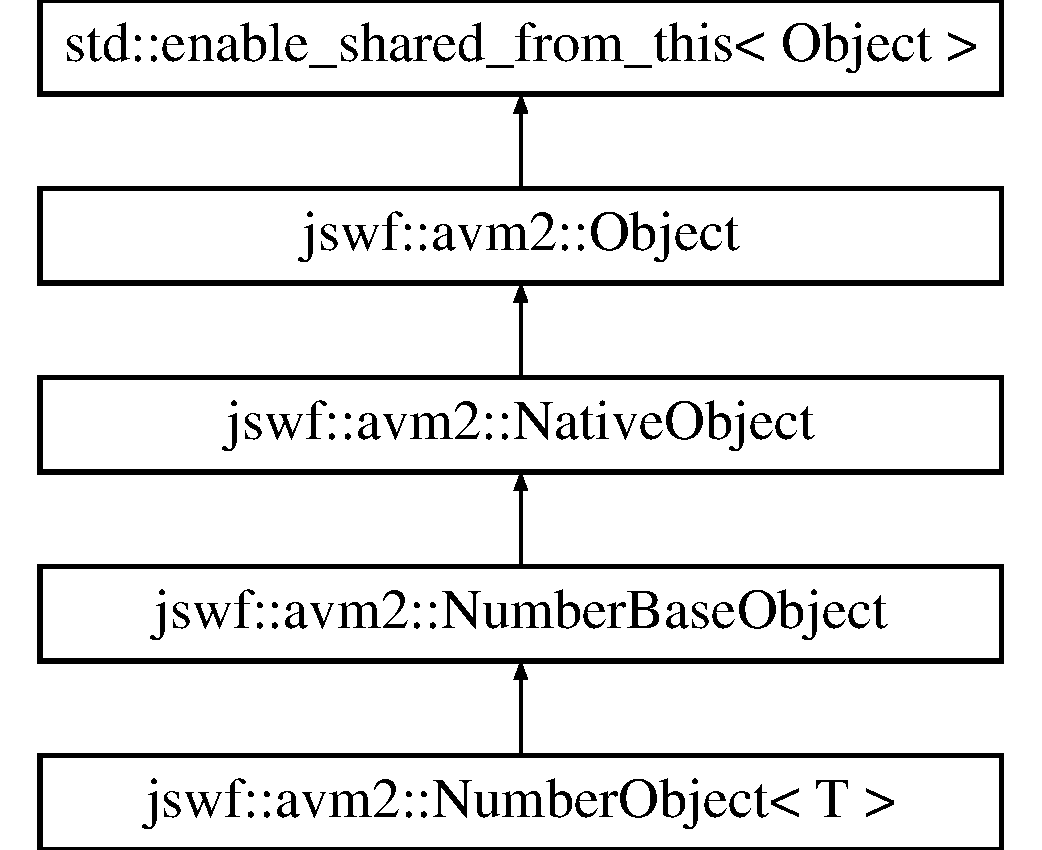
\includegraphics[height=5.000000cm]{classjswf_1_1avm2_1_1_number_base_object}
\end{center}
\end{figure}
\subsection*{Public Member Functions}
\begin{DoxyCompactItemize}
\item 
\hypertarget{classjswf_1_1avm2_1_1_number_base_object_a092789e5e3e6662ea076b3209d4cad7b}{{\bfseries Number\+Base\+Object} (\hyperlink{classjswf_1_1avm2_1_1_v_m}{V\+M} $\ast$vm, \hyperlink{classjswf_1_1avm2_1_1_class}{Class} $\ast$klass)}\label{classjswf_1_1avm2_1_1_number_base_object_a092789e5e3e6662ea076b3209d4cad7b}

\end{DoxyCompactItemize}
\subsection*{Additional Inherited Members}


The documentation for this class was generated from the following file\+:\begin{DoxyCompactItemize}
\item 
jswf/avm2/Object.\+h\end{DoxyCompactItemize}

\hypertarget{classjswf_1_1avm2_1_1_number_object}{\section{jswf\+:\+:avm2\+:\+:Number\+Object$<$ T $>$ Class Template Reference}
\label{classjswf_1_1avm2_1_1_number_object}\index{jswf\+::avm2\+::\+Number\+Object$<$ T $>$@{jswf\+::avm2\+::\+Number\+Object$<$ T $>$}}
}


Represents a number (E\+C\+M\+A-\/262, section 8.\+5 {\itshape The Number Type}), backed using type {\ttfamily T}.  




{\ttfamily \#include $<$Object.\+h$>$}

Inheritance diagram for jswf\+:\+:avm2\+:\+:Number\+Object$<$ T $>$\+:\begin{figure}[H]
\begin{center}
\leavevmode
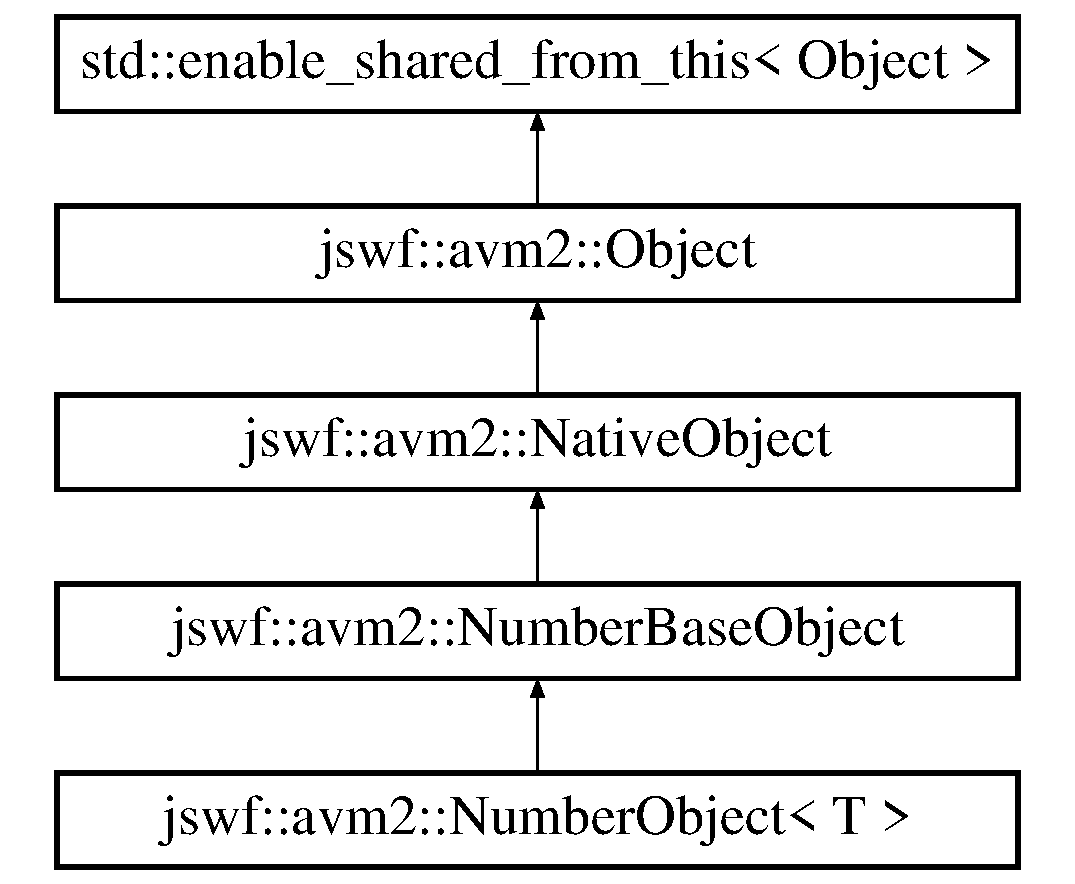
\includegraphics[height=5.000000cm]{classjswf_1_1avm2_1_1_number_object}
\end{center}
\end{figure}
\subsection*{Public Member Functions}
\begin{DoxyCompactItemize}
\item 
\hypertarget{classjswf_1_1avm2_1_1_number_object_afd6f25846d1060b5cc179048e0c94b33}{{\bfseries Number\+Object} (\hyperlink{classjswf_1_1avm2_1_1_v_m}{V\+M} $\ast$vm, const T \&value)}\label{classjswf_1_1avm2_1_1_number_object_afd6f25846d1060b5cc179048e0c94b33}

\item 
\hypertarget{classjswf_1_1avm2_1_1_number_object_a2514993b781c018e62cb53dba51378ad}{bool \hyperlink{classjswf_1_1avm2_1_1_number_object_a2514993b781c018e62cb53dba51378ad}{coerce\+\_\+b} () const }\label{classjswf_1_1avm2_1_1_number_object_a2514993b781c018e62cb53dba51378ad}

\begin{DoxyCompactList}\small\item\em Converts to {\ttfamily bool} (E\+C\+M\+A-\/262, section 9.\+2 {\itshape To\+Boolean}) \end{DoxyCompactList}\item 
std\+::string \hyperlink{classjswf_1_1avm2_1_1_number_object_ae739a9db414d4c5924faaa549384a24c}{coerce\+\_\+s} () const 
\begin{DoxyCompactList}\small\item\em Converts to {\ttfamily std\+::string} (E\+C\+M\+A-\/262, section 9.\+8 {\itshape To\+String}) \end{DoxyCompactList}\item 
\hypertarget{classjswf_1_1avm2_1_1_number_object_a46b26e8ee57e4140d830196b50ea5714}{double \hyperlink{classjswf_1_1avm2_1_1_number_object_a46b26e8ee57e4140d830196b50ea5714}{coerce\+\_\+d} () const }\label{classjswf_1_1avm2_1_1_number_object_a46b26e8ee57e4140d830196b50ea5714}

\begin{DoxyCompactList}\small\item\em Converts to {\ttfamily double} (E\+C\+M\+A-\/262, section 9.\+3 {\itshape To\+Number}) \end{DoxyCompactList}\item 
\hypertarget{classjswf_1_1avm2_1_1_number_object_a227caf4e09dbbb48af123db295455a95}{bool {\bfseries same\+Type\+Equals} (const \hyperlink{classjswf_1_1avm2_1_1_object}{Object} \&rhs) const }\label{classjswf_1_1avm2_1_1_number_object_a227caf4e09dbbb48af123db295455a95}

\item 
\hypertarget{classjswf_1_1avm2_1_1_number_object_a9831edc4607ba7ff6773911b48ca7eec}{bool {\bfseries same\+Type\+Strict\+Equals} (const \hyperlink{classjswf_1_1avm2_1_1_object}{Object} \&rhs) const }\label{classjswf_1_1avm2_1_1_number_object_a9831edc4607ba7ff6773911b48ca7eec}

\end{DoxyCompactItemize}
\subsection*{Public Attributes}
\begin{DoxyCompactItemize}
\item 
\hypertarget{classjswf_1_1avm2_1_1_number_object_a21662f9bfc7c8f6f927c1e9008e177a0}{T {\bfseries value}}\label{classjswf_1_1avm2_1_1_number_object_a21662f9bfc7c8f6f927c1e9008e177a0}

\end{DoxyCompactItemize}
\subsection*{Additional Inherited Members}


\subsection{Detailed Description}
\subsubsection*{template$<$typename T$>$class jswf\+::avm2\+::\+Number\+Object$<$ T $>$}

Represents a number (E\+C\+M\+A-\/262, section 8.\+5 {\itshape The Number Type}), backed using type {\ttfamily T}. 

\subsection{Member Function Documentation}
\hypertarget{classjswf_1_1avm2_1_1_number_object_ae739a9db414d4c5924faaa549384a24c}{\index{jswf\+::avm2\+::\+Number\+Object@{jswf\+::avm2\+::\+Number\+Object}!coerce\+\_\+s@{coerce\+\_\+s}}
\index{coerce\+\_\+s@{coerce\+\_\+s}!jswf\+::avm2\+::\+Number\+Object@{jswf\+::avm2\+::\+Number\+Object}}
\subsubsection[{coerce\+\_\+s}]{\setlength{\rightskip}{0pt plus 5cm}template$<$typename T $>$ std\+::string {\bf jswf\+::avm2\+::\+Number\+Object}$<$ T $>$\+::coerce\+\_\+s (
\begin{DoxyParamCaption}
{}
\end{DoxyParamCaption}
) const\hspace{0.3cm}{\ttfamily [inline]}, {\ttfamily [virtual]}}}\label{classjswf_1_1avm2_1_1_number_object_ae739a9db414d4c5924faaa549384a24c}


Converts to {\ttfamily std\+::string} (E\+C\+M\+A-\/262, section 9.\+8 {\itshape To\+String}) 

\begin{DoxyRefDesc}{Todo}
\item[\hyperlink{todo__todo000007}{Todo}]Implement 9.\+8.\+1 \end{DoxyRefDesc}


Reimplemented from \hyperlink{classjswf_1_1avm2_1_1_object_a69b39776062acaccd2cd2b5a1f937c9d}{jswf\+::avm2\+::\+Object}.



The documentation for this class was generated from the following files\+:\begin{DoxyCompactItemize}
\item 
jswf/avm2/Object.\+h\item 
jswf/avm2/Object.\+cpp\end{DoxyCompactItemize}

\hypertarget{classjswf_1_1avm2_1_1_object}{\section{jswf\+:\+:avm2\+:\+:Object Class Reference}
\label{classjswf_1_1avm2_1_1_object}\index{jswf\+::avm2\+::\+Object@{jswf\+::avm2\+::\+Object}}
}
Inheritance diagram for jswf\+:\+:avm2\+:\+:Object\+:\begin{figure}[H]
\begin{center}
\leavevmode
\includegraphics[height=1.269841cm]{classjswf_1_1avm2_1_1_object}
\end{center}
\end{figure}
\subsection*{Public Types}
\begin{DoxyCompactItemize}
\item 
\hypertarget{classjswf_1_1avm2_1_1_object_a5a091b9c7f6a6618eafca72f20687c77}{enum {\bfseries Ac\+Result} \{ {\bfseries Ac\+Undefined\+Result} = 0, 
{\bfseries Ac\+False\+Result} = 1, 
{\bfseries Ac\+True\+Result} = 2
 \}}\label{classjswf_1_1avm2_1_1_object_a5a091b9c7f6a6618eafca72f20687c77}

\end{DoxyCompactItemize}
\subsection*{Public Member Functions}
\begin{DoxyCompactItemize}
\item 
\hypertarget{classjswf_1_1avm2_1_1_object_abb25a126cb469bfd01fbbf193175f365}{{\bfseries Object} (\hyperlink{classjswf_1_1avm2_1_1_v_m}{V\+M} $\ast$vm, \hyperlink{classjswf_1_1avm2_1_1_class}{Class} $\ast$klass)}\label{classjswf_1_1avm2_1_1_object_abb25a126cb469bfd01fbbf193175f365}

\item 
\hypertarget{classjswf_1_1avm2_1_1_object_a0bcf1f52a7f769165afa385bbe4af929}{uint16\+\_\+t \hyperlink{classjswf_1_1avm2_1_1_object_a0bcf1f52a7f769165afa385bbe4af929}{coerce\+\_\+u16} () const }\label{classjswf_1_1avm2_1_1_object_a0bcf1f52a7f769165afa385bbe4af929}

\begin{DoxyCompactList}\small\item\em Converts to {\ttfamily uint16\+\_\+t} (E\+C\+M\+A-\/262, section 9.\+7 {\itshape To\+Uint16}) \end{DoxyCompactList}\item 
\hypertarget{classjswf_1_1avm2_1_1_object_ad43d5df01cf90a380407c4b2e7e55347}{uint32\+\_\+t \hyperlink{classjswf_1_1avm2_1_1_object_ad43d5df01cf90a380407c4b2e7e55347}{coerce\+\_\+u32} () const }\label{classjswf_1_1avm2_1_1_object_ad43d5df01cf90a380407c4b2e7e55347}

\begin{DoxyCompactList}\small\item\em Converts to {\ttfamily uint32\+\_\+t} (E\+C\+M\+A-\/262, section 9.\+6 {\itshape To\+Uint32}) \end{DoxyCompactList}\item 
\hypertarget{classjswf_1_1avm2_1_1_object_a8964127c38a8062255a9c011fde3d00b}{int32\+\_\+t \hyperlink{classjswf_1_1avm2_1_1_object_a8964127c38a8062255a9c011fde3d00b}{coerce\+\_\+s32} () const }\label{classjswf_1_1avm2_1_1_object_a8964127c38a8062255a9c011fde3d00b}

\begin{DoxyCompactList}\small\item\em Converts to {\ttfamily int32\+\_\+t} (E\+C\+M\+A-\/262, section 9.\+5 {\itshape To\+Int32}) \end{DoxyCompactList}\item 
\hypertarget{classjswf_1_1avm2_1_1_object_a90d8bccb705b510a015a7a3976aedd71}{\hyperlink{structjswf_1_1avm2_1_1_trait_match}{Trait\+Match} {\bfseries get\+Trait\+By\+Name} (const \hyperlink{structjswf_1_1avm2_1_1_multiname}{Multiname} \&name)}\label{classjswf_1_1avm2_1_1_object_a90d8bccb705b510a015a7a3976aedd71}

\item 
\hypertarget{classjswf_1_1avm2_1_1_object_a131cc416f028567451a06dee37966b72}{\hyperlink{structjswf_1_1avm2_1_1_trait_match}{Trait\+Match} {\bfseries get\+Trait\+By\+Slot\+Id} (\hyperlink{namespacejswf_aa10d9ddca2a6a5debdc261dfae3d1117}{u30\+\_\+t} slot\+Id)}\label{classjswf_1_1avm2_1_1_object_a131cc416f028567451a06dee37966b72}

\item 
\hypertarget{classjswf_1_1avm2_1_1_object_afda0bad45f86f4d69c2466c863528160}{virtual Object\+Ptr {\bfseries get\+Property} (const \hyperlink{structjswf_1_1avm2_1_1_multiname}{Multiname} \&property)}\label{classjswf_1_1avm2_1_1_object_afda0bad45f86f4d69c2466c863528160}

\item 
\hypertarget{classjswf_1_1avm2_1_1_object_a1dec9b414e64bd9635a86d5f47379f2f}{virtual void {\bfseries set\+Property} (const \hyperlink{structjswf_1_1avm2_1_1_multiname}{Multiname} \&property, const Object\+Ptr \&value)}\label{classjswf_1_1avm2_1_1_object_a1dec9b414e64bd9635a86d5f47379f2f}

\item 
\hypertarget{classjswf_1_1avm2_1_1_object_af7ce6421f0fb63694d83993d8a1e0b77}{void {\bfseries set\+Slot} (\hyperlink{namespacejswf_aa10d9ddca2a6a5debdc261dfae3d1117}{u30\+\_\+t} slot\+Index, const Object\+Ptr \&value)}\label{classjswf_1_1avm2_1_1_object_af7ce6421f0fb63694d83993d8a1e0b77}

\item 
\hypertarget{classjswf_1_1avm2_1_1_object_ad5d5b6a0f60b7a0ae41304753c8c6fdc}{Object\+Ptr {\bfseries get\+Slot} (\hyperlink{namespacejswf_aa10d9ddca2a6a5debdc261dfae3d1117}{u30\+\_\+t} slot\+Index) const }\label{classjswf_1_1avm2_1_1_object_ad5d5b6a0f60b7a0ae41304753c8c6fdc}

\item 
\hypertarget{classjswf_1_1avm2_1_1_object_a3d2b390062f97d6f563eabdc59dff3e9}{virtual Object\+Ptr {\bfseries ecma\+Call} (\hyperlink{classjswf_1_1avm2_1_1_v_m}{V\+M} \&vm, std\+::vector$<$ Object\+Ptr $>$ \&args) const }\label{classjswf_1_1avm2_1_1_object_a3d2b390062f97d6f563eabdc59dff3e9}

\item 
\hypertarget{classjswf_1_1avm2_1_1_object_a68d84b207f96c834586769298b4037e9}{bool {\bfseries has\+Declared\+Property} (const \hyperlink{structjswf_1_1avm2_1_1_multiname}{Multiname} \&property)}\label{classjswf_1_1avm2_1_1_object_a68d84b207f96c834586769298b4037e9}

\item 
\hypertarget{classjswf_1_1avm2_1_1_object_a895e66d35dae4e698abd24d444f82e75}{bool {\bfseries has\+Dynamic\+Property} (const \hyperlink{structjswf_1_1avm2_1_1_multiname}{Multiname} \&property)}\label{classjswf_1_1avm2_1_1_object_a895e66d35dae4e698abd24d444f82e75}

\item 
\hypertarget{classjswf_1_1avm2_1_1_object_a821095f562e988e8e571e3760cdb9c62}{bool {\bfseries has\+Property} (const \hyperlink{structjswf_1_1avm2_1_1_multiname}{Multiname} \&property)}\label{classjswf_1_1avm2_1_1_object_a821095f562e988e8e571e3760cdb9c62}

\item 
\hypertarget{classjswf_1_1avm2_1_1_object_a02abb4413a3109b38cf9b7b65409e37f}{virtual std\+::string {\bfseries to\+String} () const }\label{classjswf_1_1avm2_1_1_object_a02abb4413a3109b38cf9b7b65409e37f}

\item 
\hypertarget{classjswf_1_1avm2_1_1_object_a62a6bcbb6a7efde92e8999095ed382c3}{virtual bool {\bfseries same\+Type\+Equals} (const \hyperlink{classjswf_1_1avm2_1_1_object}{Object} \&rhs) const }\label{classjswf_1_1avm2_1_1_object_a62a6bcbb6a7efde92e8999095ed382c3}

\item 
\hypertarget{classjswf_1_1avm2_1_1_object_a8120f3a2e595bede5b19bba58324e3ab}{virtual bool {\bfseries operator==} (const \hyperlink{classjswf_1_1avm2_1_1_object}{Object} \&rhs) const }\label{classjswf_1_1avm2_1_1_object_a8120f3a2e595bede5b19bba58324e3ab}

\item 
\hypertarget{classjswf_1_1avm2_1_1_object_aba9196c91303634b0c10f2646ec92531}{virtual bool {\bfseries operator!=} (const \hyperlink{classjswf_1_1avm2_1_1_object}{Object} \&rhs) const }\label{classjswf_1_1avm2_1_1_object_aba9196c91303634b0c10f2646ec92531}

\item 
\hypertarget{classjswf_1_1avm2_1_1_object_a9c551db7f14dd6d62f2264b48fec42a0}{virtual bool {\bfseries operator$<$} (const \hyperlink{classjswf_1_1avm2_1_1_object}{Object} \&rhs) const }\label{classjswf_1_1avm2_1_1_object_a9c551db7f14dd6d62f2264b48fec42a0}

\item 
\hypertarget{classjswf_1_1avm2_1_1_object_aa400d6c688e61271c7393a4e99ee3852}{virtual bool {\bfseries operator$>$} (const \hyperlink{classjswf_1_1avm2_1_1_object}{Object} \&rhs) const }\label{classjswf_1_1avm2_1_1_object_aa400d6c688e61271c7393a4e99ee3852}

\item 
\hypertarget{classjswf_1_1avm2_1_1_object_a16a905fd555a59ce1d29e76746e940b4}{virtual bool {\bfseries operator$<$=} (const \hyperlink{classjswf_1_1avm2_1_1_object}{Object} \&rhs) const }\label{classjswf_1_1avm2_1_1_object_a16a905fd555a59ce1d29e76746e940b4}

\item 
\hypertarget{classjswf_1_1avm2_1_1_object_a845c7fd546cfa0129338639a228be363}{virtual bool {\bfseries operator$>$=} (const \hyperlink{classjswf_1_1avm2_1_1_object}{Object} \&rhs) const }\label{classjswf_1_1avm2_1_1_object_a845c7fd546cfa0129338639a228be363}

\item 
\hypertarget{classjswf_1_1avm2_1_1_object_a85dfccddcf99772ffe3fa160c8cff935}{virtual bool {\bfseries same\+Type\+Strict\+Equals} (const \hyperlink{classjswf_1_1avm2_1_1_object}{Object} \&rhs) const }\label{classjswf_1_1avm2_1_1_object_a85dfccddcf99772ffe3fa160c8cff935}

\item 
\hypertarget{classjswf_1_1avm2_1_1_object_ae88ca0d26efbb597791a8e72dbf7b267}{virtual bool {\bfseries strict\+Equals} (const \hyperlink{classjswf_1_1avm2_1_1_object}{Object} \&rhs) const }\label{classjswf_1_1avm2_1_1_object_ae88ca0d26efbb597791a8e72dbf7b267}

\item 
\hypertarget{classjswf_1_1avm2_1_1_object_a98bb4755912f958f91f18b19c889aa49}{virtual std\+::shared\+\_\+ptr$<$ const \\*
\hyperlink{classjswf_1_1avm2_1_1_object}{Object} $>$ {\bfseries ecma\+To\+Primitive} (E\+C\+M\+A\+Hint\+::\+Enum hint=E\+C\+M\+A\+Hint\+::\+No\+Hint) const }\label{classjswf_1_1avm2_1_1_object_a98bb4755912f958f91f18b19c889aa49}

\item 
\hypertarget{classjswf_1_1avm2_1_1_object_ad4f91847c647ebda6984d93add7e3e2d}{virtual Object\+Ptr \hyperlink{classjswf_1_1avm2_1_1_object_ad4f91847c647ebda6984d93add7e3e2d}{ecma\+To\+Primitive} (E\+C\+M\+A\+Hint\+::\+Enum hint=E\+C\+M\+A\+Hint\+::\+No\+Hint)}\label{classjswf_1_1avm2_1_1_object_ad4f91847c647ebda6984d93add7e3e2d}

\begin{DoxyCompactList}\small\item\em Converts to a primitive object (subclass of \hyperlink{classjswf_1_1avm2_1_1_native_object}{Native\+Object}) (E\+C\+M\+A-\/262, section 9.\+1 {\itshape To\+Primitive}) \end{DoxyCompactList}\item 
\hypertarget{classjswf_1_1avm2_1_1_object_aca334088631f4dc1c49df9d93a806829}{virtual bool \hyperlink{classjswf_1_1avm2_1_1_object_aca334088631f4dc1c49df9d93a806829}{coerce\+\_\+b} () const }\label{classjswf_1_1avm2_1_1_object_aca334088631f4dc1c49df9d93a806829}

\begin{DoxyCompactList}\small\item\em Converts to {\ttfamily bool} (E\+C\+M\+A-\/262, section 9.\+2 {\itshape To\+Boolean}) \end{DoxyCompactList}\item 
virtual std\+::string \hyperlink{classjswf_1_1avm2_1_1_object_a69b39776062acaccd2cd2b5a1f937c9d}{coerce\+\_\+s} () const 
\begin{DoxyCompactList}\small\item\em Converts to {\ttfamily std\+::string} (E\+C\+M\+A-\/262, section 9.\+8 {\itshape To\+String}) \end{DoxyCompactList}\item 
\hypertarget{classjswf_1_1avm2_1_1_object_ae70efbb4c5dc0506dd0f25aa2edc7033}{virtual \hyperlink{structjswf_1_1avm2_1_1_namespace}{Namespace} {\bfseries coerce\+\_\+ns} () const }\label{classjswf_1_1avm2_1_1_object_ae70efbb4c5dc0506dd0f25aa2edc7033}

\item 
\hypertarget{classjswf_1_1avm2_1_1_object_ad060c6ca029ad1158173bd2f20a6bd07}{virtual \hyperlink{structjswf_1_1avm2_1_1_multiname}{Multiname} {\bfseries coerce\+\_\+multiname} () const }\label{classjswf_1_1avm2_1_1_object_ad060c6ca029ad1158173bd2f20a6bd07}

\item 
\hypertarget{classjswf_1_1avm2_1_1_object_ac2804e1879e170ae43cea1f17efbb7e8}{virtual double \hyperlink{classjswf_1_1avm2_1_1_object_ac2804e1879e170ae43cea1f17efbb7e8}{coerce\+\_\+d} () const }\label{classjswf_1_1avm2_1_1_object_ac2804e1879e170ae43cea1f17efbb7e8}

\begin{DoxyCompactList}\small\item\em Converts to {\ttfamily double} (E\+C\+M\+A-\/262, section 9.\+3 {\itshape To\+Number}) \end{DoxyCompactList}\item 
\hypertarget{classjswf_1_1avm2_1_1_object_afedcb68d25763184499b1c7c0ea99c7d}{virtual Object\+Ptr {\bfseries coerce} (\hyperlink{classjswf_1_1avm2_1_1_class}{Class} $\ast$new\+Klass)}\label{classjswf_1_1avm2_1_1_object_afedcb68d25763184499b1c7c0ea99c7d}

\item 
\hypertarget{classjswf_1_1avm2_1_1_object_a2eaa32c64fedbb664b5531a2c7e7dbb5}{std\+::string {\bfseries get\+Property\+Name} (int index) const }\label{classjswf_1_1avm2_1_1_object_a2eaa32c64fedbb664b5531a2c7e7dbb5}

\item 
\hypertarget{classjswf_1_1avm2_1_1_object_acb1bda095198b9996549b227428403c0}{bool {\bfseries has\+Next\+Property} (int index) const }\label{classjswf_1_1avm2_1_1_object_acb1bda095198b9996549b227428403c0}

\end{DoxyCompactItemize}
\subsection*{Static Public Member Functions}
\begin{DoxyCompactItemize}
\item 
\hypertarget{classjswf_1_1avm2_1_1_object_acbeac16ed3dcedf342afe5ec12d928c9}{static Ac\+Result {\bfseries ecma\+Abstract\+Compare} (const \hyperlink{classjswf_1_1avm2_1_1_object}{Object} \&lhs, const \hyperlink{classjswf_1_1avm2_1_1_object}{Object} \&rhs, bool left\+First=true)}\label{classjswf_1_1avm2_1_1_object_acbeac16ed3dcedf342afe5ec12d928c9}

\end{DoxyCompactItemize}
\subsection*{Public Attributes}
\begin{DoxyCompactItemize}
\item 
\hypertarget{classjswf_1_1avm2_1_1_object_adf9ff969fcf2e2ab376b1728ceeee19a}{\hyperlink{classjswf_1_1avm2_1_1_v_m}{V\+M} $\ast$ {\bfseries vm}}\label{classjswf_1_1avm2_1_1_object_adf9ff969fcf2e2ab376b1728ceeee19a}

\item 
\hypertarget{classjswf_1_1avm2_1_1_object_a1ac6b806f384717a84531e7324f56759}{\hyperlink{classjswf_1_1avm2_1_1_class}{Class} $\ast$ {\bfseries klass}}\label{classjswf_1_1avm2_1_1_object_a1ac6b806f384717a84531e7324f56759}

\item 
\hypertarget{classjswf_1_1avm2_1_1_object_af0f1f97db35db3c17ab3eb71917807f3}{std\+::map$<$ std\+::string, Object\+Ptr $>$ {\bfseries properties}}\label{classjswf_1_1avm2_1_1_object_af0f1f97db35db3c17ab3eb71917807f3}

\item 
\hypertarget{classjswf_1_1avm2_1_1_object_a0a08815bef436dbad7220c902e39eb34}{Trait\+Map {\bfseries trait\+Map}}\label{classjswf_1_1avm2_1_1_object_a0a08815bef436dbad7220c902e39eb34}

\item 
\hypertarget{classjswf_1_1avm2_1_1_object_a4fc3061d5a26c1ce10cb4384663c3065}{Slot\+Map {\bfseries slot\+Map}}\label{classjswf_1_1avm2_1_1_object_a4fc3061d5a26c1ce10cb4384663c3065}

\end{DoxyCompactItemize}


\subsection{Member Function Documentation}
\hypertarget{classjswf_1_1avm2_1_1_object_a69b39776062acaccd2cd2b5a1f937c9d}{\index{jswf\+::avm2\+::\+Object@{jswf\+::avm2\+::\+Object}!coerce\+\_\+s@{coerce\+\_\+s}}
\index{coerce\+\_\+s@{coerce\+\_\+s}!jswf\+::avm2\+::\+Object@{jswf\+::avm2\+::\+Object}}
\subsubsection[{coerce\+\_\+s}]{\setlength{\rightskip}{0pt plus 5cm}virtual std\+::string jswf\+::avm2\+::\+Object\+::coerce\+\_\+s (
\begin{DoxyParamCaption}
{}
\end{DoxyParamCaption}
) const\hspace{0.3cm}{\ttfamily [inline]}, {\ttfamily [virtual]}}}\label{classjswf_1_1avm2_1_1_object_a69b39776062acaccd2cd2b5a1f937c9d}


Converts to {\ttfamily std\+::string} (E\+C\+M\+A-\/262, section 9.\+8 {\itshape To\+String}) 

\begin{DoxyRefDesc}{Todo}
\item[\hyperlink{todo__todo000007}{Todo}]Implement 9.\+8.\+1 \end{DoxyRefDesc}


Reimplemented in \hyperlink{classjswf_1_1avm2_1_1_number_object_ae739a9db414d4c5924faaa549384a24c}{jswf\+::avm2\+::\+Number\+Object$<$ T $>$}, \hyperlink{classjswf_1_1avm2_1_1_boolean_object_a15d8e6b43434b3946e6fc377ba14a232}{jswf\+::avm2\+::\+Boolean\+Object}, \hyperlink{classjswf_1_1avm2_1_1_string_object_a65366b3e6efa1b0287d4ea0f8bbe4d66}{jswf\+::avm2\+::\+String\+Object}, \hyperlink{classjswf_1_1avm2_1_1_void_object_a4aaf0973c931a1d8bd3be76f367bdd0f}{jswf\+::avm2\+::\+Void\+Object}, \hyperlink{classjswf_1_1avm2_1_1_class_object_ad19a4ad7c166a694e0f0f349727fc9c2}{jswf\+::avm2\+::\+Class\+Object}, \hyperlink{classjswf_1_1avm2_1_1_builtin_method_object_abd0021d91244a730a9275d1e690eed95}{jswf\+::avm2\+::\+Builtin\+Method\+Object}, \hyperlink{classjswf_1_1avm2_1_1_method_object_a166c823f400cdc125e21794f31d25d3d}{jswf\+::avm2\+::\+Method\+Object}, and \hyperlink{classjswf_1_1avm2_1_1_function_object_ac55cd266dc4433d40bb2fcae8bf06d6e}{jswf\+::avm2\+::\+Function\+Object}.



The documentation for this class was generated from the following files\+:\begin{DoxyCompactItemize}
\item 
jswf/avm2/Object.\+h\item 
jswf/avm2/Object.\+cpp\end{DoxyCompactItemize}

\hypertarget{classjswf_1_1avm2_1_1ast_1_1_object_node}{\section{jswf\+:\+:avm2\+:\+:ast\+:\+:Object\+Node Class Reference}
\label{classjswf_1_1avm2_1_1ast_1_1_object_node}\index{jswf\+::avm2\+::ast\+::\+Object\+Node@{jswf\+::avm2\+::ast\+::\+Object\+Node}}
}


Describes a hash literal.  




{\ttfamily \#include $<$Node.\+h$>$}

Inheritance diagram for jswf\+:\+:avm2\+:\+:ast\+:\+:Object\+Node\+:\begin{figure}[H]
\begin{center}
\leavevmode
\includegraphics[height=3.000000cm]{classjswf_1_1avm2_1_1ast_1_1_object_node}
\end{center}
\end{figure}
\subsection*{Public Member Functions}
\begin{DoxyCompactItemize}
\item 
\hypertarget{classjswf_1_1avm2_1_1ast_1_1_object_node_a3d228ec79b83650ba4ca669f72d0de32}{{\bfseries Object\+Node} (std\+::vector$<$ std\+::pair$<$ Node\+Ptr, Node\+Ptr $>$$>$ args)}\label{classjswf_1_1avm2_1_1ast_1_1_object_node_a3d228ec79b83650ba4ca669f72d0de32}

\item 
\hypertarget{classjswf_1_1avm2_1_1ast_1_1_object_node_a19a8146db6ae2162cd1c19d4a67c9c34}{virtual std\+::string {\bfseries to\+String} ()}\label{classjswf_1_1avm2_1_1ast_1_1_object_node_a19a8146db6ae2162cd1c19d4a67c9c34}

\end{DoxyCompactItemize}
\subsection*{Public Attributes}
\begin{DoxyCompactItemize}
\item 
\hypertarget{classjswf_1_1avm2_1_1ast_1_1_object_node_a29b0fa79dd6e677e74c16e6a5f7613a0}{std\+::vector$<$ std\+::pair\\*
$<$ Node\+Ptr, Node\+Ptr $>$ $>$ {\bfseries arguments}}\label{classjswf_1_1avm2_1_1ast_1_1_object_node_a29b0fa79dd6e677e74c16e6a5f7613a0}

\end{DoxyCompactItemize}


\subsection{Detailed Description}
Describes a hash literal. 

The documentation for this class was generated from the following file\+:\begin{DoxyCompactItemize}
\item 
jswf/avm2/ast/Node.\+h\end{DoxyCompactItemize}

\hypertarget{structjswf_1_1avm2_1_1_opcode}{\section{jswf\+:\+:avm2\+:\+:Opcode Struct Reference}
\label{structjswf_1_1avm2_1_1_opcode}\index{jswf\+::avm2\+::\+Opcode@{jswf\+::avm2\+::\+Opcode}}
}
\subsection*{Public Types}
\begin{DoxyCompactItemize}
\item 
enum \hyperlink{structjswf_1_1avm2_1_1_opcode_a5454d0bfca332ead7135c42d76477e4c}{Flags} \{ \\*
{\bfseries No\+Flag} = 0, 
{\bfseries Has\+Multiname\+Flag} = 1, 
{\bfseries Multiname\+Is\+Q\+Name\+Flag} = 2, 
{\bfseries Has\+Q\+Name\+Flag} = 1$\vert$2, 
\\*
{\bfseries Is\+Branch\+Flag} = 4, 
\hyperlink{structjswf_1_1avm2_1_1_opcode_a5454d0bfca332ead7135c42d76477e4caa309032a1a0b42c33390ffbad794a482}{Has\+Argument\+Count\+Flag} = 8, 
{\bfseries Has\+Constant\+Flag} = 16, 
{\bfseries Constant\+Is\+Pool\+Const\+Flag} = 32, 
\\*
{\bfseries Has\+Pool\+Constant\+Flag} = 16$\vert$32, 
{\bfseries Has\+Immediate\+Value\+Flag} = 64, 
{\bfseries Has\+Register\+Flag} = 128, 
{\bfseries Has\+Implicit\+Register\+Flag} = 256, 
\\*
{\bfseries Is\+Custom\+Length\+Flag} = 512, 
{\bfseries Is\+Custom\+Stack\+Flag} = 1024
 \}
\item 
\hypertarget{structjswf_1_1avm2_1_1_opcode_a8227da5e4379108c48ffc40990d53ad8}{enum {\bfseries Code} \{ {\bfseries op\+\_\+invalid} = 0x00, 
{\bfseries ops}
 \}}\label{structjswf_1_1avm2_1_1_opcode_a8227da5e4379108c48ffc40990d53ad8}

\end{DoxyCompactItemize}
\subsection*{Public Attributes}
\begin{DoxyCompactItemize}
\item 
\hypertarget{structjswf_1_1avm2_1_1_opcode_a5cfc5e69e189c7c896fee2b5d4c3aeba}{const char $\ast$ {\bfseries name}}\label{structjswf_1_1avm2_1_1_opcode_a5cfc5e69e189c7c896fee2b5d4c3aeba}

\item 
\hypertarget{structjswf_1_1avm2_1_1_opcode_a66af674d21335823ce14d3eb8036b2d5}{Constant\+Kind\+::\+Enum {\bfseries constant\+Kind}}\label{structjswf_1_1avm2_1_1_opcode_a66af674d21335823ce14d3eb8036b2d5}

\item 
\hypertarget{structjswf_1_1avm2_1_1_opcode_af44a6a69c4cf58874c14557e2906559e}{int {\bfseries stack\+Pop}}\label{structjswf_1_1avm2_1_1_opcode_af44a6a69c4cf58874c14557e2906559e}

\item 
\hypertarget{structjswf_1_1avm2_1_1_opcode_ab6573bad5c08583f5936fc461df69a46}{int {\bfseries stack\+Push}}\label{structjswf_1_1avm2_1_1_opcode_ab6573bad5c08583f5936fc461df69a46}

\item 
\hypertarget{structjswf_1_1avm2_1_1_opcode_a34d5e636ea3a89db8054269f7434c2af}{int {\bfseries scope\+Balance}}\label{structjswf_1_1avm2_1_1_opcode_a34d5e636ea3a89db8054269f7434c2af}

\item 
\hypertarget{structjswf_1_1avm2_1_1_opcode_ad2e7c44af169cf4af02d0b7ae4e1c409}{Opcode\+::\+Code {\bfseries code}}\label{structjswf_1_1avm2_1_1_opcode_ad2e7c44af169cf4af02d0b7ae4e1c409}

\item 
\hypertarget{structjswf_1_1avm2_1_1_opcode_ab9940e32bdab2141fd30092d5822ab67}{\hyperlink{structjswf_1_1avm2_1_1_opcode_a5454d0bfca332ead7135c42d76477e4c}{Opcode\+::\+Flags} {\bfseries flags}}\label{structjswf_1_1avm2_1_1_opcode_ab9940e32bdab2141fd30092d5822ab67}

\end{DoxyCompactItemize}


\subsection{Member Enumeration Documentation}
\hypertarget{structjswf_1_1avm2_1_1_opcode_a5454d0bfca332ead7135c42d76477e4c}{\index{jswf\+::avm2\+::\+Opcode@{jswf\+::avm2\+::\+Opcode}!Flags@{Flags}}
\index{Flags@{Flags}!jswf\+::avm2\+::\+Opcode@{jswf\+::avm2\+::\+Opcode}}
\subsubsection[{Flags}]{\setlength{\rightskip}{0pt plus 5cm}enum {\bf jswf\+::avm2\+::\+Opcode\+::\+Flags}}}\label{structjswf_1_1avm2_1_1_opcode_a5454d0bfca332ead7135c42d76477e4c}
\begin{Desc}
\item[Enumerator]\par
\begin{description}
\index{Has\+Argument\+Count\+Flag@{Has\+Argument\+Count\+Flag}!jswf\+::avm2\+::\+Opcode@{jswf\+::avm2\+::\+Opcode}}\index{jswf\+::avm2\+::\+Opcode@{jswf\+::avm2\+::\+Opcode}!Has\+Argument\+Count\+Flag@{Has\+Argument\+Count\+Flag}}\item[{\em 
\hypertarget{structjswf_1_1avm2_1_1_opcode_a5454d0bfca332ead7135c42d76477e4caa309032a1a0b42c33390ffbad794a482}{Has\+Argument\+Count\+Flag}\label{structjswf_1_1avm2_1_1_opcode_a5454d0bfca332ead7135c42d76477e4caa309032a1a0b42c33390ffbad794a482}
}]Number of additional stack elements to pop, typical of literal construction or method invocations. \end{description}
\end{Desc}


The documentation for this struct was generated from the following file\+:\begin{DoxyCompactItemize}
\item 
jswf/avm2/Opcode.\+h\end{DoxyCompactItemize}

\hypertarget{structjswf_1_1avm2_1_1_opcode_data}{\section{jswf\+:\+:avm2\+:\+:Opcode\+Data$<$ T $>$ Struct Template Reference}
\label{structjswf_1_1avm2_1_1_opcode_data}\index{jswf\+::avm2\+::\+Opcode\+Data$<$ T $>$@{jswf\+::avm2\+::\+Opcode\+Data$<$ T $>$}}
}
\subsection*{Public Member Functions}
\begin{DoxyCompactItemize}
\item 
\hypertarget{structjswf_1_1avm2_1_1_opcode_data_a4f814f41347c9425bd022625624c8a8e}{int {\bfseries total\+Stack\+Pop} (\hyperlink{classjswf_1_1avm2_1_1_a_b_c_file}{A\+B\+C\+File} $\ast$file)}\label{structjswf_1_1avm2_1_1_opcode_data_a4f814f41347c9425bd022625624c8a8e}

\item 
\hypertarget{structjswf_1_1avm2_1_1_opcode_data_a4c356a33d952a319e06223af2af7341e}{int {\bfseries total\+Stack\+Push} ()}\label{structjswf_1_1avm2_1_1_opcode_data_a4c356a33d952a319e06223af2af7341e}

\item 
\hypertarget{structjswf_1_1avm2_1_1_opcode_data_ae1b8523d20e225b77cd2c8ba862df9ab}{std\+::string {\bfseries disassemble} (\hyperlink{classjswf_1_1avm2_1_1_a_b_c_file}{A\+B\+C\+File} $\ast$file)}\label{structjswf_1_1avm2_1_1_opcode_data_ae1b8523d20e225b77cd2c8ba862df9ab}

\item 
\hypertarget{structjswf_1_1avm2_1_1_opcode_data_a7ded76a7b97932ced3591d2e758aeb97}{void {\bfseries read\+Static} (\hyperlink{classjswf_1_1io_1_1_generic_reader}{io\+::\+Generic\+Reader} $\ast$reader)}\label{structjswf_1_1avm2_1_1_opcode_data_a7ded76a7b97932ced3591d2e758aeb97}

\item 
\hypertarget{structjswf_1_1avm2_1_1_opcode_data_a8620fae57701d76b036fbcc194a6df6b}{void {\bfseries read} (\hyperlink{classjswf_1_1io_1_1_generic_reader}{io\+::\+Generic\+Reader} $\ast$reader, \hyperlink{classjswf_1_1avm2_1_1_a_b_c_file}{A\+B\+C\+File} $\ast$file, \hyperlink{classjswf_1_1avm2_1_1_i_constant_source}{I\+Constant\+Source}$<$ T $>$ $\ast$source, std\+::stack$<$ std\+::shared\+\_\+ptr$<$ T $>$$>$ \&stack)}\label{structjswf_1_1avm2_1_1_opcode_data_a8620fae57701d76b036fbcc194a6df6b}

\item 
\hypertarget{structjswf_1_1avm2_1_1_opcode_data_afe38d8ab12bc17214a1332142339b467}{void {\bfseries reset} ()}\label{structjswf_1_1avm2_1_1_opcode_data_afe38d8ab12bc17214a1332142339b467}

\end{DoxyCompactItemize}
\subsection*{Public Attributes}
\begin{DoxyCompactItemize}
\item 
\hypertarget{structjswf_1_1avm2_1_1_opcode_data_adbfadf1d3fa00eee6f4fa3d0f07d724e}{size\+\_\+t {\bfseries pos}}\label{structjswf_1_1avm2_1_1_opcode_data_adbfadf1d3fa00eee6f4fa3d0f07d724e}

\item 
\hypertarget{structjswf_1_1avm2_1_1_opcode_data_abac8d48a39f653a04fd812b798ee244d}{Opcode\+::\+Code {\bfseries code}}\label{structjswf_1_1avm2_1_1_opcode_data_abac8d48a39f653a04fd812b798ee244d}

\item 
\hypertarget{structjswf_1_1avm2_1_1_opcode_data_a9124c45e92a93fc56a5b97e738ad2439}{\hyperlink{structjswf_1_1avm2_1_1_opcode}{Opcode} {\bfseries opcode}}\label{structjswf_1_1avm2_1_1_opcode_data_a9124c45e92a93fc56a5b97e738ad2439}

\item 
\hypertarget{structjswf_1_1avm2_1_1_opcode_data_a0e98f13188501626ba7d47972cc6df8e}{\hyperlink{namespacejswf_aa10d9ddca2a6a5debdc261dfae3d1117}{u30\+\_\+t} {\bfseries register\+Index} = 0}\label{structjswf_1_1avm2_1_1_opcode_data_a0e98f13188501626ba7d47972cc6df8e}

\item 
\hypertarget{structjswf_1_1avm2_1_1_opcode_data_ae52e6e58a430ef065a809235307f9cff}{\hyperlink{namespacejswf_a0ee728cb38897f05904ffe1a3b34db71}{s24\+\_\+t} {\bfseries branch\+Offset} = 0}\label{structjswf_1_1avm2_1_1_opcode_data_ae52e6e58a430ef065a809235307f9cff}

\item 
\hypertarget{structjswf_1_1avm2_1_1_opcode_data_a5e158f92580a64f19ce739e8390392c5}{\hyperlink{namespacejswf_aa10d9ddca2a6a5debdc261dfae3d1117}{u30\+\_\+t} {\bfseries pool\+Index} = 0}\label{structjswf_1_1avm2_1_1_opcode_data_a5e158f92580a64f19ce739e8390392c5}

\item 
\hypertarget{structjswf_1_1avm2_1_1_opcode_data_ac606155baae05858284cc48826340e12}{std\+::shared\+\_\+ptr$<$ T $>$ {\bfseries constant}}\label{structjswf_1_1avm2_1_1_opcode_data_ac606155baae05858284cc48826340e12}

\item 
\hypertarget{structjswf_1_1avm2_1_1_opcode_data_ad9336d1d31ba2b77963bcd91a8400f13}{\hyperlink{namespacejswf_aa10d9ddca2a6a5debdc261dfae3d1117}{u30\+\_\+t} {\bfseries argument\+Count} = 0}\label{structjswf_1_1avm2_1_1_opcode_data_ad9336d1d31ba2b77963bcd91a8400f13}

\item 
\hypertarget{structjswf_1_1avm2_1_1_opcode_data_a66dd8b828d3de5d1e0023a9d612dd312}{std\+::vector$<$ std\+::shared\+\_\+ptr$<$ T $>$ $>$ {\bfseries arguments}}\label{structjswf_1_1avm2_1_1_opcode_data_a66dd8b828d3de5d1e0023a9d612dd312}

\item 
\hypertarget{structjswf_1_1avm2_1_1_opcode_data_ae70b0e1238966fd8e13ee7f41567b7be}{std\+::shared\+\_\+ptr$<$ T $>$ {\bfseries value1}}\label{structjswf_1_1avm2_1_1_opcode_data_ae70b0e1238966fd8e13ee7f41567b7be}

\item 
\hypertarget{structjswf_1_1avm2_1_1_opcode_data_af0836b3c77b8ed2d9c5725d1d1447c0a}{std\+::shared\+\_\+ptr$<$ T $>$ {\bfseries value2}}\label{structjswf_1_1avm2_1_1_opcode_data_af0836b3c77b8ed2d9c5725d1d1447c0a}

\item 
\hypertarget{structjswf_1_1avm2_1_1_opcode_data_ac9f5a0fbda73e7013ecdc65f952a5c36}{\hyperlink{namespacejswf_aa10d9ddca2a6a5debdc261dfae3d1117}{u30\+\_\+t} {\bfseries multiname\+Index} = 0}\label{structjswf_1_1avm2_1_1_opcode_data_ac9f5a0fbda73e7013ecdc65f952a5c36}

\item 
\hypertarget{structjswf_1_1avm2_1_1_opcode_data_a987588170f8a1cf85cf740d537d4cc9c}{\hyperlink{structjswf_1_1avm2_1_1_multiname}{Multiname} {\bfseries multiname}}\label{structjswf_1_1avm2_1_1_opcode_data_a987588170f8a1cf85cf740d537d4cc9c}

\item 
\hypertarget{structjswf_1_1avm2_1_1_opcode_data_af06dac04773573abcf0763f148760d4c}{int32\+\_\+t {\bfseries immediate\+Int}}\label{structjswf_1_1avm2_1_1_opcode_data_af06dac04773573abcf0763f148760d4c}

\end{DoxyCompactItemize}


The documentation for this struct was generated from the following file\+:\begin{DoxyCompactItemize}
\item 
jswf/avm2/Opcode.\+h\end{DoxyCompactItemize}

\hypertarget{structjswf_1_1avm2_1_1_option_detail}{\section{jswf\+:\+:avm2\+:\+:Option\+Detail Struct Reference}
\label{structjswf_1_1avm2_1_1_option_detail}\index{jswf\+::avm2\+::\+Option\+Detail@{jswf\+::avm2\+::\+Option\+Detail}}
}
\subsection*{Public Attributes}
\begin{DoxyCompactItemize}
\item 
\hypertarget{structjswf_1_1avm2_1_1_option_detail_afe22d28d8512020915ae27ba251113c4}{\hyperlink{namespacejswf_aa10d9ddca2a6a5debdc261dfae3d1117}{u30\+\_\+t} {\bfseries value}}\label{structjswf_1_1avm2_1_1_option_detail_afe22d28d8512020915ae27ba251113c4}

\item 
\hypertarget{structjswf_1_1avm2_1_1_option_detail_a019425505b307843b498ef7bc06ef800}{Constant\+Kind\+::\+Enum {\bfseries kind}}\label{structjswf_1_1avm2_1_1_option_detail_a019425505b307843b498ef7bc06ef800}

\end{DoxyCompactItemize}


The documentation for this struct was generated from the following file\+:\begin{DoxyCompactItemize}
\item 
jswf/avm2/Method\+Info.\+h\end{DoxyCompactItemize}

\hypertarget{classjswf_1_1flash_1_1tags_1_1_place_object2_tag}{\section{jswf\+:\+:flash\+:\+:tags\+:\+:Place\+Object2\+Tag Class Reference}
\label{classjswf_1_1flash_1_1tags_1_1_place_object2_tag}\index{jswf\+::flash\+::tags\+::\+Place\+Object2\+Tag@{jswf\+::flash\+::tags\+::\+Place\+Object2\+Tag}}
}


Used to add a {\ttfamily \hyperlink{classjswf_1_1flash_1_1_character}{Character}} to the {\ttfamily Display\+List} or to modify an existing {\ttfamily \hyperlink{classjswf_1_1flash_1_1_character}{Character}} in the {\ttfamily Display\+List}  




{\ttfamily \#include $<$Place\+Object2\+Tag.\+h$>$}

Inheritance diagram for jswf\+:\+:flash\+:\+:tags\+:\+:Place\+Object2\+Tag\+:\begin{figure}[H]
\begin{center}
\leavevmode
\includegraphics[height=3.000000cm]{classjswf_1_1flash_1_1tags_1_1_place_object2_tag}
\end{center}
\end{figure}
\subsection*{Public Member Functions}
\begin{DoxyCompactItemize}
\item 
void \hyperlink{classjswf_1_1flash_1_1tags_1_1_place_object2_tag_a69e53021c0b0a8c144331dc889619870}{apply\+To\+Sprite} (\hyperlink{classjswf_1_1flash_1_1_sprite}{Sprite} \&sprite)
\begin{DoxyCompactList}\small\item\em Applies the changes as described by this tag to the display\+List of a given frame. \end{DoxyCompactList}\item 
\hypertarget{classjswf_1_1flash_1_1tags_1_1_place_object2_tag_aa36a35f84d3e88569735508a4a09fe07}{\hyperlink{classjswf_1_1flash_1_1tags_1_1_place_object2_tag_aa36a35f84d3e88569735508a4a09fe07}{Place\+Object2\+Tag} (tag\+\_\+type\+\_\+t t, std\+::string \&p)}\label{classjswf_1_1flash_1_1tags_1_1_place_object2_tag_aa36a35f84d3e88569735508a4a09fe07}

\begin{DoxyCompactList}\small\item\em Constructs the {\ttfamily T\+A\+G} and parses the payload. \end{DoxyCompactList}\end{DoxyCompactItemize}
\subsection*{Public Attributes}
\begin{DoxyCompactItemize}
\item 
\hypertarget{classjswf_1_1flash_1_1tags_1_1_place_object2_tag_a6482e44e2236467464b8625fbf194987}{bool \hyperlink{classjswf_1_1flash_1_1tags_1_1_place_object2_tag_a6482e44e2236467464b8625fbf194987}{has\+Clip\+Actions}}\label{classjswf_1_1flash_1_1tags_1_1_place_object2_tag_a6482e44e2236467464b8625fbf194987}

\begin{DoxyCompactList}\small\item\em Whether {\ttfamily A\+V\+M} actions for clip events are specified. \end{DoxyCompactList}\item 
\hypertarget{classjswf_1_1flash_1_1tags_1_1_place_object2_tag_a4f323e7a2022f1594425e4e8e6297f59}{bool \hyperlink{classjswf_1_1flash_1_1tags_1_1_place_object2_tag_a4f323e7a2022f1594425e4e8e6297f59}{has\+Clip\+Depth}}\label{classjswf_1_1flash_1_1tags_1_1_place_object2_tag_a4f323e7a2022f1594425e4e8e6297f59}

\begin{DoxyCompactList}\small\item\em Whether the {\ttfamily \hyperlink{classjswf_1_1flash_1_1_character}{Character}} is used as mask layer. \end{DoxyCompactList}\item 
\hypertarget{classjswf_1_1flash_1_1tags_1_1_place_object2_tag_a5132e05f310ec25956ac1806c1f51764}{bool \hyperlink{classjswf_1_1flash_1_1tags_1_1_place_object2_tag_a5132e05f310ec25956ac1806c1f51764}{has\+Name}}\label{classjswf_1_1flash_1_1tags_1_1_place_object2_tag_a5132e05f310ec25956ac1806c1f51764}

\begin{DoxyCompactList}\small\item\em Whether an instance name for the character is specified. \end{DoxyCompactList}\item 
\hypertarget{classjswf_1_1flash_1_1tags_1_1_place_object2_tag_aa12915097ea248ec315f01d81a05dbba}{bool \hyperlink{classjswf_1_1flash_1_1tags_1_1_place_object2_tag_aa12915097ea248ec315f01d81a05dbba}{has\+Ratio}}\label{classjswf_1_1flash_1_1tags_1_1_place_object2_tag_aa12915097ea248ec315f01d81a05dbba}

\begin{DoxyCompactList}\small\item\em Whether a morph-\/ratio is specified. \end{DoxyCompactList}\item 
\hypertarget{classjswf_1_1flash_1_1tags_1_1_place_object2_tag_a3ddbe7d3c6bc121589251e530944ee0d}{bool \hyperlink{classjswf_1_1flash_1_1tags_1_1_place_object2_tag_a3ddbe7d3c6bc121589251e530944ee0d}{has\+Color\+Transform}}\label{classjswf_1_1flash_1_1tags_1_1_place_object2_tag_a3ddbe7d3c6bc121589251e530944ee0d}

\begin{DoxyCompactList}\small\item\em Whether a {\ttfamily C\+X\+F\+O\+R\+M\+A\+L\+P\+H\+A} \hyperlink{structjswf_1_1flash_1_1_color_transform}{Color\+Transform} is specified. \end{DoxyCompactList}\item 
\hypertarget{classjswf_1_1flash_1_1tags_1_1_place_object2_tag_af3da9671b4a1c7e39f4853baa26711ae}{bool \hyperlink{classjswf_1_1flash_1_1tags_1_1_place_object2_tag_af3da9671b4a1c7e39f4853baa26711ae}{has\+Matrix}}\label{classjswf_1_1flash_1_1tags_1_1_place_object2_tag_af3da9671b4a1c7e39f4853baa26711ae}

\begin{DoxyCompactList}\small\item\em Whether a {\ttfamily M\+A\+T\+R\+I\+X} for transformation is specified. \end{DoxyCompactList}\item 
\hypertarget{classjswf_1_1flash_1_1tags_1_1_place_object2_tag_aed71810502b17f7af161190bb5024385}{bool \hyperlink{classjswf_1_1flash_1_1tags_1_1_place_object2_tag_aed71810502b17f7af161190bb5024385}{has\+Character}}\label{classjswf_1_1flash_1_1tags_1_1_place_object2_tag_aed71810502b17f7af161190bb5024385}

\begin{DoxyCompactList}\small\item\em Whether a new {\ttfamily \hyperlink{classjswf_1_1flash_1_1_character}{Character}} is given, otherwise an existing {\ttfamily \hyperlink{classjswf_1_1flash_1_1_character}{Character}} is modified. \end{DoxyCompactList}\item 
\hypertarget{classjswf_1_1flash_1_1tags_1_1_place_object2_tag_a5ae692e8d3fa39609eceec1e3e935ee5}{bool \hyperlink{classjswf_1_1flash_1_1tags_1_1_place_object2_tag_a5ae692e8d3fa39609eceec1e3e935ee5}{does\+Move}}\label{classjswf_1_1flash_1_1tags_1_1_place_object2_tag_a5ae692e8d3fa39609eceec1e3e935ee5}

\begin{DoxyCompactList}\small\item\em This field is apparently useless, we read it nevertheless. \end{DoxyCompactList}\item 
\hypertarget{classjswf_1_1flash_1_1tags_1_1_place_object2_tag_a6eccee458c86a38414fee9d77da6dd39}{uint16\+\_\+t \hyperlink{classjswf_1_1flash_1_1tags_1_1_place_object2_tag_a6eccee458c86a38414fee9d77da6dd39}{depth}}\label{classjswf_1_1flash_1_1tags_1_1_place_object2_tag_a6eccee458c86a38414fee9d77da6dd39}

\begin{DoxyCompactList}\small\item\em The depth in the {\ttfamily display\+List} to operate on. \end{DoxyCompactList}\item 
uint16\+\_\+t \hyperlink{classjswf_1_1flash_1_1tags_1_1_place_object2_tag_a01ac82d73c8ceb98c08b5c6ab46cf6d7}{character\+Id}
\begin{DoxyCompactList}\small\item\em A {\ttfamily D\+I\+C\+T\+I\+O\+N\+A\+R\+Y}-\/identifier if has\+Character is set. \end{DoxyCompactList}\item 
\hypertarget{classjswf_1_1flash_1_1tags_1_1_place_object2_tag_ac24772849adb35724494bde0086897d8}{\hyperlink{structjswf_1_1flash_1_1_matrix}{Matrix} \hyperlink{classjswf_1_1flash_1_1tags_1_1_place_object2_tag_ac24772849adb35724494bde0086897d8}{matrix}}\label{classjswf_1_1flash_1_1tags_1_1_place_object2_tag_ac24772849adb35724494bde0086897d8}

\begin{DoxyCompactList}\small\item\em A {\ttfamily M\+A\+T\+R\+I\+X} record for transformation if has\+Matrix is set. \end{DoxyCompactList}\item 
\hypertarget{classjswf_1_1flash_1_1tags_1_1_place_object2_tag_a84a89a2949f0ca405eda77efab6cd4cc}{uint16\+\_\+t \hyperlink{classjswf_1_1flash_1_1tags_1_1_place_object2_tag_a84a89a2949f0ca405eda77efab6cd4cc}{ratio}}\label{classjswf_1_1flash_1_1tags_1_1_place_object2_tag_a84a89a2949f0ca405eda77efab6cd4cc}

\begin{DoxyCompactList}\small\item\em A morph-\/ratio if has\+Ratio is set. \end{DoxyCompactList}\item 
\hypertarget{classjswf_1_1flash_1_1tags_1_1_place_object2_tag_a07dec53f40f2204656f5f6f997e71dc7}{std\+::string \hyperlink{classjswf_1_1flash_1_1tags_1_1_place_object2_tag_a07dec53f40f2204656f5f6f997e71dc7}{name}}\label{classjswf_1_1flash_1_1tags_1_1_place_object2_tag_a07dec53f40f2204656f5f6f997e71dc7}

\begin{DoxyCompactList}\small\item\em A string if has\+Name is set. \end{DoxyCompactList}\item 
\hypertarget{classjswf_1_1flash_1_1tags_1_1_place_object2_tag_a3c0066baea064460cee2bc4c868abd76}{uint16\+\_\+t \hyperlink{classjswf_1_1flash_1_1tags_1_1_place_object2_tag_a3c0066baea064460cee2bc4c868abd76}{clip\+Depth}}\label{classjswf_1_1flash_1_1tags_1_1_place_object2_tag_a3c0066baea064460cee2bc4c868abd76}

\begin{DoxyCompactList}\small\item\em The depth up to which this masks if has\+Clip\+Depth is set. \end{DoxyCompactList}\item 
\hypertarget{classjswf_1_1flash_1_1tags_1_1_place_object2_tag_a5a175a1a8c85db69f0be469fb6b140f6}{\hyperlink{structjswf_1_1flash_1_1_color_transform}{Color\+Transform} \hyperlink{classjswf_1_1flash_1_1tags_1_1_place_object2_tag_a5a175a1a8c85db69f0be469fb6b140f6}{color\+Transform}}\label{classjswf_1_1flash_1_1tags_1_1_place_object2_tag_a5a175a1a8c85db69f0be469fb6b140f6}

\begin{DoxyCompactList}\small\item\em A {\ttfamily C\+X\+F\+O\+R\+M\+W\+I\+T\+H\+A\+L\+P\+H\+A} \hyperlink{structjswf_1_1flash_1_1_color_transform}{Color\+Transform} if has\+Color\+Transform is set. \end{DoxyCompactList}\end{DoxyCompactItemize}


\subsection{Detailed Description}
Used to add a {\ttfamily \hyperlink{classjswf_1_1flash_1_1_character}{Character}} to the {\ttfamily Display\+List} or to modify an existing {\ttfamily \hyperlink{classjswf_1_1flash_1_1_character}{Character}} in the {\ttfamily Display\+List} 

\begin{DoxyRefDesc}{Todo}
\item[\hyperlink{todo__todo000017}{Todo}]Implement {\ttfamily Place\+Object} 

Create a super-\/class for instances of {\ttfamily T\+A\+G} that modify the display list. \end{DoxyRefDesc}


\subsection{Member Function Documentation}
\hypertarget{classjswf_1_1flash_1_1tags_1_1_place_object2_tag_a69e53021c0b0a8c144331dc889619870}{\index{jswf\+::flash\+::tags\+::\+Place\+Object2\+Tag@{jswf\+::flash\+::tags\+::\+Place\+Object2\+Tag}!apply\+To\+Sprite@{apply\+To\+Sprite}}
\index{apply\+To\+Sprite@{apply\+To\+Sprite}!jswf\+::flash\+::tags\+::\+Place\+Object2\+Tag@{jswf\+::flash\+::tags\+::\+Place\+Object2\+Tag}}
\subsubsection[{apply\+To\+Sprite}]{\setlength{\rightskip}{0pt plus 5cm}void jswf\+::flash\+::tags\+::\+Place\+Object2\+Tag\+::apply\+To\+Sprite (
\begin{DoxyParamCaption}
\item[{{\bf Sprite} \&}]{sprite}
\end{DoxyParamCaption}
)\hspace{0.3cm}{\ttfamily [inline]}, {\ttfamily [virtual]}}}\label{classjswf_1_1flash_1_1tags_1_1_place_object2_tag_a69e53021c0b0a8c144331dc889619870}


Applies the changes as described by this tag to the display\+List of a given frame. 


\begin{DoxyParams}[1]{Parameters}
\mbox{\tt in,out}  & {\em frame} & The frame, the display\+List of which is being altered by this operation. \\
\hline
\end{DoxyParams}


Implements \hyperlink{classjswf_1_1flash_1_1tags_1_1_i_tag_for_sprite}{jswf\+::flash\+::tags\+::\+I\+Tag\+For\+Sprite}.



\subsection{Member Data Documentation}
\hypertarget{classjswf_1_1flash_1_1tags_1_1_place_object2_tag_a01ac82d73c8ceb98c08b5c6ab46cf6d7}{\index{jswf\+::flash\+::tags\+::\+Place\+Object2\+Tag@{jswf\+::flash\+::tags\+::\+Place\+Object2\+Tag}!character\+Id@{character\+Id}}
\index{character\+Id@{character\+Id}!jswf\+::flash\+::tags\+::\+Place\+Object2\+Tag@{jswf\+::flash\+::tags\+::\+Place\+Object2\+Tag}}
\subsubsection[{character\+Id}]{\setlength{\rightskip}{0pt plus 5cm}uint16\+\_\+t jswf\+::flash\+::tags\+::\+Place\+Object2\+Tag\+::character\+Id}}\label{classjswf_1_1flash_1_1tags_1_1_place_object2_tag_a01ac82d73c8ceb98c08b5c6ab46cf6d7}


A {\ttfamily D\+I\+C\+T\+I\+O\+N\+A\+R\+Y}-\/identifier if has\+Character is set. 

\begin{DoxySeeAlso}{See also}
\hyperlink{classjswf_1_1flash_1_1_document_aca1e9bbd368ff49f61d59a4fed7754a9}{Document\+::dictionary} 
\end{DoxySeeAlso}


The documentation for this class was generated from the following file\+:\begin{DoxyCompactItemize}
\item 
jswf/flash/tags/Place\+Object2\+Tag.\+h\end{DoxyCompactItemize}

\hypertarget{structjswf_1_1flash_1_1_point}{\section{jswf\+:\+:flash\+:\+:Point Struct Reference}
\label{structjswf_1_1flash_1_1_point}\index{jswf\+::flash\+::\+Point@{jswf\+::flash\+::\+Point}}
}


Represents a two-\/dimensional point.  




{\ttfamily \#include $<$Shape.\+h$>$}

\subsection*{Public Member Functions}
\begin{DoxyCompactItemize}
\item 
\hypertarget{structjswf_1_1flash_1_1_point_a90a6338887dfb2bf0f1592c2e18349f8}{bool \hyperlink{structjswf_1_1flash_1_1_point_a90a6338887dfb2bf0f1592c2e18349f8}{operator==} (const \hyperlink{structjswf_1_1flash_1_1_point}{Point} \&rhs)}\label{structjswf_1_1flash_1_1_point_a90a6338887dfb2bf0f1592c2e18349f8}

\begin{DoxyCompactList}\small\item\em Tests two instances of \hyperlink{structjswf_1_1flash_1_1_point}{Point} for equality. \end{DoxyCompactList}\item 
\hypertarget{structjswf_1_1flash_1_1_point_aee97c059b203f345fa4a70d11197421b}{bool \hyperlink{structjswf_1_1flash_1_1_point_aee97c059b203f345fa4a70d11197421b}{operator!=} (const \hyperlink{structjswf_1_1flash_1_1_point}{Point} \&rhs)}\label{structjswf_1_1flash_1_1_point_aee97c059b203f345fa4a70d11197421b}

\begin{DoxyCompactList}\small\item\em Tests two instances of \hyperlink{structjswf_1_1flash_1_1_point}{Point} for inequality. \end{DoxyCompactList}\end{DoxyCompactItemize}
\subsection*{Public Attributes}
\begin{DoxyCompactItemize}
\item 
\hypertarget{structjswf_1_1flash_1_1_point_a2ca031507c3a432782526bb0f5c6de0b}{\hyperlink{namespacejswf_aa56b2b764590a9e19a5e66693364aceb}{sb\+\_\+t} \hyperlink{structjswf_1_1flash_1_1_point_a2ca031507c3a432782526bb0f5c6de0b}{x}}\label{structjswf_1_1flash_1_1_point_a2ca031507c3a432782526bb0f5c6de0b}

\begin{DoxyCompactList}\small\item\em The x-\/coordinate. \end{DoxyCompactList}\item 
\hypertarget{structjswf_1_1flash_1_1_point_a1d3de737e9aa924b1912070c0442f7fc}{\hyperlink{namespacejswf_aa56b2b764590a9e19a5e66693364aceb}{sb\+\_\+t} \hyperlink{structjswf_1_1flash_1_1_point_a1d3de737e9aa924b1912070c0442f7fc}{y}}\label{structjswf_1_1flash_1_1_point_a1d3de737e9aa924b1912070c0442f7fc}

\begin{DoxyCompactList}\small\item\em The y-\/coordinate. \end{DoxyCompactList}\end{DoxyCompactItemize}


\subsection{Detailed Description}
Represents a two-\/dimensional point. 

The documentation for this struct was generated from the following file\+:\begin{DoxyCompactItemize}
\item 
jswf/flash/Shape.\+h\end{DoxyCompactItemize}

\hypertarget{structjswf_1_1flash_1_1_polygon}{\section{jswf\+:\+:flash\+:\+:Polygon Struct Reference}
\label{structjswf_1_1flash_1_1_polygon}\index{jswf\+::flash\+::\+Polygon@{jswf\+::flash\+::\+Polygon}}
}


Represents a collection of instances of \hyperlink{structjswf_1_1flash_1_1_edge}{Edge} that form a closed polygon.  




{\ttfamily \#include $<$Shape.\+h$>$}

\subsection*{Public Attributes}
\begin{DoxyCompactItemize}
\item 
\hypertarget{structjswf_1_1flash_1_1_polygon_a79b41bd5bb2e2c9b1506a7637699acbd}{std\+::vector$<$ \hyperlink{structjswf_1_1flash_1_1_edge}{Edge} $>$ \hyperlink{structjswf_1_1flash_1_1_polygon_a79b41bd5bb2e2c9b1506a7637699acbd}{edges}}\label{structjswf_1_1flash_1_1_polygon_a79b41bd5bb2e2c9b1506a7637699acbd}

\begin{DoxyCompactList}\small\item\em The {\ttfamily vector} of instances of \hyperlink{structjswf_1_1flash_1_1_edge}{Edge}. \end{DoxyCompactList}\end{DoxyCompactItemize}


\subsection{Detailed Description}
Represents a collection of instances of \hyperlink{structjswf_1_1flash_1_1_edge}{Edge} that form a closed polygon. 

The documentation for this struct was generated from the following file\+:\begin{DoxyCompactItemize}
\item 
jswf/flash/Shape.\+h\end{DoxyCompactItemize}

\hypertarget{classjswf_1_1avm2_1_1ast_1_1_primitive_cast_node}{\section{jswf\+:\+:avm2\+:\+:ast\+:\+:Primitive\+Cast\+Node Class Reference}
\label{classjswf_1_1avm2_1_1ast_1_1_primitive_cast_node}\index{jswf\+::avm2\+::ast\+::\+Primitive\+Cast\+Node@{jswf\+::avm2\+::ast\+::\+Primitive\+Cast\+Node}}
}


Describes a cast to a primitive type.  




{\ttfamily \#include $<$Node.\+h$>$}

Inheritance diagram for jswf\+:\+:avm2\+:\+:ast\+:\+:Primitive\+Cast\+Node\+:\begin{figure}[H]
\begin{center}
\leavevmode
\includegraphics[height=3.000000cm]{classjswf_1_1avm2_1_1ast_1_1_primitive_cast_node}
\end{center}
\end{figure}
\subsection*{Public Member Functions}
\begin{DoxyCompactItemize}
\item 
\hypertarget{classjswf_1_1avm2_1_1ast_1_1_primitive_cast_node_af9549678dad21f9a22735744549845d2}{{\bfseries Primitive\+Cast\+Node} (Node\+Ptr value, std\+::string type)}\label{classjswf_1_1avm2_1_1ast_1_1_primitive_cast_node_af9549678dad21f9a22735744549845d2}

\item 
\hypertarget{classjswf_1_1avm2_1_1ast_1_1_primitive_cast_node_a8cae0f80eabaf0d1048565c674c0d085}{virtual std\+::string {\bfseries to\+String} ()}\label{classjswf_1_1avm2_1_1ast_1_1_primitive_cast_node_a8cae0f80eabaf0d1048565c674c0d085}

\end{DoxyCompactItemize}
\subsection*{Public Attributes}
\begin{DoxyCompactItemize}
\item 
\hypertarget{classjswf_1_1avm2_1_1ast_1_1_primitive_cast_node_a6bf1338214639c192aca59097d2858ad}{Node\+Ptr {\bfseries value}}\label{classjswf_1_1avm2_1_1ast_1_1_primitive_cast_node_a6bf1338214639c192aca59097d2858ad}

\item 
\hypertarget{classjswf_1_1avm2_1_1ast_1_1_primitive_cast_node_a4c8e0ad514fcc72f5c50415dfd21a626}{std\+::string {\bfseries type}}\label{classjswf_1_1avm2_1_1ast_1_1_primitive_cast_node_a4c8e0ad514fcc72f5c50415dfd21a626}

\end{DoxyCompactItemize}


\subsection{Detailed Description}
Describes a cast to a primitive type. 

\begin{DoxyRefDesc}{Todo}
\item[\hyperlink{todo__todo000003}{Todo}]What about other types? \end{DoxyRefDesc}


The documentation for this class was generated from the following file\+:\begin{DoxyCompactItemize}
\item 
jswf/avm2/ast/Node.\+h\end{DoxyCompactItemize}

\hypertarget{classjswf_1_1avm2_1_1ast_1_1_prop_node}{\section{jswf\+:\+:avm2\+:\+:ast\+:\+:Prop\+Node Class Reference}
\label{classjswf_1_1avm2_1_1ast_1_1_prop_node}\index{jswf\+::avm2\+::ast\+::\+Prop\+Node@{jswf\+::avm2\+::ast\+::\+Prop\+Node}}
}


Describes a property.  




{\ttfamily \#include $<$Node.\+h$>$}

Inheritance diagram for jswf\+:\+:avm2\+:\+:ast\+:\+:Prop\+Node\+:\begin{figure}[H]
\begin{center}
\leavevmode
\includegraphics[height=4.000000cm]{classjswf_1_1avm2_1_1ast_1_1_prop_node}
\end{center}
\end{figure}
\subsection*{Public Member Functions}
\begin{DoxyCompactItemize}
\item 
\hypertarget{classjswf_1_1avm2_1_1ast_1_1_prop_node_a0efd76aea3fbd30cc7b2fb15816a9a79}{{\bfseries Prop\+Node} (const \hyperlink{structjswf_1_1avm2_1_1_multiname}{Multiname} \&mn)}\label{classjswf_1_1avm2_1_1ast_1_1_prop_node_a0efd76aea3fbd30cc7b2fb15816a9a79}

\item 
\hypertarget{classjswf_1_1avm2_1_1ast_1_1_prop_node_a2c33afc7514458217957a35a2d6035ea}{virtual std\+::string {\bfseries to\+String} ()}\label{classjswf_1_1avm2_1_1ast_1_1_prop_node_a2c33afc7514458217957a35a2d6035ea}

\end{DoxyCompactItemize}
\subsection*{Public Attributes}
\begin{DoxyCompactItemize}
\item 
\hypertarget{classjswf_1_1avm2_1_1ast_1_1_prop_node_aa1c1a8ee3ae31c69ff0f397f22822289}{\hyperlink{structjswf_1_1avm2_1_1_multiname}{Multiname} {\bfseries multiname}}\label{classjswf_1_1avm2_1_1ast_1_1_prop_node_aa1c1a8ee3ae31c69ff0f397f22822289}

\end{DoxyCompactItemize}


\subsection{Detailed Description}
Describes a property. 

The documentation for this class was generated from the following file\+:\begin{DoxyCompactItemize}
\item 
jswf/avm2/ast/Node.\+h\end{DoxyCompactItemize}

\hypertarget{classjswf_1_1flash_1_1_reader}{\section{jswf\+:\+:flash\+:\+:Reader Class Reference}
\label{classjswf_1_1flash_1_1_reader}\index{jswf\+::flash\+::\+Reader@{jswf\+::flash\+::\+Reader}}
}


Servers as reader for complex structures like tags, colors, matrices, etc.  




{\ttfamily \#include $<$Reader.\+h$>$}

\subsection*{Public Member Functions}
\begin{DoxyCompactItemize}
\item 
\hypertarget{classjswf_1_1flash_1_1_reader_ac5e07ac1401d7686dfa57b728c7942f3}{\hyperlink{classjswf_1_1flash_1_1_reader_ac5e07ac1401d7686dfa57b728c7942f3}{Reader} (std\+::shared\+\_\+ptr$<$ \hyperlink{classjswf_1_1io_1_1_generic_reader}{jswf\+::io\+::\+Generic\+Reader} $>$ r)}\label{classjswf_1_1flash_1_1_reader_ac5e07ac1401d7686dfa57b728c7942f3}

\begin{DoxyCompactList}\small\item\em Create a \hyperlink{classjswf_1_1flash_1_1_reader}{Reader} using a {\ttfamily shared\+\_\+ptr} to a \hyperlink{classjswf_1_1io_1_1_generic_reader}{io\+::\+Generic\+Reader}. \end{DoxyCompactList}\item 
void \hyperlink{classjswf_1_1flash_1_1_reader_ae8d28fd2729553fa394027cb79df53f9}{read\+Header} (\hyperlink{structjswf_1_1flash_1_1_header}{Header} \&header)
\begin{DoxyCompactList}\small\item\em Reads a {\ttfamily H\+E\+A\+D\+E\+R} record. \end{DoxyCompactList}\item 
\hyperlink{classjswf_1_1flash_1_1tags_1_1_tag}{tags\+::\+Tag} $\ast$ \hyperlink{classjswf_1_1flash_1_1_reader_a515a1f5e100cd4bbb236e147d26d5987}{read\+Tag} ()
\begin{DoxyCompactList}\small\item\em Reads a {\ttfamily T\+A\+G} record. \end{DoxyCompactList}\item 
void \hyperlink{classjswf_1_1flash_1_1_reader_a4ae8c183b1dd3661bc16a85ccf93973e}{read\+Rect} (\hyperlink{structjswf_1_1flash_1_1_rect}{Rect} \&rect)
\begin{DoxyCompactList}\small\item\em Reads a {\ttfamily R\+E\+C\+T} record. \end{DoxyCompactList}\item 
void \hyperlink{classjswf_1_1flash_1_1_reader_a1619dc50eea06c0cbac9c5065d1c80d4}{read\+Matrix} (\hyperlink{structjswf_1_1flash_1_1_matrix}{Matrix} \&matrix)
\begin{DoxyCompactList}\small\item\em Reads a {\ttfamily M\+A\+T\+R\+I\+X} record. \end{DoxyCompactList}\item 
void \hyperlink{classjswf_1_1flash_1_1_reader_a5cc00c7ec945fffc7c73ca6d741b4ccc}{read\+Color\+Transform} (\hyperlink{structjswf_1_1flash_1_1_color_transform}{Color\+Transform} \&color\+Transform, bool with\+Alpha)
\begin{DoxyCompactList}\small\item\em Reads a {\ttfamily C\+X\+F\+O\+R\+M} / {\ttfamily C\+X\+F\+O\+R\+M\+W\+I\+T\+H\+A\+L\+P\+H\+A} record. \end{DoxyCompactList}\item 
void \hyperlink{classjswf_1_1flash_1_1_reader_abba53a3337f589e3641681c2251e4d8d}{read\+R\+G\+B} (\hyperlink{structjswf_1_1flash_1_1_r_g_b_a}{R\+G\+B\+A} \&rgba)
\begin{DoxyCompactList}\small\item\em Reads a {\ttfamily R\+G\+B} record. \end{DoxyCompactList}\item 
void \hyperlink{classjswf_1_1flash_1_1_reader_a2c89e5f540d698d4d4fc4dc983dcf81c}{read\+R\+G\+B\+A} (\hyperlink{structjswf_1_1flash_1_1_r_g_b_a}{R\+G\+B\+A} \&rgba)
\begin{DoxyCompactList}\small\item\em Reads a {\ttfamily \hyperlink{structjswf_1_1flash_1_1_r_g_b_a}{R\+G\+B\+A}} record. \end{DoxyCompactList}\item 
void \hyperlink{classjswf_1_1flash_1_1_reader_a24336182f01a3250950dd5b6c20d0b11}{read\+A\+R\+G\+B} (\hyperlink{structjswf_1_1flash_1_1_r_g_b_a}{R\+G\+B\+A} \&rgba)
\begin{DoxyCompactList}\small\item\em Reads a {\ttfamily A\+R\+G\+B} record. \end{DoxyCompactList}\end{DoxyCompactItemize}
\subsection*{Public Attributes}
\begin{DoxyCompactItemize}
\item 
\hypertarget{classjswf_1_1flash_1_1_reader_a3068a74af985abeea11ac36673e7fcbd}{std\+::shared\+\_\+ptr\\*
$<$ \hyperlink{classjswf_1_1io_1_1_generic_reader}{jswf\+::io\+::\+Generic\+Reader} $>$ \hyperlink{classjswf_1_1flash_1_1_reader_a3068a74af985abeea11ac36673e7fcbd}{reader}}\label{classjswf_1_1flash_1_1_reader_a3068a74af985abeea11ac36673e7fcbd}

\begin{DoxyCompactList}\small\item\em A {\ttfamily shared\+\_\+ptr} to the \hyperlink{classjswf_1_1io_1_1_generic_reader}{io\+::\+Generic\+Reader} we read from. \end{DoxyCompactList}\end{DoxyCompactItemize}


\subsection{Detailed Description}
Servers as reader for complex structures like tags, colors, matrices, etc. 

\subsection{Member Function Documentation}
\hypertarget{classjswf_1_1flash_1_1_reader_a24336182f01a3250950dd5b6c20d0b11}{\index{jswf\+::flash\+::\+Reader@{jswf\+::flash\+::\+Reader}!read\+A\+R\+G\+B@{read\+A\+R\+G\+B}}
\index{read\+A\+R\+G\+B@{read\+A\+R\+G\+B}!jswf\+::flash\+::\+Reader@{jswf\+::flash\+::\+Reader}}
\subsubsection[{read\+A\+R\+G\+B}]{\setlength{\rightskip}{0pt plus 5cm}void Reader\+::read\+A\+R\+G\+B (
\begin{DoxyParamCaption}
\item[{{\bf R\+G\+B\+A} \&}]{rgba}
\end{DoxyParamCaption}
)}}\label{classjswf_1_1flash_1_1_reader_a24336182f01a3250950dd5b6c20d0b11}


Reads a {\ttfamily A\+R\+G\+B} record. 


\begin{DoxyParams}[1]{Parameters}
\mbox{\tt out}  & {\em rgba} & A reference to the structure to read into. \\
\hline
\end{DoxyParams}
\hypertarget{classjswf_1_1flash_1_1_reader_a5cc00c7ec945fffc7c73ca6d741b4ccc}{\index{jswf\+::flash\+::\+Reader@{jswf\+::flash\+::\+Reader}!read\+Color\+Transform@{read\+Color\+Transform}}
\index{read\+Color\+Transform@{read\+Color\+Transform}!jswf\+::flash\+::\+Reader@{jswf\+::flash\+::\+Reader}}
\subsubsection[{read\+Color\+Transform}]{\setlength{\rightskip}{0pt plus 5cm}void Reader\+::read\+Color\+Transform (
\begin{DoxyParamCaption}
\item[{{\bf Color\+Transform} \&}]{color\+Transform, }
\item[{bool}]{with\+Alpha}
\end{DoxyParamCaption}
)}}\label{classjswf_1_1flash_1_1_reader_a5cc00c7ec945fffc7c73ca6d741b4ccc}


Reads a {\ttfamily C\+X\+F\+O\+R\+M} / {\ttfamily C\+X\+F\+O\+R\+M\+W\+I\+T\+H\+A\+L\+P\+H\+A} record. 


\begin{DoxyParams}[1]{Parameters}
\mbox{\tt out}  & {\em color\+Transform} & A reference to the structure to read into. \\
\hline
\mbox{\tt in}  & {\em with\+Alpha} & {\ttfamily true} if a {\ttfamily C\+X\+F\+O\+R\+M\+W\+I\+T\+H\+A\+L\+P\+H\+A} should be read, {\ttfamily false} if a {\ttfamily C\+X\+F\+O\+R\+M} should be read. \\
\hline
\end{DoxyParams}
\hypertarget{classjswf_1_1flash_1_1_reader_ae8d28fd2729553fa394027cb79df53f9}{\index{jswf\+::flash\+::\+Reader@{jswf\+::flash\+::\+Reader}!read\+Header@{read\+Header}}
\index{read\+Header@{read\+Header}!jswf\+::flash\+::\+Reader@{jswf\+::flash\+::\+Reader}}
\subsubsection[{read\+Header}]{\setlength{\rightskip}{0pt plus 5cm}void Reader\+::read\+Header (
\begin{DoxyParamCaption}
\item[{{\bf Header} \&}]{header}
\end{DoxyParamCaption}
)}}\label{classjswf_1_1flash_1_1_reader_ae8d28fd2729553fa394027cb79df53f9}


Reads a {\ttfamily H\+E\+A\+D\+E\+R} record. 


\begin{DoxyParams}[1]{Parameters}
\mbox{\tt out}  & {\em header} & A reference to the structure to read into. \\
\hline
\end{DoxyParams}
\hypertarget{classjswf_1_1flash_1_1_reader_a1619dc50eea06c0cbac9c5065d1c80d4}{\index{jswf\+::flash\+::\+Reader@{jswf\+::flash\+::\+Reader}!read\+Matrix@{read\+Matrix}}
\index{read\+Matrix@{read\+Matrix}!jswf\+::flash\+::\+Reader@{jswf\+::flash\+::\+Reader}}
\subsubsection[{read\+Matrix}]{\setlength{\rightskip}{0pt plus 5cm}void Reader\+::read\+Matrix (
\begin{DoxyParamCaption}
\item[{{\bf Matrix} \&}]{matrix}
\end{DoxyParamCaption}
)}}\label{classjswf_1_1flash_1_1_reader_a1619dc50eea06c0cbac9c5065d1c80d4}


Reads a {\ttfamily M\+A\+T\+R\+I\+X} record. 


\begin{DoxyParams}[1]{Parameters}
\mbox{\tt out}  & {\em matrix} & A reference to the structure to read into. \\
\hline
\end{DoxyParams}
\hypertarget{classjswf_1_1flash_1_1_reader_a4ae8c183b1dd3661bc16a85ccf93973e}{\index{jswf\+::flash\+::\+Reader@{jswf\+::flash\+::\+Reader}!read\+Rect@{read\+Rect}}
\index{read\+Rect@{read\+Rect}!jswf\+::flash\+::\+Reader@{jswf\+::flash\+::\+Reader}}
\subsubsection[{read\+Rect}]{\setlength{\rightskip}{0pt plus 5cm}void Reader\+::read\+Rect (
\begin{DoxyParamCaption}
\item[{{\bf Rect} \&}]{rect}
\end{DoxyParamCaption}
)}}\label{classjswf_1_1flash_1_1_reader_a4ae8c183b1dd3661bc16a85ccf93973e}


Reads a {\ttfamily R\+E\+C\+T} record. 


\begin{DoxyParams}[1]{Parameters}
\mbox{\tt out}  & {\em rect} & A reference to the structure to read into. \\
\hline
\end{DoxyParams}
\hypertarget{classjswf_1_1flash_1_1_reader_abba53a3337f589e3641681c2251e4d8d}{\index{jswf\+::flash\+::\+Reader@{jswf\+::flash\+::\+Reader}!read\+R\+G\+B@{read\+R\+G\+B}}
\index{read\+R\+G\+B@{read\+R\+G\+B}!jswf\+::flash\+::\+Reader@{jswf\+::flash\+::\+Reader}}
\subsubsection[{read\+R\+G\+B}]{\setlength{\rightskip}{0pt plus 5cm}void Reader\+::read\+R\+G\+B (
\begin{DoxyParamCaption}
\item[{{\bf R\+G\+B\+A} \&}]{rgba}
\end{DoxyParamCaption}
)}}\label{classjswf_1_1flash_1_1_reader_abba53a3337f589e3641681c2251e4d8d}


Reads a {\ttfamily R\+G\+B} record. 


\begin{DoxyParams}[1]{Parameters}
\mbox{\tt out}  & {\em rgba} & A reference to the structure to read into. \\
\hline
\end{DoxyParams}
\hypertarget{classjswf_1_1flash_1_1_reader_a2c89e5f540d698d4d4fc4dc983dcf81c}{\index{jswf\+::flash\+::\+Reader@{jswf\+::flash\+::\+Reader}!read\+R\+G\+B\+A@{read\+R\+G\+B\+A}}
\index{read\+R\+G\+B\+A@{read\+R\+G\+B\+A}!jswf\+::flash\+::\+Reader@{jswf\+::flash\+::\+Reader}}
\subsubsection[{read\+R\+G\+B\+A}]{\setlength{\rightskip}{0pt plus 5cm}void Reader\+::read\+R\+G\+B\+A (
\begin{DoxyParamCaption}
\item[{{\bf R\+G\+B\+A} \&}]{rgba}
\end{DoxyParamCaption}
)}}\label{classjswf_1_1flash_1_1_reader_a2c89e5f540d698d4d4fc4dc983dcf81c}


Reads a {\ttfamily \hyperlink{structjswf_1_1flash_1_1_r_g_b_a}{R\+G\+B\+A}} record. 


\begin{DoxyParams}[1]{Parameters}
\mbox{\tt out}  & {\em rgba} & A reference to the structure to read into. \\
\hline
\end{DoxyParams}
\hypertarget{classjswf_1_1flash_1_1_reader_a515a1f5e100cd4bbb236e147d26d5987}{\index{jswf\+::flash\+::\+Reader@{jswf\+::flash\+::\+Reader}!read\+Tag@{read\+Tag}}
\index{read\+Tag@{read\+Tag}!jswf\+::flash\+::\+Reader@{jswf\+::flash\+::\+Reader}}
\subsubsection[{read\+Tag}]{\setlength{\rightskip}{0pt plus 5cm}{\bf tags\+::\+Tag} $\ast$ Reader\+::read\+Tag (
\begin{DoxyParamCaption}
{}
\end{DoxyParamCaption}
)}}\label{classjswf_1_1flash_1_1_reader_a515a1f5e100cd4bbb236e147d26d5987}


Reads a {\ttfamily T\+A\+G} record. 

\begin{DoxyReturn}{Returns}
A pointer to a newly allocated tag object (polymorphistic to Tag) 
\end{DoxyReturn}


The documentation for this class was generated from the following files\+:\begin{DoxyCompactItemize}
\item 
jswf/flash/Reader.\+h\item 
jswf/flash/Reader.\+cpp\end{DoxyCompactItemize}

\hypertarget{structjswf_1_1flash_1_1_rect}{\section{jswf\+:\+:flash\+:\+:Rect Struct Reference}
\label{structjswf_1_1flash_1_1_rect}\index{jswf\+::flash\+::\+Rect@{jswf\+::flash\+::\+Rect}}
}


Represents {\ttfamily R\+E\+C\+T} records.  




{\ttfamily \#include $<$Structs.\+h$>$}

\subsection*{Public Attributes}
\begin{DoxyCompactItemize}
\item 
\hypertarget{structjswf_1_1flash_1_1_rect_aeaa1796316b9d0b439ef20219b0ac55e}{\hyperlink{namespacejswf_aa56b2b764590a9e19a5e66693364aceb}{sb\+\_\+t} \hyperlink{structjswf_1_1flash_1_1_rect_aeaa1796316b9d0b439ef20219b0ac55e}{x0}}\label{structjswf_1_1flash_1_1_rect_aeaa1796316b9d0b439ef20219b0ac55e}

\begin{DoxyCompactList}\small\item\em The low x-\/coordinate. \end{DoxyCompactList}\item 
\hypertarget{structjswf_1_1flash_1_1_rect_aca7a81fbc301e9a64491bee32b23e40e}{\hyperlink{namespacejswf_aa56b2b764590a9e19a5e66693364aceb}{sb\+\_\+t} \hyperlink{structjswf_1_1flash_1_1_rect_aca7a81fbc301e9a64491bee32b23e40e}{y0}}\label{structjswf_1_1flash_1_1_rect_aca7a81fbc301e9a64491bee32b23e40e}

\begin{DoxyCompactList}\small\item\em The low y-\/coordinate. \end{DoxyCompactList}\item 
\hypertarget{structjswf_1_1flash_1_1_rect_a9d293632fe94b6fa869105da30730441}{\hyperlink{namespacejswf_aa56b2b764590a9e19a5e66693364aceb}{sb\+\_\+t} \hyperlink{structjswf_1_1flash_1_1_rect_a9d293632fe94b6fa869105da30730441}{x1}}\label{structjswf_1_1flash_1_1_rect_a9d293632fe94b6fa869105da30730441}

\begin{DoxyCompactList}\small\item\em The high x-\/coordinate. \end{DoxyCompactList}\item 
\hypertarget{structjswf_1_1flash_1_1_rect_ac3ba53c2e08bd4f7333e3ef3223e269f}{\hyperlink{namespacejswf_aa56b2b764590a9e19a5e66693364aceb}{sb\+\_\+t} \hyperlink{structjswf_1_1flash_1_1_rect_ac3ba53c2e08bd4f7333e3ef3223e269f}{y1}}\label{structjswf_1_1flash_1_1_rect_ac3ba53c2e08bd4f7333e3ef3223e269f}

\begin{DoxyCompactList}\small\item\em The high y-\/coordinate. \end{DoxyCompactList}\end{DoxyCompactItemize}


\subsection{Detailed Description}
Represents {\ttfamily R\+E\+C\+T} records. 

The documentation for this struct was generated from the following file\+:\begin{DoxyCompactItemize}
\item 
jswf/flash/\hyperlink{_structs_8h}{Structs.\+h}\end{DoxyCompactItemize}

\hypertarget{classjswf_1_1flash_1_1tags_1_1_remove_object2_tag}{\section{jswf\+:\+:flash\+:\+:tags\+:\+:Remove\+Object2\+Tag Class Reference}
\label{classjswf_1_1flash_1_1tags_1_1_remove_object2_tag}\index{jswf\+::flash\+::tags\+::\+Remove\+Object2\+Tag@{jswf\+::flash\+::tags\+::\+Remove\+Object2\+Tag}}
}


Used to remove a {\ttfamily \hyperlink{classjswf_1_1flash_1_1_character}{Character}} at a given depth from the {\ttfamily Display\+List}.  




{\ttfamily \#include $<$Remove\+Object2\+Tag.\+h$>$}

Inheritance diagram for jswf\+:\+:flash\+:\+:tags\+:\+:Remove\+Object2\+Tag\+:\begin{figure}[H]
\begin{center}
\leavevmode
\includegraphics[height=3.000000cm]{classjswf_1_1flash_1_1tags_1_1_remove_object2_tag}
\end{center}
\end{figure}
\subsection*{Public Member Functions}
\begin{DoxyCompactItemize}
\item 
\hypertarget{classjswf_1_1flash_1_1tags_1_1_remove_object2_tag_a19b99867ca0f6941c0cb98be16e2d3cc}{void {\bfseries apply\+To\+Sprite} (\hyperlink{classjswf_1_1flash_1_1_sprite}{Sprite} \&sprite)}\label{classjswf_1_1flash_1_1tags_1_1_remove_object2_tag_a19b99867ca0f6941c0cb98be16e2d3cc}

\item 
\hypertarget{classjswf_1_1flash_1_1tags_1_1_remove_object2_tag_a6d751b7ef3192b855005bade4e0b226e}{{\bfseries Remove\+Object2\+Tag} (tag\+\_\+type\+\_\+t t, std\+::string \&p)}\label{classjswf_1_1flash_1_1tags_1_1_remove_object2_tag_a6d751b7ef3192b855005bade4e0b226e}

\end{DoxyCompactItemize}
\subsection*{Public Attributes}
\begin{DoxyCompactItemize}
\item 
\hypertarget{classjswf_1_1flash_1_1tags_1_1_remove_object2_tag_aca98cdc0c0a22ec84ca3bfdefa49df6b}{uint16\+\_\+t \hyperlink{classjswf_1_1flash_1_1tags_1_1_remove_object2_tag_aca98cdc0c0a22ec84ca3bfdefa49df6b}{depth}}\label{classjswf_1_1flash_1_1tags_1_1_remove_object2_tag_aca98cdc0c0a22ec84ca3bfdefa49df6b}

\begin{DoxyCompactList}\small\item\em The depth at which to delete at. \end{DoxyCompactList}\end{DoxyCompactItemize}


\subsection{Detailed Description}
Used to remove a {\ttfamily \hyperlink{classjswf_1_1flash_1_1_character}{Character}} at a given depth from the {\ttfamily Display\+List}. 

\begin{DoxyRefDesc}{Todo}
\item[\hyperlink{todo__todo000018}{Todo}]Implement {\ttfamily Remove\+Object} \end{DoxyRefDesc}


The documentation for this class was generated from the following file\+:\begin{DoxyCompactItemize}
\item 
jswf/flash/tags/Remove\+Object2\+Tag.\+h\end{DoxyCompactItemize}

\hypertarget{classjswf_1_1avm2_1_1ast_1_1_return_node}{\section{jswf\+:\+:avm2\+:\+:ast\+:\+:Return\+Node Class Reference}
\label{classjswf_1_1avm2_1_1ast_1_1_return_node}\index{jswf\+::avm2\+::ast\+::\+Return\+Node@{jswf\+::avm2\+::ast\+::\+Return\+Node}}
}


Describes a return statement.  




{\ttfamily \#include $<$Node.\+h$>$}

Inheritance diagram for jswf\+:\+:avm2\+:\+:ast\+:\+:Return\+Node\+:\begin{figure}[H]
\begin{center}
\leavevmode
\includegraphics[height=3.000000cm]{classjswf_1_1avm2_1_1ast_1_1_return_node}
\end{center}
\end{figure}
\subsection*{Public Member Functions}
\begin{DoxyCompactItemize}
\item 
\hypertarget{classjswf_1_1avm2_1_1ast_1_1_return_node_ad809b4eff553757a17dbe3b83823753b}{{\bfseries Return\+Node} (Node\+Ptr \hyperlink{classjswf_1_1avm2_1_1ast_1_1_return_node_a028bd599479c227481aa658992dc5fd7}{obj})}\label{classjswf_1_1avm2_1_1ast_1_1_return_node_ad809b4eff553757a17dbe3b83823753b}

\item 
\hypertarget{classjswf_1_1avm2_1_1ast_1_1_return_node_a5bdfbefe5db8f6f1ebf4f9ac3e1dc575}{virtual std\+::string {\bfseries to\+String} ()}\label{classjswf_1_1avm2_1_1ast_1_1_return_node_a5bdfbefe5db8f6f1ebf4f9ac3e1dc575}

\end{DoxyCompactItemize}
\subsection*{Public Attributes}
\begin{DoxyCompactItemize}
\item 
\hypertarget{classjswf_1_1avm2_1_1ast_1_1_return_node_a028bd599479c227481aa658992dc5fd7}{Node\+Ptr \hyperlink{classjswf_1_1avm2_1_1ast_1_1_return_node_a028bd599479c227481aa658992dc5fd7}{obj}}\label{classjswf_1_1avm2_1_1ast_1_1_return_node_a028bd599479c227481aa658992dc5fd7}

\begin{DoxyCompactList}\small\item\em N\+U\+L\+L for returnvoid. \end{DoxyCompactList}\end{DoxyCompactItemize}


\subsection{Detailed Description}
Describes a return statement. 

The documentation for this class was generated from the following file\+:\begin{DoxyCompactItemize}
\item 
jswf/avm2/ast/Node.\+h\end{DoxyCompactItemize}

\hypertarget{structjswf_1_1flash_1_1_r_g_b_a}{\section{jswf\+:\+:flash\+:\+:R\+G\+B\+A Struct Reference}
\label{structjswf_1_1flash_1_1_r_g_b_a}\index{jswf\+::flash\+::\+R\+G\+B\+A@{jswf\+::flash\+::\+R\+G\+B\+A}}
}


Represents {\ttfamily R\+G\+B}, {\ttfamily \hyperlink{structjswf_1_1flash_1_1_r_g_b_a}{R\+G\+B\+A}} and {\ttfamily A\+R\+G\+B} color records.  




{\ttfamily \#include $<$Structs.\+h$>$}

\subsection*{Public Attributes}
\begin{DoxyCompactItemize}
\item 
\hypertarget{structjswf_1_1flash_1_1_r_g_b_a_a0953efe13dcc84147f3d237fda60db08}{uint8\+\_\+t \hyperlink{structjswf_1_1flash_1_1_r_g_b_a_a0953efe13dcc84147f3d237fda60db08}{r}}\label{structjswf_1_1flash_1_1_r_g_b_a_a0953efe13dcc84147f3d237fda60db08}

\begin{DoxyCompactList}\small\item\em Red channel. \end{DoxyCompactList}\item 
\hypertarget{structjswf_1_1flash_1_1_r_g_b_a_a6679918819258e0a43e6f87b02b7ad00}{uint8\+\_\+t \hyperlink{structjswf_1_1flash_1_1_r_g_b_a_a6679918819258e0a43e6f87b02b7ad00}{g}}\label{structjswf_1_1flash_1_1_r_g_b_a_a6679918819258e0a43e6f87b02b7ad00}

\begin{DoxyCompactList}\small\item\em Green channel. \end{DoxyCompactList}\item 
\hypertarget{structjswf_1_1flash_1_1_r_g_b_a_a8b2760e3f7cc62184a54fff5da992567}{uint8\+\_\+t \hyperlink{structjswf_1_1flash_1_1_r_g_b_a_a8b2760e3f7cc62184a54fff5da992567}{b}}\label{structjswf_1_1flash_1_1_r_g_b_a_a8b2760e3f7cc62184a54fff5da992567}

\begin{DoxyCompactList}\small\item\em Blue channel. \end{DoxyCompactList}\item 
\hypertarget{structjswf_1_1flash_1_1_r_g_b_a_a0b4ea9a7035a7e656db8f3b6401b956a}{uint8\+\_\+t \hyperlink{structjswf_1_1flash_1_1_r_g_b_a_a0b4ea9a7035a7e656db8f3b6401b956a}{a}}\label{structjswf_1_1flash_1_1_r_g_b_a_a0b4ea9a7035a7e656db8f3b6401b956a}

\begin{DoxyCompactList}\small\item\em Alpha channel. \end{DoxyCompactList}\end{DoxyCompactItemize}


\subsection{Detailed Description}
Represents {\ttfamily R\+G\+B}, {\ttfamily \hyperlink{structjswf_1_1flash_1_1_r_g_b_a}{R\+G\+B\+A}} and {\ttfamily A\+R\+G\+B} color records. 

The documentation for this struct was generated from the following file\+:\begin{DoxyCompactItemize}
\item 
jswf/flash/\hyperlink{_structs_8h}{Structs.\+h}\end{DoxyCompactItemize}

\hypertarget{structjswf_1_1flash_1_1_scene}{\section{jswf\+:\+:flash\+:\+:Scene Struct Reference}
\label{structjswf_1_1flash_1_1_scene}\index{jswf\+::flash\+::\+Scene@{jswf\+::flash\+::\+Scene}}
}


Scenes for the main timeline.  




{\ttfamily \#include $<$Define\+Scene\+And\+Frame\+Label\+Data\+Tag.\+h$>$}

\subsection*{Public Attributes}
\begin{DoxyCompactItemize}
\item 
\hypertarget{structjswf_1_1flash_1_1_scene_a25872111801dbf3691ac83fdbc664cbc}{\hyperlink{namespacejswf_ae68dd480b6437e9a20db7b004283a466}{u32\+\_\+t} \hyperlink{structjswf_1_1flash_1_1_scene_a25872111801dbf3691ac83fdbc664cbc}{offset}}\label{structjswf_1_1flash_1_1_scene_a25872111801dbf3691ac83fdbc664cbc}

\begin{DoxyCompactList}\small\item\em The frame-\/offset of the scene, starting at 0. \end{DoxyCompactList}\item 
\hypertarget{structjswf_1_1flash_1_1_scene_ac90d3f093bd379e25e7895508490cb8c}{\hyperlink{namespacejswf_a755127d61081aa8af105eb800aa2c1ec}{string} \hyperlink{structjswf_1_1flash_1_1_scene_ac90d3f093bd379e25e7895508490cb8c}{name}}\label{structjswf_1_1flash_1_1_scene_ac90d3f093bd379e25e7895508490cb8c}

\begin{DoxyCompactList}\small\item\em The name for the scene. \end{DoxyCompactList}\end{DoxyCompactItemize}


\subsection{Detailed Description}
Scenes for the main timeline. 

The documentation for this struct was generated from the following file\+:\begin{DoxyCompactItemize}
\item 
jswf/flash/tags/Define\+Scene\+And\+Frame\+Label\+Data\+Tag.\+h\end{DoxyCompactItemize}

\hypertarget{classjswf_1_1avm2_1_1_scope}{\section{jswf\+:\+:avm2\+:\+:Scope Class Reference}
\label{classjswf_1_1avm2_1_1_scope}\index{jswf\+::avm2\+::\+Scope@{jswf\+::avm2\+::\+Scope}}
}
\subsection*{Public Types}
\begin{DoxyCompactItemize}
\item 
\hypertarget{classjswf_1_1avm2_1_1_scope_a6150e6c71a1976a3883f34a1a780e10a}{enum {\bfseries Kind} \{ {\bfseries Normal\+Scope\+Kind} = 0, 
{\bfseries With\+Scope\+Kind}, 
{\bfseries Global\+Scope\+Kind}
 \}}\label{classjswf_1_1avm2_1_1_scope_a6150e6c71a1976a3883f34a1a780e10a}

\end{DoxyCompactItemize}
\subsection*{Public Member Functions}
\begin{DoxyCompactItemize}
\item 
\hypertarget{classjswf_1_1avm2_1_1_scope_add5c568d394292e83d48c38d6423b1d9}{{\bfseries Scope} (const Object\+Ptr \&object, Kind kind)}\label{classjswf_1_1avm2_1_1_scope_add5c568d394292e83d48c38d6423b1d9}

\item 
\hypertarget{classjswf_1_1avm2_1_1_scope_a926c07b142f9b2e0535310d35725a0c2}{bool {\bfseries has\+Property} (const \hyperlink{structjswf_1_1avm2_1_1_multiname}{Multiname} \&property) const }\label{classjswf_1_1avm2_1_1_scope_a926c07b142f9b2e0535310d35725a0c2}

\end{DoxyCompactItemize}
\subsection*{Public Attributes}
\begin{DoxyCompactItemize}
\item 
\hypertarget{classjswf_1_1avm2_1_1_scope_a121ce091a0782d38f644e1476285562c}{Object\+Ptr {\bfseries object}}\label{classjswf_1_1avm2_1_1_scope_a121ce091a0782d38f644e1476285562c}

\item 
\hypertarget{classjswf_1_1avm2_1_1_scope_a430ea3ce4c0116bc937c835c1ec7d9e6}{Kind {\bfseries kind}}\label{classjswf_1_1avm2_1_1_scope_a430ea3ce4c0116bc937c835c1ec7d9e6}

\end{DoxyCompactItemize}


The documentation for this class was generated from the following file\+:\begin{DoxyCompactItemize}
\item 
jswf/avm2/V\+M.\+h\end{DoxyCompactItemize}

\hypertarget{structjswf_1_1avm2_1_1_script_info}{\section{jswf\+:\+:avm2\+:\+:Script\+Info Struct Reference}
\label{structjswf_1_1avm2_1_1_script_info}\index{jswf\+::avm2\+::\+Script\+Info@{jswf\+::avm2\+::\+Script\+Info}}
}
\subsection*{Public Attributes}
\begin{DoxyCompactItemize}
\item 
\hypertarget{structjswf_1_1avm2_1_1_script_info_aa1a87ad4cf37262ec7971b2124984176}{\hyperlink{structjswf_1_1avm2_1_1_method_info}{Method\+Info} $\ast$ {\bfseries initializer}}\label{structjswf_1_1avm2_1_1_script_info_aa1a87ad4cf37262ec7971b2124984176}

\item 
\hypertarget{structjswf_1_1avm2_1_1_script_info_a38973fc9409477aa76e08ee4aabc0ca8}{std\+::vector$<$ std\+::shared\+\_\+ptr\\*
$<$ \hyperlink{structjswf_1_1avm2_1_1_trait_info}{Trait\+Info} $>$ $>$ {\bfseries traits}}\label{structjswf_1_1avm2_1_1_script_info_a38973fc9409477aa76e08ee4aabc0ca8}

\end{DoxyCompactItemize}


The documentation for this struct was generated from the following file\+:\begin{DoxyCompactItemize}
\item 
jswf/avm2/A\+B\+C\+File.\+h\end{DoxyCompactItemize}

\hypertarget{structjswf_1_1flash_1_1_segment}{\section{jswf\+:\+:flash\+:\+:Segment Struct Reference}
\label{structjswf_1_1flash_1_1_segment}\index{jswf\+::flash\+::\+Segment@{jswf\+::flash\+::\+Segment}}
}


Represents a segment as drawn by a {\ttfamily S\+H\+A\+P\+E\+W\+I\+T\+H\+S\+T\+Y\+L\+E} record {\ttfamily line}/{\ttfamily qline} action.  




{\ttfamily \#include $<$Shape.\+h$>$}

\subsection*{Public Attributes}
\begin{DoxyCompactItemize}
\item 
\hypertarget{structjswf_1_1flash_1_1_segment_a4dabb6ffaf68c069766926dfe052bc15}{\hyperlink{namespacejswf_aa56b2b764590a9e19a5e66693364aceb}{sb\+\_\+t} {\bfseries x0}}\label{structjswf_1_1flash_1_1_segment_a4dabb6ffaf68c069766926dfe052bc15}

\item 
\hypertarget{structjswf_1_1flash_1_1_segment_a46a6e9526a19844a32bb6c6ef2c2ed93}{\hyperlink{namespacejswf_aa56b2b764590a9e19a5e66693364aceb}{sb\+\_\+t} {\bfseries y0}}\label{structjswf_1_1flash_1_1_segment_a46a6e9526a19844a32bb6c6ef2c2ed93}

\item 
\hypertarget{structjswf_1_1flash_1_1_segment_a3e5322eb0057146e02a97986717e86f9}{\hyperlink{namespacejswf_aa56b2b764590a9e19a5e66693364aceb}{sb\+\_\+t} {\bfseries x1}}\label{structjswf_1_1flash_1_1_segment_a3e5322eb0057146e02a97986717e86f9}

\item 
\hypertarget{structjswf_1_1flash_1_1_segment_a421715ced50efecd94c2d56989fe91cd}{\hyperlink{namespacejswf_aa56b2b764590a9e19a5e66693364aceb}{sb\+\_\+t} {\bfseries y1}}\label{structjswf_1_1flash_1_1_segment_a421715ced50efecd94c2d56989fe91cd}

\item 
\hypertarget{structjswf_1_1flash_1_1_segment_ad9969f5e28dfa9ac69f2854a70a31713}{bool {\bfseries is\+Curved}}\label{structjswf_1_1flash_1_1_segment_ad9969f5e28dfa9ac69f2854a70a31713}

\item 
\hypertarget{structjswf_1_1flash_1_1_segment_a064577021c5f42f70a9e530944c34d47}{\hyperlink{namespacejswf_aa56b2b764590a9e19a5e66693364aceb}{sb\+\_\+t} {\bfseries cx}}\label{structjswf_1_1flash_1_1_segment_a064577021c5f42f70a9e530944c34d47}

\item 
\hypertarget{structjswf_1_1flash_1_1_segment_a77c9376be7a67df52068d7002c96268d}{\hyperlink{namespacejswf_aa56b2b764590a9e19a5e66693364aceb}{sb\+\_\+t} {\bfseries cy}}\label{structjswf_1_1flash_1_1_segment_a77c9376be7a67df52068d7002c96268d}

\item 
\hypertarget{structjswf_1_1flash_1_1_segment_a85e3e55cd13aaa00a6e0999c7c46ec89}{styles\+::\+Line\+Style\+Ptr {\bfseries line\+Style}}\label{structjswf_1_1flash_1_1_segment_a85e3e55cd13aaa00a6e0999c7c46ec89}

\item 
\hypertarget{structjswf_1_1flash_1_1_segment_a50dad721838f95958527c0d1c4651e04}{styles\+::\+Fill\+Style\+Ptr {\bfseries fill\+Style0}}\label{structjswf_1_1flash_1_1_segment_a50dad721838f95958527c0d1c4651e04}

\item 
\hypertarget{structjswf_1_1flash_1_1_segment_aa5fdcd0caaad34f318c0db7cf51cb067}{styles\+::\+Fill\+Style\+Ptr {\bfseries fill\+Style1}}\label{structjswf_1_1flash_1_1_segment_aa5fdcd0caaad34f318c0db7cf51cb067}

\end{DoxyCompactItemize}


\subsection{Detailed Description}
Represents a segment as drawn by a {\ttfamily S\+H\+A\+P\+E\+W\+I\+T\+H\+S\+T\+Y\+L\+E} record {\ttfamily line}/{\ttfamily qline} action. 

\begin{DoxyRefDesc}{Todo}
\item[\hyperlink{todo__todo000012}{Todo}]Use instances of \hyperlink{structjswf_1_1flash_1_1_point}{Point} for the coordinates. \end{DoxyRefDesc}


The documentation for this struct was generated from the following file\+:\begin{DoxyCompactItemize}
\item 
jswf/flash/Shape.\+h\end{DoxyCompactItemize}

\hypertarget{classjswf_1_1flash_1_1tags_1_1_set_background_color_tag}{\section{jswf\+:\+:flash\+:\+:tags\+:\+:Set\+Background\+Color\+Tag Class Reference}
\label{classjswf_1_1flash_1_1tags_1_1_set_background_color_tag}\index{jswf\+::flash\+::tags\+::\+Set\+Background\+Color\+Tag@{jswf\+::flash\+::tags\+::\+Set\+Background\+Color\+Tag}}
}


Defines the background color of a S\+W\+F.  




{\ttfamily \#include $<$Set\+Background\+Color\+Tag.\+h$>$}

Inheritance diagram for jswf\+:\+:flash\+:\+:tags\+:\+:Set\+Background\+Color\+Tag\+:\begin{figure}[H]
\begin{center}
\leavevmode
\includegraphics[height=3.000000cm]{classjswf_1_1flash_1_1tags_1_1_set_background_color_tag}
\end{center}
\end{figure}
\subsection*{Public Member Functions}
\begin{DoxyCompactItemize}
\item 
\hypertarget{classjswf_1_1flash_1_1tags_1_1_set_background_color_tag_a18c705b84d4028dbc97b5dcaaa9ba68b}{{\bfseries Set\+Background\+Color\+Tag} (tag\+\_\+type\+\_\+t t, std\+::string \&p)}\label{classjswf_1_1flash_1_1tags_1_1_set_background_color_tag_a18c705b84d4028dbc97b5dcaaa9ba68b}

\end{DoxyCompactItemize}
\subsection*{Public Attributes}
\begin{DoxyCompactItemize}
\item 
\hypertarget{classjswf_1_1flash_1_1tags_1_1_set_background_color_tag_ad76998d2ab60bbefcac86cd66466c83d}{\hyperlink{structjswf_1_1flash_1_1_r_g_b_a}{R\+G\+B\+A} {\bfseries color}}\label{classjswf_1_1flash_1_1tags_1_1_set_background_color_tag_ad76998d2ab60bbefcac86cd66466c83d}

\end{DoxyCompactItemize}


\subsection{Detailed Description}
Defines the background color of a S\+W\+F. 

The documentation for this class was generated from the following file\+:\begin{DoxyCompactItemize}
\item 
jswf/flash/tags/Set\+Background\+Color\+Tag.\+h\end{DoxyCompactItemize}

\hypertarget{classjswf_1_1avm2_1_1_constant_pool_1_1_set_u30}{\section{jswf\+:\+:avm2\+:\+:Constant\+Pool\+:\+:Set\+U30$<$ T $>$ Class Template Reference}
\label{classjswf_1_1avm2_1_1_constant_pool_1_1_set_u30}\index{jswf\+::avm2\+::\+Constant\+Pool\+::\+Set\+U30$<$ T $>$@{jswf\+::avm2\+::\+Constant\+Pool\+::\+Set\+U30$<$ T $>$}}
}


Extends std\+::vector$<$\+T$>$ to support set-\/like behavior.  




{\ttfamily \#include $<$A\+B\+C\+File.\+h$>$}

Inheritance diagram for jswf\+:\+:avm2\+:\+:Constant\+Pool\+:\+:Set\+U30$<$ T $>$\+:\begin{figure}[H]
\begin{center}
\leavevmode
\includegraphics[height=2.000000cm]{classjswf_1_1avm2_1_1_constant_pool_1_1_set_u30}
\end{center}
\end{figure}
\subsection*{Public Member Functions}
\begin{DoxyCompactItemize}
\item 
\hyperlink{namespacejswf_aa10d9ddca2a6a5debdc261dfae3d1117}{u30\+\_\+t} \hyperlink{classjswf_1_1avm2_1_1_constant_pool_1_1_set_u30_ae6525e0baf97636588b99079f82be514}{insert} (const T \&value)
\begin{DoxyCompactList}\small\item\em Return the index of an element, inserting the element if it is not yet contained in this set. \end{DoxyCompactList}\end{DoxyCompactItemize}


\subsection{Detailed Description}
\subsubsection*{template$<$typename T$>$class jswf\+::avm2\+::\+Constant\+Pool\+::\+Set\+U30$<$ T $>$}

Extends std\+::vector$<$\+T$>$ to support set-\/like behavior. 

\begin{DoxyNote}{Note}
This is needed because the constant arrays must be indexable. (std\+::set would not support this) 
\end{DoxyNote}


\subsection{Member Function Documentation}
\hypertarget{classjswf_1_1avm2_1_1_constant_pool_1_1_set_u30_ae6525e0baf97636588b99079f82be514}{\index{jswf\+::avm2\+::\+Constant\+Pool\+::\+Set\+U30@{jswf\+::avm2\+::\+Constant\+Pool\+::\+Set\+U30}!insert@{insert}}
\index{insert@{insert}!jswf\+::avm2\+::\+Constant\+Pool\+::\+Set\+U30@{jswf\+::avm2\+::\+Constant\+Pool\+::\+Set\+U30}}
\subsubsection[{insert}]{\setlength{\rightskip}{0pt plus 5cm}template$<$typename T$>$ {\bf u30\+\_\+t} {\bf jswf\+::avm2\+::\+Constant\+Pool\+::\+Set\+U30}$<$ T $>$\+::insert (
\begin{DoxyParamCaption}
\item[{const T \&}]{value}
\end{DoxyParamCaption}
)\hspace{0.3cm}{\ttfamily [inline]}}}\label{classjswf_1_1avm2_1_1_constant_pool_1_1_set_u30_ae6525e0baf97636588b99079f82be514}


Return the index of an element, inserting the element if it is not yet contained in this set. 


\begin{DoxyParams}[1]{Parameters}
\mbox{\tt in}  & {\em value} & The element to find / insert. \\
\hline
\end{DoxyParams}
\begin{DoxyReturn}{Returns}
The index of the element as U30 
\end{DoxyReturn}


The documentation for this class was generated from the following file\+:\begin{DoxyCompactItemize}
\item 
jswf/avm2/A\+B\+C\+File.\+h\end{DoxyCompactItemize}

\hypertarget{classjswf_1_1flash_1_1_shape}{\section{jswf\+:\+:flash\+:\+:Shape Class Reference}
\label{classjswf_1_1flash_1_1_shape}\index{jswf\+::flash\+::\+Shape@{jswf\+::flash\+::\+Shape}}
}


Represents a {\ttfamily S\+H\+A\+P\+E} character.  




{\ttfamily \#include $<$Shape.\+h$>$}

Inheritance diagram for jswf\+:\+:flash\+:\+:Shape\+:\begin{figure}[H]
\begin{center}
\leavevmode
\includegraphics[height=2.000000cm]{classjswf_1_1flash_1_1_shape}
\end{center}
\end{figure}
\subsection*{Public Member Functions}
\begin{DoxyCompactItemize}
\item 
\hypertarget{classjswf_1_1flash_1_1_shape_aa29a4a7321c0fc923a7a8062cd9a6f55}{void {\bfseries polygonize} ()}\label{classjswf_1_1flash_1_1_shape_aa29a4a7321c0fc923a7a8062cd9a6f55}

\item 
\hypertarget{classjswf_1_1flash_1_1_shape_adc089075439a3c0b8bef777b1067f42d}{void {\bfseries move\+To} (\hyperlink{namespacejswf_aa56b2b764590a9e19a5e66693364aceb}{sb\+\_\+t} x, \hyperlink{namespacejswf_aa56b2b764590a9e19a5e66693364aceb}{sb\+\_\+t} y)}\label{classjswf_1_1flash_1_1_shape_adc089075439a3c0b8bef777b1067f42d}

\item 
\hypertarget{classjswf_1_1flash_1_1_shape_aacdc8de3473ed69e1013f259bbfb953c}{void {\bfseries line\+To} (\hyperlink{namespacejswf_aa56b2b764590a9e19a5e66693364aceb}{sb\+\_\+t} dx, \hyperlink{namespacejswf_aa56b2b764590a9e19a5e66693364aceb}{sb\+\_\+t} dy)}\label{classjswf_1_1flash_1_1_shape_aacdc8de3473ed69e1013f259bbfb953c}

\item 
\hypertarget{classjswf_1_1flash_1_1_shape_a01224353ef24ae61c8adc1d9f6f1e13f}{void {\bfseries qline\+To} (\hyperlink{namespacejswf_aa56b2b764590a9e19a5e66693364aceb}{sb\+\_\+t} cx, \hyperlink{namespacejswf_aa56b2b764590a9e19a5e66693364aceb}{sb\+\_\+t} cy, \hyperlink{namespacejswf_aa56b2b764590a9e19a5e66693364aceb}{sb\+\_\+t} ax, \hyperlink{namespacejswf_aa56b2b764590a9e19a5e66693364aceb}{sb\+\_\+t} ay)}\label{classjswf_1_1flash_1_1_shape_a01224353ef24ae61c8adc1d9f6f1e13f}

\item 
\hypertarget{classjswf_1_1flash_1_1_shape_a57377e7e78d47f1d81b276235d3e51a4}{void {\bfseries set\+Line\+Style} (styles\+::\+Line\+Style\+Ptr \&style)}\label{classjswf_1_1flash_1_1_shape_a57377e7e78d47f1d81b276235d3e51a4}

\item 
\hypertarget{classjswf_1_1flash_1_1_shape_ab2fb2a08d955e68c2531ad6f30740c6e}{void {\bfseries set\+Fill\+Style0} (styles\+::\+Fill\+Style\+Ptr \&style)}\label{classjswf_1_1flash_1_1_shape_ab2fb2a08d955e68c2531ad6f30740c6e}

\item 
\hypertarget{classjswf_1_1flash_1_1_shape_a0313226835ebea80fb3a027213be6a1e}{void {\bfseries set\+Fill\+Style1} (styles\+::\+Fill\+Style\+Ptr \&style)}\label{classjswf_1_1flash_1_1_shape_a0313226835ebea80fb3a027213be6a1e}

\item 
\hypertarget{classjswf_1_1flash_1_1_shape_aae96ad6c56d45bb04ba1cbf7e816aa60}{void {\bfseries append\+Fill\+Style} (std\+::stringstream \&buffer, styles\+::\+Fill\+Style\+Ptr \&ptr)}\label{classjswf_1_1flash_1_1_shape_aae96ad6c56d45bb04ba1cbf7e816aa60}

\item 
\hypertarget{classjswf_1_1flash_1_1_shape_a5a5b9990c0af882c30b067351cfe3522}{std\+::string {\bfseries to\+J\+S} ()}\label{classjswf_1_1flash_1_1_shape_a5a5b9990c0af882c30b067351cfe3522}

\end{DoxyCompactItemize}
\subsection*{Public Attributes}
\begin{DoxyCompactItemize}
\item 
\hypertarget{classjswf_1_1flash_1_1_shape_a73bf4f95729d5bbc181b78480d937705}{std\+::vector$<$ \hyperlink{structjswf_1_1flash_1_1_segment}{Segment} $>$ {\bfseries segments}}\label{classjswf_1_1flash_1_1_shape_a73bf4f95729d5bbc181b78480d937705}

\item 
\hypertarget{classjswf_1_1flash_1_1_shape_a774946e2825396e21bbcb164a73dd2ae}{std\+::map$<$ styles\+::\+Fill\+Style\+Ptr, \\*
std\+::vector$<$ \hyperlink{structjswf_1_1flash_1_1_polygon}{Polygon} $>$ $>$ {\bfseries polygons}}\label{classjswf_1_1flash_1_1_shape_a774946e2825396e21bbcb164a73dd2ae}

\item 
\hypertarget{classjswf_1_1flash_1_1_shape_a01c43354d2cf7eb1aec31db26e674250}{\hyperlink{structjswf_1_1flash_1_1_rect}{Rect} {\bfseries bounds}}\label{classjswf_1_1flash_1_1_shape_a01c43354d2cf7eb1aec31db26e674250}

\item 
\hypertarget{classjswf_1_1flash_1_1_shape_aa2fe0ddeccd74dea4a9315e0f33ca5cb}{\hyperlink{structjswf_1_1flash_1_1_rect}{Rect} {\bfseries edge\+Bounds}}\label{classjswf_1_1flash_1_1_shape_aa2fe0ddeccd74dea4a9315e0f33ca5cb}

\item 
\hypertarget{classjswf_1_1flash_1_1_shape_a6e26ce8202341567c3cfde08ee5bb5d8}{bool {\bfseries uses\+Fill\+Winding\+Rule} = false}\label{classjswf_1_1flash_1_1_shape_a6e26ce8202341567c3cfde08ee5bb5d8}

\item 
\hypertarget{classjswf_1_1flash_1_1_shape_abbd817e2be79fedf3e9578f209ead1df}{bool {\bfseries uses\+Non\+Scaling\+Strokes} = false}\label{classjswf_1_1flash_1_1_shape_abbd817e2be79fedf3e9578f209ead1df}

\item 
\hypertarget{classjswf_1_1flash_1_1_shape_a27bc248ec40d1b874b43538b272824a4}{bool {\bfseries uses\+Scaling\+Strokes} = true}\label{classjswf_1_1flash_1_1_shape_a27bc248ec40d1b874b43538b272824a4}

\end{DoxyCompactItemize}


\subsection{Detailed Description}
Represents a {\ttfamily S\+H\+A\+P\+E} character. 

The documentation for this class was generated from the following file\+:\begin{DoxyCompactItemize}
\item 
jswf/flash/Shape.\+h\end{DoxyCompactItemize}

\hypertarget{classjswf_1_1flash_1_1tags_1_1_show_frame_tag}{\section{jswf\+:\+:flash\+:\+:tags\+:\+:Show\+Frame\+Tag Class Reference}
\label{classjswf_1_1flash_1_1tags_1_1_show_frame_tag}\index{jswf\+::flash\+::tags\+::\+Show\+Frame\+Tag@{jswf\+::flash\+::tags\+::\+Show\+Frame\+Tag}}
}


Finalizes the current temporary frame and adds it to the {\ttfamily frames} of a \hyperlink{classjswf_1_1flash_1_1_document}{Document} or \hyperlink{classjswf_1_1flash_1_1_sprite}{Sprite} .  




{\ttfamily \#include $<$Show\+Frame\+Tag.\+h$>$}

Inheritance diagram for jswf\+:\+:flash\+:\+:tags\+:\+:Show\+Frame\+Tag\+:\begin{figure}[H]
\begin{center}
\leavevmode
\includegraphics[height=2.000000cm]{classjswf_1_1flash_1_1tags_1_1_show_frame_tag}
\end{center}
\end{figure}
\subsection*{Public Member Functions}
\begin{DoxyCompactItemize}
\item 
\hypertarget{classjswf_1_1flash_1_1tags_1_1_show_frame_tag_a8c26fbb9abed3ff22feed31e847e9dc8}{{\bfseries Show\+Frame\+Tag} (tag\+\_\+type\+\_\+t t, std\+::string \&p)}\label{classjswf_1_1flash_1_1tags_1_1_show_frame_tag_a8c26fbb9abed3ff22feed31e847e9dc8}

\item 
\hypertarget{classjswf_1_1flash_1_1tags_1_1_show_frame_tag_a1b9f3731111416f40119fbdef56a4b5a}{void {\bfseries apply\+To\+Sprite} (\hyperlink{classjswf_1_1flash_1_1_sprite}{Sprite} \&sprite)}\label{classjswf_1_1flash_1_1tags_1_1_show_frame_tag_a1b9f3731111416f40119fbdef56a4b5a}

\end{DoxyCompactItemize}
\subsection*{Additional Inherited Members}


\subsection{Detailed Description}
Finalizes the current temporary frame and adds it to the {\ttfamily frames} of a \hyperlink{classjswf_1_1flash_1_1_document}{Document} or \hyperlink{classjswf_1_1flash_1_1_sprite}{Sprite} . 

\begin{DoxyRefDesc}{Todo}
\item[\hyperlink{todo__todo000019}{Todo}]Also some kind of Frame-\/modification super-\/class, but requires more parameters. \end{DoxyRefDesc}


The documentation for this class was generated from the following file\+:\begin{DoxyCompactItemize}
\item 
jswf/flash/tags/Show\+Frame\+Tag.\+h\end{DoxyCompactItemize}

\hypertarget{structjswf_1_1avm2_1_1_slot_trait_info}{\section{jswf\+:\+:avm2\+:\+:Slot\+Trait\+Info Struct Reference}
\label{structjswf_1_1avm2_1_1_slot_trait_info}\index{jswf\+::avm2\+::\+Slot\+Trait\+Info@{jswf\+::avm2\+::\+Slot\+Trait\+Info}}
}
Inheritance diagram for jswf\+:\+:avm2\+:\+:Slot\+Trait\+Info\+:\begin{figure}[H]
\begin{center}
\leavevmode
\includegraphics[height=2.000000cm]{structjswf_1_1avm2_1_1_slot_trait_info}
\end{center}
\end{figure}
\subsection*{Public Member Functions}
\begin{DoxyCompactItemize}
\item 
\hypertarget{structjswf_1_1avm2_1_1_slot_trait_info_a9acea3312d077158cb3887a93627683b}{{\bfseries Slot\+Trait\+Info} (\hyperlink{namespacejswf_aa10d9ddca2a6a5debdc261dfae3d1117}{u30\+\_\+t} slot\+Id, const Multiname\+Ptr \&\hyperlink{structjswf_1_1avm2_1_1_trait_info_a4c2e1b9f0cf031e27b60fe4a0febbd59}{name}, const Multiname\+Ptr \&type, \hyperlink{namespacejswf_aa10d9ddca2a6a5debdc261dfae3d1117}{u30\+\_\+t} vindex, Constant\+Kind\+::\+Enum vkind)}\label{structjswf_1_1avm2_1_1_slot_trait_info_a9acea3312d077158cb3887a93627683b}

\end{DoxyCompactItemize}
\subsection*{Public Attributes}
\begin{DoxyCompactItemize}
\item 
\hypertarget{structjswf_1_1avm2_1_1_slot_trait_info_a23445dface4675f7edbad6a66b618ab2}{\hyperlink{namespacejswf_aa10d9ddca2a6a5debdc261dfae3d1117}{u30\+\_\+t} {\bfseries slot\+Id}}\label{structjswf_1_1avm2_1_1_slot_trait_info_a23445dface4675f7edbad6a66b618ab2}

\item 
\hypertarget{structjswf_1_1avm2_1_1_slot_trait_info_a334a9997d7e723980dec3dacdfac6634}{Multiname\+Ptr {\bfseries type\+Name}}\label{structjswf_1_1avm2_1_1_slot_trait_info_a334a9997d7e723980dec3dacdfac6634}

\item 
\hypertarget{structjswf_1_1avm2_1_1_slot_trait_info_aa0e22565f18c3229e1ba57ee139a8ad8}{\hyperlink{namespacejswf_aa10d9ddca2a6a5debdc261dfae3d1117}{u30\+\_\+t} {\bfseries vindex}}\label{structjswf_1_1avm2_1_1_slot_trait_info_aa0e22565f18c3229e1ba57ee139a8ad8}

\item 
\hypertarget{structjswf_1_1avm2_1_1_slot_trait_info_ae305362306034958c598be0b9380dae4}{Constant\+Kind\+::\+Enum {\bfseries vkind}}\label{structjswf_1_1avm2_1_1_slot_trait_info_ae305362306034958c598be0b9380dae4}

\end{DoxyCompactItemize}
\subsection*{Additional Inherited Members}


The documentation for this struct was generated from the following file\+:\begin{DoxyCompactItemize}
\item 
jswf/avm2/Trait\+Info.\+h\end{DoxyCompactItemize}

\hypertarget{classjswf_1_1flash_1_1styles_1_1_solid_fill_style}{\section{jswf\+:\+:flash\+:\+:styles\+:\+:Solid\+Fill\+Style Class Reference}
\label{classjswf_1_1flash_1_1styles_1_1_solid_fill_style}\index{jswf\+::flash\+::styles\+::\+Solid\+Fill\+Style@{jswf\+::flash\+::styles\+::\+Solid\+Fill\+Style}}
}
Inheritance diagram for jswf\+:\+:flash\+:\+:styles\+:\+:Solid\+Fill\+Style\+:\begin{figure}[H]
\begin{center}
\leavevmode
\includegraphics[height=2.000000cm]{classjswf_1_1flash_1_1styles_1_1_solid_fill_style}
\end{center}
\end{figure}
\subsection*{Public Attributes}
\begin{DoxyCompactItemize}
\item 
\hypertarget{classjswf_1_1flash_1_1styles_1_1_solid_fill_style_adc0fd4f617f7038d328c8bb2a2c49a37}{\hyperlink{structjswf_1_1flash_1_1_r_g_b_a}{R\+G\+B\+A} {\bfseries color}}\label{classjswf_1_1flash_1_1styles_1_1_solid_fill_style_adc0fd4f617f7038d328c8bb2a2c49a37}

\end{DoxyCompactItemize}


The documentation for this class was generated from the following file\+:\begin{DoxyCompactItemize}
\item 
jswf/flash/styles/Fill\+Style.\+h\end{DoxyCompactItemize}

\hypertarget{classjswf_1_1flash_1_1_sprite}{\section{jswf\+:\+:flash\+:\+:Sprite Class Reference}
\label{classjswf_1_1flash_1_1_sprite}\index{jswf\+::flash\+::\+Sprite@{jswf\+::flash\+::\+Sprite}}
}


Represents a {\ttfamily S\+P\+R\+I\+T\+E} character.  




{\ttfamily \#include $<$Sprite.\+h$>$}

Inheritance diagram for jswf\+:\+:flash\+:\+:Sprite\+:\begin{figure}[H]
\begin{center}
\leavevmode
\includegraphics[height=2.000000cm]{classjswf_1_1flash_1_1_sprite}
\end{center}
\end{figure}
\subsection*{Public Attributes}
\begin{DoxyCompactItemize}
\item 
\hyperlink{classjswf_1_1flash_1_1_frame}{Frame} \hyperlink{classjswf_1_1flash_1_1_sprite_aaef02bf73bbb9cb5120e06e32711c2e2}{temporary\+Frame}
\begin{DoxyCompactList}\small\item\em The temporary frame that tags operate on. \end{DoxyCompactList}\item 
\hypertarget{classjswf_1_1flash_1_1_sprite_a2d38f83b8bb09d582f6fc467979c0293}{std\+::vector$<$ std\+::shared\+\_\+ptr\\*
$<$ \hyperlink{classjswf_1_1flash_1_1tags_1_1_tag}{tags\+::\+Tag} $>$ $>$ {\bfseries tags}}\label{classjswf_1_1flash_1_1_sprite_a2d38f83b8bb09d582f6fc467979c0293}

\item 
\hypertarget{classjswf_1_1flash_1_1_sprite_a7b2c5ad336b0622e61ca01ace51945a1}{std\+::vector$<$ \hyperlink{classjswf_1_1flash_1_1_frame}{Frame} $>$ {\bfseries frames}}\label{classjswf_1_1flash_1_1_sprite_a7b2c5ad336b0622e61ca01ace51945a1}

\item 
\hypertarget{classjswf_1_1flash_1_1_sprite_a90e20331668e9d77a497649c9f56ed75}{uint16\+\_\+t {\bfseries frame\+Count}}\label{classjswf_1_1flash_1_1_sprite_a90e20331668e9d77a497649c9f56ed75}

\item 
\hypertarget{classjswf_1_1flash_1_1_sprite_a110fc93f5f1fe5a514ab23be7e1f7c2e}{uint16\+\_\+t {\bfseries current\+Frame} = 0}\label{classjswf_1_1flash_1_1_sprite_a110fc93f5f1fe5a514ab23be7e1f7c2e}

\item 
\hypertarget{classjswf_1_1flash_1_1_sprite_ad45454b41d306513ec825776900d3f42}{bool {\bfseries is\+Playing} = true}\label{classjswf_1_1flash_1_1_sprite_ad45454b41d306513ec825776900d3f42}

\end{DoxyCompactItemize}


\subsection{Detailed Description}
Represents a {\ttfamily S\+P\+R\+I\+T\+E} character. 

\begin{DoxySeeAlso}{See also}
I\+Tag\+For\+Sprite 
\end{DoxySeeAlso}


\subsection{Member Data Documentation}
\hypertarget{classjswf_1_1flash_1_1_sprite_aaef02bf73bbb9cb5120e06e32711c2e2}{\index{jswf\+::flash\+::\+Sprite@{jswf\+::flash\+::\+Sprite}!temporary\+Frame@{temporary\+Frame}}
\index{temporary\+Frame@{temporary\+Frame}!jswf\+::flash\+::\+Sprite@{jswf\+::flash\+::\+Sprite}}
\subsubsection[{temporary\+Frame}]{\setlength{\rightskip}{0pt plus 5cm}{\bf Frame} jswf\+::flash\+::\+Sprite\+::temporary\+Frame}}\label{classjswf_1_1flash_1_1_sprite_aaef02bf73bbb9cb5120e06e32711c2e2}


The temporary frame that tags operate on. 

\begin{DoxyNote}{Note}
This property should be protected, but since \char`\"{}\+Friendship is neither inherited nor transitive.\char`\"{} that would cause a lot of trouble (redundancy or insecurity). 
\end{DoxyNote}


The documentation for this class was generated from the following file\+:\begin{DoxyCompactItemize}
\item 
jswf/flash/Sprite.\+h\end{DoxyCompactItemize}

\hypertarget{classjswf_1_1avm2_1_1ast_1_1_string_node}{\section{jswf\+:\+:avm2\+:\+:ast\+:\+:String\+Node Class Reference}
\label{classjswf_1_1avm2_1_1ast_1_1_string_node}\index{jswf\+::avm2\+::ast\+::\+String\+Node@{jswf\+::avm2\+::ast\+::\+String\+Node}}
}


Describes a node that carries a string literal.  




{\ttfamily \#include $<$Node.\+h$>$}

Inheritance diagram for jswf\+:\+:avm2\+:\+:ast\+:\+:String\+Node\+:\begin{figure}[H]
\begin{center}
\leavevmode
\includegraphics[height=3.000000cm]{classjswf_1_1avm2_1_1ast_1_1_string_node}
\end{center}
\end{figure}
\subsection*{Public Member Functions}
\begin{DoxyCompactItemize}
\item 
\hypertarget{classjswf_1_1avm2_1_1ast_1_1_string_node_a688425f6d5e10a44eca50e0f274a9df2}{{\bfseries String\+Node} (const std\+::string \&str)}\label{classjswf_1_1avm2_1_1ast_1_1_string_node_a688425f6d5e10a44eca50e0f274a9df2}

\item 
\hypertarget{classjswf_1_1avm2_1_1ast_1_1_string_node_a8a40cbb35ef50c6655ac71d915469af5}{virtual std\+::string {\bfseries to\+String} ()}\label{classjswf_1_1avm2_1_1ast_1_1_string_node_a8a40cbb35ef50c6655ac71d915469af5}

\end{DoxyCompactItemize}
\subsection*{Public Attributes}
\begin{DoxyCompactItemize}
\item 
\hypertarget{classjswf_1_1avm2_1_1ast_1_1_string_node_a01ed106d70ad68f14718ef667ebf00c3}{std\+::string {\bfseries value}}\label{classjswf_1_1avm2_1_1ast_1_1_string_node_a01ed106d70ad68f14718ef667ebf00c3}

\end{DoxyCompactItemize}


\subsection{Detailed Description}
Describes a node that carries a string literal. 

The documentation for this class was generated from the following file\+:\begin{DoxyCompactItemize}
\item 
jswf/avm2/ast/Node.\+h\end{DoxyCompactItemize}

\hypertarget{classjswf_1_1avm2_1_1_string_object}{\section{jswf\+:\+:avm2\+:\+:String\+Object Class Reference}
\label{classjswf_1_1avm2_1_1_string_object}\index{jswf\+::avm2\+::\+String\+Object@{jswf\+::avm2\+::\+String\+Object}}
}


Represents a string (E\+C\+M\+A-\/262, section 8.\+4 {\itshape The String Type}).  




{\ttfamily \#include $<$Object.\+h$>$}

Inheritance diagram for jswf\+:\+:avm2\+:\+:String\+Object\+:\begin{figure}[H]
\begin{center}
\leavevmode
\includegraphics[height=4.000000cm]{classjswf_1_1avm2_1_1_string_object}
\end{center}
\end{figure}
\subsection*{Public Member Functions}
\begin{DoxyCompactItemize}
\item 
\hypertarget{classjswf_1_1avm2_1_1_string_object_aa4c6d896b84872e7434cc8afbf6e1ea2}{{\bfseries String\+Object} (\hyperlink{classjswf_1_1avm2_1_1_v_m}{V\+M} $\ast$vm, const std\+::string \&value)}\label{classjswf_1_1avm2_1_1_string_object_aa4c6d896b84872e7434cc8afbf6e1ea2}

\item 
std\+::string \hyperlink{classjswf_1_1avm2_1_1_string_object_a65366b3e6efa1b0287d4ea0f8bbe4d66}{coerce\+\_\+s} () const 
\begin{DoxyCompactList}\small\item\em Converts to {\ttfamily std\+::string} (E\+C\+M\+A-\/262, section 9.\+8 {\itshape To\+String}) \end{DoxyCompactList}\item 
\hypertarget{classjswf_1_1avm2_1_1_string_object_a48b51daf7f5ff02acc473d866d2bb33a}{bool \hyperlink{classjswf_1_1avm2_1_1_string_object_a48b51daf7f5ff02acc473d866d2bb33a}{coerce\+\_\+b} () const }\label{classjswf_1_1avm2_1_1_string_object_a48b51daf7f5ff02acc473d866d2bb33a}

\begin{DoxyCompactList}\small\item\em Converts to {\ttfamily bool} (E\+C\+M\+A-\/262, section 9.\+2 {\itshape To\+Boolean}) \end{DoxyCompactList}\item 
\hypertarget{classjswf_1_1avm2_1_1_string_object_a757b765afd3500e8180b6ffd8b330d3d}{bool {\bfseries same\+Type\+Equals} (const \hyperlink{classjswf_1_1avm2_1_1_object}{Object} \&rhs) const }\label{classjswf_1_1avm2_1_1_string_object_a757b765afd3500e8180b6ffd8b330d3d}

\item 
\hypertarget{classjswf_1_1avm2_1_1_string_object_a87ec3b8687edc168c68db0b9991b676b}{bool {\bfseries same\+Type\+Strict\+Equals} (const \hyperlink{classjswf_1_1avm2_1_1_object}{Object} \&rhs) const }\label{classjswf_1_1avm2_1_1_string_object_a87ec3b8687edc168c68db0b9991b676b}

\end{DoxyCompactItemize}
\subsection*{Public Attributes}
\begin{DoxyCompactItemize}
\item 
\hypertarget{classjswf_1_1avm2_1_1_string_object_a1784308dee16c945743d37b6de8a2ba9}{std\+::string {\bfseries value}}\label{classjswf_1_1avm2_1_1_string_object_a1784308dee16c945743d37b6de8a2ba9}

\end{DoxyCompactItemize}
\subsection*{Additional Inherited Members}


\subsection{Detailed Description}
Represents a string (E\+C\+M\+A-\/262, section 8.\+4 {\itshape The String Type}). 

\subsection{Member Function Documentation}
\hypertarget{classjswf_1_1avm2_1_1_string_object_a65366b3e6efa1b0287d4ea0f8bbe4d66}{\index{jswf\+::avm2\+::\+String\+Object@{jswf\+::avm2\+::\+String\+Object}!coerce\+\_\+s@{coerce\+\_\+s}}
\index{coerce\+\_\+s@{coerce\+\_\+s}!jswf\+::avm2\+::\+String\+Object@{jswf\+::avm2\+::\+String\+Object}}
\subsubsection[{coerce\+\_\+s}]{\setlength{\rightskip}{0pt plus 5cm}std\+::string jswf\+::avm2\+::\+String\+Object\+::coerce\+\_\+s (
\begin{DoxyParamCaption}
{}
\end{DoxyParamCaption}
) const\hspace{0.3cm}{\ttfamily [inline]}, {\ttfamily [virtual]}}}\label{classjswf_1_1avm2_1_1_string_object_a65366b3e6efa1b0287d4ea0f8bbe4d66}


Converts to {\ttfamily std\+::string} (E\+C\+M\+A-\/262, section 9.\+8 {\itshape To\+String}) 

\begin{DoxyRefDesc}{Todo}
\item[\hyperlink{todo__todo000007}{Todo}]Implement 9.\+8.\+1 \end{DoxyRefDesc}


Reimplemented from \hyperlink{classjswf_1_1avm2_1_1_object_a69b39776062acaccd2cd2b5a1f937c9d}{jswf\+::avm2\+::\+Object}.



The documentation for this class was generated from the following files\+:\begin{DoxyCompactItemize}
\item 
jswf/avm2/Object.\+h\item 
jswf/avm2/Object.\+cpp\end{DoxyCompactItemize}

\hypertarget{classjswf_1_1io_1_1_string_reader}{\section{jswf\+:\+:io\+:\+:String\+Reader Class Reference}
\label{classjswf_1_1io_1_1_string_reader}\index{jswf\+::io\+::\+String\+Reader@{jswf\+::io\+::\+String\+Reader}}
}


Implements \hyperlink{classjswf_1_1io_1_1_generic_reader}{io\+::\+Generic\+Reader} using a string as stream.  




{\ttfamily \#include $<$String\+Reader.\+h$>$}

Inheritance diagram for jswf\+:\+:io\+:\+:String\+Reader\+:\begin{figure}[H]
\begin{center}
\leavevmode
\includegraphics[height=2.000000cm]{classjswf_1_1io_1_1_string_reader}
\end{center}
\end{figure}
\subsection*{Public Member Functions}
\begin{DoxyCompactItemize}
\item 
\hyperlink{classjswf_1_1io_1_1_string_reader_a929e5ce4945d5685c15e45f8a3072248}{String\+Reader} (std\+::string \hyperlink{namespacejswf_a755127d61081aa8af105eb800aa2c1ec}{string}=\char`\"{}\char`\"{})
\begin{DoxyCompactList}\small\item\em Constructs a \hyperlink{classjswf_1_1io_1_1_string_reader}{String\+Reader} with a given string. \end{DoxyCompactList}\item 
\hypertarget{classjswf_1_1io_1_1_string_reader_a3c204c47950debc47676d29b9a6dea06}{uint8\+\_\+t \hyperlink{classjswf_1_1io_1_1_string_reader_a3c204c47950debc47676d29b9a6dea06}{read\+U8} ()}\label{classjswf_1_1io_1_1_string_reader_a3c204c47950debc47676d29b9a6dea06}

\begin{DoxyCompactList}\small\item\em Reads a byte-\/aligned 8-\/bit unsigned integer. \end{DoxyCompactList}\item 
\hypertarget{classjswf_1_1io_1_1_string_reader_a460f5655e6729ad34548791f7fc4a8f5}{uint16\+\_\+t \hyperlink{classjswf_1_1io_1_1_string_reader_a460f5655e6729ad34548791f7fc4a8f5}{read\+U16} ()}\label{classjswf_1_1io_1_1_string_reader_a460f5655e6729ad34548791f7fc4a8f5}

\begin{DoxyCompactList}\small\item\em Reads a byte-\/aligned 16-\/bit unsigned integer (little endian) \end{DoxyCompactList}\item 
\hypertarget{classjswf_1_1io_1_1_string_reader_a44867abdd6da4a8ba548380d973bd24a}{uint32\+\_\+t \hyperlink{classjswf_1_1io_1_1_string_reader_a44867abdd6da4a8ba548380d973bd24a}{read\+U32} ()}\label{classjswf_1_1io_1_1_string_reader_a44867abdd6da4a8ba548380d973bd24a}

\begin{DoxyCompactList}\small\item\em Reads a byte-\/aligned 32-\/bit unsigned integer (little endian) \end{DoxyCompactList}\item 
\hypertarget{classjswf_1_1io_1_1_string_reader_aa5e7d00a821f006f1c3c243dc094da3c}{std\+::string \hyperlink{classjswf_1_1io_1_1_string_reader_aa5e7d00a821f006f1c3c243dc094da3c}{read\+String} ()}\label{classjswf_1_1io_1_1_string_reader_aa5e7d00a821f006f1c3c243dc094da3c}

\begin{DoxyCompactList}\small\item\em Reads a N\+U\+L-\/terminated string (C-\/string) \end{DoxyCompactList}\item 
\hypertarget{classjswf_1_1io_1_1_string_reader_a404dbc73f76fdf1c27d5e0526530babe}{std\+::string \hyperlink{classjswf_1_1io_1_1_string_reader_a404dbc73f76fdf1c27d5e0526530babe}{read\+String} (size\+\_\+t)}\label{classjswf_1_1io_1_1_string_reader_a404dbc73f76fdf1c27d5e0526530babe}

\begin{DoxyCompactList}\small\item\em Reads a string of a given length. \end{DoxyCompactList}\item 
void \hyperlink{classjswf_1_1io_1_1_string_reader_ab695ac277d141b4bb4ff4aa79143ef84}{seek} (int offset)
\begin{DoxyCompactList}\small\item\em Adds an offset to the current reading position, does not change {\ttfamily bit\+Pos}. \end{DoxyCompactList}\item 
void \hyperlink{classjswf_1_1io_1_1_string_reader_a6a51bd9cd491ba5cb57cc24ef9f2a389}{seek\+\_\+abs} (size\+\_\+t \hyperlink{classjswf_1_1io_1_1_generic_reader_a29dcfa1317485ea04e6caef568e803ce}{pos})
\begin{DoxyCompactList}\small\item\em Sets the current reading position, does not change {\ttfamily bit\+Pos}. \end{DoxyCompactList}\item 
\hypertarget{classjswf_1_1io_1_1_string_reader_a355a2aab277f71ef59d4cc4afec44d84}{void \hyperlink{classjswf_1_1io_1_1_string_reader_a355a2aab277f71ef59d4cc4afec44d84}{align} (uint8\+\_\+t bytes)}\label{classjswf_1_1io_1_1_string_reader_a355a2aab277f71ef59d4cc4afec44d84}

\begin{DoxyCompactList}\small\item\em Aligns the reader to a multiple of 'bytes', resets bit-\/position. \end{DoxyCompactList}\item 
\hypertarget{classjswf_1_1io_1_1_string_reader_a796d972ec02d45b475bac1e9c6575195}{uint64\+\_\+t \hyperlink{classjswf_1_1io_1_1_string_reader_a796d972ec02d45b475bac1e9c6575195}{read\+U\+B} (uint8\+\_\+t nbits)}\label{classjswf_1_1io_1_1_string_reader_a796d972ec02d45b475bac1e9c6575195}

\begin{DoxyCompactList}\small\item\em Reads a unsigned bit-\/field of length {\ttfamily nbits} \end{DoxyCompactList}\item 
\hypertarget{classjswf_1_1io_1_1_string_reader_a4da4ef9c89f5c23c1a890912c5d416b6}{std\+::string \hyperlink{classjswf_1_1io_1_1_string_reader_a4da4ef9c89f5c23c1a890912c5d416b6}{read\+Remaining} ()}\label{classjswf_1_1io_1_1_string_reader_a4da4ef9c89f5c23c1a890912c5d416b6}

\begin{DoxyCompactList}\small\item\em Reads all remaining bytes (bit-\/position rounded up) \end{DoxyCompactList}\item 
\hypertarget{classjswf_1_1io_1_1_string_reader_a5820f44ae96ae632bac44821e2f48c01}{bool \hyperlink{classjswf_1_1io_1_1_string_reader_a5820f44ae96ae632bac44821e2f48c01}{eof} ()}\label{classjswf_1_1io_1_1_string_reader_a5820f44ae96ae632bac44821e2f48c01}

\begin{DoxyCompactList}\small\item\em Returns true if the end of stream is reached, false otherwise. \end{DoxyCompactList}\item 
\hypertarget{classjswf_1_1io_1_1_string_reader_a9f68d4083aca232bfef3c4f80dfe9c6a}{\hyperlink{namespacejswf_a19b2a5980fe3b05994a2127a3c7e0521}{s32\+\_\+t} \hyperlink{classjswf_1_1io_1_1_string_reader_a9f68d4083aca232bfef3c4f80dfe9c6a}{read\+S24} ()}\label{classjswf_1_1io_1_1_string_reader_a9f68d4083aca232bfef3c4f80dfe9c6a}

\begin{DoxyCompactList}\small\item\em Reads a byte-\/aligned 24-\/bit unsigned integer (little endian) \end{DoxyCompactList}\item 
\hypertarget{classjswf_1_1io_1_1_string_reader_af2b064506a4f395613d5d8b915506d10}{\hyperlink{namespacejswf_ae68dd480b6437e9a20db7b004283a466}{u32\+\_\+t} \hyperlink{classjswf_1_1io_1_1_string_reader_af2b064506a4f395613d5d8b915506d10}{read\+V\+U30} ()}\label{classjswf_1_1io_1_1_string_reader_af2b064506a4f395613d5d8b915506d10}

\begin{DoxyCompactList}\small\item\em Reads a byte-\/aligned, variable-\/length encoded 30-\/bit unsigned integer. \end{DoxyCompactList}\item 
\hypertarget{classjswf_1_1io_1_1_string_reader_a2ce0c1a1cde08073e9eb452344be96f8}{\hyperlink{namespacejswf_ae68dd480b6437e9a20db7b004283a466}{u32\+\_\+t} \hyperlink{classjswf_1_1io_1_1_string_reader_a2ce0c1a1cde08073e9eb452344be96f8}{read\+V\+U32} ()}\label{classjswf_1_1io_1_1_string_reader_a2ce0c1a1cde08073e9eb452344be96f8}

\begin{DoxyCompactList}\small\item\em Reads a byte-\/aligned, variable-\/length encoded 32-\/bit unsigned integer. \end{DoxyCompactList}\item 
\hypertarget{classjswf_1_1io_1_1_string_reader_a4d73ed16cfc8382c29e7879b6c449cc8}{\hyperlink{namespacejswf_a19b2a5980fe3b05994a2127a3c7e0521}{s32\+\_\+t} \hyperlink{classjswf_1_1io_1_1_string_reader_a4d73ed16cfc8382c29e7879b6c449cc8}{read\+V\+S32} ()}\label{classjswf_1_1io_1_1_string_reader_a4d73ed16cfc8382c29e7879b6c449cc8}

\begin{DoxyCompactList}\small\item\em Reads a byte-\/aligned, variable-\/length encoded 32-\/bit signed integer. \end{DoxyCompactList}\item 
\hypertarget{classjswf_1_1io_1_1_string_reader_a9d9df157b37598bd0ace7100245e359a}{\hyperlink{namespacejswf_acfbb3c7c9fbb807e233387995eb76a96}{d64\+\_\+t} \hyperlink{classjswf_1_1io_1_1_string_reader_a9d9df157b37598bd0ace7100245e359a}{read\+D64} ()}\label{classjswf_1_1io_1_1_string_reader_a9d9df157b37598bd0ace7100245e359a}

\begin{DoxyCompactList}\small\item\em Reads a I\+E\+E-\/754 double-\/precision floating point number. \end{DoxyCompactList}\end{DoxyCompactItemize}
\subsection*{Public Attributes}
\begin{DoxyCompactItemize}
\item 
\hypertarget{classjswf_1_1io_1_1_string_reader_a6671e2e8098cd1b6a64a3c562d9824a4}{std\+::string \hyperlink{classjswf_1_1io_1_1_string_reader_a6671e2e8098cd1b6a64a3c562d9824a4}{string}}\label{classjswf_1_1io_1_1_string_reader_a6671e2e8098cd1b6a64a3c562d9824a4}

\begin{DoxyCompactList}\small\item\em The string we are reading from. \end{DoxyCompactList}\end{DoxyCompactItemize}


\subsection{Detailed Description}
Implements \hyperlink{classjswf_1_1io_1_1_generic_reader}{io\+::\+Generic\+Reader} using a string as stream. 

\subsection{Constructor \& Destructor Documentation}
\hypertarget{classjswf_1_1io_1_1_string_reader_a929e5ce4945d5685c15e45f8a3072248}{\index{jswf\+::io\+::\+String\+Reader@{jswf\+::io\+::\+String\+Reader}!String\+Reader@{String\+Reader}}
\index{String\+Reader@{String\+Reader}!jswf\+::io\+::\+String\+Reader@{jswf\+::io\+::\+String\+Reader}}
\subsubsection[{String\+Reader}]{\setlength{\rightskip}{0pt plus 5cm}jswf\+::io\+::\+String\+Reader\+::\+String\+Reader (
\begin{DoxyParamCaption}
\item[{std\+::string}]{string = {\ttfamily \char`\"{}\char`\"{}}}
\end{DoxyParamCaption}
)\hspace{0.3cm}{\ttfamily [inline]}}}\label{classjswf_1_1io_1_1_string_reader_a929e5ce4945d5685c15e45f8a3072248}


Constructs a \hyperlink{classjswf_1_1io_1_1_string_reader}{String\+Reader} with a given string. 


\begin{DoxyParams}[1]{Parameters}
\mbox{\tt in}  & {\em string} & The string to be used as data source \\
\hline
\end{DoxyParams}


\subsection{Member Function Documentation}
\hypertarget{classjswf_1_1io_1_1_string_reader_ab695ac277d141b4bb4ff4aa79143ef84}{\index{jswf\+::io\+::\+String\+Reader@{jswf\+::io\+::\+String\+Reader}!seek@{seek}}
\index{seek@{seek}!jswf\+::io\+::\+String\+Reader@{jswf\+::io\+::\+String\+Reader}}
\subsubsection[{seek}]{\setlength{\rightskip}{0pt plus 5cm}void jswf\+::io\+::\+String\+Reader\+::seek (
\begin{DoxyParamCaption}
\item[{int}]{offset}
\end{DoxyParamCaption}
)\hspace{0.3cm}{\ttfamily [inline]}}}\label{classjswf_1_1io_1_1_string_reader_ab695ac277d141b4bb4ff4aa79143ef84}


Adds an offset to the current reading position, does not change {\ttfamily bit\+Pos}. 


\begin{DoxyParams}[1]{Parameters}
\mbox{\tt in}  & {\em offset} & The offset to add to {\ttfamily pos}, can be negative. \\
\hline
\end{DoxyParams}
\hypertarget{classjswf_1_1io_1_1_string_reader_a6a51bd9cd491ba5cb57cc24ef9f2a389}{\index{jswf\+::io\+::\+String\+Reader@{jswf\+::io\+::\+String\+Reader}!seek\+\_\+abs@{seek\+\_\+abs}}
\index{seek\+\_\+abs@{seek\+\_\+abs}!jswf\+::io\+::\+String\+Reader@{jswf\+::io\+::\+String\+Reader}}
\subsubsection[{seek\+\_\+abs}]{\setlength{\rightskip}{0pt plus 5cm}void jswf\+::io\+::\+String\+Reader\+::seek\+\_\+abs (
\begin{DoxyParamCaption}
\item[{size\+\_\+t}]{pos}
\end{DoxyParamCaption}
)\hspace{0.3cm}{\ttfamily [inline]}}}\label{classjswf_1_1io_1_1_string_reader_a6a51bd9cd491ba5cb57cc24ef9f2a389}


Sets the current reading position, does not change {\ttfamily bit\+Pos}. 


\begin{DoxyParams}[1]{Parameters}
\mbox{\tt in}  & {\em pos} & The new value for {\ttfamily pos}, cannot be negative. \\
\hline
\end{DoxyParams}


The documentation for this class was generated from the following files\+:\begin{DoxyCompactItemize}
\item 
jswf/io/\hyperlink{_string_reader_8h}{String\+Reader.\+h}\item 
jswf/io/String\+Reader.\+cpp\end{DoxyCompactItemize}

\hypertarget{classjswf_1_1avm2_1_1ast_1_1_super_node}{\section{jswf\+:\+:avm2\+:\+:ast\+:\+:Super\+Node Class Reference}
\label{classjswf_1_1avm2_1_1ast_1_1_super_node}\index{jswf\+::avm2\+::ast\+::\+Super\+Node@{jswf\+::avm2\+::ast\+::\+Super\+Node}}
}
Inheritance diagram for jswf\+:\+:avm2\+:\+:ast\+:\+:Super\+Node\+:\begin{figure}[H]
\begin{center}
\leavevmode
\includegraphics[height=3.000000cm]{classjswf_1_1avm2_1_1ast_1_1_super_node}
\end{center}
\end{figure}
\subsection*{Public Member Functions}
\begin{DoxyCompactItemize}
\item 
\hypertarget{classjswf_1_1avm2_1_1ast_1_1_super_node_a6ed2d6ab8b5599235fbe2097cfa25d0b}{{\bfseries Super\+Node} (std\+::vector$<$ Node\+Ptr $>$ args)}\label{classjswf_1_1avm2_1_1ast_1_1_super_node_a6ed2d6ab8b5599235fbe2097cfa25d0b}

\item 
\hypertarget{classjswf_1_1avm2_1_1ast_1_1_super_node_a3cddd13ede562668049043693583de07}{virtual std\+::string {\bfseries to\+String} ()}\label{classjswf_1_1avm2_1_1ast_1_1_super_node_a3cddd13ede562668049043693583de07}

\end{DoxyCompactItemize}
\subsection*{Public Attributes}
\begin{DoxyCompactItemize}
\item 
\hypertarget{classjswf_1_1avm2_1_1ast_1_1_super_node_acd35b583cc788defc7b4cb9283b7185b}{std\+::vector$<$ Node\+Ptr $>$ {\bfseries arguments}}\label{classjswf_1_1avm2_1_1ast_1_1_super_node_acd35b583cc788defc7b4cb9283b7185b}

\end{DoxyCompactItemize}


The documentation for this class was generated from the following file\+:\begin{DoxyCompactItemize}
\item 
jswf/avm2/ast/Node.\+h\end{DoxyCompactItemize}

\hypertarget{structjswf_1_1flash_1_1_symbol_class}{\section{jswf\+:\+:flash\+:\+:Symbol\+Class Struct Reference}
\label{structjswf_1_1flash_1_1_symbol_class}\index{jswf\+::flash\+::\+Symbol\+Class@{jswf\+::flash\+::\+Symbol\+Class}}
}


Describes a ({\ttfamily \hyperlink{classjswf_1_1flash_1_1_character}{Character}}, class-\/name) tuple.  




{\ttfamily \#include $<$Symbol\+Class\+Tag.\+h$>$}

\subsection*{Public Attributes}
\begin{DoxyCompactItemize}
\item 
\hypertarget{structjswf_1_1flash_1_1_symbol_class_a94baeada1f8e2bb666318370fe2b1cff}{uint16\+\_\+t {\bfseries character\+Id}}\label{structjswf_1_1flash_1_1_symbol_class_a94baeada1f8e2bb666318370fe2b1cff}

\item 
\hypertarget{structjswf_1_1flash_1_1_symbol_class_a39a75f324e0673380f888de77922e708}{\hyperlink{namespacejswf_a755127d61081aa8af105eb800aa2c1ec}{string} {\bfseries class\+Name}}\label{structjswf_1_1flash_1_1_symbol_class_a39a75f324e0673380f888de77922e708}

\end{DoxyCompactItemize}


\subsection{Detailed Description}
Describes a ({\ttfamily \hyperlink{classjswf_1_1flash_1_1_character}{Character}}, class-\/name) tuple. 

The documentation for this struct was generated from the following file\+:\begin{DoxyCompactItemize}
\item 
jswf/flash/tags/Symbol\+Class\+Tag.\+h\end{DoxyCompactItemize}

\hypertarget{classjswf_1_1flash_1_1tags_1_1_symbol_class_tag}{\section{jswf\+:\+:flash\+:\+:tags\+:\+:Symbol\+Class\+Tag Class Reference}
\label{classjswf_1_1flash_1_1tags_1_1_symbol_class_tag}\index{jswf\+::flash\+::tags\+::\+Symbol\+Class\+Tag@{jswf\+::flash\+::tags\+::\+Symbol\+Class\+Tag}}
}


Assigns class-\/names of A\+V\+M2 classes to {\ttfamily \hyperlink{classjswf_1_1flash_1_1_character}{Character}}s.  




{\ttfamily \#include $<$Symbol\+Class\+Tag.\+h$>$}

Inheritance diagram for jswf\+:\+:flash\+:\+:tags\+:\+:Symbol\+Class\+Tag\+:\begin{figure}[H]
\begin{center}
\leavevmode
\includegraphics[height=3.000000cm]{classjswf_1_1flash_1_1tags_1_1_symbol_class_tag}
\end{center}
\end{figure}
\subsection*{Public Member Functions}
\begin{DoxyCompactItemize}
\item 
\hypertarget{classjswf_1_1flash_1_1tags_1_1_symbol_class_tag_a452916e18c6da20b03e43379ba173f47}{{\bfseries Symbol\+Class\+Tag} (tag\+\_\+type\+\_\+t t, std\+::string \&p)}\label{classjswf_1_1flash_1_1tags_1_1_symbol_class_tag_a452916e18c6da20b03e43379ba173f47}

\item 
\hypertarget{classjswf_1_1flash_1_1tags_1_1_symbol_class_tag_a2d0fff5f0a0757b41f2104f157b00c28}{void {\bfseries apply\+To\+Document} (\hyperlink{classjswf_1_1flash_1_1_document}{Document} \&document)}\label{classjswf_1_1flash_1_1tags_1_1_symbol_class_tag_a2d0fff5f0a0757b41f2104f157b00c28}

\end{DoxyCompactItemize}
\subsection*{Public Attributes}
\begin{DoxyCompactItemize}
\item 
\hypertarget{classjswf_1_1flash_1_1tags_1_1_symbol_class_tag_a16b96e51acbb0fa81127b4dd92cc244d}{std\+::vector$<$ \hyperlink{structjswf_1_1flash_1_1_symbol_class}{Symbol\+Class} $>$ \hyperlink{classjswf_1_1flash_1_1tags_1_1_symbol_class_tag_a16b96e51acbb0fa81127b4dd92cc244d}{symbol\+Classes}}\label{classjswf_1_1flash_1_1tags_1_1_symbol_class_tag_a16b96e51acbb0fa81127b4dd92cc244d}

\begin{DoxyCompactList}\small\item\em A list of ({\ttfamily \hyperlink{classjswf_1_1flash_1_1_character}{Character}}, class-\/name) tuples. \end{DoxyCompactList}\end{DoxyCompactItemize}


\subsection{Detailed Description}
Assigns class-\/names of A\+V\+M2 classes to {\ttfamily \hyperlink{classjswf_1_1flash_1_1_character}{Character}}s. 

The documentation for this class was generated from the following file\+:\begin{DoxyCompactItemize}
\item 
jswf/flash/tags/Symbol\+Class\+Tag.\+h\end{DoxyCompactItemize}

\hypertarget{classjswf_1_1flash_1_1tags_1_1_tag}{\section{jswf\+:\+:flash\+:\+:tags\+:\+:Tag Class Reference}
\label{classjswf_1_1flash_1_1tags_1_1_tag}\index{jswf\+::flash\+::tags\+::\+Tag@{jswf\+::flash\+::tags\+::\+Tag}}
}


Serves as super-\/class for all {\ttfamily T\+A\+G}s.  




{\ttfamily \#include $<$Tag.\+h$>$}

Inheritance diagram for jswf\+:\+:flash\+:\+:tags\+:\+:Tag\+:\begin{figure}[H]
\begin{center}
\leavevmode
\includegraphics[height=5.250000cm]{classjswf_1_1flash_1_1tags_1_1_tag}
\end{center}
\end{figure}
\subsection*{Public Member Functions}
\begin{DoxyCompactItemize}
\item 
\hypertarget{classjswf_1_1flash_1_1tags_1_1_tag_a1e7f79a28c1da07bea68e0d256405f1c}{\hyperlink{classjswf_1_1flash_1_1tags_1_1_tag_a1e7f79a28c1da07bea68e0d256405f1c}{Tag} (tag\+\_\+type\+\_\+t \hyperlink{classjswf_1_1flash_1_1tags_1_1_tag_a3152409242986a8c0c89156f1dabc5e2}{type}, std\+::string \&\hyperlink{classjswf_1_1flash_1_1tags_1_1_tag_a56525f85068803819fa64e868801c492}{payload})}\label{classjswf_1_1flash_1_1tags_1_1_tag_a1e7f79a28c1da07bea68e0d256405f1c}

\begin{DoxyCompactList}\small\item\em Constructs a \hyperlink{classjswf_1_1flash_1_1tags_1_1_tag}{Tag}. \end{DoxyCompactList}\end{DoxyCompactItemize}
\subsection*{Public Attributes}
\begin{DoxyCompactItemize}
\item 
tag\+\_\+type\+\_\+t \hyperlink{classjswf_1_1flash_1_1tags_1_1_tag_a3152409242986a8c0c89156f1dabc5e2}{type}
\begin{DoxyCompactList}\small\item\em The tag-\/type as integer. \end{DoxyCompactList}\item 
\hypertarget{classjswf_1_1flash_1_1tags_1_1_tag_a56525f85068803819fa64e868801c492}{std\+::string \hyperlink{classjswf_1_1flash_1_1tags_1_1_tag_a56525f85068803819fa64e868801c492}{payload}}\label{classjswf_1_1flash_1_1tags_1_1_tag_a56525f85068803819fa64e868801c492}

\begin{DoxyCompactList}\small\item\em The payload of this tag as string. \end{DoxyCompactList}\end{DoxyCompactItemize}


\subsection{Detailed Description}
Serves as super-\/class for all {\ttfamily T\+A\+G}s. 

\subsection{Member Data Documentation}
\hypertarget{classjswf_1_1flash_1_1tags_1_1_tag_a3152409242986a8c0c89156f1dabc5e2}{\index{jswf\+::flash\+::tags\+::\+Tag@{jswf\+::flash\+::tags\+::\+Tag}!type@{type}}
\index{type@{type}!jswf\+::flash\+::tags\+::\+Tag@{jswf\+::flash\+::tags\+::\+Tag}}
\subsubsection[{type}]{\setlength{\rightskip}{0pt plus 5cm}tag\+\_\+type\+\_\+t jswf\+::flash\+::tags\+::\+Tag\+::type}}\label{classjswf_1_1flash_1_1tags_1_1_tag_a3152409242986a8c0c89156f1dabc5e2}


The tag-\/type as integer. 

\begin{DoxyRefDesc}{Todo}
\item[\hyperlink{todo__todo000020}{Todo}]Make this an enum! \end{DoxyRefDesc}


The documentation for this class was generated from the following file\+:\begin{DoxyCompactItemize}
\item 
jswf/flash/tags/\hyperlink{_tag_8h}{Tag.\+h}\end{DoxyCompactItemize}

\hypertarget{classjswf_1_1flash_1_1_tag_factory}{\section{jswf\+:\+:flash\+:\+:Tag\+Factory Class Reference}
\label{classjswf_1_1flash_1_1_tag_factory}\index{jswf\+::flash\+::\+Tag\+Factory@{jswf\+::flash\+::\+Tag\+Factory}}
}


Provides methods to create a polymorphistic Tag by a given type identifier.  




{\ttfamily \#include $<$Tag\+Factory.\+h$>$}

\subsection*{Static Public Member Functions}
\begin{DoxyCompactItemize}
\item 
static \hyperlink{classjswf_1_1flash_1_1tags_1_1_tag}{tags\+::\+Tag} $\ast$ \hyperlink{classjswf_1_1flash_1_1_tag_factory_a4aa55c49aacc85c95551f41d7781dcbf}{create} (tags\+::tag\+\_\+type\+\_\+t, std\+::string \&)
\begin{DoxyCompactList}\small\item\em Creates a Tag using the specified type identifier and payload. \end{DoxyCompactList}\end{DoxyCompactItemize}


\subsection{Detailed Description}
Provides methods to create a polymorphistic Tag by a given type identifier. 

\subsection{Member Function Documentation}
\hypertarget{classjswf_1_1flash_1_1_tag_factory_a4aa55c49aacc85c95551f41d7781dcbf}{\index{jswf\+::flash\+::\+Tag\+Factory@{jswf\+::flash\+::\+Tag\+Factory}!create@{create}}
\index{create@{create}!jswf\+::flash\+::\+Tag\+Factory@{jswf\+::flash\+::\+Tag\+Factory}}
\subsubsection[{create}]{\setlength{\rightskip}{0pt plus 5cm}{\bf tags\+::\+Tag} $\ast$ Tag\+Factory\+::create (
\begin{DoxyParamCaption}
\item[{tags\+::tag\+\_\+type\+\_\+t}]{type, }
\item[{std\+::string \&}]{payload}
\end{DoxyParamCaption}
)\hspace{0.3cm}{\ttfamily [static]}}}\label{classjswf_1_1flash_1_1_tag_factory_a4aa55c49aacc85c95551f41d7781dcbf}


Creates a Tag using the specified type identifier and payload. 


\begin{DoxyParams}[1]{Parameters}
\mbox{\tt in}  & {\em type} & Type identifier to determine the class to be instantiated for the Tag. \\
\hline
\mbox{\tt in}  & {\em payload} & The Tag's payload. \\
\hline
\end{DoxyParams}
\begin{DoxyReturn}{Returns}
The constructed Tag. 
\end{DoxyReturn}


The documentation for this class was generated from the following files\+:\begin{DoxyCompactItemize}
\item 
jswf/flash/\hyperlink{_tag_factory_8h}{Tag\+Factory.\+h}\item 
jswf/flash/Tag\+Factory.\+cpp\end{DoxyCompactItemize}

\hypertarget{classjswf_1_1flash_1_1tags_1_1_tag_with_character}{\section{jswf\+:\+:flash\+:\+:tags\+:\+:Tag\+With\+Character Class Reference}
\label{classjswf_1_1flash_1_1tags_1_1_tag_with_character}\index{jswf\+::flash\+::tags\+::\+Tag\+With\+Character@{jswf\+::flash\+::tags\+::\+Tag\+With\+Character}}
}


Super-\/class for {\ttfamily T\+A\+G}s that define a character for the document's {\ttfamily D\+I\+C\+T\+I\+O\+N\+A\+R\+Y} (eg \hyperlink{classjswf_1_1flash_1_1tags_1_1_define_shape_tag}{Define\+Shape\+Tag}, \hyperlink{classjswf_1_1flash_1_1tags_1_1_define_button_tag}{Define\+Button\+Tag}).  




{\ttfamily \#include $<$Tag\+With\+Character.\+h$>$}

Inheritance diagram for jswf\+:\+:flash\+:\+:tags\+:\+:Tag\+With\+Character\+:\begin{figure}[H]
\begin{center}
\leavevmode
\includegraphics[height=5.283019cm]{classjswf_1_1flash_1_1tags_1_1_tag_with_character}
\end{center}
\end{figure}
\subsection*{Public Member Functions}
\begin{DoxyCompactItemize}
\item 
\hypertarget{classjswf_1_1flash_1_1tags_1_1_tag_with_character_ae3feba0ed681ebcc7c980f93390de8f2}{void {\bfseries apply\+To\+Document} (\hyperlink{classjswf_1_1flash_1_1_document}{Document} \&document)}\label{classjswf_1_1flash_1_1tags_1_1_tag_with_character_ae3feba0ed681ebcc7c980f93390de8f2}

\end{DoxyCompactItemize}
\subsection*{Public Attributes}
\begin{DoxyCompactItemize}
\item 
\hypertarget{classjswf_1_1flash_1_1tags_1_1_tag_with_character_ab97d72ea9f505474608bad8fbd4f9431}{std\+::shared\+\_\+ptr$<$ \hyperlink{classjswf_1_1flash_1_1_character}{Character} $>$ \hyperlink{classjswf_1_1flash_1_1tags_1_1_tag_with_character_ab97d72ea9f505474608bad8fbd4f9431}{character}}\label{classjswf_1_1flash_1_1tags_1_1_tag_with_character_ab97d72ea9f505474608bad8fbd4f9431}

\begin{DoxyCompactList}\small\item\em A {\ttfamily shared\+\_\+ptr} to a polymorphistic character described by this {\ttfamily T\+A\+G} \end{DoxyCompactList}\end{DoxyCompactItemize}


\subsection{Detailed Description}
Super-\/class for {\ttfamily T\+A\+G}s that define a character for the document's {\ttfamily D\+I\+C\+T\+I\+O\+N\+A\+R\+Y} (eg \hyperlink{classjswf_1_1flash_1_1tags_1_1_define_shape_tag}{Define\+Shape\+Tag}, \hyperlink{classjswf_1_1flash_1_1tags_1_1_define_button_tag}{Define\+Button\+Tag}). 

\begin{DoxyRefDesc}{Todo}
\item[\hyperlink{todo__todo000021}{Todo}]It's not nice to implement a function in an interface! \end{DoxyRefDesc}


The documentation for this class was generated from the following file\+:\begin{DoxyCompactItemize}
\item 
jswf/flash/tags/\hyperlink{_tag_with_character_8h}{Tag\+With\+Character.\+h}\end{DoxyCompactItemize}

\hypertarget{classjswf_1_1flash_1_1tags_1_1_tag_with_reader}{\section{jswf\+:\+:flash\+:\+:tags\+:\+:Tag\+With\+Reader Class Reference}
\label{classjswf_1_1flash_1_1tags_1_1_tag_with_reader}\index{jswf\+::flash\+::tags\+::\+Tag\+With\+Reader@{jswf\+::flash\+::tags\+::\+Tag\+With\+Reader}}
}


Serves as super-\/class for all {\ttfamily T\+A\+G}s that use an \hyperlink{classjswf_1_1io_1_1_string_reader}{io\+::\+String\+Reader} and/or a \hyperlink{classjswf_1_1flash_1_1_reader}{flash\+::\+Reader} to parse their payload.  




{\ttfamily \#include $<$Tag\+With\+Reader.\+h$>$}

Inheritance diagram for jswf\+:\+:flash\+:\+:tags\+:\+:Tag\+With\+Reader\+:\begin{figure}[H]
\begin{center}
\leavevmode
\includegraphics[height=10.500000cm]{classjswf_1_1flash_1_1tags_1_1_tag_with_reader}
\end{center}
\end{figure}
\subsection*{Public Member Functions}
\begin{DoxyCompactItemize}
\item 
\hypertarget{classjswf_1_1flash_1_1tags_1_1_tag_with_reader_a10230cfb6773ce9cf0da257a2a7a6dbb}{\hyperlink{classjswf_1_1flash_1_1tags_1_1_tag_with_reader_a10230cfb6773ce9cf0da257a2a7a6dbb}{Tag\+With\+Reader} (tag\+\_\+type\+\_\+t \hyperlink{classjswf_1_1flash_1_1tags_1_1_tag_a3152409242986a8c0c89156f1dabc5e2}{type}, std\+::string \&\hyperlink{classjswf_1_1flash_1_1tags_1_1_tag_a56525f85068803819fa64e868801c492}{payload})}\label{classjswf_1_1flash_1_1tags_1_1_tag_with_reader_a10230cfb6773ce9cf0da257a2a7a6dbb}

\begin{DoxyCompactList}\small\item\em Constructs a \hyperlink{classjswf_1_1flash_1_1tags_1_1_tag_with_reader}{Tag\+With\+Reader} by initializing the reader and flash\+Reader . \end{DoxyCompactList}\end{DoxyCompactItemize}
\subsection*{Public Attributes}
\begin{DoxyCompactItemize}
\item 
\hypertarget{classjswf_1_1flash_1_1tags_1_1_tag_with_reader_a609919207e56da6f6be8a6086d05182d}{std\+::shared\+\_\+ptr$<$ \hyperlink{classjswf_1_1io_1_1_string_reader}{io\+::\+String\+Reader} $>$ \hyperlink{classjswf_1_1flash_1_1tags_1_1_tag_with_reader_a609919207e56da6f6be8a6086d05182d}{reader}}\label{classjswf_1_1flash_1_1tags_1_1_tag_with_reader_a609919207e56da6f6be8a6086d05182d}

\begin{DoxyCompactList}\small\item\em The \hyperlink{classjswf_1_1io_1_1_string_reader}{io\+::\+String\+Reader} that operates on payload. \end{DoxyCompactList}\item 
\hypertarget{classjswf_1_1flash_1_1tags_1_1_tag_with_reader_a55cfe7efbda18e06dfd9b7b48c3067aa}{\hyperlink{classjswf_1_1flash_1_1_reader}{flash\+::\+Reader} \hyperlink{classjswf_1_1flash_1_1tags_1_1_tag_with_reader_a55cfe7efbda18e06dfd9b7b48c3067aa}{flash\+Reader}}\label{classjswf_1_1flash_1_1tags_1_1_tag_with_reader_a55cfe7efbda18e06dfd9b7b48c3067aa}

\begin{DoxyCompactList}\small\item\em The \hyperlink{classjswf_1_1flash_1_1_reader}{flash\+::\+Reader} that operates on reader. \end{DoxyCompactList}\end{DoxyCompactItemize}


\subsection{Detailed Description}
Serves as super-\/class for all {\ttfamily T\+A\+G}s that use an \hyperlink{classjswf_1_1io_1_1_string_reader}{io\+::\+String\+Reader} and/or a \hyperlink{classjswf_1_1flash_1_1_reader}{flash\+::\+Reader} to parse their payload. 

The documentation for this class was generated from the following file\+:\begin{DoxyCompactItemize}
\item 
jswf/flash/tags/\hyperlink{_tag_with_reader_8h}{Tag\+With\+Reader.\+h}\end{DoxyCompactItemize}

\hypertarget{structjswf_1_1avm2_1_1_trait_info}{\section{jswf\+:\+:avm2\+:\+:Trait\+Info Struct Reference}
\label{structjswf_1_1avm2_1_1_trait_info}\index{jswf\+::avm2\+::\+Trait\+Info@{jswf\+::avm2\+::\+Trait\+Info}}
}
Inheritance diagram for jswf\+:\+:avm2\+:\+:Trait\+Info\+:\begin{figure}[H]
\begin{center}
\leavevmode
\includegraphics[height=1.564246cm]{structjswf_1_1avm2_1_1_trait_info}
\end{center}
\end{figure}
\subsection*{Public Types}
\begin{DoxyCompactItemize}
\item 
enum \hyperlink{structjswf_1_1avm2_1_1_trait_info_ac0348c80fb68f4cdf615b064656d186c}{Kind} \+: u8\+\_\+t \{ \\*
\hyperlink{structjswf_1_1avm2_1_1_trait_info_ac0348c80fb68f4cdf615b064656d186ca54be18a320a594ba328e988d6e47d6e1}{Slot\+Kind} = 0, 
\hyperlink{structjswf_1_1avm2_1_1_trait_info_ac0348c80fb68f4cdf615b064656d186ca2958b48cc7705f27edab938e18f55be2}{Method\+Kind} = 1, 
\hyperlink{structjswf_1_1avm2_1_1_trait_info_ac0348c80fb68f4cdf615b064656d186ca1f3d1fd808c8bec910b581029a6d8c11}{Getter\+Kind} = 2, 
\hyperlink{structjswf_1_1avm2_1_1_trait_info_ac0348c80fb68f4cdf615b064656d186ca8c6c4099e9282f1d3eef5d152b62356d}{Setter\+Kind} = 3, 
\\*
\hyperlink{structjswf_1_1avm2_1_1_trait_info_ac0348c80fb68f4cdf615b064656d186cab64f4071132b361a32764482296a1930}{Class\+Kind} = 4, 
\hyperlink{structjswf_1_1avm2_1_1_trait_info_ac0348c80fb68f4cdf615b064656d186ca90cea2d34ca4ba5405222d363ed0b01c}{Function\+Kind} = 5, 
\hyperlink{structjswf_1_1avm2_1_1_trait_info_ac0348c80fb68f4cdf615b064656d186cafb3adb27a2109a0d37e184104d9fcb8f}{Const\+Kind} = 6
 \}
\begin{DoxyCompactList}\small\item\em Describes kinds of \hyperlink{structjswf_1_1avm2_1_1_trait_info}{Trait\+Info} . \end{DoxyCompactList}\item 
\hypertarget{structjswf_1_1avm2_1_1_trait_info_a515691f435052d053ef3314a49bce8a3}{enum \hyperlink{structjswf_1_1avm2_1_1_trait_info_a515691f435052d053ef3314a49bce8a3}{Attributes} \+: u8\+\_\+t \{ {\bfseries Final\+Attribute} = 0x1, 
{\bfseries Override\+Attribute} = 0x2, 
{\bfseries Metadata\+Attribute} = 0x4
 \}}\label{structjswf_1_1avm2_1_1_trait_info_a515691f435052d053ef3314a49bce8a3}

\begin{DoxyCompactList}\small\item\em Describes attributes of \hyperlink{structjswf_1_1avm2_1_1_trait_info}{Trait\+Info} . \end{DoxyCompactList}\end{DoxyCompactItemize}
\subsection*{Public Attributes}
\begin{DoxyCompactItemize}
\item 
\hypertarget{structjswf_1_1avm2_1_1_trait_info_a4c2e1b9f0cf031e27b60fe4a0febbd59}{Multiname\+Ptr \hyperlink{structjswf_1_1avm2_1_1_trait_info_a4c2e1b9f0cf031e27b60fe4a0febbd59}{name}}\label{structjswf_1_1avm2_1_1_trait_info_a4c2e1b9f0cf031e27b60fe4a0febbd59}

\begin{DoxyCompactList}\small\item\em The name of this trait. \end{DoxyCompactList}\item 
\hypertarget{structjswf_1_1avm2_1_1_trait_info_a3fd06a609e8296e11ba5ee756de460e2}{\hyperlink{structjswf_1_1avm2_1_1_trait_info_ac0348c80fb68f4cdf615b064656d186c}{Kind} \hyperlink{structjswf_1_1avm2_1_1_trait_info_a3fd06a609e8296e11ba5ee756de460e2}{kind}}\label{structjswf_1_1avm2_1_1_trait_info_a3fd06a609e8296e11ba5ee756de460e2}

\begin{DoxyCompactList}\small\item\em The kind of this trait. \end{DoxyCompactList}\item 
\hypertarget{structjswf_1_1avm2_1_1_trait_info_aa6266d5efa3112b98246c4fd606ab279}{\hyperlink{structjswf_1_1avm2_1_1_trait_info_a515691f435052d053ef3314a49bce8a3}{Attributes} \hyperlink{structjswf_1_1avm2_1_1_trait_info_aa6266d5efa3112b98246c4fd606ab279}{attributes}}\label{structjswf_1_1avm2_1_1_trait_info_aa6266d5efa3112b98246c4fd606ab279}

\begin{DoxyCompactList}\small\item\em Attributes (flags) of this trait. \end{DoxyCompactList}\item 
\hypertarget{structjswf_1_1avm2_1_1_trait_info_ab9baad66ce458c9c0ea9cb0f48f678d3}{std\+::vector$<$ \hyperlink{namespacejswf_aa10d9ddca2a6a5debdc261dfae3d1117}{u30\+\_\+t} $>$ \hyperlink{structjswf_1_1avm2_1_1_trait_info_ab9baad66ce458c9c0ea9cb0f48f678d3}{metadata}}\label{structjswf_1_1avm2_1_1_trait_info_ab9baad66ce458c9c0ea9cb0f48f678d3}

\begin{DoxyCompactList}\small\item\em \hyperlink{structjswf_1_1avm2_1_1_metadata}{Metadata} for this trait. \end{DoxyCompactList}\end{DoxyCompactItemize}


\subsection{Member Enumeration Documentation}
\hypertarget{structjswf_1_1avm2_1_1_trait_info_ac0348c80fb68f4cdf615b064656d186c}{\index{jswf\+::avm2\+::\+Trait\+Info@{jswf\+::avm2\+::\+Trait\+Info}!Kind@{Kind}}
\index{Kind@{Kind}!jswf\+::avm2\+::\+Trait\+Info@{jswf\+::avm2\+::\+Trait\+Info}}
\subsubsection[{Kind}]{\setlength{\rightskip}{0pt plus 5cm}enum {\bf jswf\+::avm2\+::\+Trait\+Info\+::\+Kind} \+: {\bf u8\+\_\+t}}}\label{structjswf_1_1avm2_1_1_trait_info_ac0348c80fb68f4cdf615b064656d186c}


Describes kinds of \hyperlink{structjswf_1_1avm2_1_1_trait_info}{Trait\+Info} . 

\begin{Desc}
\item[Enumerator]\par
\begin{description}
\index{Slot\+Kind@{Slot\+Kind}!jswf\+::avm2\+::\+Trait\+Info@{jswf\+::avm2\+::\+Trait\+Info}}\index{jswf\+::avm2\+::\+Trait\+Info@{jswf\+::avm2\+::\+Trait\+Info}!Slot\+Kind@{Slot\+Kind}}\item[{\em 
\hypertarget{structjswf_1_1avm2_1_1_trait_info_ac0348c80fb68f4cdf615b064656d186ca54be18a320a594ba328e988d6e47d6e1}{Slot\+Kind}\label{structjswf_1_1avm2_1_1_trait_info_ac0348c80fb68f4cdf615b064656d186ca54be18a320a594ba328e988d6e47d6e1}
}]Member definition, use \hyperlink{structjswf_1_1avm2_1_1_slot_trait_info}{Slot\+Trait\+Info}. \index{Method\+Kind@{Method\+Kind}!jswf\+::avm2\+::\+Trait\+Info@{jswf\+::avm2\+::\+Trait\+Info}}\index{jswf\+::avm2\+::\+Trait\+Info@{jswf\+::avm2\+::\+Trait\+Info}!Method\+Kind@{Method\+Kind}}\item[{\em 
\hypertarget{structjswf_1_1avm2_1_1_trait_info_ac0348c80fb68f4cdf615b064656d186ca2958b48cc7705f27edab938e18f55be2}{Method\+Kind}\label{structjswf_1_1avm2_1_1_trait_info_ac0348c80fb68f4cdf615b064656d186ca2958b48cc7705f27edab938e18f55be2}
}]Method definition, use \hyperlink{structjswf_1_1avm2_1_1_method_trait_info}{Method\+Trait\+Info}. \index{Getter\+Kind@{Getter\+Kind}!jswf\+::avm2\+::\+Trait\+Info@{jswf\+::avm2\+::\+Trait\+Info}}\index{jswf\+::avm2\+::\+Trait\+Info@{jswf\+::avm2\+::\+Trait\+Info}!Getter\+Kind@{Getter\+Kind}}\item[{\em 
\hypertarget{structjswf_1_1avm2_1_1_trait_info_ac0348c80fb68f4cdf615b064656d186ca1f3d1fd808c8bec910b581029a6d8c11}{Getter\+Kind}\label{structjswf_1_1avm2_1_1_trait_info_ac0348c80fb68f4cdf615b064656d186ca1f3d1fd808c8bec910b581029a6d8c11}
}]Getter definition, use \hyperlink{structjswf_1_1avm2_1_1_method_trait_info}{Method\+Trait\+Info}. \index{Setter\+Kind@{Setter\+Kind}!jswf\+::avm2\+::\+Trait\+Info@{jswf\+::avm2\+::\+Trait\+Info}}\index{jswf\+::avm2\+::\+Trait\+Info@{jswf\+::avm2\+::\+Trait\+Info}!Setter\+Kind@{Setter\+Kind}}\item[{\em 
\hypertarget{structjswf_1_1avm2_1_1_trait_info_ac0348c80fb68f4cdf615b064656d186ca8c6c4099e9282f1d3eef5d152b62356d}{Setter\+Kind}\label{structjswf_1_1avm2_1_1_trait_info_ac0348c80fb68f4cdf615b064656d186ca8c6c4099e9282f1d3eef5d152b62356d}
}]Setter definition, use \hyperlink{structjswf_1_1avm2_1_1_method_trait_info}{Method\+Trait\+Info}. \index{Class\+Kind@{Class\+Kind}!jswf\+::avm2\+::\+Trait\+Info@{jswf\+::avm2\+::\+Trait\+Info}}\index{jswf\+::avm2\+::\+Trait\+Info@{jswf\+::avm2\+::\+Trait\+Info}!Class\+Kind@{Class\+Kind}}\item[{\em 
\hypertarget{structjswf_1_1avm2_1_1_trait_info_ac0348c80fb68f4cdf615b064656d186cab64f4071132b361a32764482296a1930}{Class\+Kind}\label{structjswf_1_1avm2_1_1_trait_info_ac0348c80fb68f4cdf615b064656d186cab64f4071132b361a32764482296a1930}
}]\hyperlink{classjswf_1_1avm2_1_1_class}{Class} definition, use \hyperlink{structjswf_1_1avm2_1_1_class_trait_info}{Class\+Trait\+Info}. \index{Function\+Kind@{Function\+Kind}!jswf\+::avm2\+::\+Trait\+Info@{jswf\+::avm2\+::\+Trait\+Info}}\index{jswf\+::avm2\+::\+Trait\+Info@{jswf\+::avm2\+::\+Trait\+Info}!Function\+Kind@{Function\+Kind}}\item[{\em 
\hypertarget{structjswf_1_1avm2_1_1_trait_info_ac0348c80fb68f4cdf615b064656d186ca90cea2d34ca4ba5405222d363ed0b01c}{Function\+Kind}\label{structjswf_1_1avm2_1_1_trait_info_ac0348c80fb68f4cdf615b064656d186ca90cea2d34ca4ba5405222d363ed0b01c}
}]Function definition, use \hyperlink{structjswf_1_1avm2_1_1_function_trait_info}{Function\+Trait\+Info}. \index{Const\+Kind@{Const\+Kind}!jswf\+::avm2\+::\+Trait\+Info@{jswf\+::avm2\+::\+Trait\+Info}}\index{jswf\+::avm2\+::\+Trait\+Info@{jswf\+::avm2\+::\+Trait\+Info}!Const\+Kind@{Const\+Kind}}\item[{\em 
\hypertarget{structjswf_1_1avm2_1_1_trait_info_ac0348c80fb68f4cdf615b064656d186cafb3adb27a2109a0d37e184104d9fcb8f}{Const\+Kind}\label{structjswf_1_1avm2_1_1_trait_info_ac0348c80fb68f4cdf615b064656d186cafb3adb27a2109a0d37e184104d9fcb8f}
}]Constant member definition, use \hyperlink{structjswf_1_1avm2_1_1_slot_trait_info}{Slot\+Trait\+Info}. \end{description}
\end{Desc}


The documentation for this struct was generated from the following file\+:\begin{DoxyCompactItemize}
\item 
jswf/avm2/Trait\+Info.\+h\end{DoxyCompactItemize}

\hypertarget{structjswf_1_1avm2_1_1_trait_match}{\section{jswf\+:\+:avm2\+:\+:Trait\+Match Struct Reference}
\label{structjswf_1_1avm2_1_1_trait_match}\index{jswf\+::avm2\+::\+Trait\+Match@{jswf\+::avm2\+::\+Trait\+Match}}
}
\subsection*{Public Attributes}
\begin{DoxyCompactItemize}
\item 
\hypertarget{structjswf_1_1avm2_1_1_trait_match_abba698a1bb22d0ea1aa431013ed3eadc}{bool {\bfseries is\+Static}}\label{structjswf_1_1avm2_1_1_trait_match_abba698a1bb22d0ea1aa431013ed3eadc}

\item 
\hypertarget{structjswf_1_1avm2_1_1_trait_match_a6f7a2bf7d21ab352df0ba2e9f7062a2e}{Trait\+Map $\ast$ {\bfseries data\+Store}}\label{structjswf_1_1avm2_1_1_trait_match_a6f7a2bf7d21ab352df0ba2e9f7062a2e}

\item 
\hypertarget{structjswf_1_1avm2_1_1_trait_match_a035b658c75b47325fe9fda80d0f109a5}{\hyperlink{structjswf_1_1avm2_1_1_trait_info}{Trait\+Info} $\ast$ {\bfseries trait}}\label{structjswf_1_1avm2_1_1_trait_match_a035b658c75b47325fe9fda80d0f109a5}

\end{DoxyCompactItemize}


The documentation for this struct was generated from the following file\+:\begin{DoxyCompactItemize}
\item 
jswf/avm2/Object.\+h\end{DoxyCompactItemize}

\hypertarget{classjswf_1_1avm2_1_1_verifier}{\section{jswf\+:\+:avm2\+:\+:Verifier Class Reference}
\label{classjswf_1_1avm2_1_1_verifier}\index{jswf\+::avm2\+::\+Verifier@{jswf\+::avm2\+::\+Verifier}}
}


Verifies bytecode.  




{\ttfamily \#include $<$Verifier.\+h$>$}

Inheritance diagram for jswf\+:\+:avm2\+:\+:Verifier\+:\begin{figure}[H]
\begin{center}
\leavevmode
\includegraphics[height=2.000000cm]{classjswf_1_1avm2_1_1_verifier}
\end{center}
\end{figure}
\subsection*{Public Member Functions}
\begin{DoxyCompactItemize}
\item 
\hypertarget{classjswf_1_1avm2_1_1_verifier_aff482abd981ac06b6c074fe2c3bea77d}{ast\+::\+Node\+Ptr {\bfseries get\+Pool\+Constant} (Constant\+Kind\+::\+Enum kind, \hyperlink{classjswf_1_1avm2_1_1_a_b_c_file}{A\+B\+C\+File} $\ast$file, \hyperlink{namespacejswf_aa10d9ddca2a6a5debdc261dfae3d1117}{u30\+\_\+t} index)}\label{classjswf_1_1avm2_1_1_verifier_aff482abd981ac06b6c074fe2c3bea77d}

\item 
\hypertarget{classjswf_1_1avm2_1_1_verifier_ab61123b628a07640ac30c8148f95eeac}{ast\+::\+Node\+Ptr {\bfseries get\+Constant} (Constant\+Kind\+::\+Enum kind)}\label{classjswf_1_1avm2_1_1_verifier_ab61123b628a07640ac30c8148f95eeac}

\item 
\hypertarget{classjswf_1_1avm2_1_1_verifier_a8dfb2a5589e0a7463c7c5338396b3679}{ast\+::\+Node\+Ptr {\bfseries get\+Immediate\+Constant} (Constant\+Kind\+::\+Enum kind, int32\+\_\+t imm)}\label{classjswf_1_1avm2_1_1_verifier_a8dfb2a5589e0a7463c7c5338396b3679}

\item 
\hypertarget{classjswf_1_1avm2_1_1_verifier_afa371c071bdf448c7f9b9ef967b10785}{void {\bfseries analyze\+Block} (\hyperlink{structjswf_1_1avm2_1_1_block}{Block} \&block)}\label{classjswf_1_1avm2_1_1_verifier_afa371c071bdf448c7f9b9ef967b10785}

\item 
\hypertarget{classjswf_1_1avm2_1_1_verifier_a6ce45eac703bd222fd5724574a51e382}{void {\bfseries analyze\+Stack\+Usage} (\hyperlink{structjswf_1_1avm2_1_1_block}{Block} \&block)}\label{classjswf_1_1avm2_1_1_verifier_a6ce45eac703bd222fd5724574a51e382}

\item 
\hypertarget{classjswf_1_1avm2_1_1_verifier_ad516bbdfedd65364ea1c302552374f17}{std\+::string {\bfseries disassemble\+Block} (\hyperlink{structjswf_1_1avm2_1_1_block}{Block} \&block)}\label{classjswf_1_1avm2_1_1_verifier_ad516bbdfedd65364ea1c302552374f17}

\item 
\hypertarget{classjswf_1_1avm2_1_1_verifier_a60866c2d640fc73de0b50d2730f75b87}{void {\bfseries decompile\+Block} (\hyperlink{structjswf_1_1avm2_1_1_block}{Block} \&block)}\label{classjswf_1_1avm2_1_1_verifier_a60866c2d640fc73de0b50d2730f75b87}

\item 
\hypertarget{classjswf_1_1avm2_1_1_verifier_a60901d418cf1f77c4d5ef6401980999f}{void {\bfseries verify\+Bytecode} (const std\+::string bytecode)}\label{classjswf_1_1avm2_1_1_verifier_a60901d418cf1f77c4d5ef6401980999f}

\end{DoxyCompactItemize}
\subsection*{Public Attributes}
\begin{DoxyCompactItemize}
\item 
\hypertarget{classjswf_1_1avm2_1_1_verifier_a5712df1674bf3a7d6fd2a840e3f60f0d}{\hyperlink{classjswf_1_1avm2_1_1_a_b_c_file}{A\+B\+C\+File} $\ast$ {\bfseries origin}}\label{classjswf_1_1avm2_1_1_verifier_a5712df1674bf3a7d6fd2a840e3f60f0d}

\item 
\hypertarget{classjswf_1_1avm2_1_1_verifier_adc0ad7c8a8c7f2780eb6511328a30af7}{\hyperlink{classjswf_1_1io_1_1_string_reader}{io\+::\+String\+Reader} {\bfseries bc\+Reader}}\label{classjswf_1_1avm2_1_1_verifier_adc0ad7c8a8c7f2780eb6511328a30af7}

\item 
\hypertarget{classjswf_1_1avm2_1_1_verifier_a729ab37a42f6f197e60a0ebf0e8fade0}{\hyperlink{structjswf_1_1avm2_1_1_block}{Block} $\ast$$\ast$ {\bfseries bc\+Map}}\label{classjswf_1_1avm2_1_1_verifier_a729ab37a42f6f197e60a0ebf0e8fade0}

\item 
\hypertarget{classjswf_1_1avm2_1_1_verifier_ac590b9f5d00ff87e9462fa7df548b928}{std\+::vector$<$ \hyperlink{structjswf_1_1avm2_1_1_block}{Block} $\ast$ $>$ {\bfseries blocks}}\label{classjswf_1_1avm2_1_1_verifier_ac590b9f5d00ff87e9462fa7df548b928}

\item 
\hypertarget{classjswf_1_1avm2_1_1_verifier_a90c1cc682baeb84e899fc2f9875dcfa8}{\hyperlink{classjswf_1_1avm2_1_1_a_b_c_file}{A\+B\+C\+File} $\ast$ {\bfseries file}}\label{classjswf_1_1avm2_1_1_verifier_a90c1cc682baeb84e899fc2f9875dcfa8}

\item 
\hypertarget{classjswf_1_1avm2_1_1_verifier_ac46a2898ebbe1127765ef2a740159781}{\hyperlink{structjswf_1_1avm2_1_1_method_info}{Method\+Info} $\ast$ {\bfseries minfo}}\label{classjswf_1_1avm2_1_1_verifier_ac46a2898ebbe1127765ef2a740159781}

\end{DoxyCompactItemize}


\subsection{Detailed Description}
Verifies bytecode. 

The documentation for this class was generated from the following files\+:\begin{DoxyCompactItemize}
\item 
jswf/avm2/\hyperlink{_verifier_8h}{Verifier.\+h}\item 
jswf/avm2/Verifier.\+cpp\end{DoxyCompactItemize}

\hypertarget{classjswf_1_1avm2_1_1_v_m}{\section{jswf\+:\+:avm2\+:\+:V\+M Class Reference}
\label{classjswf_1_1avm2_1_1_v_m}\index{jswf\+::avm2\+::\+V\+M@{jswf\+::avm2\+::\+V\+M}}
}
Inheritance diagram for jswf\+:\+:avm2\+:\+:V\+M\+:\begin{figure}[H]
\begin{center}
\leavevmode
\includegraphics[height=2.000000cm]{classjswf_1_1avm2_1_1_v_m}
\end{center}
\end{figure}
\subsection*{Public Member Functions}
\begin{DoxyCompactItemize}
\item 
\hypertarget{classjswf_1_1avm2_1_1_v_m_a60f22035ed84bbc7e8ad5ec4164fa5b7}{void {\bfseries load\+A\+B\+C\+File} (std\+::shared\+\_\+ptr$<$ \hyperlink{classjswf_1_1avm2_1_1_a_b_c_file}{A\+B\+C\+File} $>$ file)}\label{classjswf_1_1avm2_1_1_v_m_a60f22035ed84bbc7e8ad5ec4164fa5b7}

\item 
\hypertarget{classjswf_1_1avm2_1_1_v_m_aaaf65986d7a33891dc3aecee61b3c35d}{\hyperlink{classjswf_1_1avm2_1_1_class}{Class} $\ast$ {\bfseries get\+Class\+By\+Name} (std\+::string name) const }\label{classjswf_1_1avm2_1_1_v_m_aaaf65986d7a33891dc3aecee61b3c35d}

\item 
\hypertarget{classjswf_1_1avm2_1_1_v_m_a74ba8c1bf76ce3d59cda948e18ff7a42}{Object\+Ptr {\bfseries instantiate\+Class} (std\+::string klass\+Name)}\label{classjswf_1_1avm2_1_1_v_m_a74ba8c1bf76ce3d59cda948e18ff7a42}

\item 
\hypertarget{classjswf_1_1avm2_1_1_v_m_ab6500f435af74ed018d45e984de65624}{Object\+Ptr {\bfseries get\+Constant} (Constant\+Kind\+::\+Enum kind)}\label{classjswf_1_1avm2_1_1_v_m_ab6500f435af74ed018d45e984de65624}

\item 
\hypertarget{classjswf_1_1avm2_1_1_v_m_adfd3f8b1d67e5b03bd8bcbffb7ef83a4}{Object\+Ptr {\bfseries get\+Pool\+Constant} (Constant\+Kind\+::\+Enum kind, \hyperlink{classjswf_1_1avm2_1_1_a_b_c_file}{A\+B\+C\+File} $\ast$file, \hyperlink{namespacejswf_aa10d9ddca2a6a5debdc261dfae3d1117}{u30\+\_\+t} index)}\label{classjswf_1_1avm2_1_1_v_m_adfd3f8b1d67e5b03bd8bcbffb7ef83a4}

\item 
\hypertarget{classjswf_1_1avm2_1_1_v_m_a7d3a28e2baf70ed591f78f805364ec6c}{Object\+Ptr {\bfseries get\+Immediate\+Constant} (Constant\+Kind\+::\+Enum kind, int32\+\_\+t imm)}\label{classjswf_1_1avm2_1_1_v_m_a7d3a28e2baf70ed591f78f805364ec6c}

\item 
\hypertarget{classjswf_1_1avm2_1_1_v_m_afc64ee7a30ff57209259998a1e198c30}{void {\bfseries setup\+Slot\+Defaults} (Object\+Ptr \&obj, \hyperlink{classjswf_1_1avm2_1_1_class}{Class} $\ast$klass)}\label{classjswf_1_1avm2_1_1_v_m_afc64ee7a30ff57209259998a1e198c30}

\item 
\hypertarget{classjswf_1_1avm2_1_1_v_m_a6fc45596e4e111e16cb2dbd6b5f597dd}{Object\+Ptr {\bfseries instantiate\+Class} (\hyperlink{classjswf_1_1avm2_1_1_class}{Class} $\ast$klass)}\label{classjswf_1_1avm2_1_1_v_m_a6fc45596e4e111e16cb2dbd6b5f597dd}

\item 
\hypertarget{classjswf_1_1avm2_1_1_v_m_a14483ca6a9e3aba0f2cd8d66a55f5dab}{Object\+Ptr {\bfseries instantiate\+Display\+Class} (\hyperlink{classjswf_1_1avm2_1_1_class}{Class} $\ast$klass, \hyperlink{structjswf_1_1flash_1_1_display_list_entry}{flash\+::\+Display\+List\+Entry} $\ast$entry)}\label{classjswf_1_1avm2_1_1_v_m_a14483ca6a9e3aba0f2cd8d66a55f5dab}

\item 
\hypertarget{classjswf_1_1avm2_1_1_v_m_a1caf85605fab2da3f01f37ac9947dc7f}{Object\+Ptr {\bfseries run\+Method} (\hyperlink{structjswf_1_1avm2_1_1_method_info}{Method\+Info} $\ast$method, std\+::vector$<$ Object\+Ptr $>$ arguments)}\label{classjswf_1_1avm2_1_1_v_m_a1caf85605fab2da3f01f37ac9947dc7f}

\end{DoxyCompactItemize}
\subsection*{Public Attributes}
\begin{DoxyCompactItemize}
\item 
\hypertarget{classjswf_1_1avm2_1_1_v_m_a4d766cfab4b97206c17b7a7c8d01dd94}{std\+::map$<$ std\+::string, \hyperlink{classjswf_1_1avm2_1_1_class}{Class} $\ast$ $>$ {\bfseries classes}}\label{classjswf_1_1avm2_1_1_v_m_a4d766cfab4b97206c17b7a7c8d01dd94}

\item 
\hypertarget{classjswf_1_1avm2_1_1_v_m_a2e8e89db4d6c360d99f35e1a84c4b59f}{std\+::vector$<$ std\+::shared\+\_\+ptr\\*
$<$ \hyperlink{classjswf_1_1avm2_1_1_a_b_c_file}{A\+B\+C\+File} $>$ $>$ {\bfseries files}}\label{classjswf_1_1avm2_1_1_v_m_a2e8e89db4d6c360d99f35e1a84c4b59f}

\item 
\hypertarget{classjswf_1_1avm2_1_1_v_m_a8cbe0ed22a150eabf4aa710e5777e1a8}{Object\+Ptr {\bfseries global\+Object}}\label{classjswf_1_1avm2_1_1_v_m_a8cbe0ed22a150eabf4aa710e5777e1a8}

\item 
\hypertarget{classjswf_1_1avm2_1_1_v_m_a68e299adecf896f88df515cbcc839c79}{Object\+Ptr {\bfseries undefined\+Object}}\label{classjswf_1_1avm2_1_1_v_m_a68e299adecf896f88df515cbcc839c79}

\item 
\hypertarget{classjswf_1_1avm2_1_1_v_m_a2120c76dd72c4778b74b0ad09318455d}{Object\+Ptr {\bfseries null\+Object}}\label{classjswf_1_1avm2_1_1_v_m_a2120c76dd72c4778b74b0ad09318455d}

\end{DoxyCompactItemize}


The documentation for this class was generated from the following file\+:\begin{DoxyCompactItemize}
\item 
jswf/avm2/V\+M.\+h\end{DoxyCompactItemize}

\hypertarget{classjswf_1_1avm2_1_1ast_1_1_void_node}{\section{jswf\+:\+:avm2\+:\+:ast\+:\+:Void\+Node Class Reference}
\label{classjswf_1_1avm2_1_1ast_1_1_void_node}\index{jswf\+::avm2\+::ast\+::\+Void\+Node@{jswf\+::avm2\+::ast\+::\+Void\+Node}}
}


Describes.  




{\ttfamily \#include $<$Node.\+h$>$}

Inheritance diagram for jswf\+:\+:avm2\+:\+:ast\+:\+:Void\+Node\+:\begin{figure}[H]
\begin{center}
\leavevmode
\includegraphics[height=3.000000cm]{classjswf_1_1avm2_1_1ast_1_1_void_node}
\end{center}
\end{figure}
\subsection*{Public Member Functions}
\begin{DoxyCompactItemize}
\item 
\hypertarget{classjswf_1_1avm2_1_1ast_1_1_void_node_ae5034ace29e48e322c8147103593ae76}{virtual std\+::string {\bfseries to\+String} ()}\label{classjswf_1_1avm2_1_1ast_1_1_void_node_ae5034ace29e48e322c8147103593ae76}

\end{DoxyCompactItemize}
\subsection*{Additional Inherited Members}


\subsection{Detailed Description}
Describes. 

\begin{DoxyRefDesc}{Todo}
\item[\hyperlink{todo__todo000001}{Todo}]What is this here for?! \end{DoxyRefDesc}


The documentation for this class was generated from the following file\+:\begin{DoxyCompactItemize}
\item 
jswf/avm2/ast/Node.\+h\end{DoxyCompactItemize}

\hypertarget{classjswf_1_1avm2_1_1_void_object}{\section{jswf\+:\+:avm2\+:\+:Void\+Object Class Reference}
\label{classjswf_1_1avm2_1_1_void_object}\index{jswf\+::avm2\+::\+Void\+Object@{jswf\+::avm2\+::\+Void\+Object}}
}


Represents both {\ttfamily undefined} and {\ttfamily null} (E\+C\+M\+A-\/262, section 8.\+1 and 8.\+2).  




{\ttfamily \#include $<$Object.\+h$>$}

Inheritance diagram for jswf\+:\+:avm2\+:\+:Void\+Object\+:\begin{figure}[H]
\begin{center}
\leavevmode
\includegraphics[height=4.000000cm]{classjswf_1_1avm2_1_1_void_object}
\end{center}
\end{figure}
\subsection*{Public Types}
\begin{DoxyCompactItemize}
\item 
\hypertarget{classjswf_1_1avm2_1_1_void_object_a221ab4b4f3b691e843ff79bd29e4f24d}{enum {\bfseries Kind} \{ {\bfseries Null\+Value} = 0, 
{\bfseries Undefined\+Value}
 \}}\label{classjswf_1_1avm2_1_1_void_object_a221ab4b4f3b691e843ff79bd29e4f24d}

\end{DoxyCompactItemize}
\subsection*{Public Member Functions}
\begin{DoxyCompactItemize}
\item 
\hypertarget{classjswf_1_1avm2_1_1_void_object_a05408d5ee05d4cae0d77147850592b2b}{{\bfseries Void\+Object} (\hyperlink{classjswf_1_1avm2_1_1_v_m}{V\+M} $\ast$vm, const Kind \&value)}\label{classjswf_1_1avm2_1_1_void_object_a05408d5ee05d4cae0d77147850592b2b}

\item 
\hypertarget{classjswf_1_1avm2_1_1_void_object_a93119839707e760bec254e4d7c99d9e0}{bool {\bfseries operator==} (const \hyperlink{classjswf_1_1avm2_1_1_object}{Object} \&rhs) const }\label{classjswf_1_1avm2_1_1_void_object_a93119839707e760bec254e4d7c99d9e0}

\item 
\hypertarget{classjswf_1_1avm2_1_1_void_object_a7a7d6f81c6f9d9b6c18b4cd68f30763d}{bool {\bfseries same\+Type\+Strict\+Equals} (const \hyperlink{classjswf_1_1avm2_1_1_object}{Object} \&rhs) const }\label{classjswf_1_1avm2_1_1_void_object_a7a7d6f81c6f9d9b6c18b4cd68f30763d}

\item 
\hypertarget{classjswf_1_1avm2_1_1_void_object_a24dda33beeb086bd51b0a847e24d9116}{bool \hyperlink{classjswf_1_1avm2_1_1_void_object_a24dda33beeb086bd51b0a847e24d9116}{coerce\+\_\+b} () const }\label{classjswf_1_1avm2_1_1_void_object_a24dda33beeb086bd51b0a847e24d9116}

\begin{DoxyCompactList}\small\item\em Converts to {\ttfamily bool} (E\+C\+M\+A-\/262, section 9.\+2 {\itshape To\+Boolean}) \end{DoxyCompactList}\item 
std\+::string \hyperlink{classjswf_1_1avm2_1_1_void_object_a4aaf0973c931a1d8bd3be76f367bdd0f}{coerce\+\_\+s} () const 
\begin{DoxyCompactList}\small\item\em Converts to {\ttfamily std\+::string} (E\+C\+M\+A-\/262, section 9.\+8 {\itshape To\+String}) \end{DoxyCompactList}\item 
\hypertarget{classjswf_1_1avm2_1_1_void_object_a12fdaa2a4666f25efe0cbf9d4126b3a6}{double \hyperlink{classjswf_1_1avm2_1_1_void_object_a12fdaa2a4666f25efe0cbf9d4126b3a6}{coerce\+\_\+d} () const }\label{classjswf_1_1avm2_1_1_void_object_a12fdaa2a4666f25efe0cbf9d4126b3a6}

\begin{DoxyCompactList}\small\item\em Converts to {\ttfamily double} (E\+C\+M\+A-\/262, section 9.\+3 {\itshape To\+Number}) \end{DoxyCompactList}\end{DoxyCompactItemize}
\subsection*{Public Attributes}
\begin{DoxyCompactItemize}
\item 
\hypertarget{classjswf_1_1avm2_1_1_void_object_adbe93c9026ae943331164a8b078c111d}{Kind {\bfseries value}}\label{classjswf_1_1avm2_1_1_void_object_adbe93c9026ae943331164a8b078c111d}

\end{DoxyCompactItemize}
\subsection*{Additional Inherited Members}


\subsection{Detailed Description}
Represents both {\ttfamily undefined} and {\ttfamily null} (E\+C\+M\+A-\/262, section 8.\+1 and 8.\+2). 

\begin{DoxyNote}{Note}
Flash treats (as opposed to the E\+C\+M\+A-\/262 standard) both {\ttfamily undefined} and {\ttfamily null} as objects of class {\itshape void}. 
\end{DoxyNote}


\subsection{Member Function Documentation}
\hypertarget{classjswf_1_1avm2_1_1_void_object_a4aaf0973c931a1d8bd3be76f367bdd0f}{\index{jswf\+::avm2\+::\+Void\+Object@{jswf\+::avm2\+::\+Void\+Object}!coerce\+\_\+s@{coerce\+\_\+s}}
\index{coerce\+\_\+s@{coerce\+\_\+s}!jswf\+::avm2\+::\+Void\+Object@{jswf\+::avm2\+::\+Void\+Object}}
\subsubsection[{coerce\+\_\+s}]{\setlength{\rightskip}{0pt plus 5cm}std\+::string jswf\+::avm2\+::\+Void\+Object\+::coerce\+\_\+s (
\begin{DoxyParamCaption}
{}
\end{DoxyParamCaption}
) const\hspace{0.3cm}{\ttfamily [inline]}, {\ttfamily [virtual]}}}\label{classjswf_1_1avm2_1_1_void_object_a4aaf0973c931a1d8bd3be76f367bdd0f}


Converts to {\ttfamily std\+::string} (E\+C\+M\+A-\/262, section 9.\+8 {\itshape To\+String}) 

\begin{DoxyRefDesc}{Todo}
\item[\hyperlink{todo__todo000007}{Todo}]Implement 9.\+8.\+1 \end{DoxyRefDesc}


Reimplemented from \hyperlink{classjswf_1_1avm2_1_1_object_a69b39776062acaccd2cd2b5a1f937c9d}{jswf\+::avm2\+::\+Object}.



The documentation for this class was generated from the following files\+:\begin{DoxyCompactItemize}
\item 
jswf/avm2/Object.\+h\item 
jswf/avm2/Object.\+cpp\end{DoxyCompactItemize}

\hypertarget{classjswf_1_1avm2_1_1ast_1_1_with_node}{\section{jswf\+:\+:avm2\+:\+:ast\+:\+:With\+Node Class Reference}
\label{classjswf_1_1avm2_1_1ast_1_1_with_node}\index{jswf\+::avm2\+::ast\+::\+With\+Node@{jswf\+::avm2\+::ast\+::\+With\+Node}}
}


Describes a {\ttfamily with} statement.  




{\ttfamily \#include $<$Node.\+h$>$}

Inheritance diagram for jswf\+:\+:avm2\+:\+:ast\+:\+:With\+Node\+:\begin{figure}[H]
\begin{center}
\leavevmode
\includegraphics[height=4.000000cm]{classjswf_1_1avm2_1_1ast_1_1_with_node}
\end{center}
\end{figure}
\subsection*{Public Member Functions}
\begin{DoxyCompactItemize}
\item 
\hypertarget{classjswf_1_1avm2_1_1ast_1_1_with_node_a5a95befed75780a7c11103394efc5e3a}{{\bfseries With\+Node} (Node\+Ptr value)}\label{classjswf_1_1avm2_1_1ast_1_1_with_node_a5a95befed75780a7c11103394efc5e3a}

\item 
\hypertarget{classjswf_1_1avm2_1_1ast_1_1_with_node_ac61c828074a617defaf8ef677f3507f5}{virtual std\+::string {\bfseries to\+String} ()}\label{classjswf_1_1avm2_1_1ast_1_1_with_node_ac61c828074a617defaf8ef677f3507f5}

\item 
\hypertarget{classjswf_1_1avm2_1_1ast_1_1_with_node_ae324b9157d35a834a98e54d92aa1d6b4}{virtual std\+::string {\bfseries to\+Intended\+String} (int p)}\label{classjswf_1_1avm2_1_1ast_1_1_with_node_ae324b9157d35a834a98e54d92aa1d6b4}

\end{DoxyCompactItemize}
\subsection*{Public Attributes}
\begin{DoxyCompactItemize}
\item 
\hypertarget{classjswf_1_1avm2_1_1ast_1_1_with_node_a5acabc7fe0a13b308867b7d6e5fe24ce}{Node\+Ptr {\bfseries value}}\label{classjswf_1_1avm2_1_1ast_1_1_with_node_a5acabc7fe0a13b308867b7d6e5fe24ce}

\end{DoxyCompactItemize}


\subsection{Detailed Description}
Describes a {\ttfamily with} statement. 

The documentation for this class was generated from the following file\+:\begin{DoxyCompactItemize}
\item 
jswf/avm2/ast/Node.\+h\end{DoxyCompactItemize}

\chapter{File Documentation}
\hypertarget{ops-macro_8h}{\section{jswf/avm2/ops-\/macro.h File Reference}
\label{ops-macro_8h}\index{jswf/avm2/ops-\/macro.\+h@{jswf/avm2/ops-\/macro.\+h}}
}


Defines the {\ttfamily ops}-\/macro that lists information for all instructions.  




\subsection{Detailed Description}
Defines the {\ttfamily ops}-\/macro that lists information for all instructions. 

Expects an {\ttfamily op}-\/macro to be defined that takes the arguments\+: \begin{DoxyRefDesc}{Todo}
\item[\hyperlink{todo__todo000008}{Todo}]Better description of the op macro. Describe the macro itself. {\ttfamily op(name, uint8\+\_\+t code, int stack\+Pop, int stack\+Push, int scope\+Balance = 0, Opcode\+::\+Flags flags = 0, Constant\+Kind\+::\+Enum = 0)} \end{DoxyRefDesc}

\hypertarget{_verifier_8h}{\section{jswf/avm2/\+Verifier.h File Reference}
\label{_verifier_8h}\index{jswf/avm2/\+Verifier.\+h@{jswf/avm2/\+Verifier.\+h}}
}


Defines \hyperlink{classjswf_1_1avm2_1_1_verifier}{jswf\+::avm2\+::\+Verifier}.  


{\ttfamily \#include \char`\"{}String\+Reader.\+h\char`\"{}}\\*
{\ttfamily \#include \char`\"{}Opcode.\+h\char`\"{}}\\*
{\ttfamily \#include \char`\"{}Node.\+h\char`\"{}}\\*
{\ttfamily \#include $<$string$>$}\\*
{\ttfamily \#include $<$map$>$}\\*
\subsection*{Classes}
\begin{DoxyCompactItemize}
\item 
struct \hyperlink{structjswf_1_1avm2_1_1_block}{jswf\+::avm2\+::\+Block}
\item 
class \hyperlink{classjswf_1_1avm2_1_1_verifier}{jswf\+::avm2\+::\+Verifier}
\begin{DoxyCompactList}\small\item\em Verifies bytecode. \end{DoxyCompactList}\end{DoxyCompactItemize}
\subsection*{Namespaces}
\begin{DoxyCompactItemize}
\item 
 \hyperlink{namespacejswf}{jswf}
\begin{DoxyCompactList}\small\item\em Contains all members of jswf. \end{DoxyCompactList}\item 
 \hyperlink{namespacejswf_1_1avm2}{jswf\+::avm2}
\begin{DoxyCompactList}\small\item\em Contains structures and classes described by the A\+V\+M2 specification. \end{DoxyCompactList}\end{DoxyCompactItemize}


\subsection{Detailed Description}
Defines \hyperlink{classjswf_1_1avm2_1_1_verifier}{jswf\+::avm2\+::\+Verifier}. 


\hypertarget{directories_8h}{\section{jswf/documentation/directories.h File Reference}
\label{directories_8h}\index{jswf/documentation/directories.\+h@{jswf/documentation/directories.\+h}}
}


Documents the directory-\/tree of the codebase.  




\subsection{Detailed Description}
Documents the directory-\/tree of the codebase. 


\hypertarget{namespaces_8h}{\section{jswf/documentation/namespaces.h File Reference}
\label{namespaces_8h}\index{jswf/documentation/namespaces.\+h@{jswf/documentation/namespaces.\+h}}
}


Documents the meaning of namespaces used throughout this software.  


\subsection*{Namespaces}
\begin{DoxyCompactItemize}
\item 
 \hyperlink{namespacejswf}{jswf}
\begin{DoxyCompactList}\small\item\em Contains all members of jswf. \end{DoxyCompactList}\item 
 \hyperlink{namespacejswf_1_1flash}{jswf\+::flash}
\begin{DoxyCompactList}\small\item\em Contains structures and classes described by the S\+W\+F specfication. \end{DoxyCompactList}\item 
 \hyperlink{namespacejswf_1_1flash_1_1tags}{jswf\+::flash\+::tags}
\begin{DoxyCompactList}\small\item\em Contains classes that describe instances of {\ttfamily T\+A\+G}. \end{DoxyCompactList}\item 
 \hyperlink{namespacejswf_1_1flash_1_1styles}{jswf\+::flash\+::styles}
\begin{DoxyCompactList}\small\item\em Contains classes that describe line-\/ and fill-\/styles. \end{DoxyCompactList}\item 
 \hyperlink{namespacejswf_1_1io}{jswf\+::io}
\begin{DoxyCompactList}\small\item\em Contains classes to read/write primitives from/to streams. \end{DoxyCompactList}\item 
 \hyperlink{namespacejswf_1_1avm2}{jswf\+::avm2}
\begin{DoxyCompactList}\small\item\em Contains structures and classes described by the A\+V\+M2 specification. \end{DoxyCompactList}\item 
 \hyperlink{namespacejswf_1_1avm2_1_1ast}{jswf\+::avm2\+::ast}
\begin{DoxyCompactList}\small\item\em Contains classes that represent the abstract syntax-\/tree for compilation / decompilation. \end{DoxyCompactList}\item 
 \hyperlink{namespacejswf_1_1avm2_1_1lib}{jswf\+::avm2\+::lib}
\begin{DoxyCompactList}\small\item\em Contains native implementations of Action\+Script 3.\+0 libraries. \end{DoxyCompactList}\item 
 \hyperlink{namespacejswf_1_1render}{jswf\+::render}
\begin{DoxyCompactList}\small\item\em Contains structures and classes to render S\+W\+F shapes. \end{DoxyCompactList}\end{DoxyCompactItemize}


\subsection{Detailed Description}
Documents the meaning of namespaces used throughout this software. 


\hypertarget{_structs_8h}{\section{jswf/flash/\+Structs.h File Reference}
\label{_structs_8h}\index{jswf/flash/\+Structs.\+h@{jswf/flash/\+Structs.\+h}}
}


Provides basic structures.  


\subsection*{Classes}
\begin{DoxyCompactItemize}
\item 
struct \hyperlink{structjswf_1_1flash_1_1_rect}{jswf\+::flash\+::\+Rect}
\begin{DoxyCompactList}\small\item\em Represents {\ttfamily R\+E\+C\+T} records. \end{DoxyCompactList}\item 
struct \hyperlink{structjswf_1_1flash_1_1_r_g_b_a}{jswf\+::flash\+::\+R\+G\+B\+A}
\begin{DoxyCompactList}\small\item\em Represents {\ttfamily R\+G\+B}, {\ttfamily \hyperlink{structjswf_1_1flash_1_1_r_g_b_a}{R\+G\+B\+A}} and {\ttfamily A\+R\+G\+B} color records. \end{DoxyCompactList}\item 
struct \hyperlink{structjswf_1_1flash_1_1_color_transform}{jswf\+::flash\+::\+Color\+Transform}
\begin{DoxyCompactList}\small\item\em Represents {\ttfamily C\+X\+F\+O\+R\+M} and {\ttfamily C\+X\+F\+O\+R\+M\+W\+I\+T\+H\+A\+L\+P\+H\+A} records. \end{DoxyCompactList}\item 
struct \hyperlink{structjswf_1_1flash_1_1_matrix}{jswf\+::flash\+::\+Matrix}
\begin{DoxyCompactList}\small\item\em Represents {\ttfamily M\+A\+T\+R\+I\+X} records. \end{DoxyCompactList}\end{DoxyCompactItemize}
\subsection*{Namespaces}
\begin{DoxyCompactItemize}
\item 
 \hyperlink{namespacejswf}{jswf}
\begin{DoxyCompactList}\small\item\em Contains all members of jswf. \end{DoxyCompactList}\item 
 \hyperlink{namespacejswf_1_1flash}{jswf\+::flash}
\begin{DoxyCompactList}\small\item\em Contains structures and classes described by the S\+W\+F specfication. \end{DoxyCompactList}\end{DoxyCompactItemize}


\subsection{Detailed Description}
Provides basic structures. 


\hypertarget{_tag_factory_8h}{\section{jswf/flash/\+Tag\+Factory.h File Reference}
\label{_tag_factory_8h}\index{jswf/flash/\+Tag\+Factory.\+h@{jswf/flash/\+Tag\+Factory.\+h}}
}


Defines \hyperlink{classjswf_1_1flash_1_1_tag_factory}{jswf\+::flash\+::\+Tag\+Factory}.  


{\ttfamily \#include $<$stdio.\+h$>$}\\*
{\ttfamily \#include $<$string$>$}\\*
{\ttfamily \#include \char`\"{}Tag.\+h\char`\"{}}\\*
\subsection*{Classes}
\begin{DoxyCompactItemize}
\item 
class \hyperlink{classjswf_1_1flash_1_1_tag_factory}{jswf\+::flash\+::\+Tag\+Factory}
\begin{DoxyCompactList}\small\item\em Provides methods to create a polymorphistic Tag by a given type identifier. \end{DoxyCompactList}\end{DoxyCompactItemize}
\subsection*{Namespaces}
\begin{DoxyCompactItemize}
\item 
 \hyperlink{namespacejswf}{jswf}
\begin{DoxyCompactList}\small\item\em Contains all members of jswf. \end{DoxyCompactList}\item 
 \hyperlink{namespacejswf_1_1flash}{jswf\+::flash}
\begin{DoxyCompactList}\small\item\em Contains structures and classes described by the S\+W\+F specfication. \end{DoxyCompactList}\end{DoxyCompactItemize}


\subsection{Detailed Description}
Defines \hyperlink{classjswf_1_1flash_1_1_tag_factory}{jswf\+::flash\+::\+Tag\+Factory}. 


\hypertarget{_i_tag_for_document_8h}{\section{jswf/flash/tags/\+I\+Tag\+For\+Document.h File Reference}
\label{_i_tag_for_document_8h}\index{jswf/flash/tags/\+I\+Tag\+For\+Document.\+h@{jswf/flash/tags/\+I\+Tag\+For\+Document.\+h}}
}


Defines \hyperlink{classjswf_1_1flash_1_1tags_1_1_i_tag_for_document}{jswf\+::flash\+::tags\+::\+I\+Tag\+For\+Document}.  


{\ttfamily \#include \char`\"{}Document.\+h\char`\"{}}\\*
\subsection*{Classes}
\begin{DoxyCompactItemize}
\item 
class \hyperlink{classjswf_1_1flash_1_1tags_1_1_i_tag_for_document}{jswf\+::flash\+::tags\+::\+I\+Tag\+For\+Document}
\begin{DoxyCompactList}\small\item\em Interface for {\ttfamily T\+A\+G}s that implement actions to be performed on the \hyperlink{classjswf_1_1flash_1_1_document}{Document}. \end{DoxyCompactList}\end{DoxyCompactItemize}
\subsection*{Namespaces}
\begin{DoxyCompactItemize}
\item 
 \hyperlink{namespacejswf}{jswf}
\begin{DoxyCompactList}\small\item\em Contains all members of jswf. \end{DoxyCompactList}\item 
 \hyperlink{namespacejswf_1_1flash}{jswf\+::flash}
\begin{DoxyCompactList}\small\item\em Contains structures and classes described by the S\+W\+F specfication. \end{DoxyCompactList}\item 
 \hyperlink{namespacejswf_1_1flash_1_1tags}{jswf\+::flash\+::tags}
\begin{DoxyCompactList}\small\item\em Contains classes that describe instances of {\ttfamily T\+A\+G}. \end{DoxyCompactList}\end{DoxyCompactItemize}


\subsection{Detailed Description}
Defines \hyperlink{classjswf_1_1flash_1_1tags_1_1_i_tag_for_document}{jswf\+::flash\+::tags\+::\+I\+Tag\+For\+Document}. 


\hypertarget{_i_tag_for_sprite_8h}{\section{jswf/flash/tags/\+I\+Tag\+For\+Sprite.h File Reference}
\label{_i_tag_for_sprite_8h}\index{jswf/flash/tags/\+I\+Tag\+For\+Sprite.\+h@{jswf/flash/tags/\+I\+Tag\+For\+Sprite.\+h}}
}


Defines \hyperlink{classjswf_1_1flash_1_1tags_1_1_i_tag_for_sprite}{jswf\+::flash\+::tags\+::\+I\+Tag\+For\+Sprite}.  


{\ttfamily \#include \char`\"{}Sprite.\+h\char`\"{}}\\*
\subsection*{Classes}
\begin{DoxyCompactItemize}
\item 
class \hyperlink{classjswf_1_1flash_1_1tags_1_1_i_tag_for_sprite}{jswf\+::flash\+::tags\+::\+I\+Tag\+For\+Sprite}
\begin{DoxyCompactList}\small\item\em Interface for {\ttfamily T\+A\+G}s that implement actions to be performed on instances of \hyperlink{classjswf_1_1flash_1_1_sprite}{Sprite}. \end{DoxyCompactList}\end{DoxyCompactItemize}
\subsection*{Namespaces}
\begin{DoxyCompactItemize}
\item 
 \hyperlink{namespacejswf}{jswf}
\begin{DoxyCompactList}\small\item\em Contains all members of jswf. \end{DoxyCompactList}\item 
 \hyperlink{namespacejswf_1_1flash}{jswf\+::flash}
\begin{DoxyCompactList}\small\item\em Contains structures and classes described by the S\+W\+F specfication. \end{DoxyCompactList}\item 
 \hyperlink{namespacejswf_1_1flash_1_1tags}{jswf\+::flash\+::tags}
\begin{DoxyCompactList}\small\item\em Contains classes that describe instances of {\ttfamily T\+A\+G}. \end{DoxyCompactList}\end{DoxyCompactItemize}


\subsection{Detailed Description}
Defines \hyperlink{classjswf_1_1flash_1_1tags_1_1_i_tag_for_sprite}{jswf\+::flash\+::tags\+::\+I\+Tag\+For\+Sprite}. 


\hypertarget{_tag_8h}{\section{jswf/flash/tags/\+Tag.h File Reference}
\label{_tag_8h}\index{jswf/flash/tags/\+Tag.\+h@{jswf/flash/tags/\+Tag.\+h}}
}


Defines \hyperlink{classjswf_1_1flash_1_1tags_1_1_tag}{jswf\+::flash\+::tags\+::\+Tag}.  


{\ttfamily \#include $<$stdio.\+h$>$}\\*
{\ttfamily \#include $<$stdint.\+h$>$}\\*
{\ttfamily \#include $<$string$>$}\\*
\subsection*{Classes}
\begin{DoxyCompactItemize}
\item 
class \hyperlink{classjswf_1_1flash_1_1tags_1_1_tag}{jswf\+::flash\+::tags\+::\+Tag}
\begin{DoxyCompactList}\small\item\em Serves as super-\/class for all {\ttfamily T\+A\+G}s. \end{DoxyCompactList}\end{DoxyCompactItemize}
\subsection*{Namespaces}
\begin{DoxyCompactItemize}
\item 
 \hyperlink{namespacejswf}{jswf}
\begin{DoxyCompactList}\small\item\em Contains all members of jswf. \end{DoxyCompactList}\item 
 \hyperlink{namespacejswf_1_1flash}{jswf\+::flash}
\begin{DoxyCompactList}\small\item\em Contains structures and classes described by the S\+W\+F specfication. \end{DoxyCompactList}\item 
 \hyperlink{namespacejswf_1_1flash_1_1tags}{jswf\+::flash\+::tags}
\begin{DoxyCompactList}\small\item\em Contains classes that describe instances of {\ttfamily T\+A\+G}. \end{DoxyCompactList}\end{DoxyCompactItemize}
\subsection*{Typedefs}
\begin{DoxyCompactItemize}
\item 
\hypertarget{namespacejswf_1_1flash_1_1tags_a058b96e966f434432b562ef46e1ce794}{typedef uint16\+\_\+t {\bfseries jswf\+::flash\+::tags\+::tag\+\_\+type\+\_\+t}}\label{namespacejswf_1_1flash_1_1tags_a058b96e966f434432b562ef46e1ce794}

\end{DoxyCompactItemize}


\subsection{Detailed Description}
Defines \hyperlink{classjswf_1_1flash_1_1tags_1_1_tag}{jswf\+::flash\+::tags\+::\+Tag}. 


\hypertarget{_tags_8h}{\section{jswf/flash/tags/\+Tags.h File Reference}
\label{_tags_8h}\index{jswf/flash/tags/\+Tags.\+h@{jswf/flash/tags/\+Tags.\+h}}
}


Includes all tag headers.  


{\ttfamily \#include \char`\"{}End\+Tag.\+h\char`\"{}}\\*
{\ttfamily \#include \char`\"{}Show\+Frame\+Tag.\+h\char`\"{}}\\*
{\ttfamily \#include \char`\"{}Define\+Shape\+Tag.\+h\char`\"{}}\\*
{\ttfamily \#include \char`\"{}File\+Attributes\+Tag.\+h\char`\"{}}\\*
{\ttfamily \#include \char`\"{}Define\+Button\+Tag.\+h\char`\"{}}\\*
{\ttfamily \#include \char`\"{}Define\+Button2\+Tag.\+h\char`\"{}}\\*
{\ttfamily \#include \char`\"{}Define\+Shape2\+Tag.\+h\char`\"{}}\\*
{\ttfamily \#include \char`\"{}Define\+Shape3\+Tag.\+h\char`\"{}}\\*
{\ttfamily \#include \char`\"{}Define\+Shape4\+Tag.\+h\char`\"{}}\\*
{\ttfamily \#include \char`\"{}Define\+Sprite\+Tag.\+h\char`\"{}}\\*
{\ttfamily \#include \char`\"{}Remove\+Object2\+Tag.\+h\char`\"{}}\\*
{\ttfamily \#include \char`\"{}Place\+Object2\+Tag.\+h\char`\"{}}\\*
{\ttfamily \#include \char`\"{}Set\+Background\+Color\+Tag.\+h\char`\"{}}\\*
{\ttfamily \#include \char`\"{}Do\+A\+B\+C\+Tag.\+h\char`\"{}}\\*
{\ttfamily \#include \char`\"{}Symbol\+Class\+Tag.\+h\char`\"{}}\\*
{\ttfamily \#include \char`\"{}Define\+Scene\+And\+Frame\+Label\+Data\+Tag.\+h\char`\"{}}\\*


\subsection{Detailed Description}
Includes all tag headers. 


\hypertarget{_tag_with_character_8h}{\section{jswf/flash/tags/\+Tag\+With\+Character.h File Reference}
\label{_tag_with_character_8h}\index{jswf/flash/tags/\+Tag\+With\+Character.\+h@{jswf/flash/tags/\+Tag\+With\+Character.\+h}}
}


Defines \hyperlink{classjswf_1_1flash_1_1tags_1_1_tag_with_character}{jswf\+::flash\+::tags\+::\+Tag\+With\+Character}.  


{\ttfamily \#include \char`\"{}I\+Tag\+For\+Document.\+h\char`\"{}}\\*
{\ttfamily \#include \char`\"{}Character.\+h\char`\"{}}\\*
\subsection*{Classes}
\begin{DoxyCompactItemize}
\item 
class \hyperlink{classjswf_1_1flash_1_1tags_1_1_tag_with_character}{jswf\+::flash\+::tags\+::\+Tag\+With\+Character}
\begin{DoxyCompactList}\small\item\em Super-\/class for {\ttfamily T\+A\+G}s that define a character for the document's {\ttfamily D\+I\+C\+T\+I\+O\+N\+A\+R\+Y} (eg \hyperlink{classjswf_1_1flash_1_1tags_1_1_define_shape_tag}{Define\+Shape\+Tag}, \hyperlink{classjswf_1_1flash_1_1tags_1_1_define_button_tag}{Define\+Button\+Tag}). \end{DoxyCompactList}\end{DoxyCompactItemize}
\subsection*{Namespaces}
\begin{DoxyCompactItemize}
\item 
 \hyperlink{namespacejswf}{jswf}
\begin{DoxyCompactList}\small\item\em Contains all members of jswf. \end{DoxyCompactList}\item 
 \hyperlink{namespacejswf_1_1flash}{jswf\+::flash}
\begin{DoxyCompactList}\small\item\em Contains structures and classes described by the S\+W\+F specfication. \end{DoxyCompactList}\item 
 \hyperlink{namespacejswf_1_1flash_1_1tags}{jswf\+::flash\+::tags}
\begin{DoxyCompactList}\small\item\em Contains classes that describe instances of {\ttfamily T\+A\+G}. \end{DoxyCompactList}\end{DoxyCompactItemize}


\subsection{Detailed Description}
Defines \hyperlink{classjswf_1_1flash_1_1tags_1_1_tag_with_character}{jswf\+::flash\+::tags\+::\+Tag\+With\+Character}. 


\hypertarget{_tag_with_reader_8h}{\section{jswf/flash/tags/\+Tag\+With\+Reader.h File Reference}
\label{_tag_with_reader_8h}\index{jswf/flash/tags/\+Tag\+With\+Reader.\+h@{jswf/flash/tags/\+Tag\+With\+Reader.\+h}}
}


Defines \hyperlink{classjswf_1_1flash_1_1tags_1_1_tag_with_reader}{jswf\+::flash\+::tags\+::\+Tag\+With\+Reader}.  


{\ttfamily \#include \char`\"{}Tag.\+h\char`\"{}}\\*
{\ttfamily \#include \char`\"{}String\+Reader.\+h\char`\"{}}\\*
{\ttfamily \#include \char`\"{}Reader.\+h\char`\"{}}\\*
\subsection*{Classes}
\begin{DoxyCompactItemize}
\item 
class \hyperlink{classjswf_1_1flash_1_1tags_1_1_tag_with_reader}{jswf\+::flash\+::tags\+::\+Tag\+With\+Reader}
\begin{DoxyCompactList}\small\item\em Serves as super-\/class for all {\ttfamily T\+A\+G}s that use an \hyperlink{classjswf_1_1io_1_1_string_reader}{io\+::\+String\+Reader} and/or a \hyperlink{classjswf_1_1flash_1_1_reader}{flash\+::\+Reader} to parse their payload. \end{DoxyCompactList}\end{DoxyCompactItemize}
\subsection*{Namespaces}
\begin{DoxyCompactItemize}
\item 
 \hyperlink{namespacejswf}{jswf}
\begin{DoxyCompactList}\small\item\em Contains all members of jswf. \end{DoxyCompactList}\item 
 \hyperlink{namespacejswf_1_1flash}{jswf\+::flash}
\begin{DoxyCompactList}\small\item\em Contains structures and classes described by the S\+W\+F specfication. \end{DoxyCompactList}\item 
 \hyperlink{namespacejswf_1_1flash_1_1tags}{jswf\+::flash\+::tags}
\begin{DoxyCompactList}\small\item\em Contains classes that describe instances of {\ttfamily T\+A\+G}. \end{DoxyCompactList}\end{DoxyCompactItemize}


\subsection{Detailed Description}
Defines \hyperlink{classjswf_1_1flash_1_1tags_1_1_tag_with_reader}{jswf\+::flash\+::tags\+::\+Tag\+With\+Reader}. 


\hypertarget{_generic_reader_8h}{\section{jswf/io/\+Generic\+Reader.h File Reference}
\label{_generic_reader_8h}\index{jswf/io/\+Generic\+Reader.\+h@{jswf/io/\+Generic\+Reader.\+h}}
}


Defines \hyperlink{classjswf_1_1io_1_1_generic_reader}{jswf\+::io\+::\+Generic\+Reader}.  


{\ttfamily \#include $<$stdio.\+h$>$}\\*
{\ttfamily \#include \char`\"{}types.\+h\char`\"{}}\\*
\subsection*{Classes}
\begin{DoxyCompactItemize}
\item 
class \hyperlink{classjswf_1_1io_1_1_generic_reader}{jswf\+::io\+::\+Generic\+Reader}
\begin{DoxyCompactList}\small\item\em Servers as reader for primitive data-\/types like integers, doubles and strings. \end{DoxyCompactList}\end{DoxyCompactItemize}
\subsection*{Namespaces}
\begin{DoxyCompactItemize}
\item 
 \hyperlink{namespacejswf}{jswf}
\begin{DoxyCompactList}\small\item\em Contains all members of jswf. \end{DoxyCompactList}\item 
 \hyperlink{namespacejswf_1_1io}{jswf\+::io}
\begin{DoxyCompactList}\small\item\em Contains classes to read/write primitives from/to streams. \end{DoxyCompactList}\end{DoxyCompactItemize}


\subsection{Detailed Description}
Defines \hyperlink{classjswf_1_1io_1_1_generic_reader}{jswf\+::io\+::\+Generic\+Reader}. 


\hypertarget{_string_reader_8h}{\section{jswf/io/\+String\+Reader.h File Reference}
\label{_string_reader_8h}\index{jswf/io/\+String\+Reader.\+h@{jswf/io/\+String\+Reader.\+h}}
}


Defines \hyperlink{classjswf_1_1io_1_1_string_reader}{jswf\+::io\+::\+String\+Reader}.  


{\ttfamily \#include \char`\"{}Generic\+Reader.\+h\char`\"{}}\\*
\subsection*{Classes}
\begin{DoxyCompactItemize}
\item 
class \hyperlink{classjswf_1_1io_1_1_string_reader}{jswf\+::io\+::\+String\+Reader}
\begin{DoxyCompactList}\small\item\em Implements \hyperlink{classjswf_1_1io_1_1_generic_reader}{io\+::\+Generic\+Reader} using a string as stream. \end{DoxyCompactList}\end{DoxyCompactItemize}
\subsection*{Namespaces}
\begin{DoxyCompactItemize}
\item 
 \hyperlink{namespacejswf}{jswf}
\begin{DoxyCompactList}\small\item\em Contains all members of jswf. \end{DoxyCompactList}\item 
 \hyperlink{namespacejswf_1_1io}{jswf\+::io}
\begin{DoxyCompactList}\small\item\em Contains classes to read/write primitives from/to streams. \end{DoxyCompactList}\end{DoxyCompactItemize}


\subsection{Detailed Description}
Defines \hyperlink{classjswf_1_1io_1_1_string_reader}{jswf\+::io\+::\+String\+Reader}. 


\hypertarget{macros_8h}{\section{jswf/macros.h File Reference}
\label{macros_8h}\index{jswf/macros.\+h@{jswf/macros.\+h}}
}


Defines macros used across the software.  




\subsection{Detailed Description}
Defines macros used across the software. 

\begin{DoxySeeAlso}{See also}
\hyperlink{undef-macros_8h}{undef-\/macros.\+h} 
\end{DoxySeeAlso}
\begin{DoxyRefDesc}{Todo}
\item[\hyperlink{todo__todo000023}{Todo}]Better prefix needed. \end{DoxyRefDesc}

\hypertarget{types_8h}{\section{jswf/types.h File Reference}
\label{types_8h}\index{jswf/types.\+h@{jswf/types.\+h}}
}


Defines primitive types used across the software.  


{\ttfamily \#include $<$string$>$}\\*
{\ttfamily \#include $<$stdint.\+h$>$}\\*
\subsection*{Namespaces}
\begin{DoxyCompactItemize}
\item 
 \hyperlink{namespacejswf}{jswf}
\begin{DoxyCompactList}\small\item\em Contains all members of jswf. \end{DoxyCompactList}\end{DoxyCompactItemize}
\subsection*{Typedefs}
\begin{DoxyCompactItemize}
\item 
typedef double \hyperlink{namespacejswf_a419cb8aa8b625074e6753d189783b2f4}{jswf\+::fb\+\_\+t}
\begin{DoxyCompactList}\small\item\em Represents {\ttfamily F\+B} values. \end{DoxyCompactList}\item 
typedef int64\+\_\+t \hyperlink{namespacejswf_aa56b2b764590a9e19a5e66693364aceb}{jswf\+::sb\+\_\+t}
\begin{DoxyCompactList}\small\item\em Represents {\ttfamily S\+B} values. \end{DoxyCompactList}\item 
typedef uint64\+\_\+t \hyperlink{namespacejswf_a38f034ab4371db2c8aee66e1c92b5bc7}{jswf\+::ub\+\_\+t}
\begin{DoxyCompactList}\small\item\em Represents {\ttfamily U\+B} values. \end{DoxyCompactList}\item 
\hypertarget{namespacejswf_ad010536fbe45ca79dfd29082f367dcab}{typedef float {\bfseries jswf\+::fixed8\+\_\+t}}\label{namespacejswf_ad010536fbe45ca79dfd29082f367dcab}

\item 
\hypertarget{namespacejswf_a3458b3040189121ea8ffc0bdfd3e32ee}{typedef uint8\+\_\+t \hyperlink{namespacejswf_a3458b3040189121ea8ffc0bdfd3e32ee}{jswf\+::u8\+\_\+t}}\label{namespacejswf_a3458b3040189121ea8ffc0bdfd3e32ee}

\begin{DoxyCompactList}\small\item\em Represents {\ttfamily U8} \end{DoxyCompactList}\item 
\hypertarget{namespacejswf_a68db00e879e7d4a42c18e20dcea75292}{typedef uint16\+\_\+t \hyperlink{namespacejswf_a68db00e879e7d4a42c18e20dcea75292}{jswf\+::u16\+\_\+t}}\label{namespacejswf_a68db00e879e7d4a42c18e20dcea75292}

\begin{DoxyCompactList}\small\item\em Represents {\ttfamily U16} \end{DoxyCompactList}\item 
\hypertarget{namespacejswf_ae68dd480b6437e9a20db7b004283a466}{typedef uint32\+\_\+t \hyperlink{namespacejswf_ae68dd480b6437e9a20db7b004283a466}{jswf\+::u32\+\_\+t}}\label{namespacejswf_ae68dd480b6437e9a20db7b004283a466}

\begin{DoxyCompactList}\small\item\em Represents {\ttfamily U32} \end{DoxyCompactList}\item 
\hypertarget{namespacejswf_aa10d9ddca2a6a5debdc261dfae3d1117}{typedef uint32\+\_\+t \hyperlink{namespacejswf_aa10d9ddca2a6a5debdc261dfae3d1117}{jswf\+::u30\+\_\+t}}\label{namespacejswf_aa10d9ddca2a6a5debdc261dfae3d1117}

\begin{DoxyCompactList}\small\item\em Represents {\ttfamily U30} \end{DoxyCompactList}\item 
\hypertarget{namespacejswf_a75cd7aa1b422e7e8b2883bcececdc5a2}{typedef int8\+\_\+t \hyperlink{namespacejswf_a75cd7aa1b422e7e8b2883bcececdc5a2}{jswf\+::s8\+\_\+t}}\label{namespacejswf_a75cd7aa1b422e7e8b2883bcececdc5a2}

\begin{DoxyCompactList}\small\item\em Represents {\ttfamily S8} \end{DoxyCompactList}\item 
\hypertarget{namespacejswf_a229666eb55cfe287190dad8c25f58f02}{typedef int16\+\_\+t \hyperlink{namespacejswf_a229666eb55cfe287190dad8c25f58f02}{jswf\+::s16\+\_\+t}}\label{namespacejswf_a229666eb55cfe287190dad8c25f58f02}

\begin{DoxyCompactList}\small\item\em Represents {\ttfamily S16} \end{DoxyCompactList}\item 
\hypertarget{namespacejswf_a0ee728cb38897f05904ffe1a3b34db71}{typedef int32\+\_\+t \hyperlink{namespacejswf_a0ee728cb38897f05904ffe1a3b34db71}{jswf\+::s24\+\_\+t}}\label{namespacejswf_a0ee728cb38897f05904ffe1a3b34db71}

\begin{DoxyCompactList}\small\item\em Represents {\ttfamily S24} \end{DoxyCompactList}\item 
\hypertarget{namespacejswf_a19b2a5980fe3b05994a2127a3c7e0521}{typedef int32\+\_\+t \hyperlink{namespacejswf_a19b2a5980fe3b05994a2127a3c7e0521}{jswf\+::s32\+\_\+t}}\label{namespacejswf_a19b2a5980fe3b05994a2127a3c7e0521}

\begin{DoxyCompactList}\small\item\em Represents {\ttfamily S32} \end{DoxyCompactList}\item 
\hypertarget{namespacejswf_acfbb3c7c9fbb807e233387995eb76a96}{typedef double \hyperlink{namespacejswf_acfbb3c7c9fbb807e233387995eb76a96}{jswf\+::d64\+\_\+t}}\label{namespacejswf_acfbb3c7c9fbb807e233387995eb76a96}

\begin{DoxyCompactList}\small\item\em Represents {\ttfamily D64} \end{DoxyCompactList}\item 
\hypertarget{namespacejswf_a755127d61081aa8af105eb800aa2c1ec}{typedef std\+::string \hyperlink{namespacejswf_a755127d61081aa8af105eb800aa2c1ec}{jswf\+::string}}\label{namespacejswf_a755127d61081aa8af105eb800aa2c1ec}

\begin{DoxyCompactList}\small\item\em Represents strings. \end{DoxyCompactList}\end{DoxyCompactItemize}


\subsection{Detailed Description}
Defines primitive types used across the software. 


\hypertarget{undef-macros_8h}{\section{jswf/undef-\/macros.h File Reference}
\label{undef-macros_8h}\index{jswf/undef-\/macros.\+h@{jswf/undef-\/macros.\+h}}
}


Undefines macros that were defined by including \hyperlink{macros_8h}{macros.\+h}.  




\subsection{Detailed Description}
Undefines macros that were defined by including \hyperlink{macros_8h}{macros.\+h}. 

\begin{DoxySeeAlso}{See also}
\hyperlink{macros_8h}{macros.\+h} 
\end{DoxySeeAlso}

%--- End generated contents ---

% Index
\newpage
\phantomsection
\addcontentsline{toc}{chapter}{Index}
\printindex

\end{document}
